% !TEX TS-program = xelatex
% !BIB program = bibtex
% !TEX encoding = UTF-8 Unicode

\documentclass[
  oneoside,
  openright,
  degree    = master,               % degree = master | doctor
  language  = chinese,              % language = chinese | english
  fontset   = template,             % fontset = default | template | system | overleaf
  watermark = false,                 % watermark = true | false
  doi       = false,                 % doi = true | false
]{ntuthesis}

% !TeX root = ./main.tex

% --------------------------------------------------
% 資訊設定(Information Configs)
% --------------------------------------------------

\ntusetup{
  university*   = {National Taiwan University},
  university    = {國立臺灣科技大學},
  college       = {工學院},
  college*      = {College of Engineering},
  institute     = {自動化及控制研究所},
  institute*    = {Automatical And Control},
  title         = {波長校正演算法與自動化開發},
  title*        = {National Taiwan University of Science and Technology (NTUST) \\ Thesis/Dissertation Template in \LaTeX},
  author        = {蘇育代},
  author*       = {Yu-Dai Su},
  ID            = {M10812015},
  advisor       = {柯正浩},
  advisor*      = {Cheng-Huo KO},
  date          = {2021-03-08},         % 若註解掉,則預設為當天
  oral-date     = {2020-05-01},         % 若註解掉,則預設為當天
  DOI           = {10.5566/NTU2018XXXXX},
  keywords      = {波長校正, 波峰偵測, 晶片性能量化,雙光源校正,自動調整光譜強度},
  keywords*     = {Wavelength Calibration, Peak Detection, SpectroChip Performance Quantization,Dual Light Source Wavelength Calibration, Automatically Adjust the Intensity of the Spectrum},
}

% --------------------------------------------------
% 加載套件(Include Packages)
% --------------------------------------------------
\usepackage[square,sort&compress]{natbib}      % 參考文獻
\usepackage{amsmath, amsthm, amssymb}   % 數學環境
\usepackage{ulem, CJKulem}              % 下劃線、雙下劃線與波浪紋效果
\usepackage{booktabs}                   % 改善表格設置
\usepackage{multirow}                   % 合併儲存格
\usepackage{diagbox}                    % 插入表格反斜線
\usepackage{array}                      % 調整表格高度
\usepackage{longtable}                  % 支援跨頁長表格
\usepackage{paralist}                   % 列表環境
\usepackage{lipsum}                     % 英文亂字
\usepackage{zhlipsum}                   % 中文亂字

% --------------------------------------------------
% 套件設定(Packages Settings)
% --------------------------------------------------


\begin{document}
% 封面與口試審定
% Cover and Verification Letter
\makecover                          % 論文封面(Cover)
\makerecommendationLetter			% 指導教授推薦書(Verification Letter)
\makeverification                   % 口試委員審定書(Verification Letter)
% 致謝與論文摘要
% Acknowledgement and Abstract
% !TeX root = ../main.tex

\begin{acknowledgement}
	\vspace{-1cm}
轉眼之間兩年的研究所生涯也已經接近尾聲。在這研究所生活的兩年中,首先我最想感謝的是我的指導教授 \underline{ 柯正浩 } 博士。為期兩年的研究期間,從一開始老師對毫無光學知識的我給與循序漸進的指導,讓我對光學逐漸熟悉,並在每週一次至兩次的會議中給予我方向,讓我知道接下來該如何增進自己,並在研究遇到難題與疑慮時給予意見並指引方向。僅此,學生獻上最誠摯的感謝。
\par
我也要感謝實驗室的學長、同學、學弟妹與 \underline{李敏凡} 教授實驗室的所有同學。感謝\underline{軒慕}、\underline{靖凱}、\underline{韋懷}、\underline{傢元}、\underline{維義}學長在我碩一時不吝嗇給我學業上與生活上的幫助並帶我適應研究所生活;感謝同學\underline{宜運}、\underline{宏學}與我互相支援幫助並彼此成長;感謝學弟妹\underline{宜松}、\underline{佳佑}、\underline{彥豪}、\underline{依方}在我研究需要時給予協助;感謝隔壁實驗室同學\underline{映竹}、\underline{靖沂}、\underline{承佑}、\underline{亭雅}、\underline{以青}、\underline{易婷}、\underline{書丞}、\underline{哲維}與我們實驗室互相幫助。
\par
最後感謝我的家人,給予我生活上的支援,讓我可以毫無顧慮與負擔的專心於研究並順利完成碩士學業。這兩年中的所有貴人的幫助我會永遠放在心中。
\end{acknowledgement}       % 致謝(Acknowledgement)
% !TeX root = ../main.tex

\begin{abstract}
	\vspace{-1.1cm}
光譜晶片完成時,將訊息從像素空間轉換至光譜空間的轉換稱為波長校正,波長校正需要多組光譜峰值之像素位置與其對應波長。在人為校正的情況下,經常僅能找到粗略的波峰位置,且計算時耗時許久,因此有不精確、效率低、擬合錯誤這三個致命的缺點。\par
在單一筆已知數據情況下要找到光譜中精確的每一個波峰並不困難,本研究提出一個自動化通用型波長校正方法,對於未知效能之光譜晶片校正仍有良好的效果,並對於所有校正流程皆提出對應方式與完整的銜接。輸入影像採用橫向掃描式找到準確ROI,接著Auto Scaling將光譜最大強度調整至指定強度,解決光譜過曝與過暗問題。在光譜輸入環境調整完成後,將光譜分區使得每一區域中僅有一波峰,接著使用高斯擬合或勞倫茲擬合找出精準波峰位置。使用汞氬燈與雷射雙光源校正,結合雙光源的特徵峰像素位置與絕對波長進行多項式擬合得出空間轉換方程式。本研究實際校正後之晶片進行空間轉換後波長與標準波長平均誤差低至3nm內。
\end{abstract}

\begin{abstract*}
	\vspace{-1cm}
When the spectral chip is completed, the conversion of the information from the pixel space to the spectral space is called wavelength correction. Wavelength correction requires multiple pixel position and wavelength sets of peak. In the case of artificial correction, only a rough peak position can be found, and the calculation takes a long time, so there are three fatal shortcomings: inaccuracy, low efficiency, and fitting errors.\par

 It is not difficult to find the precise peaks in the spectrum when the data is unchanged. This research proposes an automated general-purpose wavelength calibration method, which still has a good effect on the calibration of spectrum chips with unknown performance. And for all calibration procedures, corresponding methods and complete connections are proposed. The input image uses horizontal scanning to find the accurate ROI, and then Auto Scaling adjusts the maximum intensity of the spectrum to the specified intensity to solve the problem of over-exposure and very-low-intensity of the spectrum. After the adjustment is completed, the spectrum is divided so that there is only one peak in each region, and then Gaussian fitting or Lorenz fitting is used to find the precise peak position. Use the Hg-Ar lamp and laser multi-light source calibration, combine the characteristic peak pixel positions of the multi-light sources and their absolute wavelengths to perform polynomial fitting to obtain the spatial conversion equation. The RMSE between the converted wavelength of the corrected chip and the standard wavelength is as low as 3nm.

\end{abstract*}              % 摘要(Abstract)

% 生成目錄與符號列表
% Contents of Tables and Denotation
\maketableofcontents                % 目錄(Table of Contents)
\newcommand{\loflabel}{圖}%新增的
\renewcommand{\numberline}[1]{\loflabel~#1.\hspace*{1em}}%新增的
\makelistoffigures                  % 圖目錄(List of Figures)
\newcommand{\lotlabel}{表}%新增的
\renewcommand{\numberline}[1]{\lotlabel~#1.\hspace*{1em}}%新增的
\makelistoftables                   % 表目錄(List of Tables)
% !TeX root = ../main.tex

\begin{denotation}[3cm]
\vspace{-1.9cm}

\item[ROI]{
  興趣區間 (Region Of Interest)
}

\item[ROI Scan]{
  興趣區間掃描偵測
}

\item[arb. unit]{ 
	任意單位(Arbitary Unit)
}

\item[Auto Scaling]{
 自動光譜強度調整
}

\item[RS-232]{
  電腦序列介面外設連接方式之一
}

\item[DLL]{
  動態連結函式庫(Dynamic-Link Library)
}

\item[RGB]{
  三通道影像,RGB分別代表三原色之Red、Green與Blue
}

\item[DG]{
	數位增益(Digital Gain)
}

\item[BL]{
	背光補償(Back Light)
}

\item[RMSE]{
  均方根誤差(Root-Mean-Square Error)
}

\item[RMS]{
  均方根(Root-Mean-Square)
}

\item[FWHM]{
  半高全寬(Full Width at Half Maximum)
}

\item[Hg-Ar]{
  汞氬燈
}

\item[Ocean]{ 
 指本研究作為參考標準所使用之市售具公信力光譜儀(Ocean optics HR4000)
}



\end{denotation}
            % 符號列表(Denotation)

% 論文內容
% Contents of Thesis
\mainmatter
% !TeX root = ../main.tex
\titlespacing{\chapter}{0cm}{-2cm}{0cm}
\chapter{緒論}
%\chapter{中國文學}
\section{前言}
光譜分析可以得到許多表面無法看出的深度訊息,因物體所發的光可由多樣因素組成,也就是物體發光的原因可能同時由眾多因素造成,這時光譜組成十分豐富,比如紅光與綠光組合出的黃光與單一波長黃光所形成的光譜大為不同,前者可以找到兩個波峰,而後者只有一個波峰。所以光譜因其豐富的訊息,使得光譜檢測一直熱門且廣泛的應用於各個領域,如食品檢測、毒品檢測、水質評斷、生醫應用。\par
由於光譜檢測具有非破壞性、非接觸性、高靈敏度、檢測快速的幾個主要優點,又因為物質光譜如同物質的指紋一般,每種物質皆有不重複的獨特光譜資訊,所以光譜能讀出的非常豐富且精準的資訊,就連當今最棘手的新冠肺炎病毒快篩也使用光譜檢測判定。
\section{文獻探討}

光譜分析用途廣泛,但在光譜晶片製成後獲得光譜前,必須經過一道稱為波長校正的流程,將像素空間的訊息精準的轉換至波長空間。波長校正需要波峰於像素空間與波長空間的標準位置,由於波長校正常以光源的已知特定波長的波峰作為校正參考點,因此波長校正的重點可以說是在於如何找出這些特定波峰精準的像素位置,所以找波峰便成為波長校正的重點之一,R. Mabrouki和B. Khaddoumi (2014)\cite{Hilbert-1}與S. K. Mukhopadhyay和M. Mitra (2013)\cite{Hilbert-2}皆使用希爾伯特轉換應用於醫療心電圖之信號分析,對於信號的峰值特徵提取十分有效,信號分析中時常使用希爾伯特轉換技術偵測波峰與分割訊號,這一技術對於波長校正而言雖然無法找出精確波峰位置,但由於能找出波峰粗略位置,對於分割訊號提供擬合十分有效。波長校正必須透過模型擬合才能找出精確的波峰像素位置,通常分割後的數據最常以高斯模型擬合逼近其原始波形,但是否存在更好的模型也是本研究的目標之一。而C. Bi與L. Li (2008)\cite{Lorentz-00}使用勞倫茲模型擬合原子與晶粒光譜,C. Li與Y. Li (2009)\cite{Lorentz-01}也使用勞倫茲模型擬合光譜,並以模型參數計算出精確的波峰與半高全寬,且研究結果顯示果十分優良,因此本研究在汞氬、LASER與藍光晶粒之光譜使用勞倫茲模型擬合,並依勞倫茲函數找出精確的波峰位置。
\par
因光譜晶片有時會使光譜波形在某些波段基線上揚,而此基線並無規則可循且造成波形受到干擾而影響分析。W. Shan與P. Liu (2019)\cite{BaselineCNN}提出對於不規則波形之基線處理方式,以CNN神經網路消除基線並除去光譜波形之雜訊,此方法雖然效果優異但過程較為複雜且耗時較久,L. P. Chang (2018)\cite{LP-BaseLine}使用小波轉換找出波形基線特徵點,並擬合出基線曲線並扣除之,此方法相較於CNN神經網路方式計算較為容易且快速,因此對於本研究提升校正速度的目的較為符合。

\section{研究動機}
當光譜晶片被製作出來後,會交由技術人員人工波長校正,經過找尋中心ROI、亮度調整、波峰查找與計算、多項式擬合等繁複的流程才能得出校正結果,然而在未來光譜分析將被大量且廣泛運用的時代中,這無疑是非常沒有效率的。\par
本研究希望將影像視為一巨大矩陣,並以一個與ROI相同大小矩陣快速掃描並找出中心ROI,以降低人眼判定亮度中心的誤差。而在晶片效能仍未知的情況下,雖以同一光源作為輸入,但因晶片差異仍時常發生強度過曝或過低的情形。強度的不確定造成波峰尋找的困難,過曝時造成有效擬合點減少,使得擬合出的波峰不精確,而過低時則難以分辨為波峰或為雜訊,因此本研究希望以動態並自動調整影像感測器參數,以得到強度固定之數據。\par
雖以調整亮度參數使數據最大強度幾乎固定於同一數值,得以有效解決過曝問題,但對於光譜過低的數據仍難以解決,因此本研究希望在此階段能找出一種演算法,雖精準度不及已知特光譜下人工辨識找出所有波峰,但對於所有光譜晶片皆通用的演算法。因此本研究旨在克服以上阻礙並大幅度降低校正的耗時、去除人為誤差,且在不失精確度情況下具有通用性。

\section{論文架構}
以下為本文架構,以條列式來簡短描述各章之目的。\par
第一章:緒論。文獻探討以及介紹本篇論文的研究動機與目的。\par
第二章:方法與理論。介紹本研究使用之不同光源與其適合之擬合模型,並介紹本研究使用之理論。\par
第三章:自動波長校正流程。軟體架構流程總覽與本研究之演算法開發時所遭遇問題與解決方法詳細分析與介紹。\par
第四章:實驗結果。實際將晶片以本研究開發之自動化程式校正,並比較不同方法結果之準確度。\par
第五章:結論。總結本篇論文及未來改善方向。
% !TeX root = ../main.tex
\titlespacing{\chapter}{0cm}{-2cm}{0cm}
\chapter{方法與理論}
為實現本研究目的,過程需要採用之方法將於本篇介紹其方法與理論,而詳細的流程與遭遇阻礙的解決辦法將於第三章一一詳細介紹。在本研究的過程中主要使用三種不同光源分別使用於不同用途,本章節將介紹這些光源間的區別、使用時機及適合之擬合模型。接著說明運算過程所需使用到的光譜數據,從一張已經透過光譜晶片聚焦於影像感測器上而含有光譜訊息的影像,該如何一步一步轉換成光譜,並介紹所需使用到的方法與理論,並說明如何加速此轉換方法並化簡其轉換方程式的運算過程。
\par
影像轉換為光譜後,並非所有數據皆可以直接使用,當光譜數據含有過曝點或者或暗的情形時,此組光譜數據在分析上將會難以分析,當轉換後光譜存在過曝點時,會造成擬合數據不足而使得透過模型擬合找出的精確波峰將會有很大的誤差,而當轉換後光譜整體過暗時,在汞氬燈分析時會因為氬燈區強度平均偏低而與雜訊混合難以辨識,因此影像轉換為光譜數據後,需要進行亮度分析,並且透過循環調整影像感測器亮度直到光譜數據適合於數據分析,此一步驟稱為Auto Scaling,並於本篇介紹其理論。
\par
為達波長校正之目的,當已經獲取適合分析之影像光譜數據後,如何找到設定的目標波峰像素位置,便是波長校正的重點,本研究通過Hilbert Transform判別粗略波峰的像素位置,這些粗略的波峰位置雖然並非是最後所需的精確波峰結果,但對於去除無效的波峰提供大大的貢獻,粗略的波峰位置可以讓我們首先剃除與其差距過大的雜訊波峰。
\par
找出粗略波峰位置後,會對光譜數據進行數據分區,使每個區域中僅存在單一波峰,並在數據分區後透過模型擬合找出精確波峰。在本章將介紹Hilbert Transform理論與其特性,並介紹勞倫茲模型函數與高斯模型函數並說明如何後過數據點找出適合之模型參數。
\section{光源介紹}
本文於光譜晶片波長校正共採用三種不同光源,使用汞氬燈與雷射做於標準波峰的參考,並在校正結束後以白光LED\cite{White-LED}與汞氬燈之光譜做為晶片優劣的量化判別,此三種光源之產生方式、波長範圍與其適合的擬合模型列於表\ref{光源介紹表}. 中。

\begin{center}
\vspace{0.8cm}
\captionof{table}{光源介紹表}\label{光源介紹表}	
\begin{tabularx}{\textwidth}{|m{0.15\textwidth}<{\centering}|m{0.3\textwidth}<{\centering}|m{0.2\textwidth}<{\centering}|m{0.236\textwidth}<{\centering}|}
	\hline
	光源&產生方式 & 波長範圍(nm) & 適合之擬合模型\\		
	\hline
	汞氬燈&\multicolumn{1}{m{0.3\textwidth}|}{通過同時刺激汞原子與氬原子導致其電子躍遷釋放能量而產生光子束。}&253-922&勞倫茲模型\\
	\hline
	雷射&\multicolumn{1}{m{0.3\textwidth}|}{通過於共振腔中使用不同增益物值(gain media)將光線特定波長的能量放大。}&300-1200&勞倫茲模型\\
	\hline
	白光LED&\multicolumn{1}{m{0.3\textwidth}|}{以藍光LED激發黃色螢光粉使其產生白光,為兩波長合成之白光。}&400-900&\multicolumn{1}{m{0.236\textwidth}|}{需同時使用勞倫茲模型與高斯模型}\\
	\hline
\end{tabularx}
%\captionsetup{type=table}
\vspace{10pt}
\end{center}
\par
由表\ref{光源介紹表}. 中可以看出,用於波長校正上的雷射與汞氬燈光源,波段落於約250nm至1000nm之間,因此校正完之光譜晶片模組之有效應用區域約莫落於200nm至1200nm。電子躍遷\cite{42310}與藍光LED所產生之光束光譜逼近於勞倫茲函數\cite{Lorentz-1},而螢光激發之光束則接近於高斯函數。因汞氬燈為同時刺激汞與氬兩原子而產生電子躍遷釋放光束,因此兩光譜無法分開取出,造成校正上的困難,解決提案本文將於3.6.1節中詳細介紹。白光則因由藍光激發螢光產生由兩波長合成之白光,因此彼此之間相互影響,光束疊加區域造成模型擬合上的難題,本文將於3.8節詳細介紹。
\section{光譜影像轉換光譜}
光譜影像需將三通道影像之RGB參數透過轉換公式轉換為單通道灰度值,灰度則可視為光譜數據之光強度\cite{RGB-to-Spectrum}\cite{gray_as_Intensity},將所有像素點透過此種方式轉換為光度後,則可獲得影像之光譜數據,然而此種轉換方式運算量大,而且並非所有像素皆有義義,因此若將所有像素點皆轉換,會造成許多無意義多餘的運算,而造成效率低下,所以本節除了介紹影像轉換光譜的公式推導與理論外,也將介紹何謂興趣區間(Region of Interest, ROI),並會在第三章詳細介紹ROI的找尋方式。

\subsection{色彩轉換理論}
光源經過光譜晶片的分光等光學處理後聚焦於影像感測器上,則可獲得光源的光譜影像。當一白光光源透過光譜晶片處理距焦於感測器並且由影像感測器所取出$1280\times960$共含有122880個像素點的影像,如圖\ref{2.1,全幅光譜影像}. 所示。
\begin{figure}[H] %H为当前位置,!htb为忽略美学标准,htbp为浮动图形
	\centering %图片居中
	\vspace{0.8cm} 
	\setlength{\abovecaptionskip}{0.6cm}
	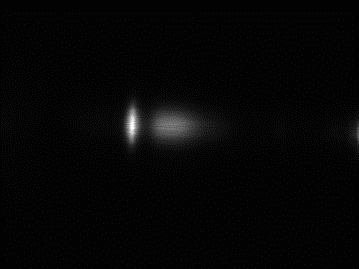
\includegraphics[width=8.8cm]{figures/p2-1.PNG} %插入图片,[]中设置图片大小,{}中是图片文件名
	\caption{全幅光譜影像} %最终文档中希望显示的图片标题
	\label{2.1,全幅光譜影像} %用于文内引用的标签
\end{figure}
圖像的像素對應於二維空間中一個特定的位置,而圖像的灰度值能表示出光的強度。圖\ref{2.1,全幅光譜影像}. 為三通道RGB彩色影像,透過灰階色彩轉換公式,則可將三通道轉為由灰度表示的單通道光度影像圖。轉換公式如式(\ref{eq:RBGtrans1})所示。
\begin{equation}
\label{eq:RBGtrans1}
Gray = R\times0.299 + G\times0.587 + B\times0.114
\end{equation}
為了提升程式運算速度,將三位精度浮點數算法縮放1000倍,修改為整數運算法
\begin{equation}
	\label{eq:RBGtrans2}
	Gray = (R\times299 + G\times587 + B\times114 + 500) / 1000
\end{equation}
整數運算雖提高運算速度,但在需要高精度的光譜分析時,使用位移運算法,即將公式(\ref{eq:RBGtrans2})中RGB的灰階轉換係數分別放大2的20次方倍,得到
\begin{equation}
	\label{eq:RBGtrans3}
	Gray = R\times313524.224 + G\times615514.112 + B\times119537.664
\end{equation}
將公式(\ref{eq:RBGtrans3})係數四捨五入成整數運算後得
\begin{equation}
	Gray = (R\times313524 + G\times615514 + B\times119538) >> 20
    \label{eq:2.4}
\end{equation}
其中$>>$為位元右移運算子,即將公式(\ref{eq:2.4})所求得結果轉換為二進制後向右位移二十位元,即可求得該像素灰階值。
\subsection{興趣區間(Region of Interest, ROI)}
一張全幅影像帶有所有光譜訊息,也伴隨著許多多餘的光譜訊息,若將全幅影像皆納入計算,則會造成運算量的大幅提升,且更容易受到環境光等因素的干擾,因此找出影像的興趣區間(ROI)為光譜分析的重要步驟之一。\par
假設一輸入全幅影像如圖\ref{2.1,全幅光譜影像}. 所示,將影像以縱向三等份後如圖\ref{2.2,全幅光譜影像縱向分區}. 所示,明顯可以看出圖\ref{2.2,全幅光譜影像縱向分區}. 中上下兩個無光區不帶有光譜訊息,而對於波長校正來說,ROI必需包含所有橫像素,並且以縱方向的光度平均值強弱為波長校正ROI的判定方式。
\begin{figure}[H] %H为当前位置,!htb为忽略美学标准,htbp为浮动图形
	\centering %图片居中
	\setlength{\abovecaptionskip}{0.6cm}
	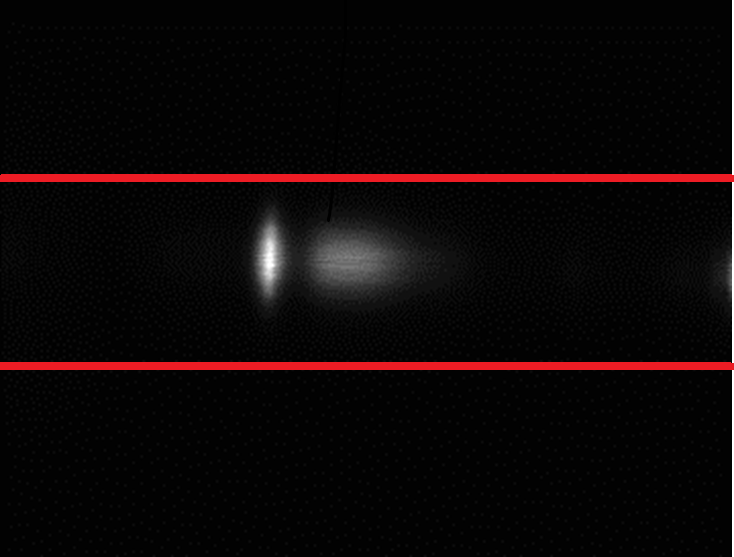
\includegraphics[width=8.8cm]{figures/p2-2.PNG} %插入图片,[]中设置图片大小,{}中是图片文件名
	\caption{全幅光譜影像縱向分區} %最终文档中希望显示的图片标题
	\label{2.2,全幅光譜影像縱向分區} %用于文内引用的标签
\end{figure}
\subsection{自動強度調整}
取出ROI光譜影像後,時常因影像感測器亮度參數過大、過小或光源強弱而導致影像無法分析。過曝影像之光譜會因其部份強度超過上限值,造成擬合參考點減少而計算出誤差極大的峰值位置,而過暗光譜影像之光譜會難以辨識雜訊與目標波峰,因此太弱或太高的強度都將導致後續分析處理的困難。
本文採用的影像感測器的可調參數分別為數位增益(Digital Gain, DG)、背光補償(Back Light, BL)與色差補償(Gamma)。各自的可調範圍顯示於表\ref{感測器參數}. 中。
\begin{center}
\vspace{0.8cm}
\captionof{table}{感測器參數範圍}\label{感測器參數}
\begin{tabularx}{\textwidth}{m{0.33\textwidth}<{\centering} m{0.33\textwidth}<{\centering} m{0.33\textwidth}<{\centering}}
	\hline\hline
	Name & Min & Max \\
	\hline
	DG & 32 & 255 \\
	\hline
	BL & 0 & 3\\
	\hline
	Gamma & 100 & 300 \\
	\hline\hline
\end{tabularx}
\vspace{10pt}
\end{center}
\par
由表\ref{感測器參數}. 可知,最適合細調的參數為DG\cite{DG},因其最小值與最大值差異最大且刻度最細,因此先固定其餘兩可變參數為最低值,再輸入不同的DG值獲得相對應的最大強度值I,將結果以數據組$(DG_i,I_i)$表示,又以知DG與光譜強度線性相關,故將兩組以上有效數據組直線擬合如圖\ref{DG與強度擬合結果圖}. 所示。
\begin{figure}[H] %H为当前位置,!htb为忽略美学标准,htbp为浮动图形
	\centering %图片居中
	\vspace{0.8cm}
	\setlength{\abovecaptionskip}{0.cm}
	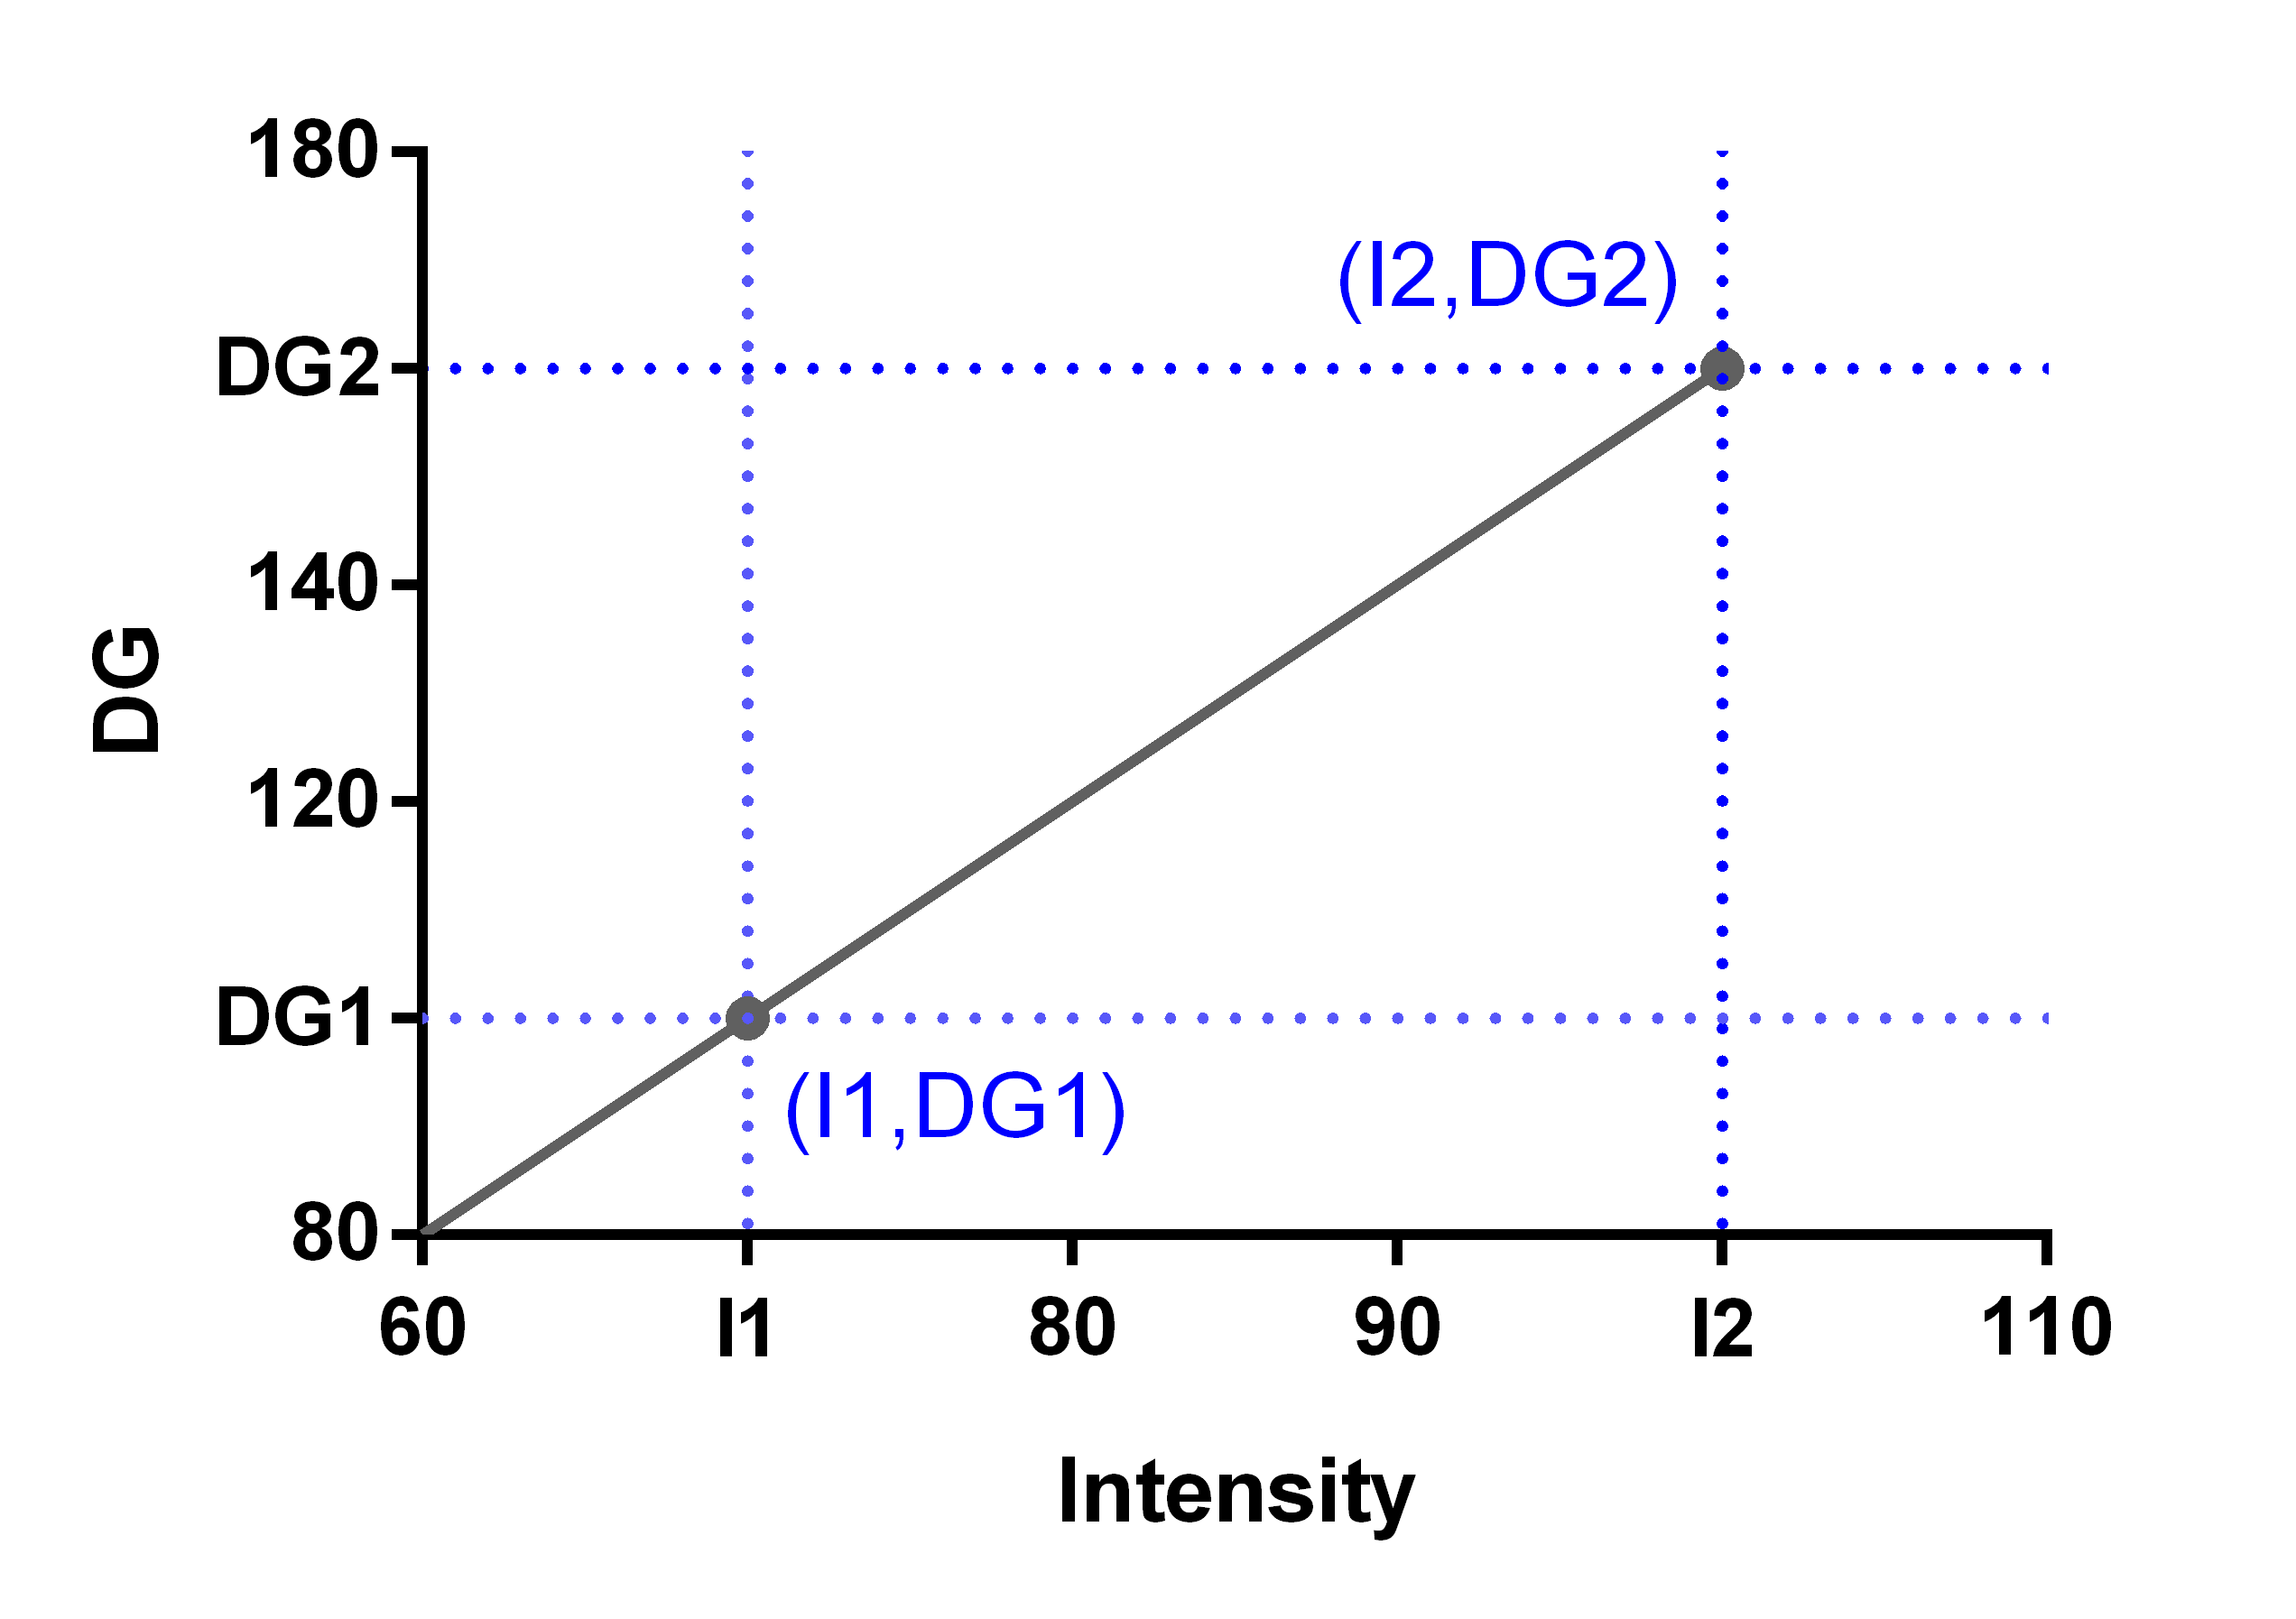
\includegraphics[width=13cm]{figures/AutoScaling.PNG} %插入图片,[]中设置图片大小,{}中是图片文件名
	\caption{DG與強度擬合結果圖} %最终文档中希望显示的图片标题
	\label{DG與強度擬合結果圖} %用于文内引用的标签
\end{figure}
今以數學式表示擬合直線為
\begin{equation}\label{eq:2.5}
	f(I) = aI+b\mid_{Gamma=100;BackLight=0}, \quad \forall a,b \in \mathbf{\mathbb{R}}
\end{equation}
由式(\ref{eq:2.5})可知,若欲將強度調整至$I_{max}$,則DG應設置為
\begin{equation}\label{eq:2.6}
	DG_{goal} = f(I_{max})\mid_{Gamma=100;BackLight=0}
\end{equation}
求出$DG_{goal}$並重新設置影像感測器參數後,即可獲得期望的最大強度值。
\section{Hilbert Transform運算}
在訊號理論中時常使用希爾伯特轉換(Hilbert Transform)\cite{Hilbert_book}估算粗略的信號峰值位置,本文中的峰值偵測演算法將利用Hilbert Transform找出粗略峰值像素位置並將信號分區。\par
一輸入訊號
\begin {math}
i(t) 
\end{math}
,與函數
\begin {math}
h(t) = \frac{1}{\pi t}
\end{math}
的卷積運算稱為Hilbert Transform,因此經Hilbert Transform後的輸出訊號表示為:
\begin{equation}\label{eq:2.7}
	y(t)=i(t)\ast h(t) = \frac{1}{\pi}\int_{-\infty}^{+\infty}i(t)\frac{1}{t-\tau}d\tau
\end{equation}
經由Hilbert Transform後的信號如圖\ref{單雷射波型經希爾伯特轉換}. 所示,輸入信號的峰值位置落在轉換後信號波谷與波峰的中心點,本文將此Hilbert Transform特性應用於3.5章波峰查找。
\begin{figure}[H] %H为当前位置,!htb为忽略美学标准,htbp为浮动图形
	\centering %图片居中
	\vspace{10pt}
	\setlength{\abovecaptionskip}{0.cm}
	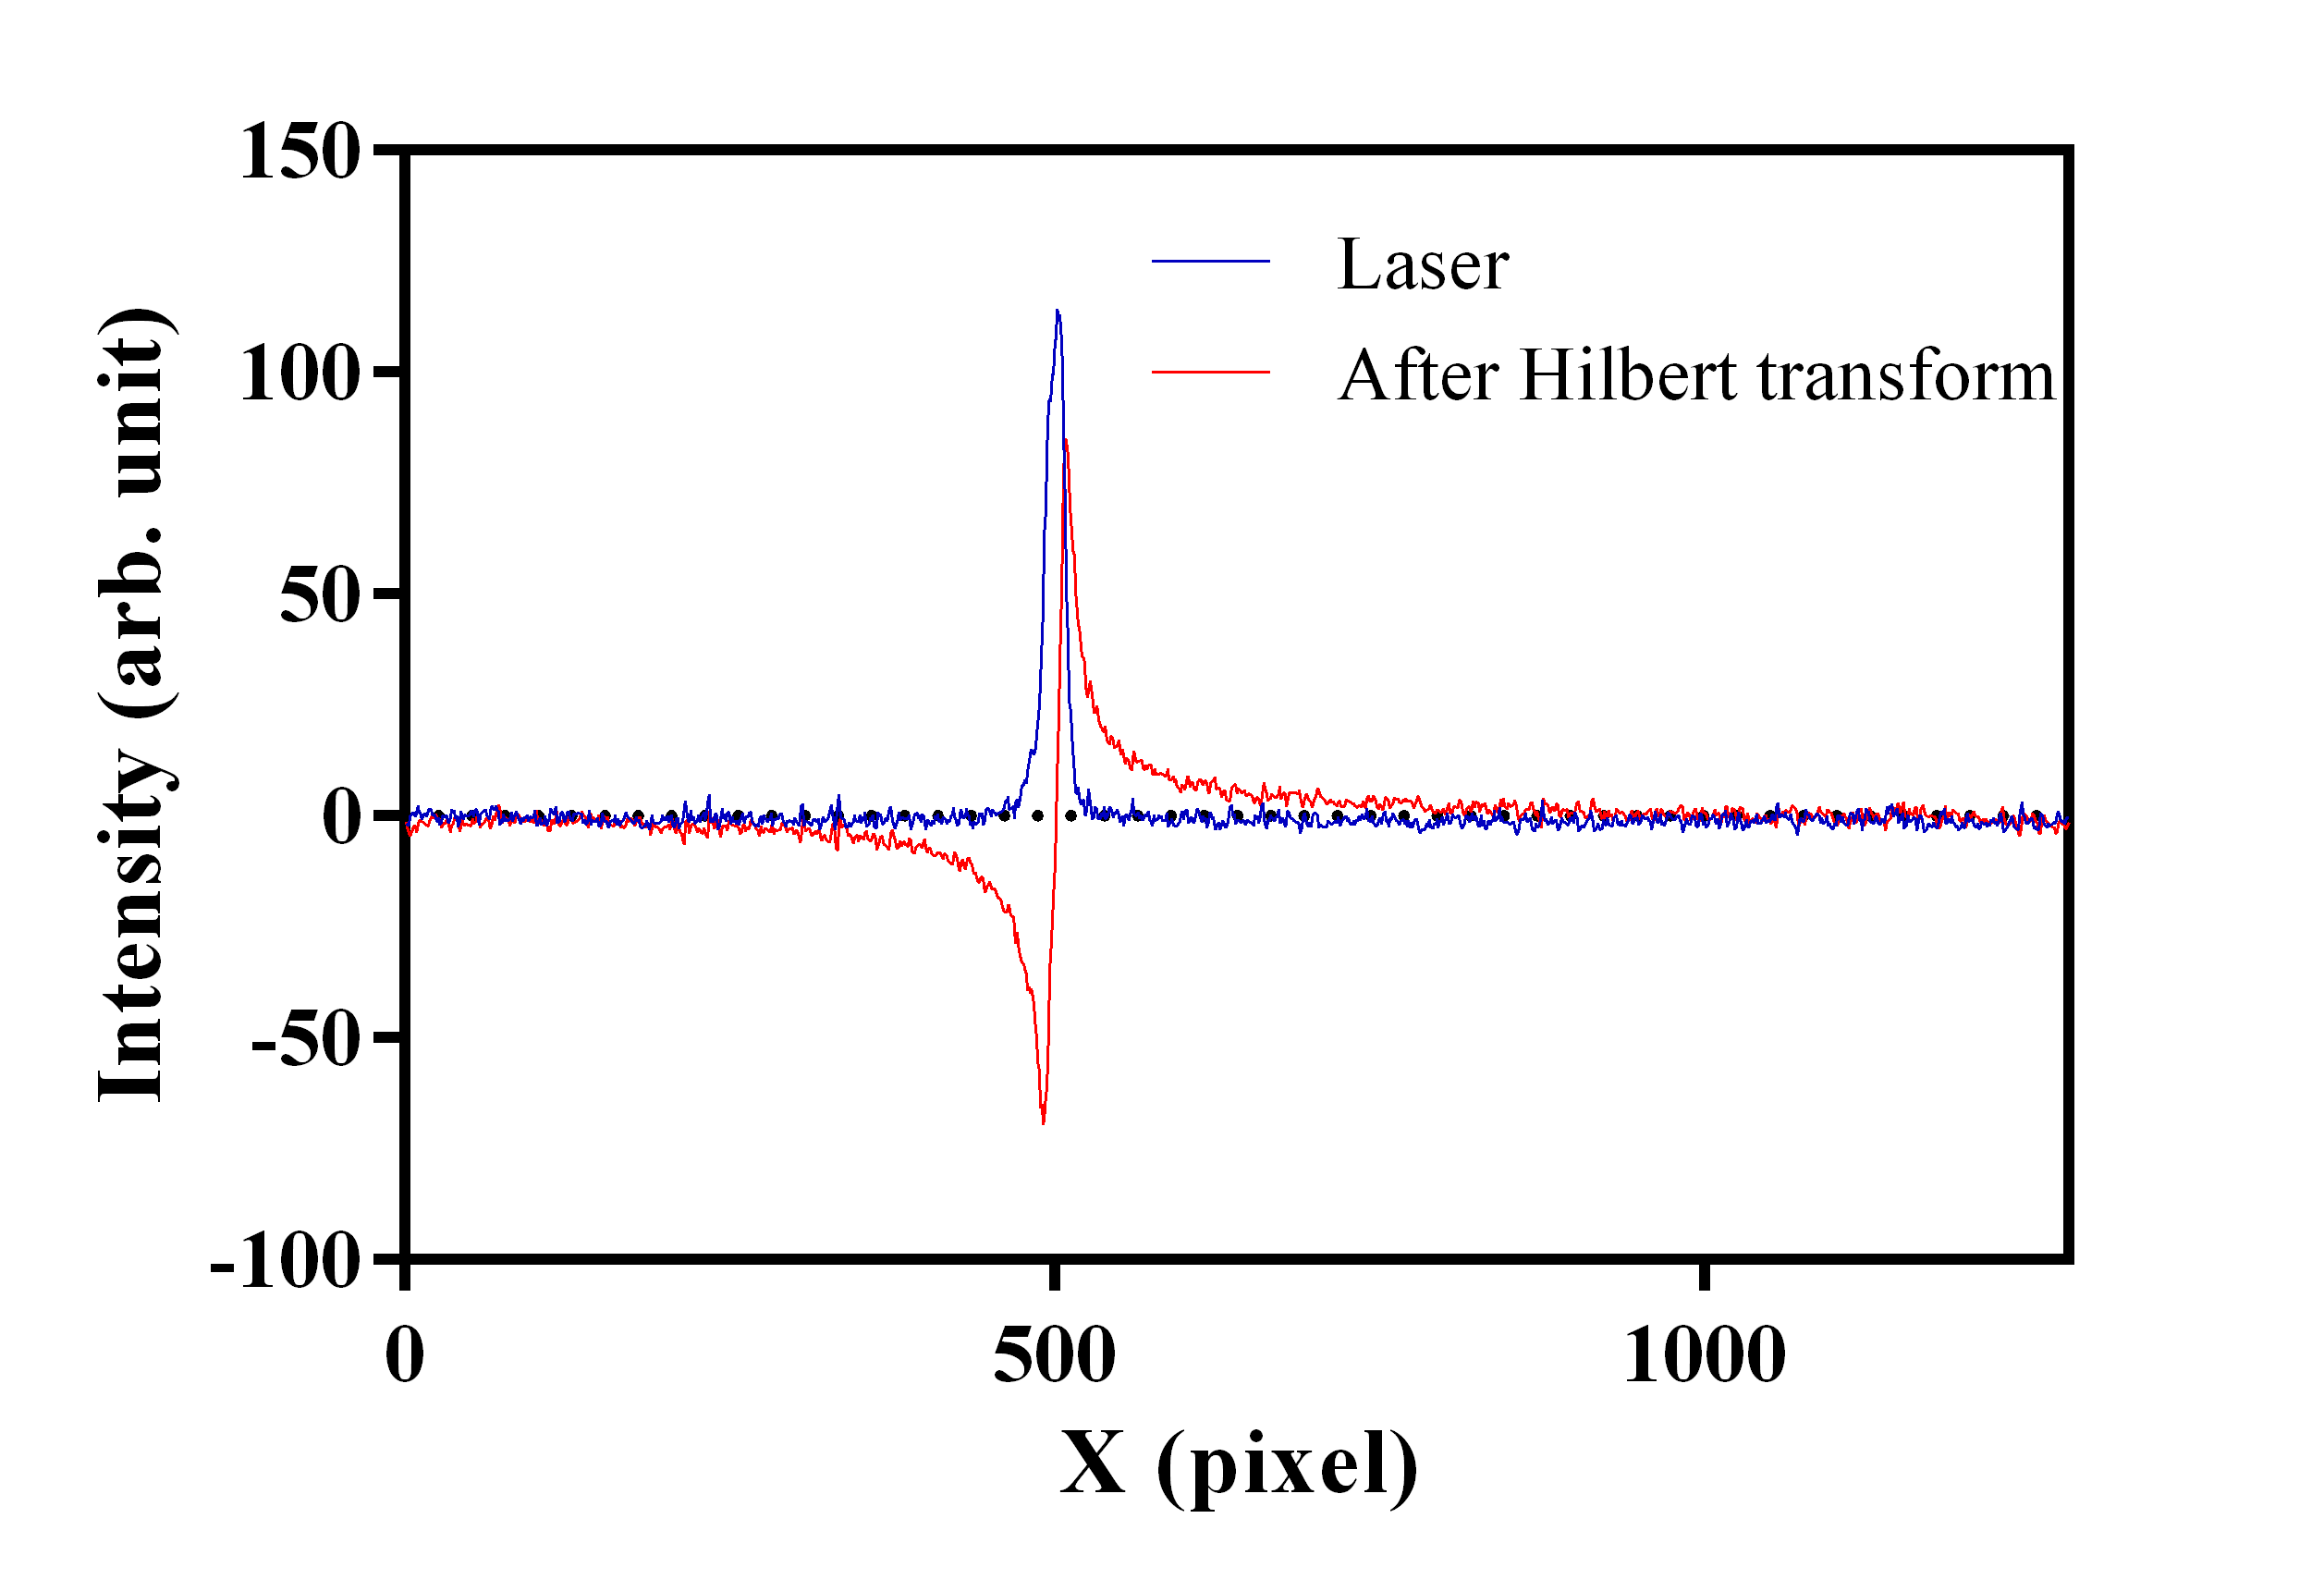
\includegraphics[width=16cm]{figures/p2-3_V2.png} %插入图片,[]中设置图片大小,{}中是图片文件名
	\caption{單雷射波型經Hilbert Transform轉換} %最终文档中希望显示的图片标题
	\label{單雷射波型經希爾伯特轉換} %用于文内引用的标签
\end{figure}
\section{光譜模型擬合}
光譜波形分析使用曲線擬合\cite{Spectral-fitting}的原因通常為分離不同波段光譜,但對於波長校正來說,使用曲線擬合的主要原因為以下兩點:
\par
	\textbf{一.} 光譜因環境光等眾多因素,導致波形失真,使用波形擬合可以將光譜逼近於完美波形,使光譜分析更加容易,圖\ref{雷射波形高斯擬合前後}. 為高斯擬合前後的結果對比。
	\begin{figure}[H]
		\centering
		\vspace{0.8cm}
		%\setlength{\belowcaptionskip}{-1cm} 
		\begin{subfigure}[fig nice]{0.49\textwidth}
			\setlength{\abovecaptionskip}{0.cm}
			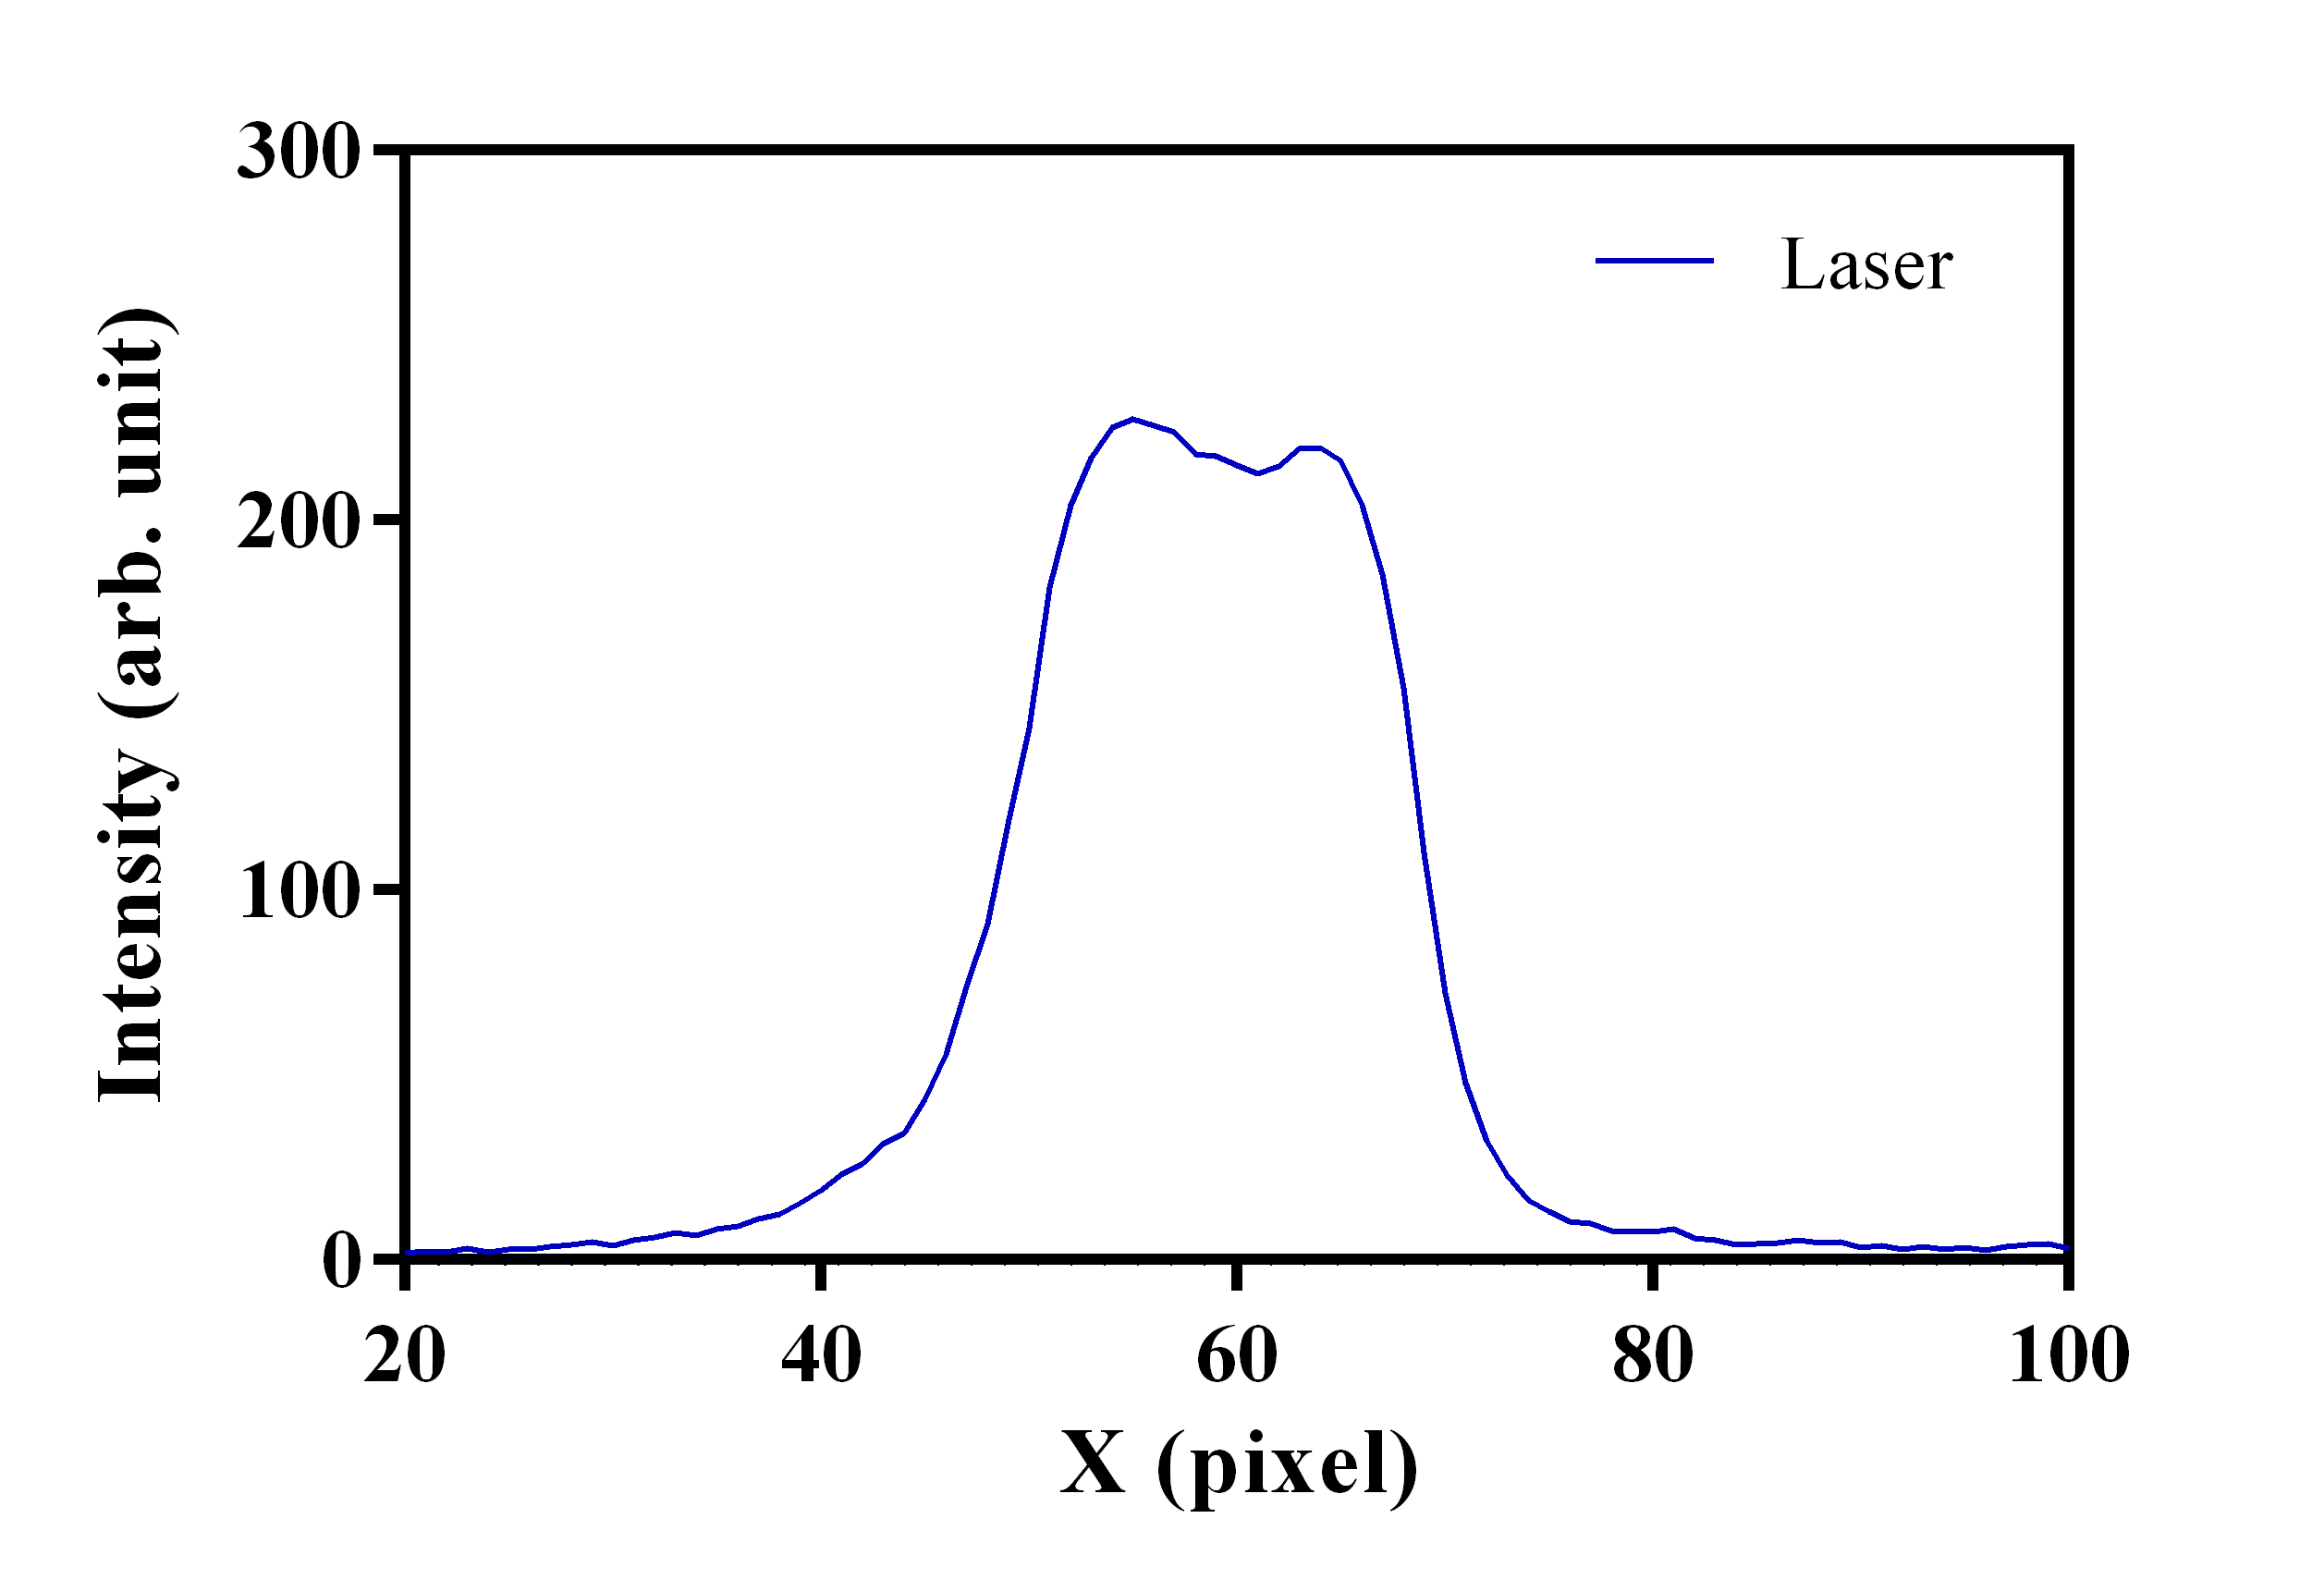
\includegraphics[width=7.9cm]{figures/Laser1.png}
			\caption{}
			%\subcaption{雷射波形}
			\label{雷射波形}
		\end{subfigure}
		\begin{subfigure}[fig nice]{0.49\textwidth}
			\setlength{\abovecaptionskip}{0.cm}
			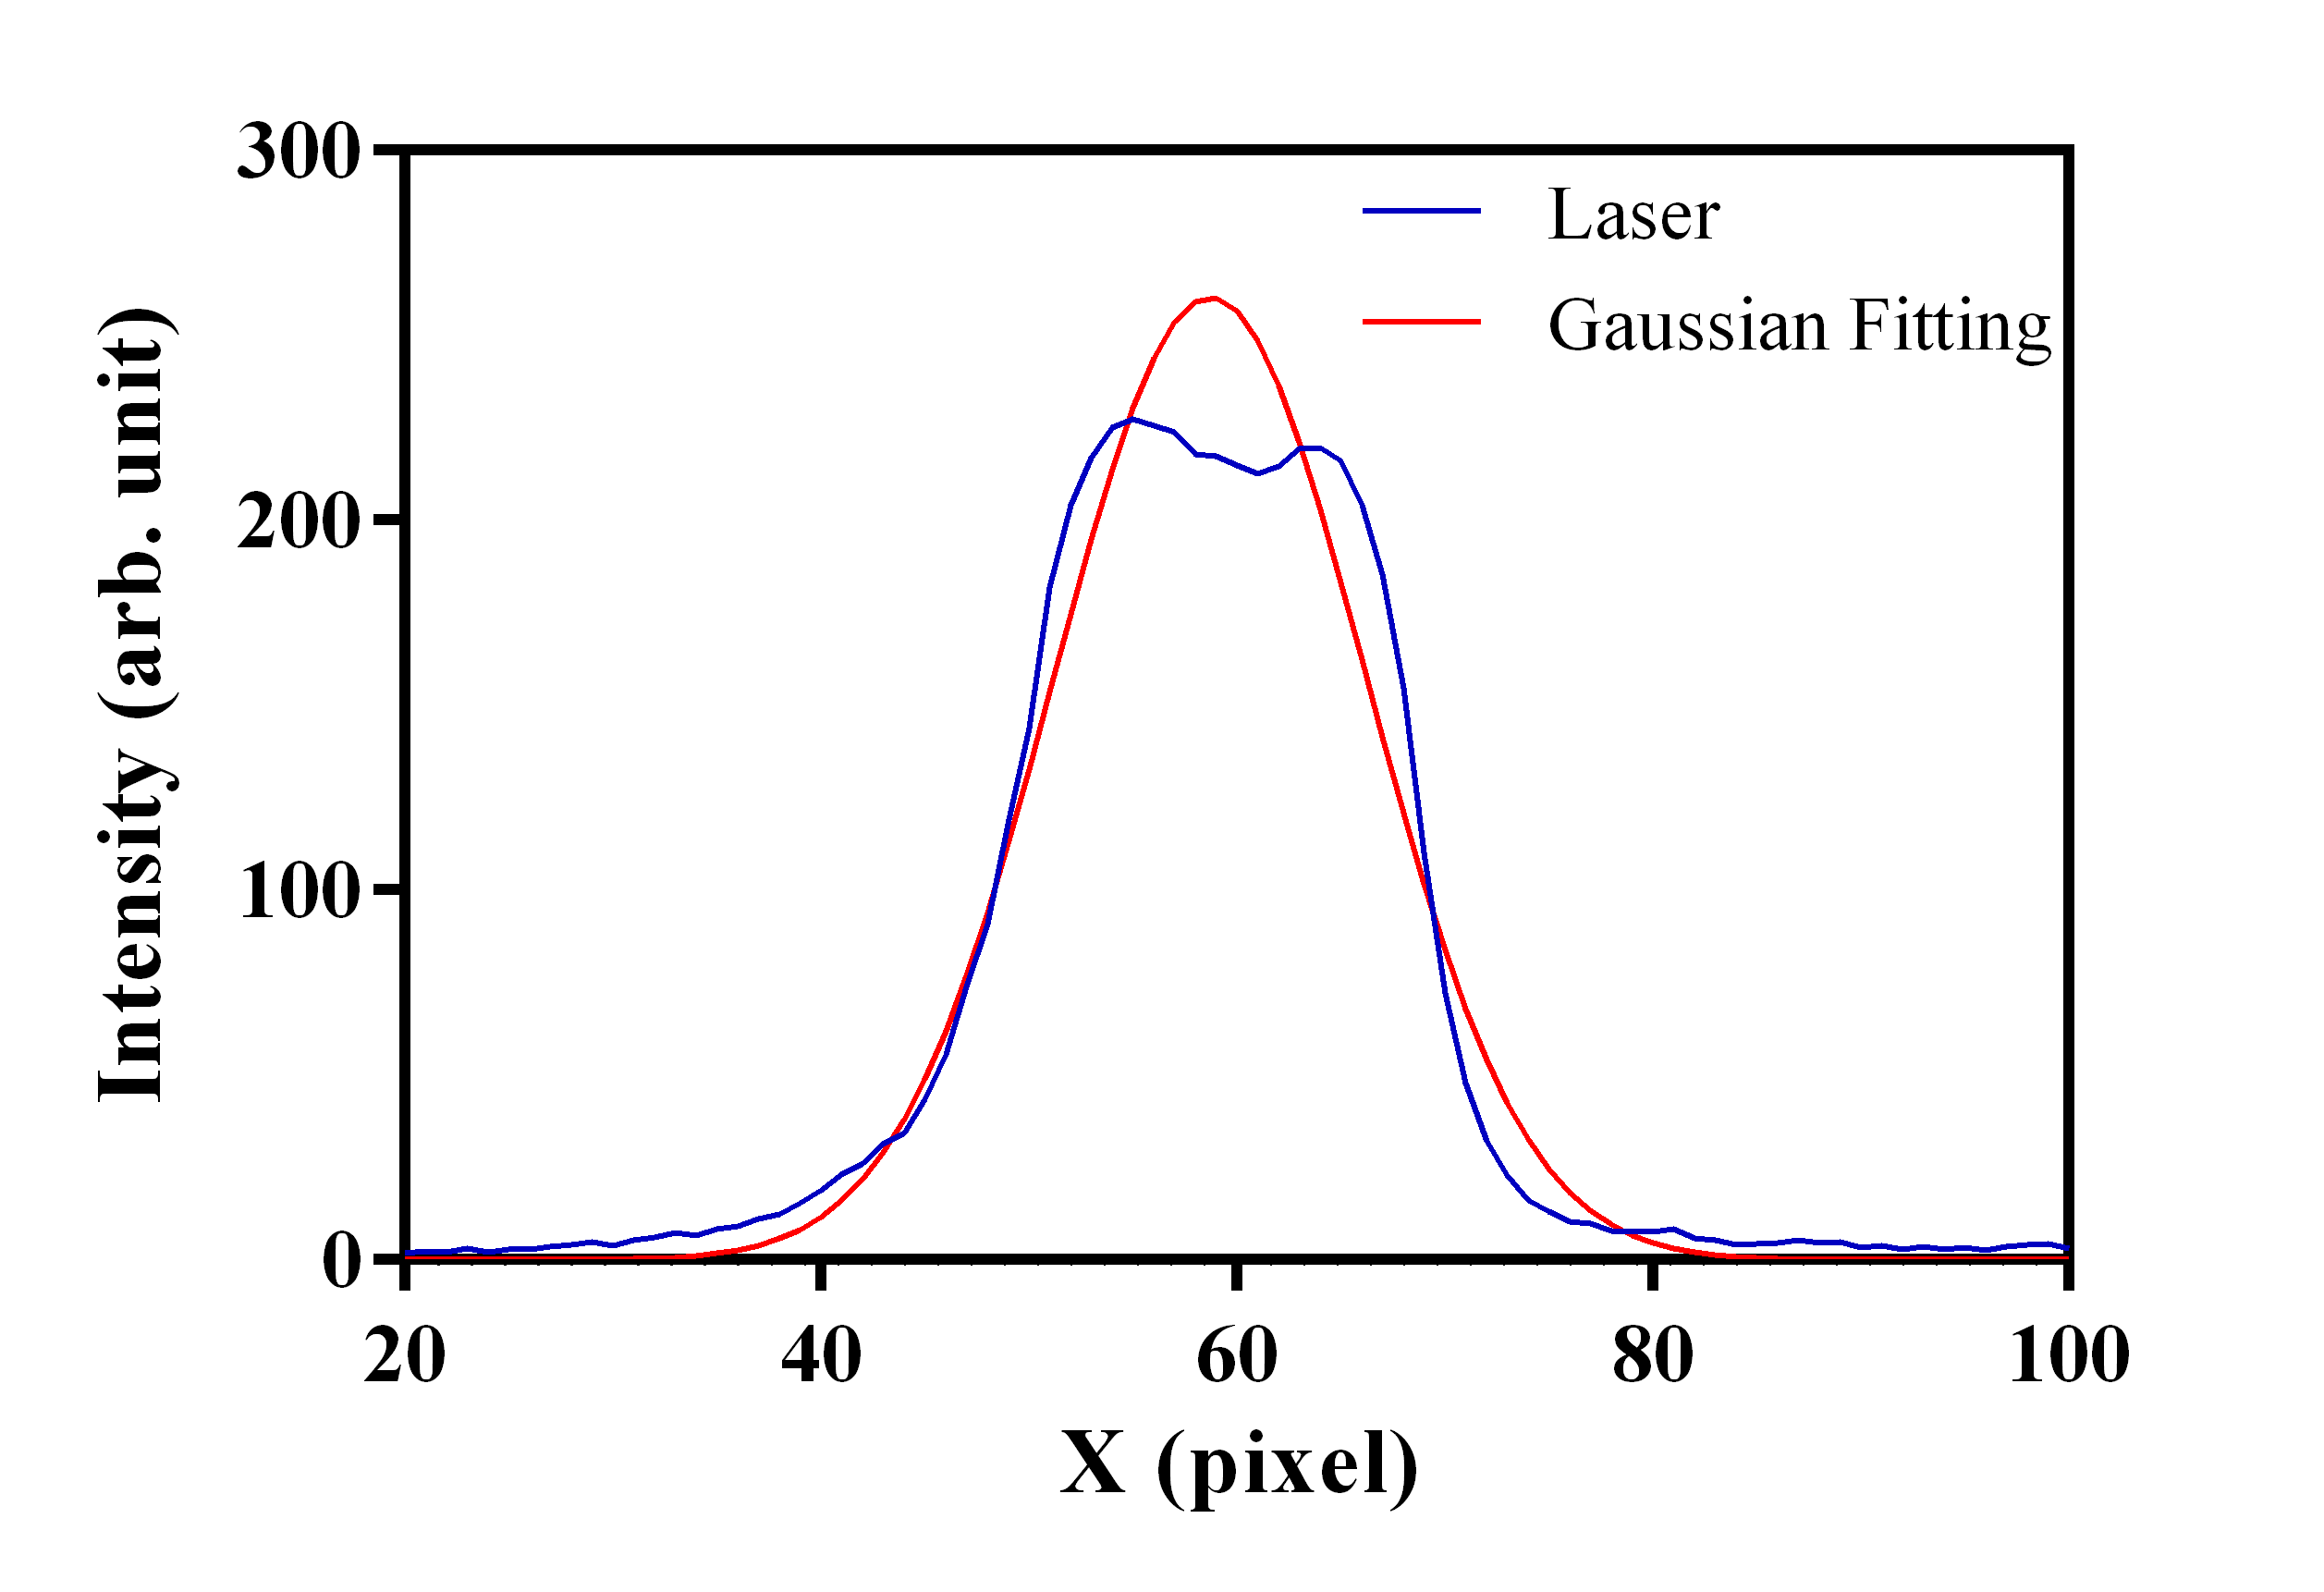
\includegraphics[width=7.9cm]{figures/Gassian_NEW600.png}
			\caption{}
			%\subcaption{高斯擬合後之雷射波形}
			\label{雷射經高斯擬合後}
		\end{subfigure}
	%\caption{雷射波形高斯擬合前後}
	\caption[失真嚴重的雷射波形高斯擬合前後比較圖]{雷射波形高斯擬合前後比較 (a)雷射原始波形(b)高斯擬合後之雷射波形}
	\label{雷射波形高斯擬合前後}
	\end{figure}
\textbf{二.} 當一光源進入影像感測器後,光源中心點受限於影像感測器像素值,無法精確表達出波峰正確位置。假設一完美無干擾光源波峰位置落在像素x = 404.35 pixel處,若單純由最高值方式偵測波峰,僅能找出x = 404 pixel,若採用波形擬合,可以利用其餘數據點加入模型擬合來找出最準確的波峰位置,表\ref{峰值位置比較表}. 顯示六束不同波長雷射的最大值位置與高斯擬合找出的最大值位置比較。
\begin{center}
\vspace{0.8cm}
\captionof{table}{峰值位置比較表}\label{峰值位置比較表}
\begin{tabularx}{\textwidth}{|c|m{1.5cm}<{\centering}|m{1.5cm}<{\centering}|m{1.5cm}<{\centering}|m{1.5cm}<{\centering}|m{1.41cm}<{\centering}|}
	\hline
	原始最大值位置(pixel)& 358 & 407 & 505 & 650 & 813\\
	\hline
	高斯擬合後最大值位置(pixel)& 357.69 & 406.85 & 504.52 & 650.26 & 812.72\\
	\hline
	誤差(pixel)&-0.31&-0.15&-0.48&0.26&-0.28\\
	\hline
\end{tabularx}
\vspace{10pt}
\end{center}

\subsection{高斯擬合}
高斯模型的函數\cite{Lorentz_AND_GAUSSIAN_book}形式為:
\begin{equation}\label{eq2.8}
	f(x)=a e^{\frac{-(x-b)^2}{2c^2}} \quad , \quad \forall a,b,c \in \mathbf{\mathbb{R}}
\end{equation}
今假設有一光譜數據組$(P_i,y_i)$其中$i=1,2,3,\cdots$欲使用高斯函數擬合,將此數據組以高斯函數描述:
\begin{equation}\label{eq2.9}
	y_i=y_{max} e^{\frac{-(P_i-P_{max})^2}{S}}
\end{equation}
其中的待估實數常數$y_{max}$、$P_{max}$與$S$分別代表高斯曲線的峰值、峰值位置與半高全寬訊息。將(\ref{eq2.9})
等號兩端取對數,化成:
\begin{equation}\label{eq2.10}
	\ln{y_i}=\ln{y_{max}}-\frac{(P_i-P_{max})^2}{S} = (\ln{y_{max}}-\frac{P_{max}^{2}}{S})+\frac{2P_i P_{max}}{S}-\frac{P_{i}^{2}}{S}
\end{equation}
令: 
\begin{equation}\label{eq2.11}
	\begin{cases}
		& \ln{y_i} = z_i \\
		& \ln{y_{max}}-\frac{P_{max}^{2}}{S} = b_0\\
		& \frac{2 P_{max}}{S} = b_1\\
		&  -\frac{1}{S} = b_2
		\end{cases}
\end{equation}\\
將(\ref{eq2.11})帶回(\ref{eq2.10})中替換,並以矩陣型式表示:
\\
\begin{equation}\label{eq2.12}
\begin{bmatrix} z_1\\z_2\\z_3\\ \vdots\\z_n\end{bmatrix} 
 \quad
= 
 \quad
 \begin{bmatrix} 
 	1&P_1&P_{1}^{2}\\
 	1&P_2&P_{2}^{2}\\
 	1&P_3&P_{3}^{2}\\
 	\vdots&\vdots&\vdots\\
 	1&P_n&P_{n}^{2}
 \end{bmatrix}
\begin{bmatrix} b_0\\b_1\\b_2 \end{bmatrix} 
\end{equation}
簡記(\ref{eq2.12})式為:
\begin{equation}\label{eq2.13}
  Z = PB
\end{equation}
則特徵參數矩陣$B$的最小二乘方解\cite{Least-Squart-method}為:
\begin{equation}\label{eq2.14}
	B = (P^TP)^{-1}P^T Z
\end{equation}
再根據式(\ref{eq2.11})求出$y_{max}$、$P_{max}$與$S$,即可求得高斯函數的峰值、峰值位置與半高全寬。

\subsection{勞倫茲擬合}
勞倫茲函數\cite{Lorentz_AND_GAUSSIAN_book}的函數形式為:
\begin{equation}\label{eq2.15}
	f(x)=\frac{I}{1+(\frac{x-p}{\gamma})^2}
\end{equation}
其中$I$為最大值,$p$為最大值位置,$\gamma$為半高全寬參數,其半高全寬為$2\gamma$,今假設有一組數據$(x_i,yi)$其中$i=1,2,3,\cdots$,欲以勞倫茲函數進行數據擬合,將數據組以勞倫茲函數表示:
\begin{equation}
	f_i= \frac{I_{max}}{1+(\frac{x_i-p_{0}}{\gamma})^2}
	\label{eq2.16}
\end{equation}
展開式(\ref{eq2.16})可得:
\begin{equation}\label{eq2.17}
	\frac{1}{f_i}= \frac{1}{I_{max}}(1+\frac{p_0^2}{\gamma^2})-\frac{2p_0}{I_{max}\gamma^2}x_i+\frac{1}{I_{max}\gamma^2}x_{i}^{2}
\end{equation}
令: 
\begin{equation}\label{eq2.18}
	\begin{cases}
		& \frac{1}{f_i} = z_i \\
		& \frac{1}{I_{max}}(1+\frac{p_0^2}{\gamma^2}) = b_0\\
		& -\frac{2p_0}{I_{max}\gamma^2} = b_1\\
		&  \frac{1}{I_{max}\gamma^2} = b_2
	\end{cases}
\end{equation}\\
將式(\ref{eq2.18})帶回(\ref{eq2.17})替換,並以矩陣表示為:
\\
\begin{equation}\label{eq2.19}
	\begin{bmatrix} z_1\\z_2\\z_3\\ \vdots\\z_n\end{bmatrix} 
	\quad
	= 
	\quad
	\begin{bmatrix} 
		1&x_1&x_{1}^{2}\\
		1&x_2&x_{2}^{2}\\
		1&x_3&x_{3}^{2}\\
		\vdots&\vdots&\vdots\\
		1&x_n&x_{n}^{2}
	\end{bmatrix}
	\begin{bmatrix} b_0\\b_1\\b_2 \end{bmatrix} 
\end{equation}
\\
簡記(\ref{eq2.19})式為:
\begin{equation}\label{eq2.20}
	Z = XB
\end{equation}
則特徵參數矩陣$B$的最小二乘方解為:
\begin{equation}\label{eq2.21}
	B = (X^TX)^{-1}X^T Z
\end{equation}
再將參數矩陣$B$之參數$b_0$、$b_1$與$b_2$帶回式(\ref{eq2.18})解聯立方程式得出$I_{max}$、$p_{0}$與$\gamma$。














% !TeX root = ../main.tex
\titlespacing{\chapter}{0cm}{-2cm}{0cm}
\chapter{自動波長校正流程}

由第二章可知,自動波長校正需要大量矩陣運算,因此採用Matlab攥寫演算法,並打包成動態函式庫匯入基於.NET Framework架構下的Windows Form中使用,其運作方式如圖\ref{DLL檔運作圖}. 所示,又由於程式需要同步顯示即時光譜變化並同時進行取像、分析即感測器參數調整,故程式以多續程架構處理,以達目標功能,所有實現流程如圖\ref{程式架構總體流程圖}. 所示。\par
演算法首先透過RS-232與雷射光源機台溝通,發送點亮指定波長雷射後,當第一幀影像被取出後,首先將分析所需的ROI範圍,獲得ROI範圍後為了光譜分析的容易性,而調整影像參數,即Auto Scaling光譜最大值至使用者指定強度,接著透過希爾伯特轉換與高斯擬合或勞倫茲擬合找出精確的波峰位置,將結果數值存於記憶體(Memory)後,演算法將會再點亮下一根雷射光源重複此流程直至所有雷射與汞氬燈皆測量完畢。\par
在獲得所有包含汞氬燈的波峰與所有雷射的波峰後,將所有波峰像素位置與所有雷射標準波長進行三次多項式擬合,得出空間轉換多項式,並將所有像素帶入計算出實際轉換後波長位置與標準波長之RMS。

\begin{figure}[H] %H为当前位置,!htb为忽略美学标准,htbp为浮动图形
	\vspace{0.8cm}
	\centering %图片居中
	\setlength{\abovecaptionskip}{1cm}
	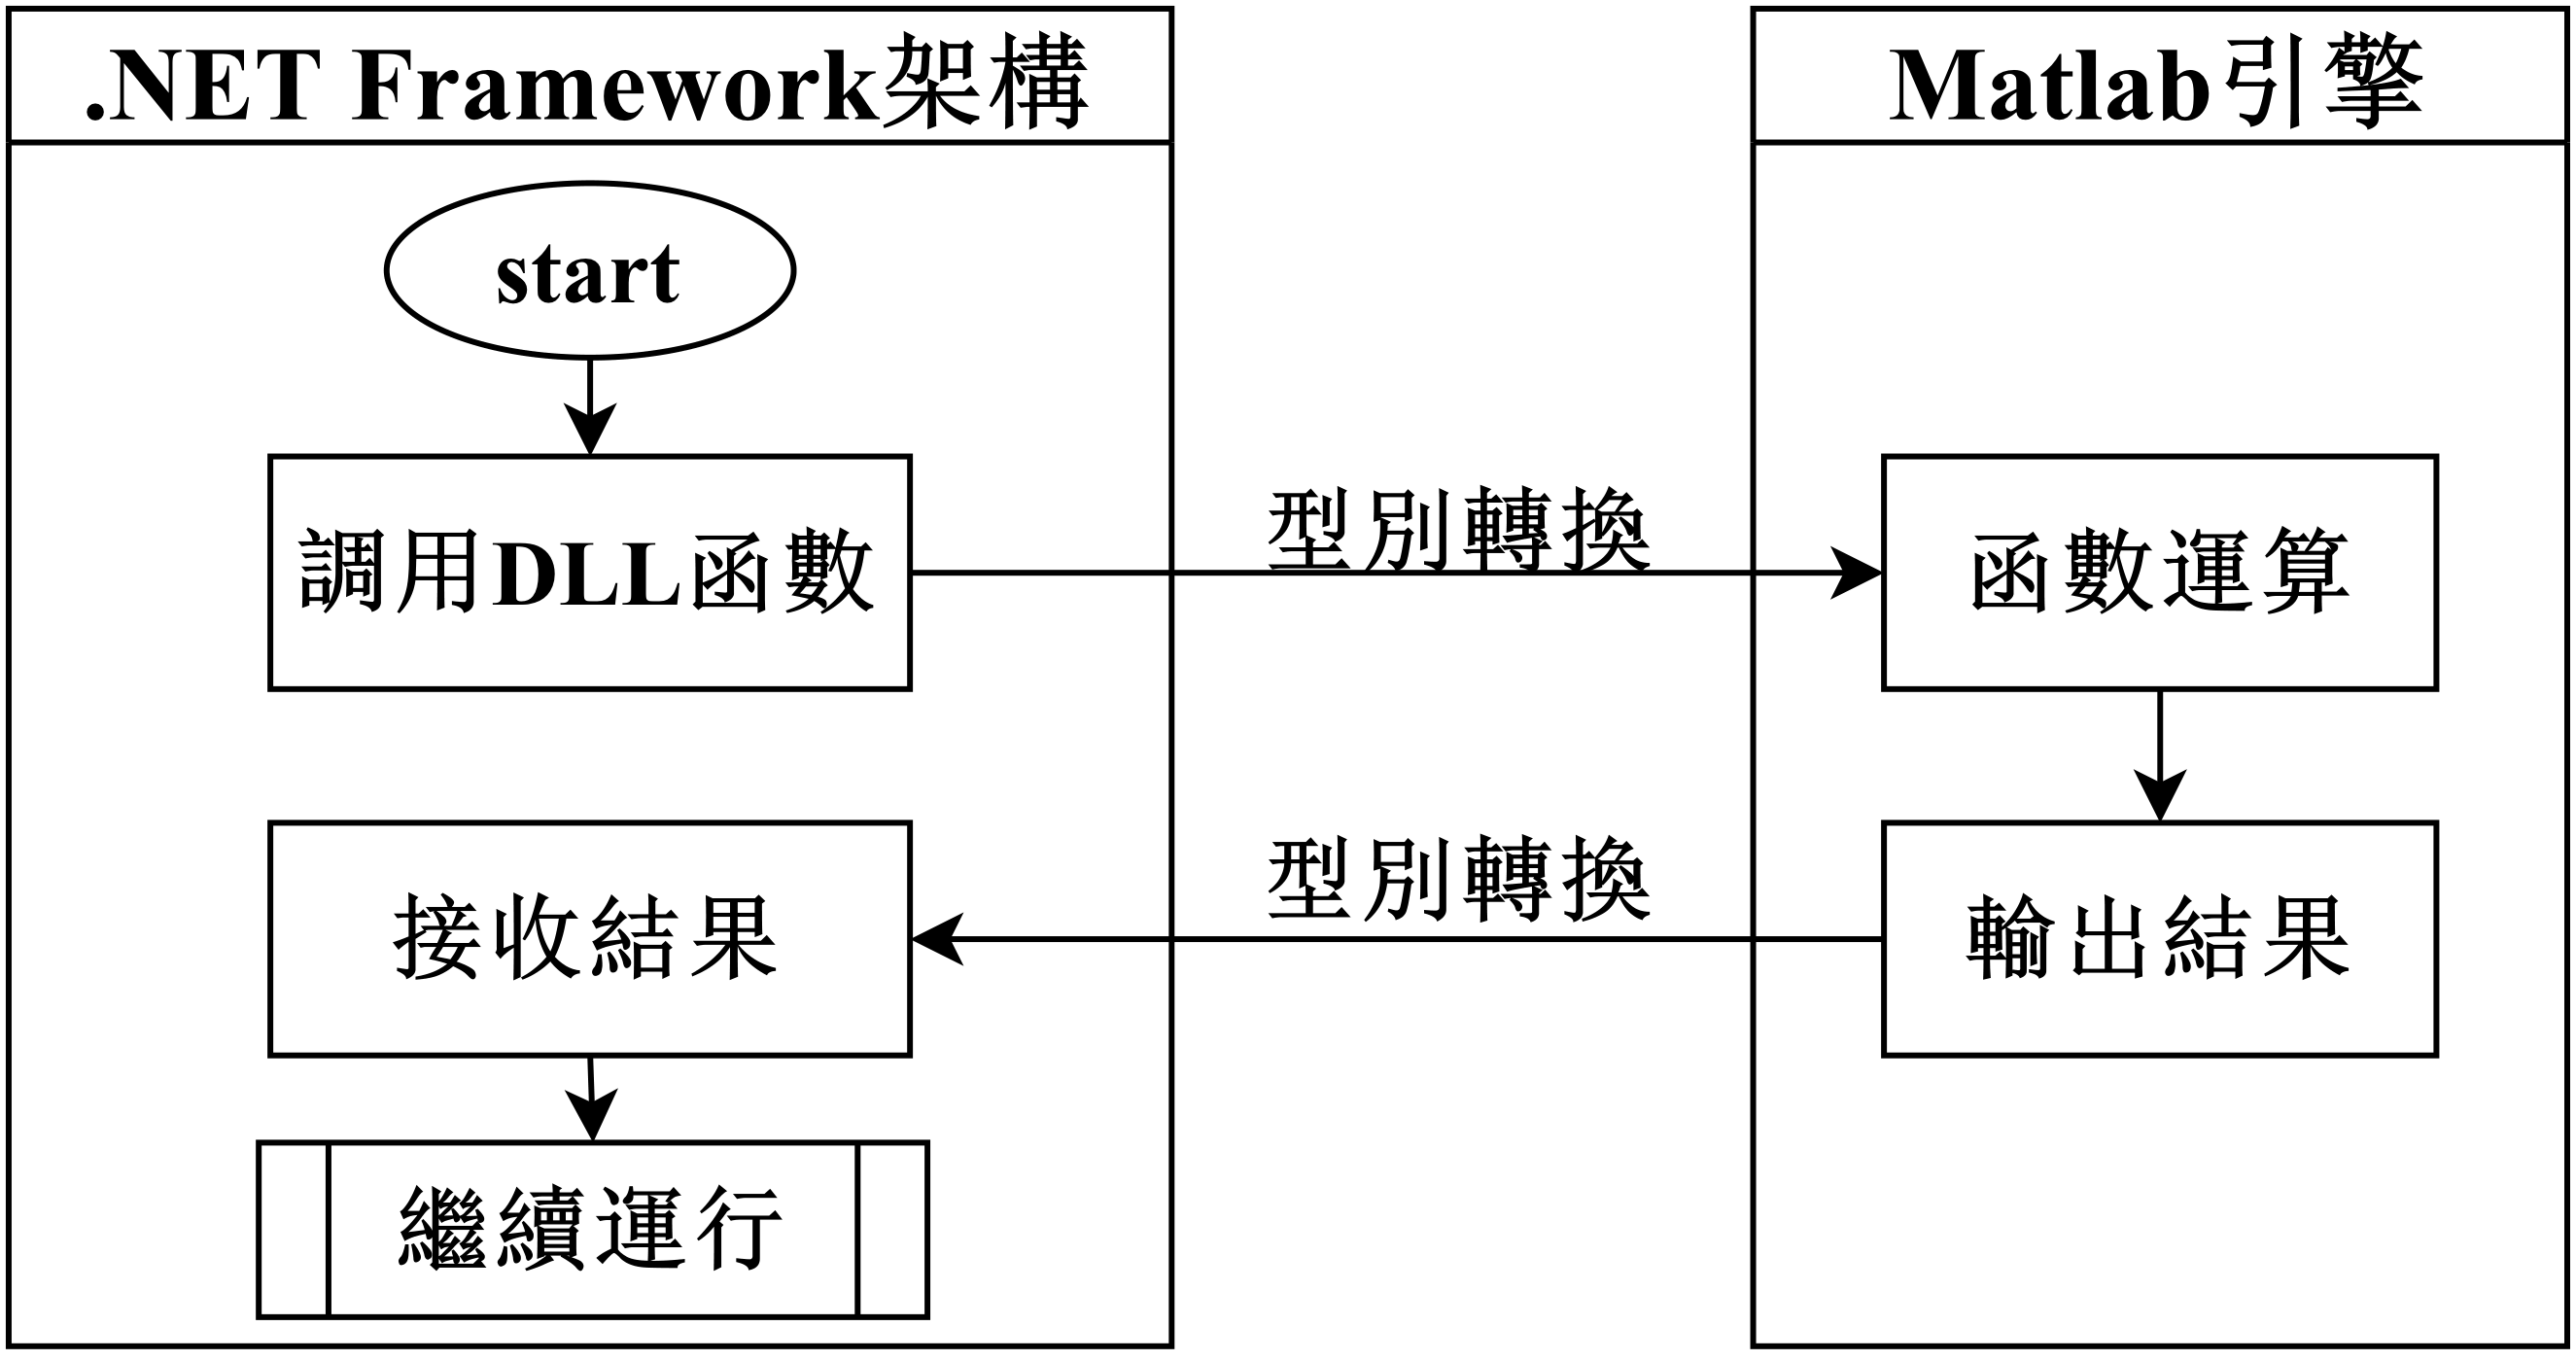
\includegraphics[width=0.8\textwidth]{figures/DLL.png} %插入图片,[]中设置图片大小,{}中是图片文件名
	\caption{DLL檔運作圖} %最终文档中希望显示的图片标题
	\label{DLL檔運作圖} %用于文内引用的标签
\end{figure}
\newpage
\begin{figure}[H] %H为当前位置,!htb为忽略美学标准,htbp为浮动图形
	\centering %图片居中
    \setlength{\abovecaptionskip}{1cm}
	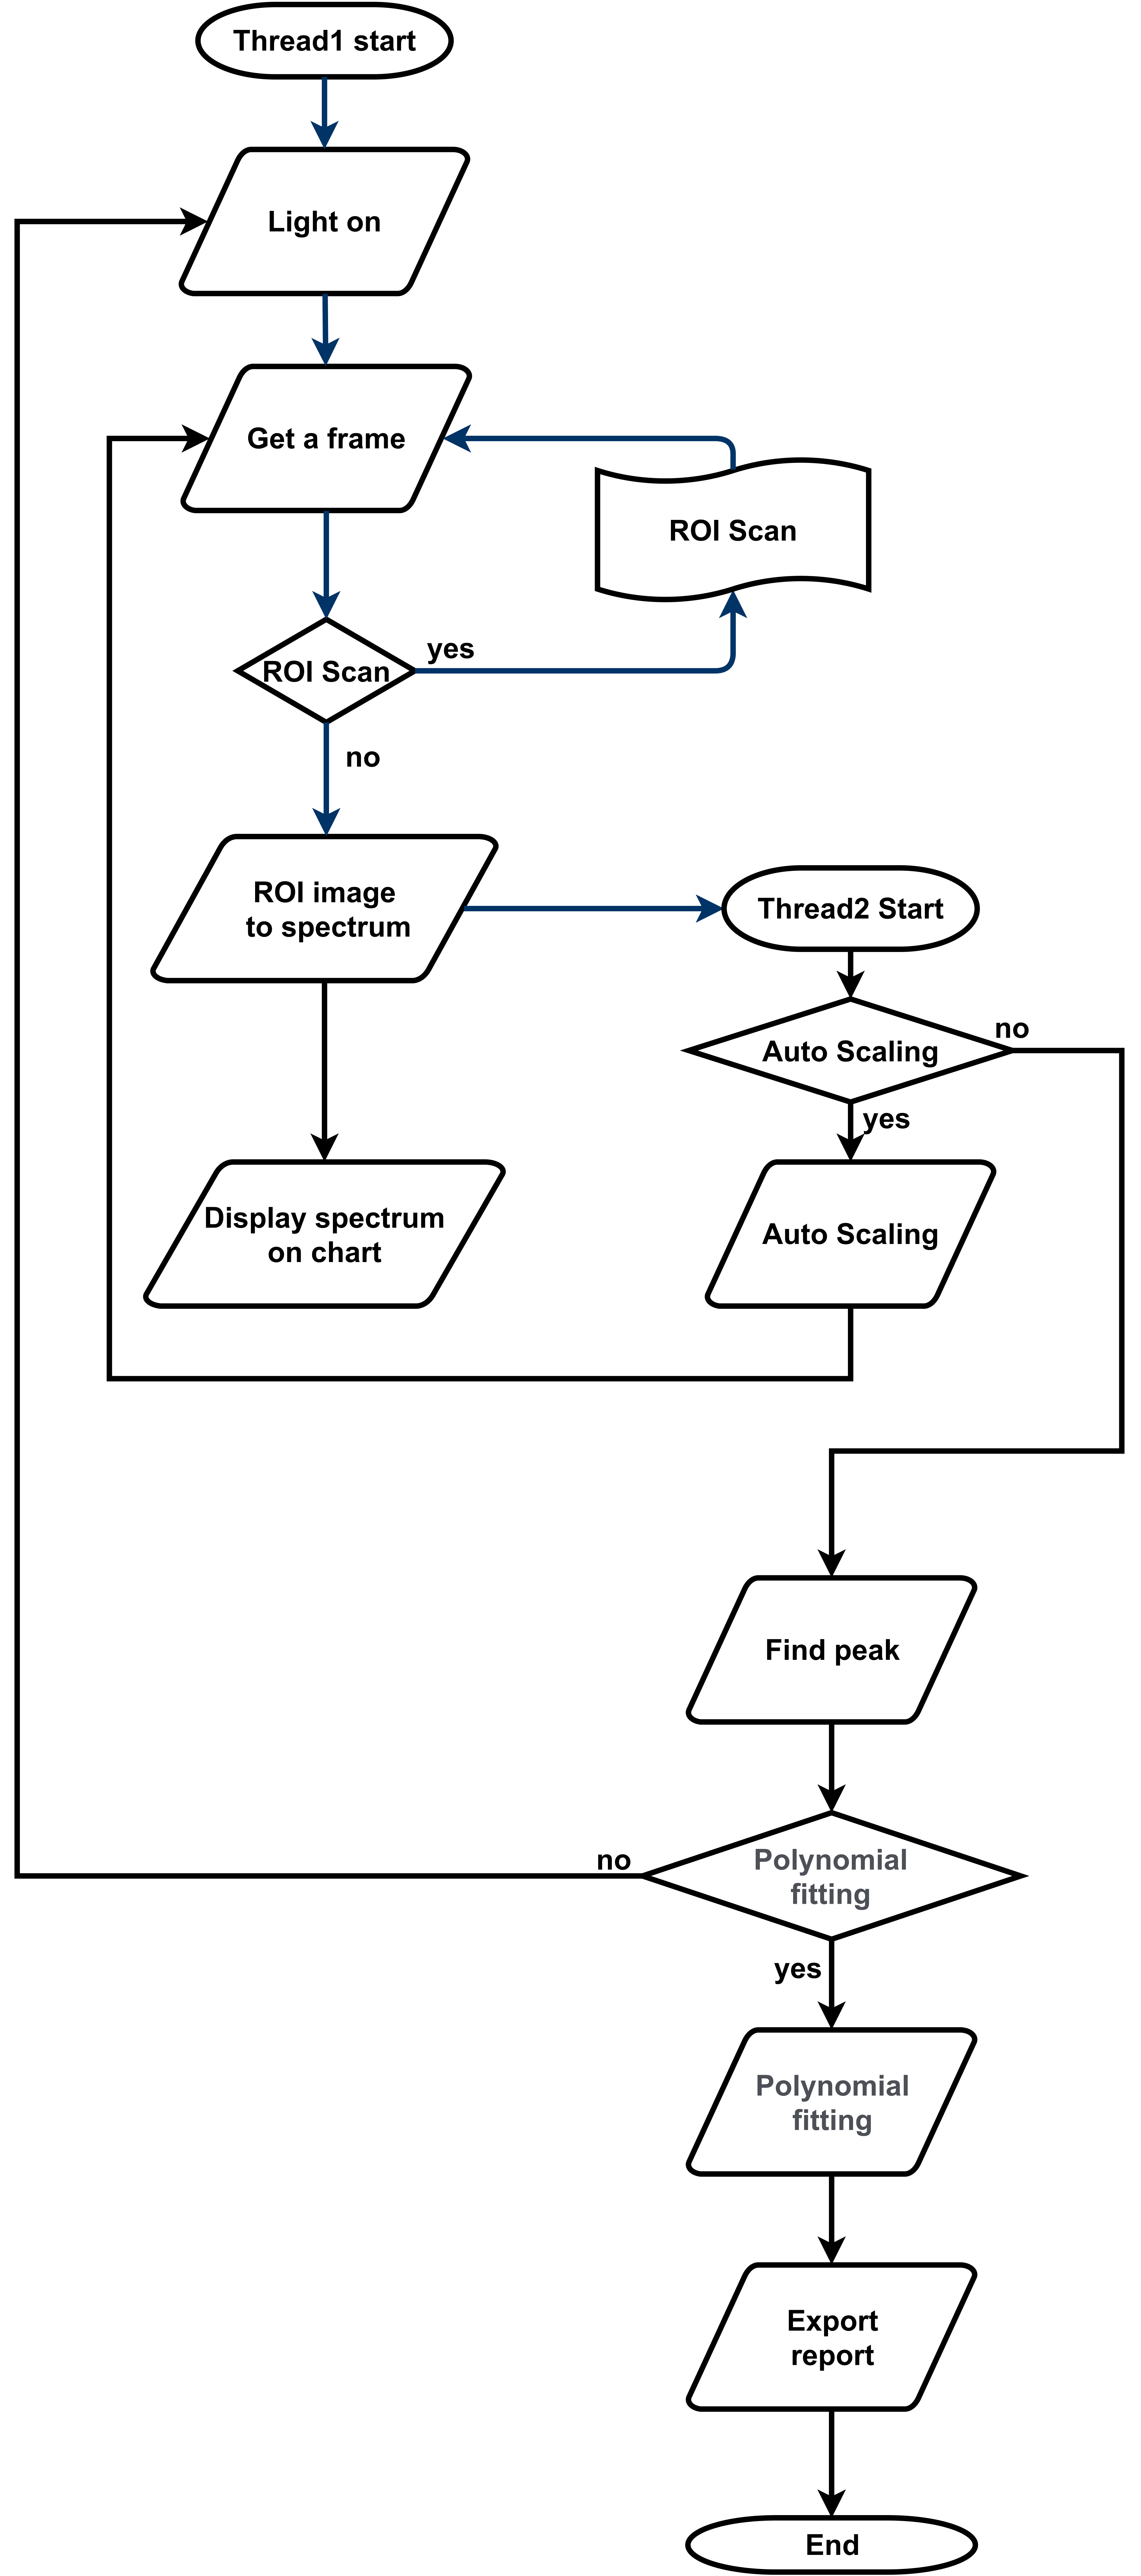
\includegraphics[width=0.6\textwidth]{figures/總流程圖.png} %插入图片,[]中设置图片大小,{}中是图片文件名
	\caption{軟體架構總流程圖} %最终文档中希望显示的图片标题
	\label{程式架構總體流程圖} %用于文内引用的标签
\end{figure}
\newpage
\section{動態連結函式庫}
動態連結函式庫(Dynamic-link library,縮寫為DLL),是為滿足使用者需要共享函式庫而由微軟在微軟視窗作業系統(Windows Form)中推出的實現方式,動態連結的意思是把時常所需要共享的的程式碼打包成DLL檔\cite{DLL},則當程式執行呼叫到DLL檔內的程式碼時,DLL可執行檔才會被系統載入到記憶體中運行,如圖\ref{DLL檔運作圖}. 所示,也因此動態連結方式僅在有需要時呼叫,可以大幅減低效能與記憶體浪費。\par
動態連結函式庫除了以上幾個主要優點外,DLL檔還能以Matlab編輯功能函數並導入其他語言架構中使用,因此在C\#語言架構下難以實現的複雜數學運算,便可以先透過Matlab建構功能函數,以達到簡化與加速複雜的演算法是本文採用動態連結函式庫的主要原因。\par
另外採用DLL檔的重要原因還有其通用性,因本研究之演算法全部皆採取Matlab編寫,而透過在Matlab中將演算法編寫成Function形式,則在打包成DLL檔後,不管在任何程式語言的架構下,只要輸入需要的輸入參數,皆可以在將資料進行型別轉換後透過DLL檔傳送給Matlab引擎進行計算,如此一來此演算法則具有良好的通用性,不管是使用C++或C語言等軟體開發時,都可以透過DLL檔使用本研究演算法。\par
由第二章使用的演算法運算過程可以看出本研究所使用的演算法需要大量的矩陣運算,因此透過DLL的方式,可由開發的C\#使用者介面,讓使用者能有簡易與美觀的操作介面,並在此建立主要的軟體架構,在此環境下所獲取的影像與資料數據,再透過型別轉換傳送至Matlab運算,經由Matlab引擎的運算可以大幅降低運算過程、所需時間與編譯複雜度,完成運算後的結果再經過資料型別轉換後傳送回原本的軟體架構中,如此一來便可以同時維持軟體的美觀與使用者操作體驗,並且可以進行相當複雜的運算,而且不需提高運算時間與編寫的複雜度。
\section{ROI Scan}
在進行影像與光譜之間的轉換之前,ROI Scan是必經的重要步驟之一。當一影像經由影像感測器取出,若將影像以矩陣方式表示如式(\ref{eq3.1}),則座標原點落於影像的最左上點即(x = 0, y = 0),其中x座標往右為正、y座標往下為正,如圖\ref{全幅雷射光譜影像}. 所示。
\begin{equation}\label{eq3.1}
	\begin{bmatrix} 
		(0,0)&(1,0)&\cdots&(1278,0)&(1279,0)\\
		(0,1)&(1,1)&\cdots&(1278,1)&(1279,1)\\
		(0,2)&(1,2)&\cdots&(1278,2)&(1279,2)\\
		\vdots&\vdots&\ddots&\vdots&\vdots\\
		(0,957)&(1,957)&\cdots&(1278,957)&(1279,957)\\
		(0,958)&(1,958)&\cdots&(1278,958)&(1279,958)\\
		(0,959)&(1,959)&\cdots&(1278,959)&(1279,959)\\
	\end{bmatrix}_{960\times1280}
\end{equation}
\par
設定ROI為長1280pixel、寬20pixel的矩形,將此矩形置於矩陣(\ref{eq3.1}),由上至下掃描,以矩陣表示為矩陣(\ref{eq3.2})形式,並且將ROI矩形內所有像素的強度(Intensity)總和紀錄於記憶體(Memory)中,最後判定強度總和最大的矩形位置即為影像的ROI。
\begin{equation}\label{eq3.2}
	\begin{bmatrix} 
		(x_{i},y_{i})&(x_{i+1},y_{i})&\cdots&(x_{i+1278},y_{i})&(x_{i+1279},y_{i})\\
		(x_{i},y_{i+1})&(x_{i+1},y_{i+1})&\cdots&(x_{i+1278},y_{i+1})&(x_{i+1279},y_{i+1})\\
		\vdots&\vdots&\ddots&\vdots&\vdots\\
		(x_{i},y_{i+18})&(x_{i+1},y_{i+18})&\cdots&(x_{i+1278},y_{i+18})&(x_{i+1279},y_{i+18})\\
		(x_{i},y_{i+19})&(x_{i+1},y_{i+19})&\cdots&(x_{i+1278},y_{i+19})&(x_{i+1279},y_{i+19})\\
	\end{bmatrix}_{20\times1280}
\end{equation}
\section{ROI影像轉換光譜}
進行光譜分析前,如何將一全幅光譜影像轉換為光譜波形,是最基本且必要的步驟之一,當一全幅雷射光譜影像由影像感測器取出如圖\ref{全幅雷射光譜影像}. 所示。
\begin{figure}[H] %H为当前位置,!htb为忽略美学标准,htbp为浮动图形
	\centering %图片居中
	\vspace{0.8cm}
	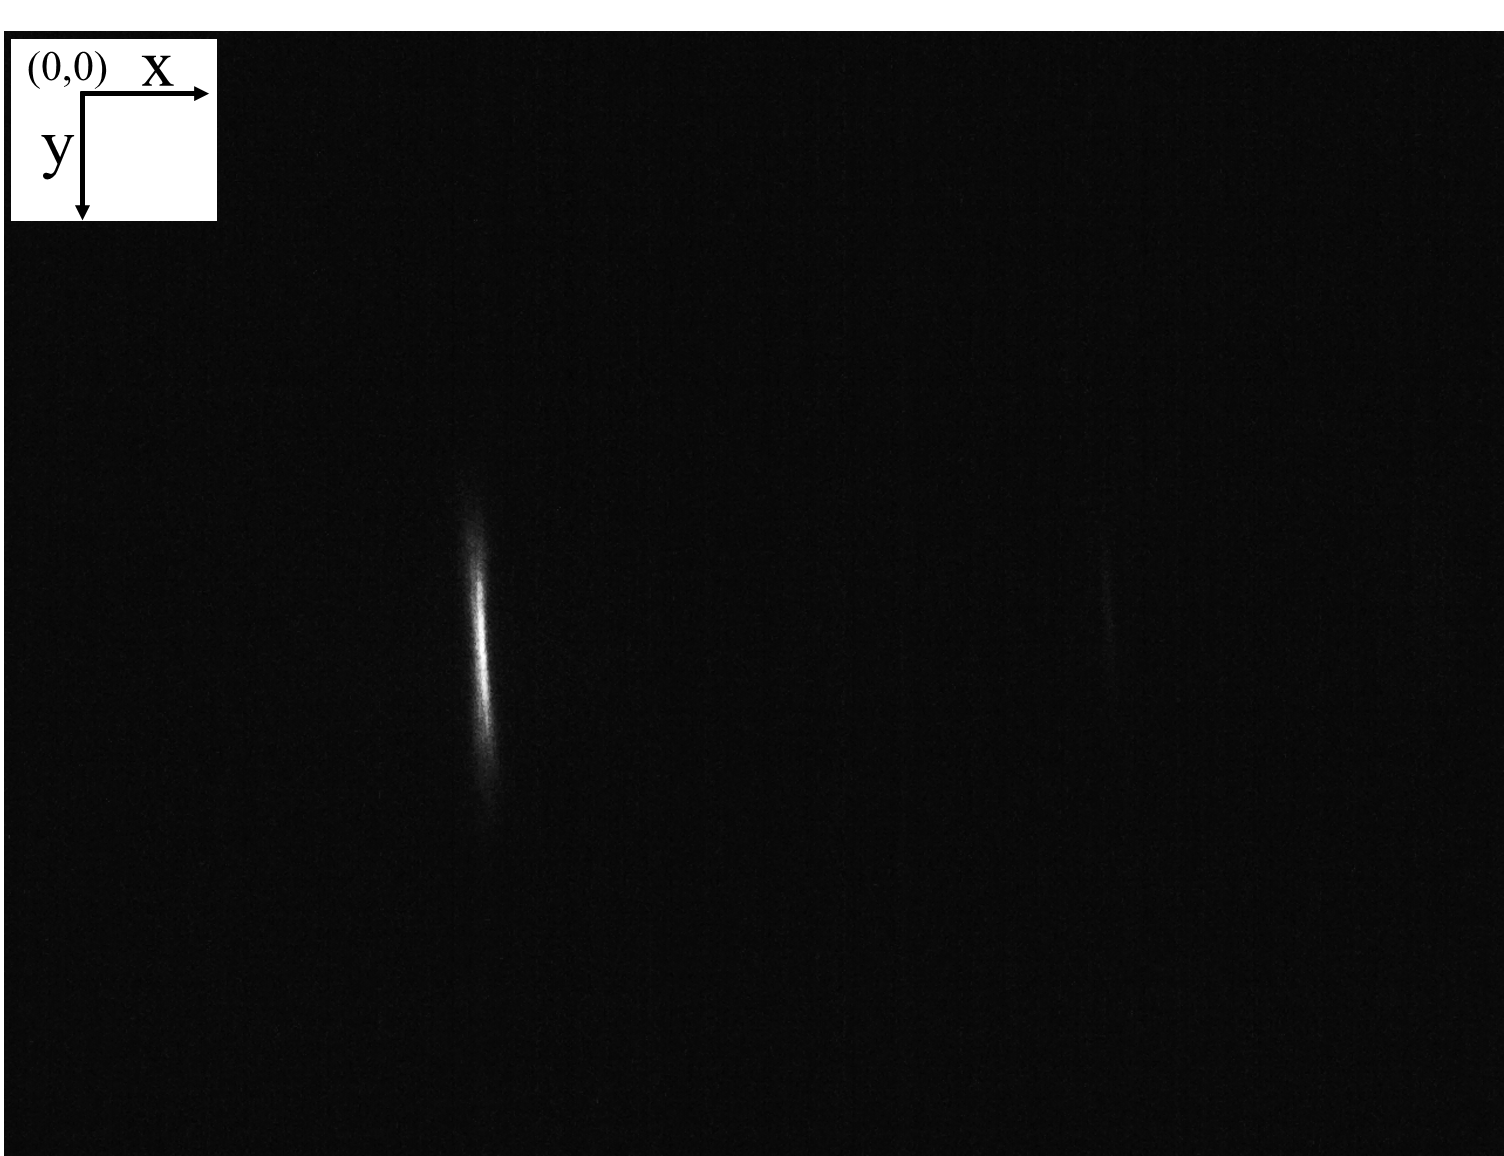
\includegraphics[width=13cm]{figures/TEST_0303_Image__Laser2_2021-03-03-14-23-20.png} %插入图片,[]中设置图片大小,{}中是图片文件名
	\caption{全幅雷射光譜影像} %最终文档中希望显示的图片标题
	\label{全幅雷射光譜影像} %用于文内引用的标签
\end{figure}
若將圖\ref{全幅雷射光譜影像}. 每一個像素皆轉換成光譜訊息,將需要大量的運算,並且在感測器發生漏光(圖\ref{漏光光譜影像}. )時,將會造成光譜波形起始處因漏光而波形失真(圖\ref{漏光時全幅影像光譜波形圖}. ),因此需先由3.3章ROI Scan方式找出全幅影像的ROI區間(圖\ref{全幅雷射ROI光譜影像}. ),以大幅降低運算量,且降低漏光等環境光因素造成的影響。
\begin{figure}[H] %H为当前位置,!htb为忽略美学标准,htbp为浮动图形
	\centering %图片居中
	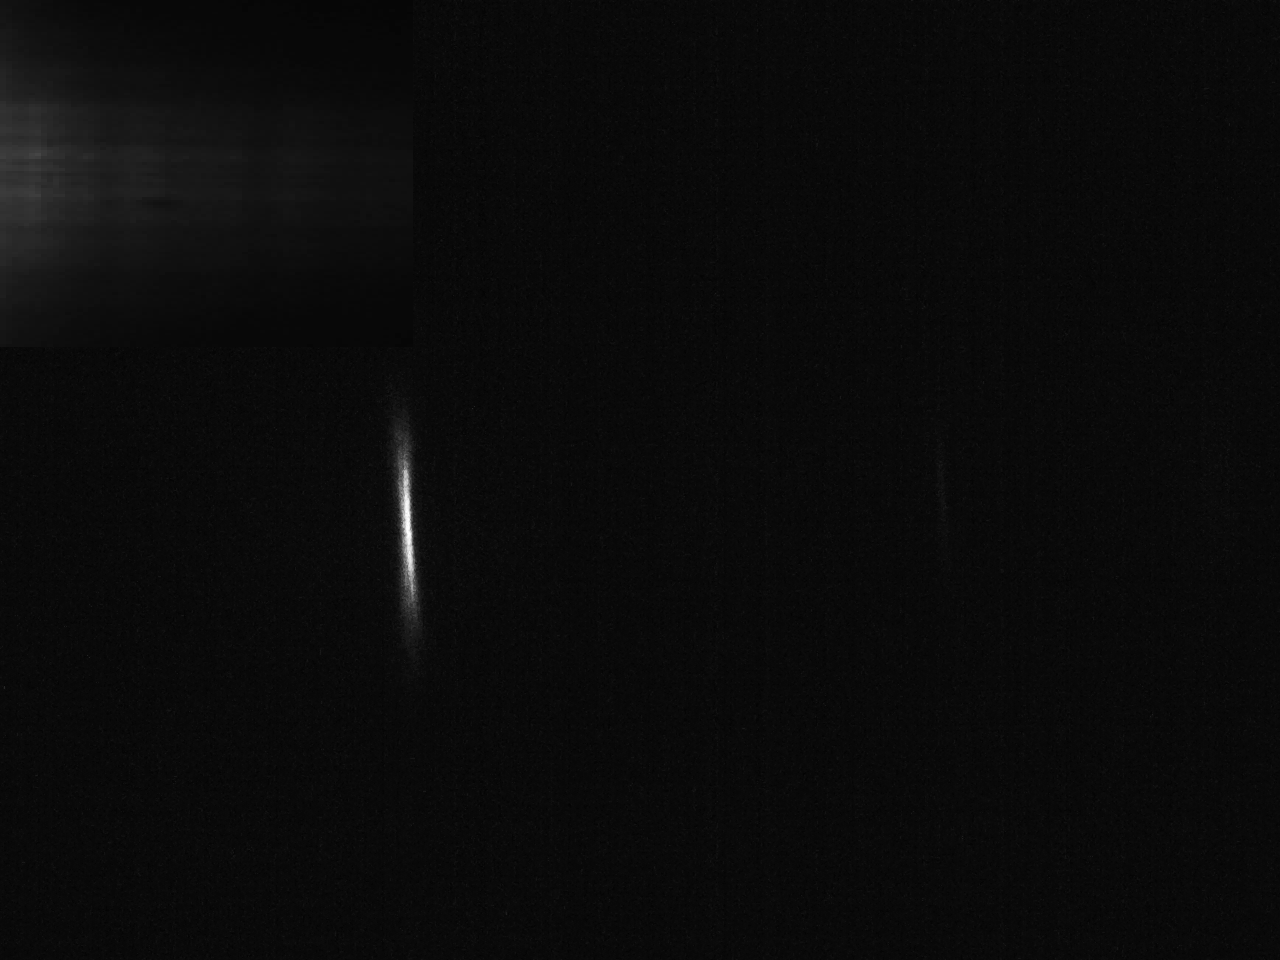
\includegraphics[width=13cm]{figures/漏光影像.png} %插入图片,[]中设置图片大小,{}中是图片文件名
	\caption{漏光光譜影像} %最终文档中希望显示的图片标题
	\label{漏光光譜影像} %用于文内引用的标签
\end{figure}
\begin{figure}[H] %H为当前位置,!htb为忽略美学标准,htbp为浮动图形
	\centering %图片居中
	\setlength{\abovecaptionskip}{0.cm}
	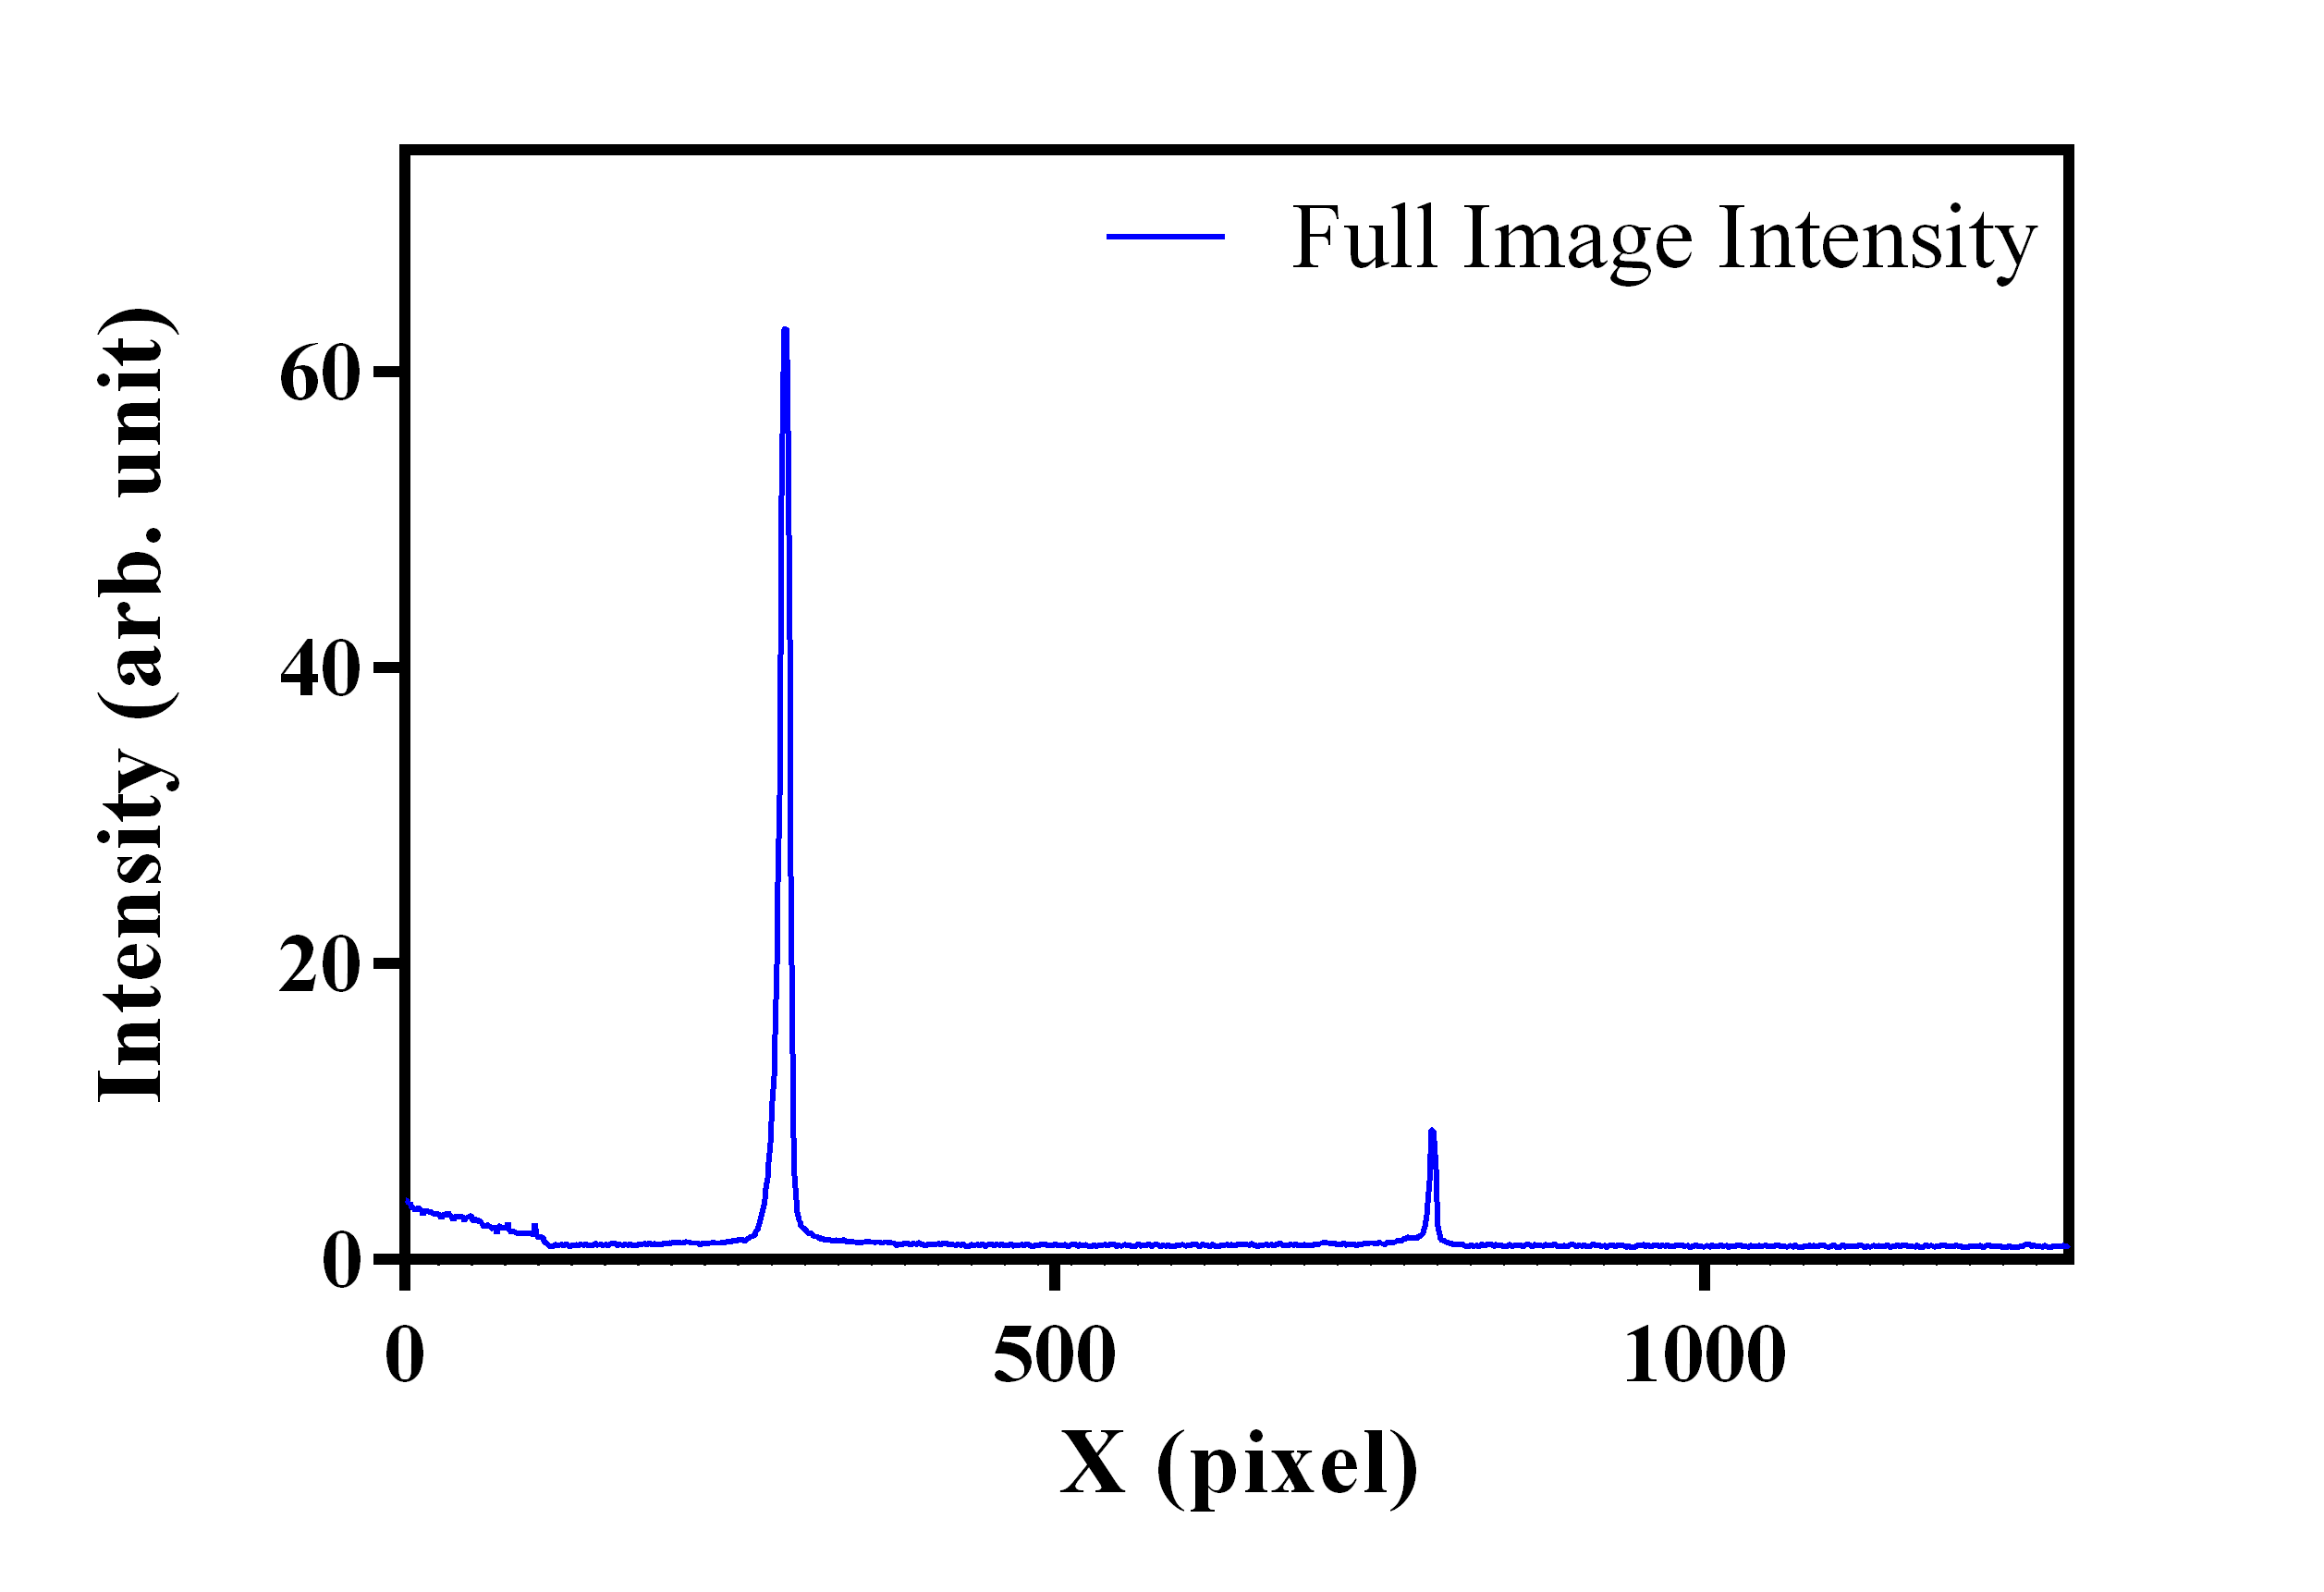
\includegraphics[width=15cm]{figures/MissLight.png} %插入图片,[]中设置图片大小,{}中是图片文件名
	\caption{漏光時全幅影像光譜波形圖} %最终文档中希望显示的图片标题
	\label{漏光時全幅影像光譜波形圖} %用于文内引用的标签
\end{figure}
\begin{figure}[H] %H为当前位置,!htb为忽略美学标准,htbp为浮动图形
	\centering %图片居中
	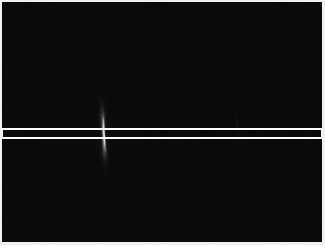
\includegraphics[width=10cm]{figures/TEST_0303_full_Image__Laser2_2021-03-03-14-23.jpg} %插入图片,[]中设置图片大小,{}中是图片文件名
	\caption{全幅雷射ROI光譜影像} %最终文档中希望显示的图片标题
	\label{全幅雷射ROI光譜影像} %用于文内引用的标签
\end{figure}
得出ROI區域後,將ROI區間的影像由全幅雷射光譜影像中單獨取出分析,如圖\ref{ROI光譜影像}. 所示。
\begin{figure}[H] %H为当前位置,!htb为忽略美学标准,htbp为浮动图形
	\centering %图片居中
	\vspace{0.8cm}
	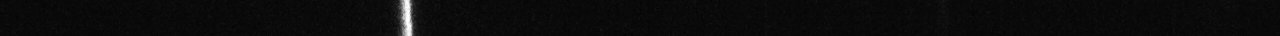
\includegraphics[width=13cm]{figures/TEST_0303_ROI__Laser2_2021-03-03-14-23-20.jpg} %插入图片,[]中设置图片大小,{}中是图片文件名
	\caption{ROI光譜影像} %最终文档中希望显示的图片标题
	\label{ROI光譜影像} %用于文内引用的标签
\end{figure}
影像感測器所取出之原始光譜影像為三通道RGB影像,透過2.1章的RBG轉換式(\ref{eq:2.4})將ROI光譜影像中每一個像素的RGB值,透過灰度轉換公式轉換成灰度值,比如影像在$Pixel(400,520)$位置的RGB值為$(174,156,148)$,以$RGB(400,520)=(174,156,148)$表示並帶入式(\ref{eq:2.4})。
\begin{equation}
	Gray(400,520) = (174\times313524 + 156\times615514 + 148\times119538) >> 20
	\label{RGB:3.3}
\end{equation}
其中$Gray(400,520)$為在$Pixel(400,520)$的灰度值表示,計算後為
\begin{equation}
	Gray(400,520) = 168264984_{(10)} >> 20
	\label{RGB:3.4}
\end{equation}
再將十進制灰度值轉換為二進制
\begin{equation}
	Gray(400,520) = 1010000001111000010100011000_{(2)} >> 20
	\label{RGB:3.5}
\end{equation}
再對二進制灰度值像右位移20個位元,得
\begin{equation}
	Gray(400,520) = 10100000_{(2)}
	\label{RGB:3.6}
\end{equation}
最後轉回十進制
\begin{equation}
	Gray(400,520) = 160_{(10)}
	\label{RGB:3.7}
\end{equation}
將ROI中所有像素如式(\ref{RGB:3.3})至式(\ref{RGB:3.7})逐一帶入,則得出影像每一像素之灰度值,將ROI影像以灰度值矩陣表示。
\begin{equation}\label{RGB:3.8}
	\begin{bmatrix} 
		G(0,0)&G(1,0)&\cdots&G(1278,0)&G(1279,0)\\
		G(0,1)&G(1,1)&\cdots&G(1278,1)&G(1279,1)\\
		\vdots&\vdots&\ddots&\vdots&\vdots\\
		G(0,18)&G(1,18)&\cdots&G(1278,18)&G(1279,18)\\
		G(0,19)&G(1,19)&\cdots&G(1279,19)&G(1279,19)\\
	\end{bmatrix}_{20\times1280}
\end{equation}
矩陣對每一行各自取灰度值平均,則得出像素對光度數據矩陣。
\begin{equation}\label{RGB:3.9}
	\begin{bmatrix} 
		\frac{\Sigma_{i=0}^{i=19}G(0,i)}{20}&\frac{\Sigma_{i=0}^{i=19}G(1,i)}{20}&\cdots&\frac{\Sigma_{i=0}^{i=19}G(1278,i)}{20}&\frac{\Sigma_{i=0}^{i=19}G(1279,i)}{20}\\
	\end{bmatrix}_{1\times1280}
\end{equation}
式(\ref{RGB:3.9})中$1\times1280$之矩陣即為光譜數據矩陣,其中每一像素對應一個光度值,轉換完成後的光譜波形圖如圖\ref{ROI光譜強度圖}. 所示。
\begin{figure}[H] %H为当前位置,!htb为忽略美学标准,htbp为浮动图形
	\centering %图片居中
	\setlength{\abovecaptionskip}{0.cm}
	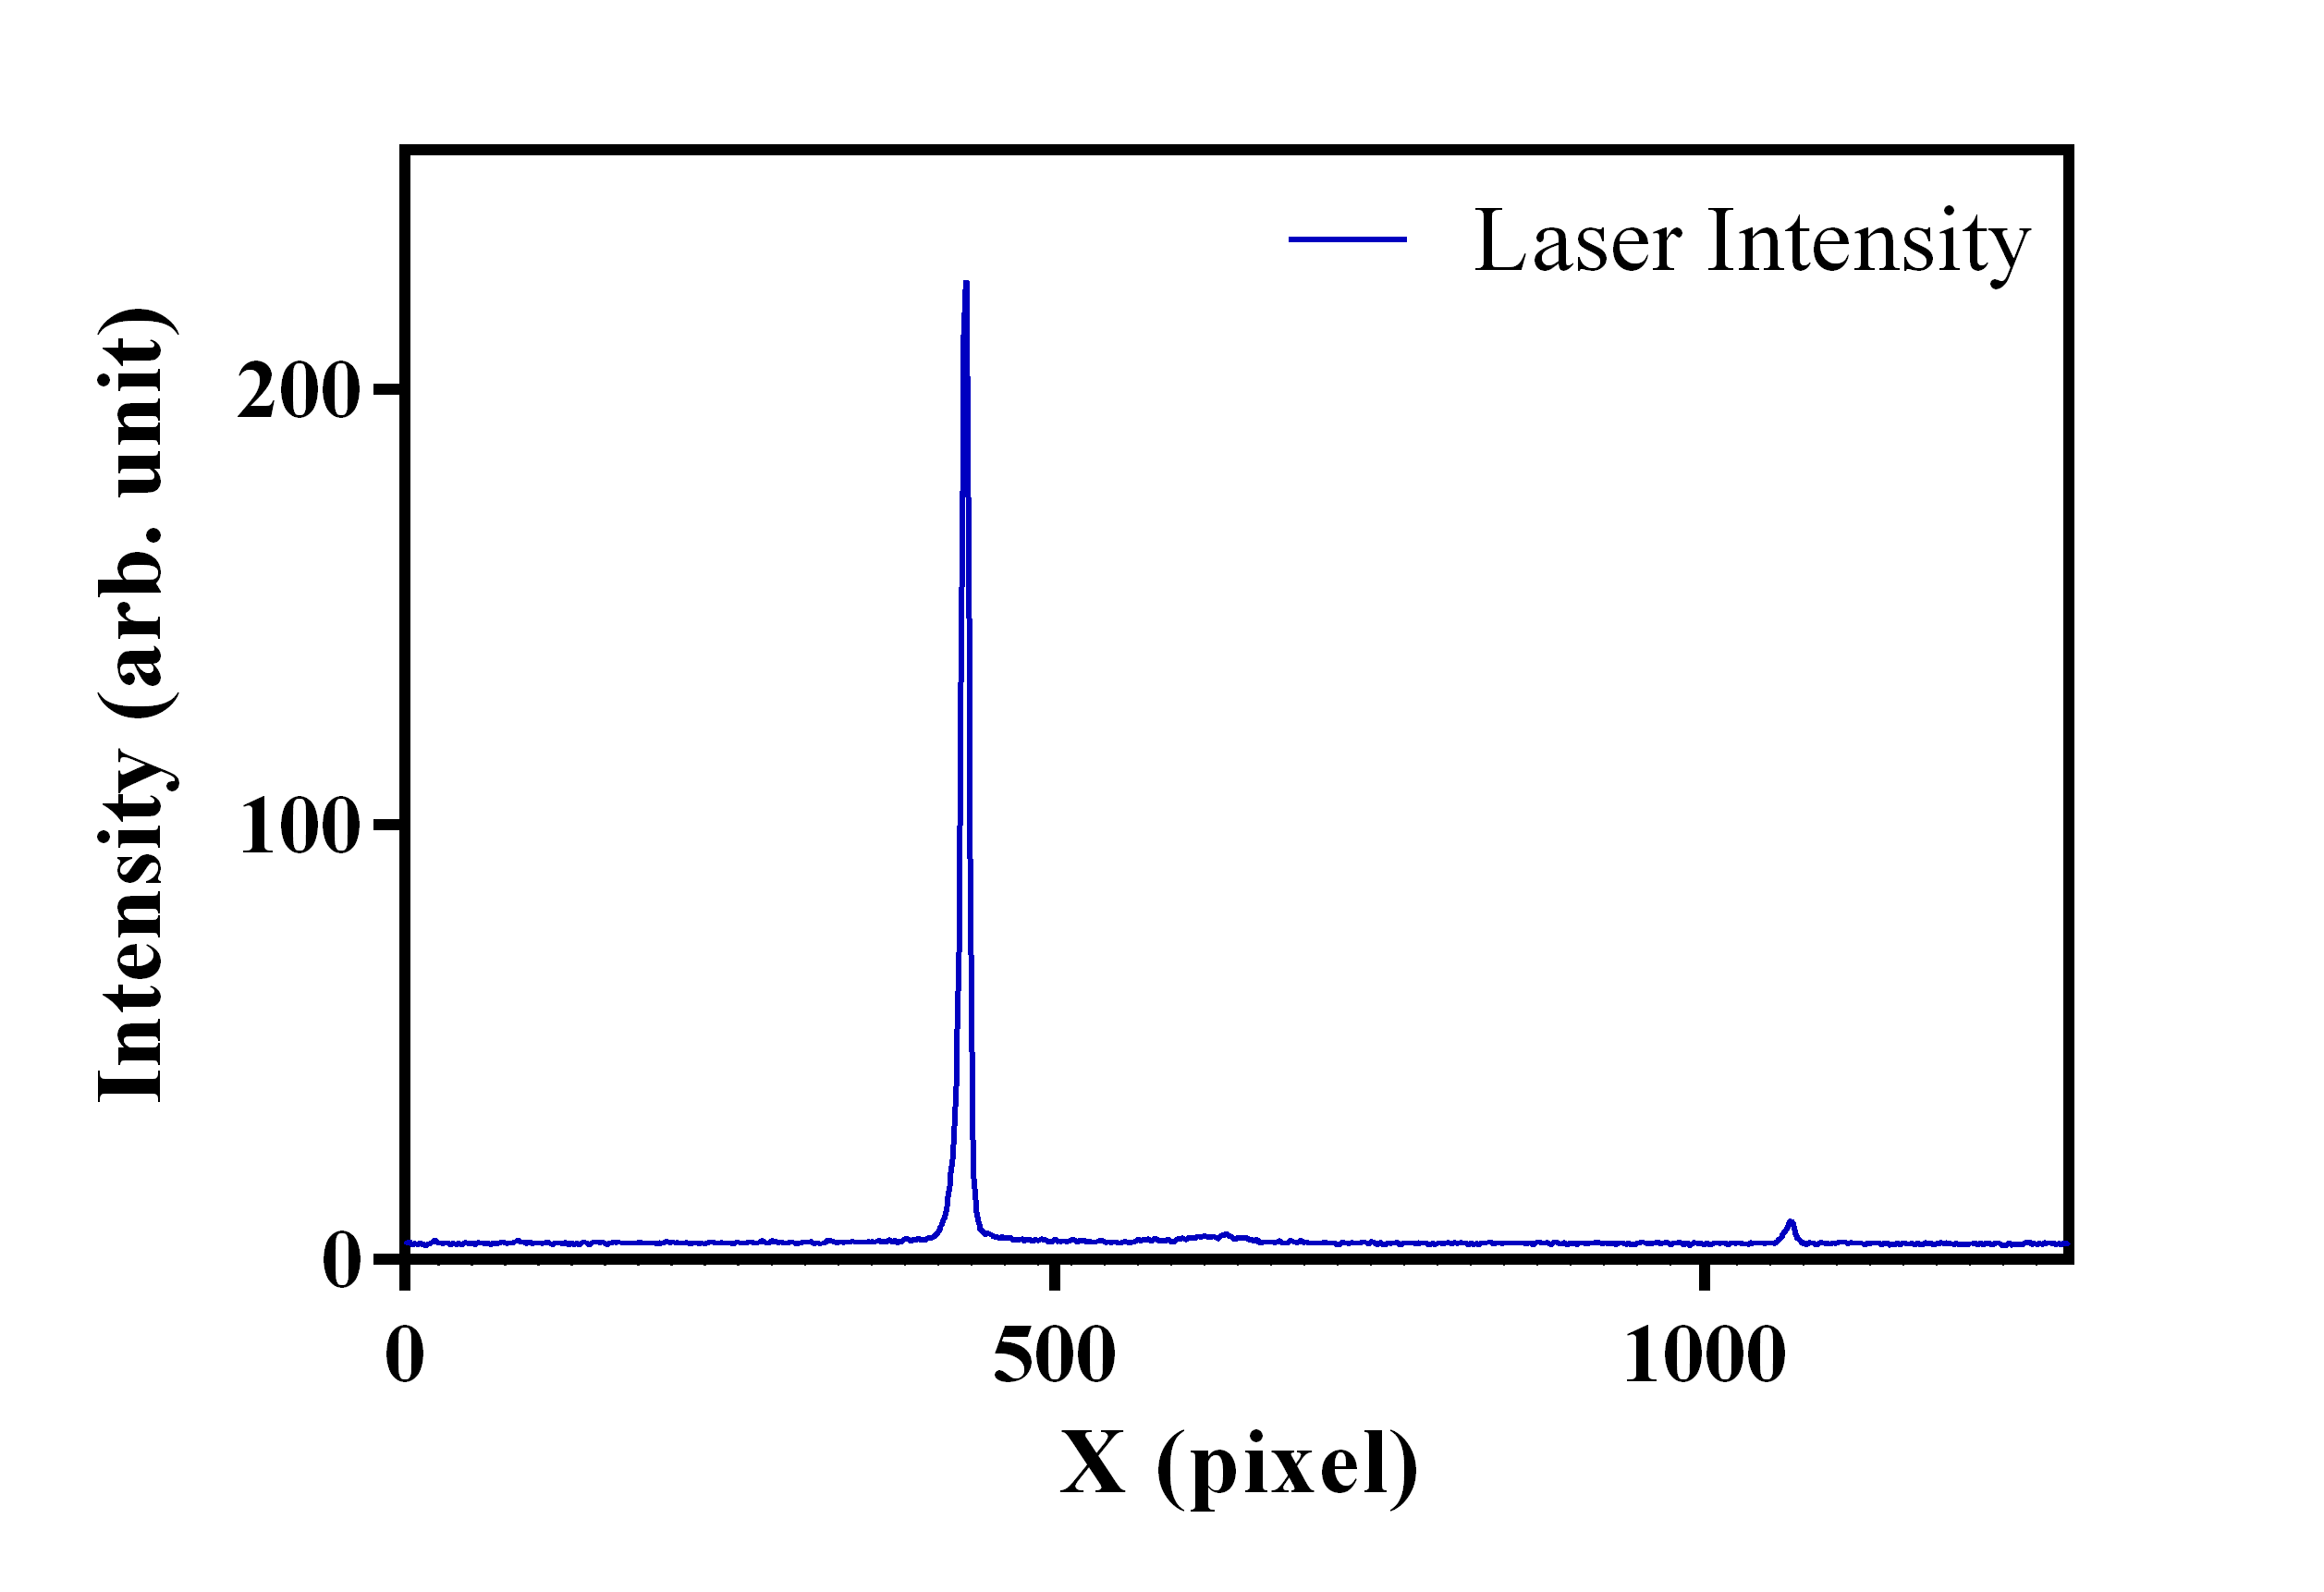
\includegraphics[width=\textwidth]{figures/Laser_Intensity.PNG} %插入图片,[]中设置图片大小,{}中是图片文件名
	\caption{ROI光譜強度圖} %最终文档中希望显示的图片标题
	\label{ROI光譜強度圖} %用于文内引用的标签
\end{figure}
\section{Auto Scaling}
取得光譜波形資訊後,並無法立即進行分析,因受限於灰度強度最高值255,當光線強度過強而超出255時即稱為過瞨\cite{over-exposure},光譜過曝如圖\ref{白光光譜過瞨圖}. 所示,波峰位置將難以辨認,因此需調低影像感測器參數,以獲得較低的光譜影像,直至總光譜的最大強度值達到目標強度為止,而當輸入波形因晶片效率較差或光源較暗,而導致強度過低如圖\ref{白光光譜強度過低圖}. 所示,則需調高影像感測器參數,直至獲得強度為目標強度為止,而上述步驟統稱為Auto Scaling,Auto Scaling結束的光譜波形表現如圖\ref{白光光譜經Auto Scaling後光譜波形表現}. 所示,強度調整至約由使用者設定的255的90\%,此光譜波形將比起未Auto Scaling來的容易分析許多。
\newpage
\begin{figure}[H] %H为当前位置,!htb为忽略美学标准,htbp为浮动图形
	\centering %图片居中
	\setlength{\abovecaptionskip}{0.cm}
	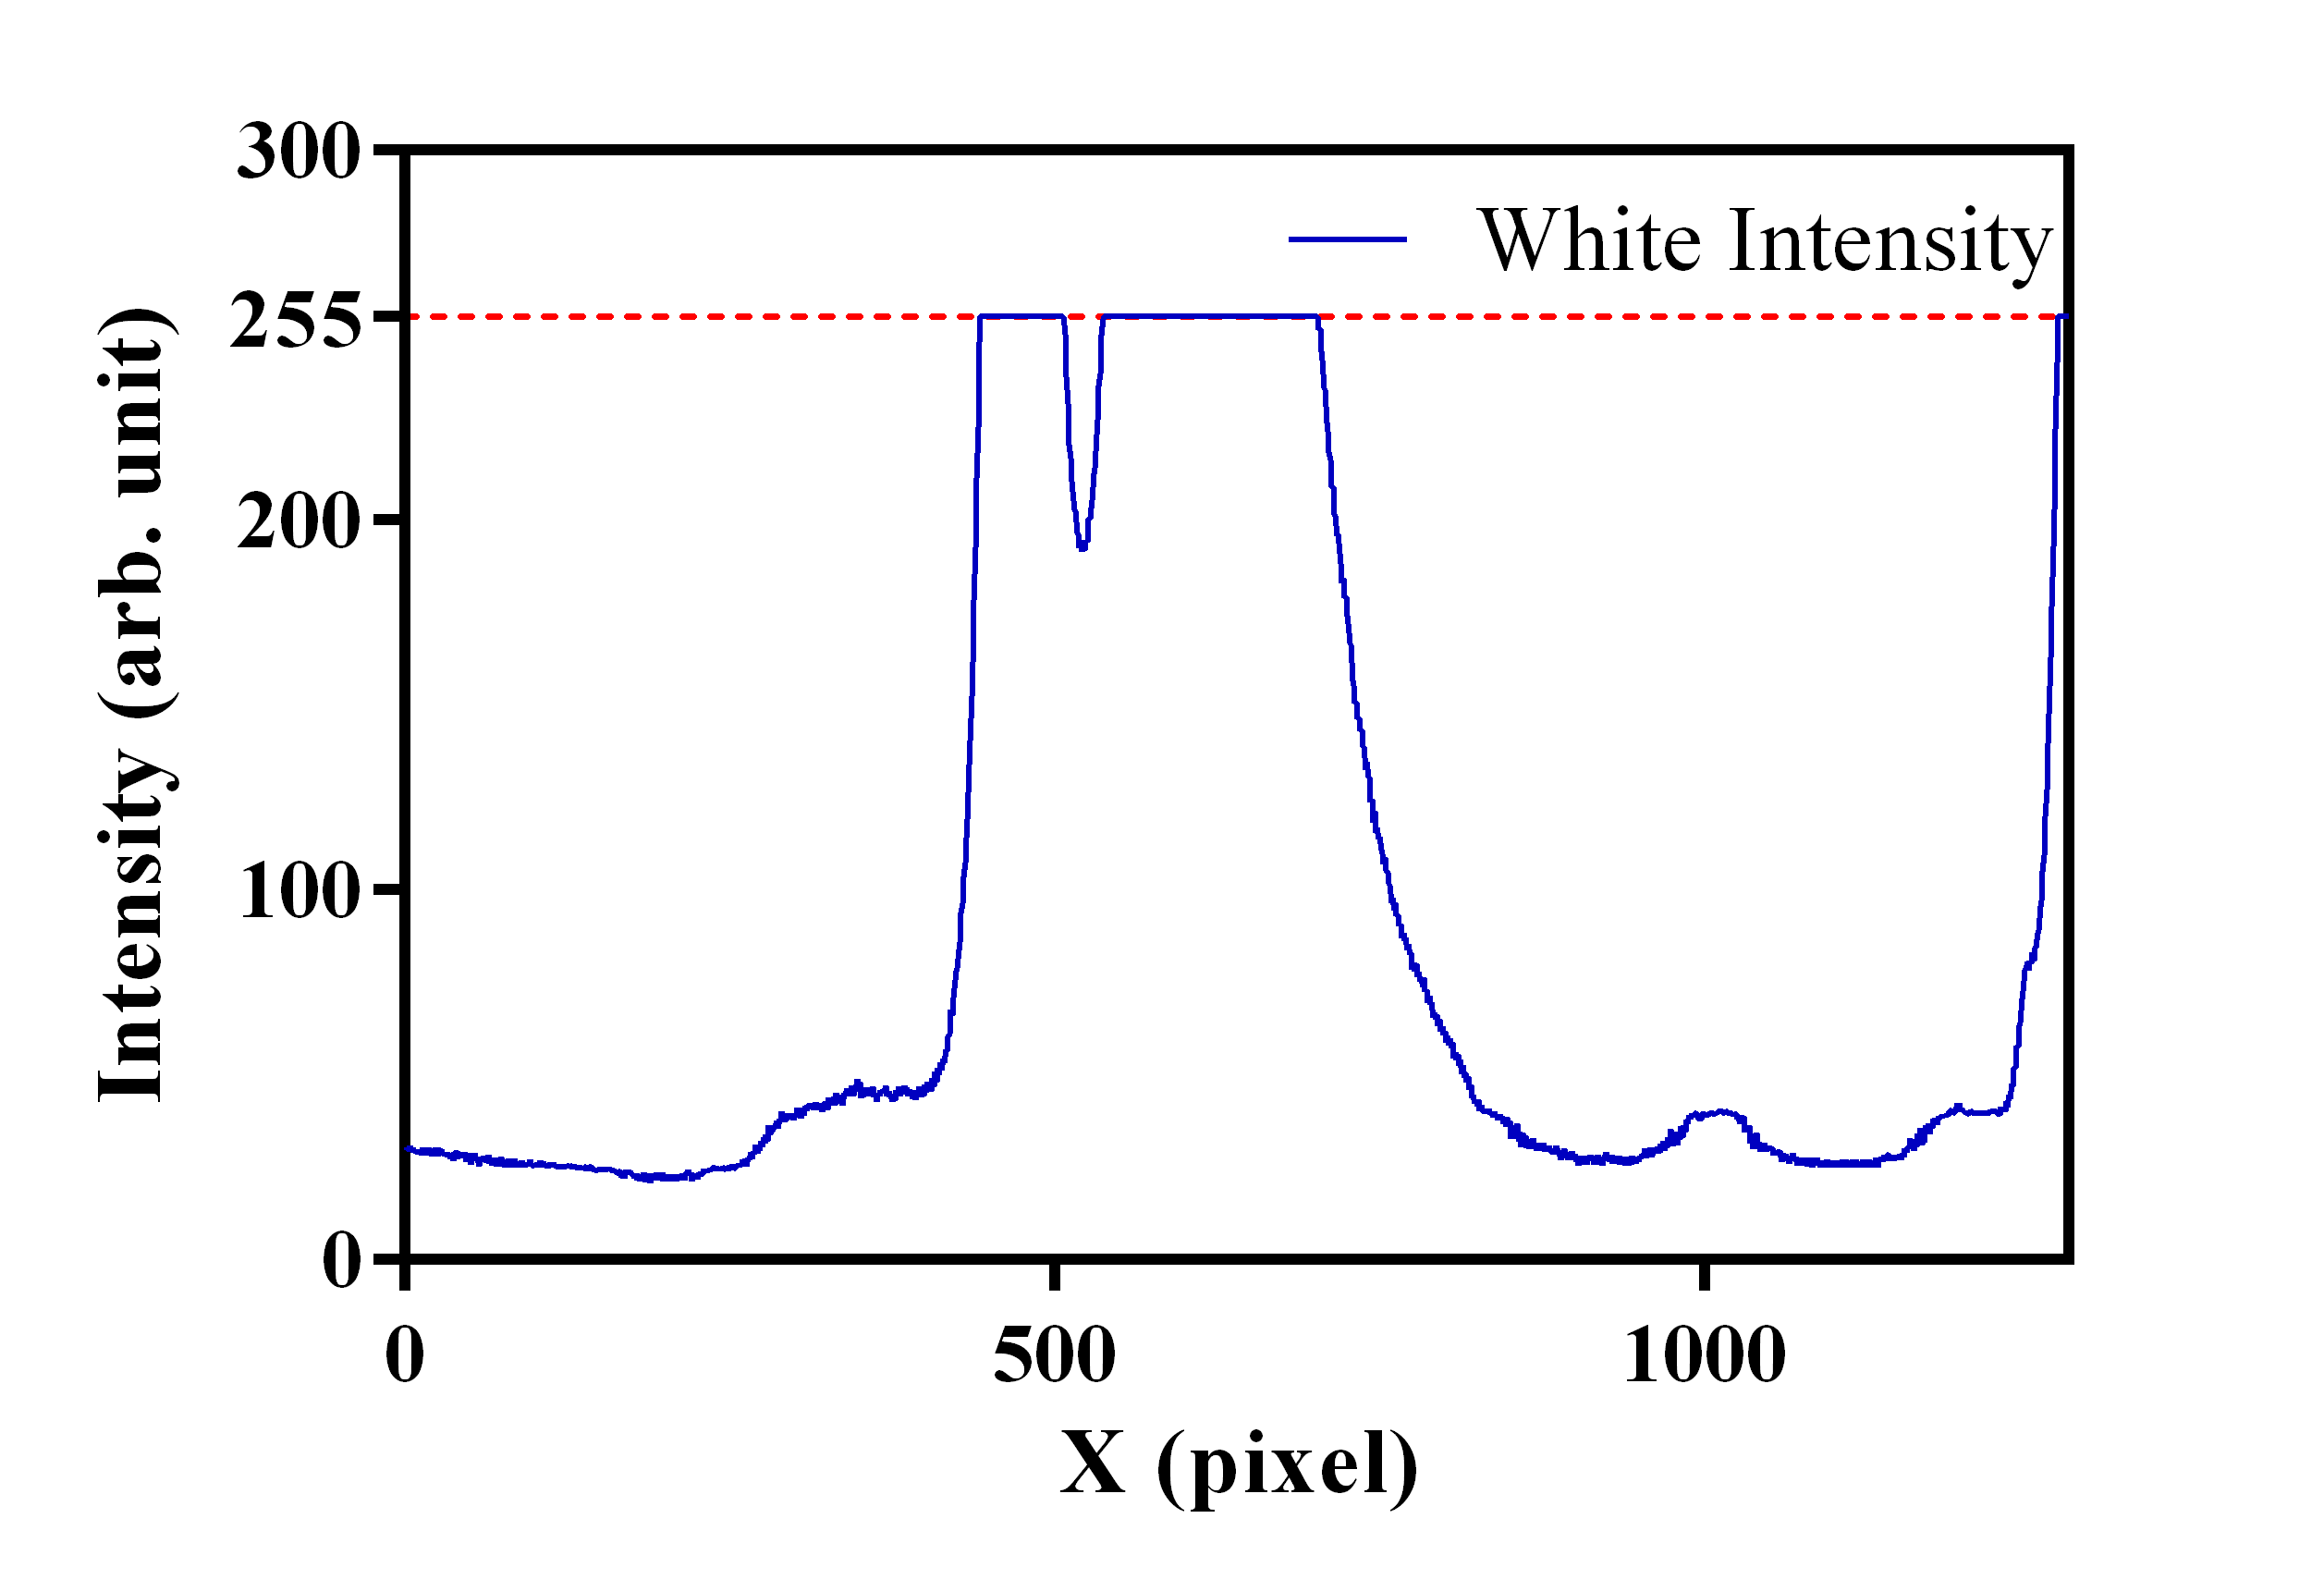
\includegraphics[width=\textwidth]{figures/White_Over.PNG} %插入图片,[]中设置图片大小,{}中是图片文件名
	\caption{白光光譜過瞨圖} %最终文档中希望显示的图片标题
	\label{白光光譜過瞨圖} %用于文内引用的标签
\end{figure}
\begin{figure}[H] %H为当前位置,!htb为忽略美学标准,htbp为浮动图形
	\centering %图片居中
	\setlength{\belowcaptionskip}{-1cm} 
	\setlength{\abovecaptionskip}{0.cm}
	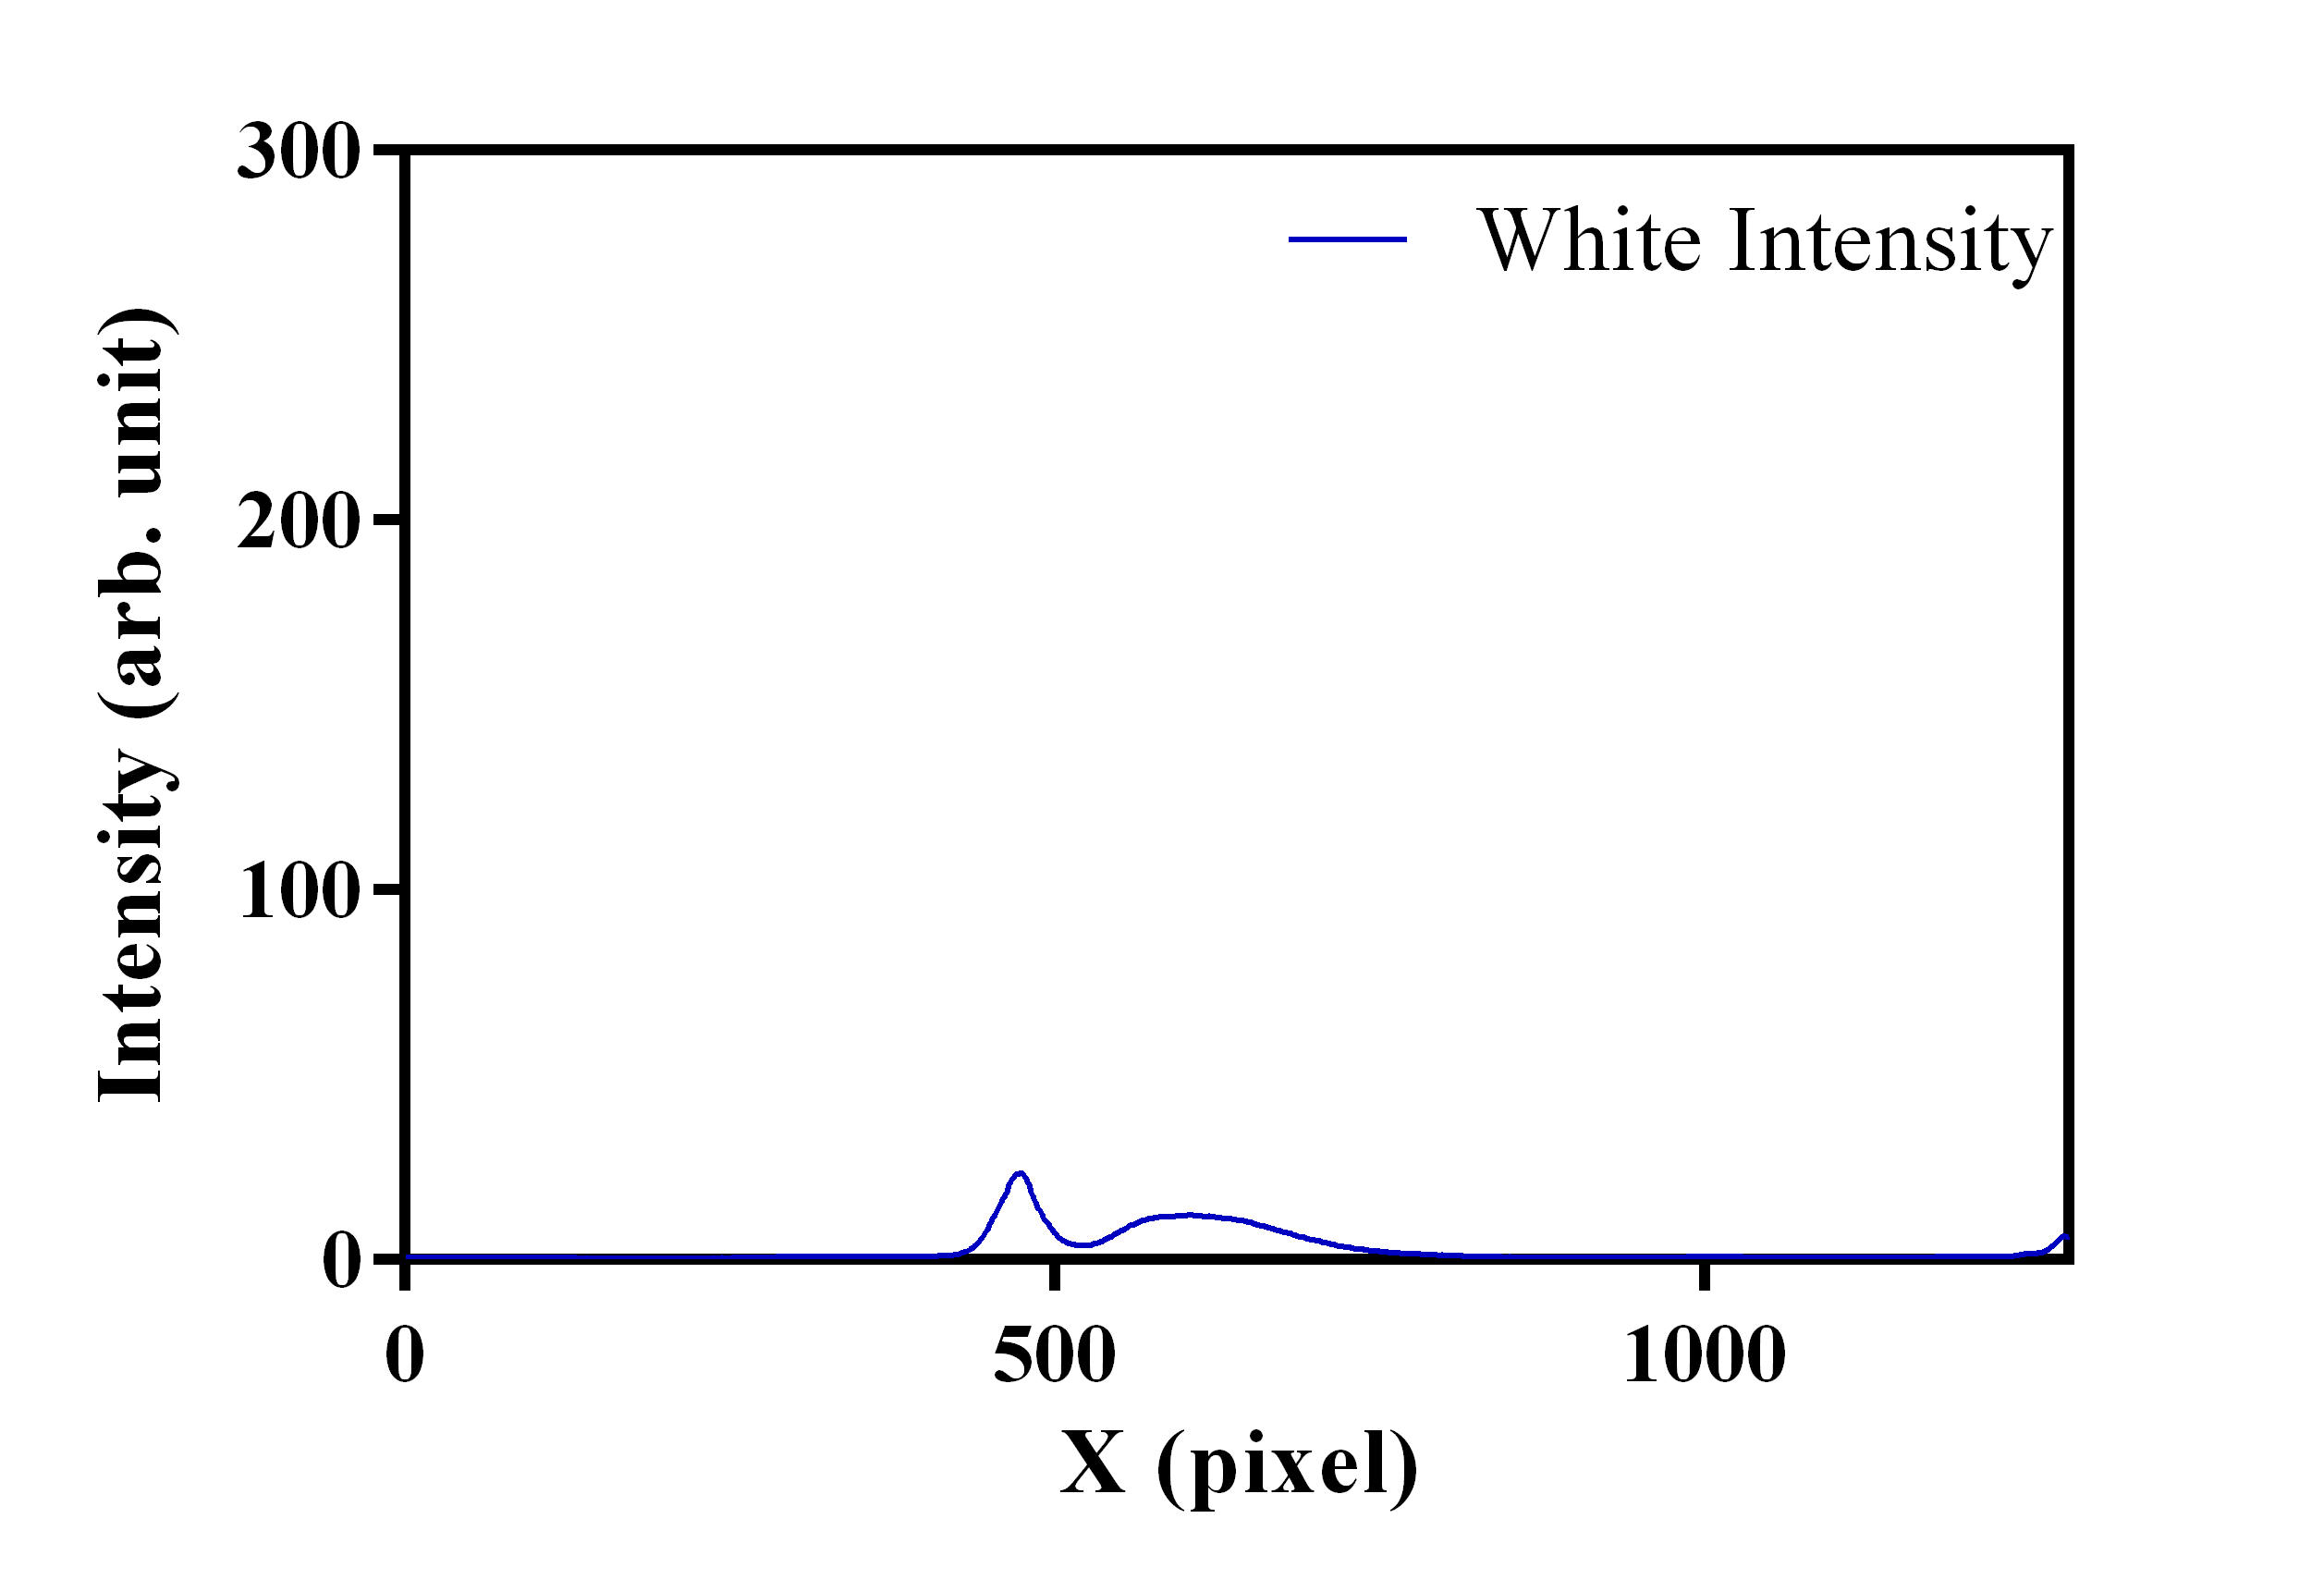
\includegraphics[width=\textwidth]{figures/White_weak.PNG} %插入图片,[]中设置图片大小,{}中是图片文件名
	\caption{白光光譜強度過低圖} %最终文档中希望显示的图片标题
	\label{白光光譜強度過低圖} %用于文内引用的标签
\end{figure}\newpage
\begin{figure}[H] %H为当前位置,!htb为忽略美学标准,htbp为浮动图形
	\centering %图片居中
	\setlength{\abovecaptionskip}{0.cm}
	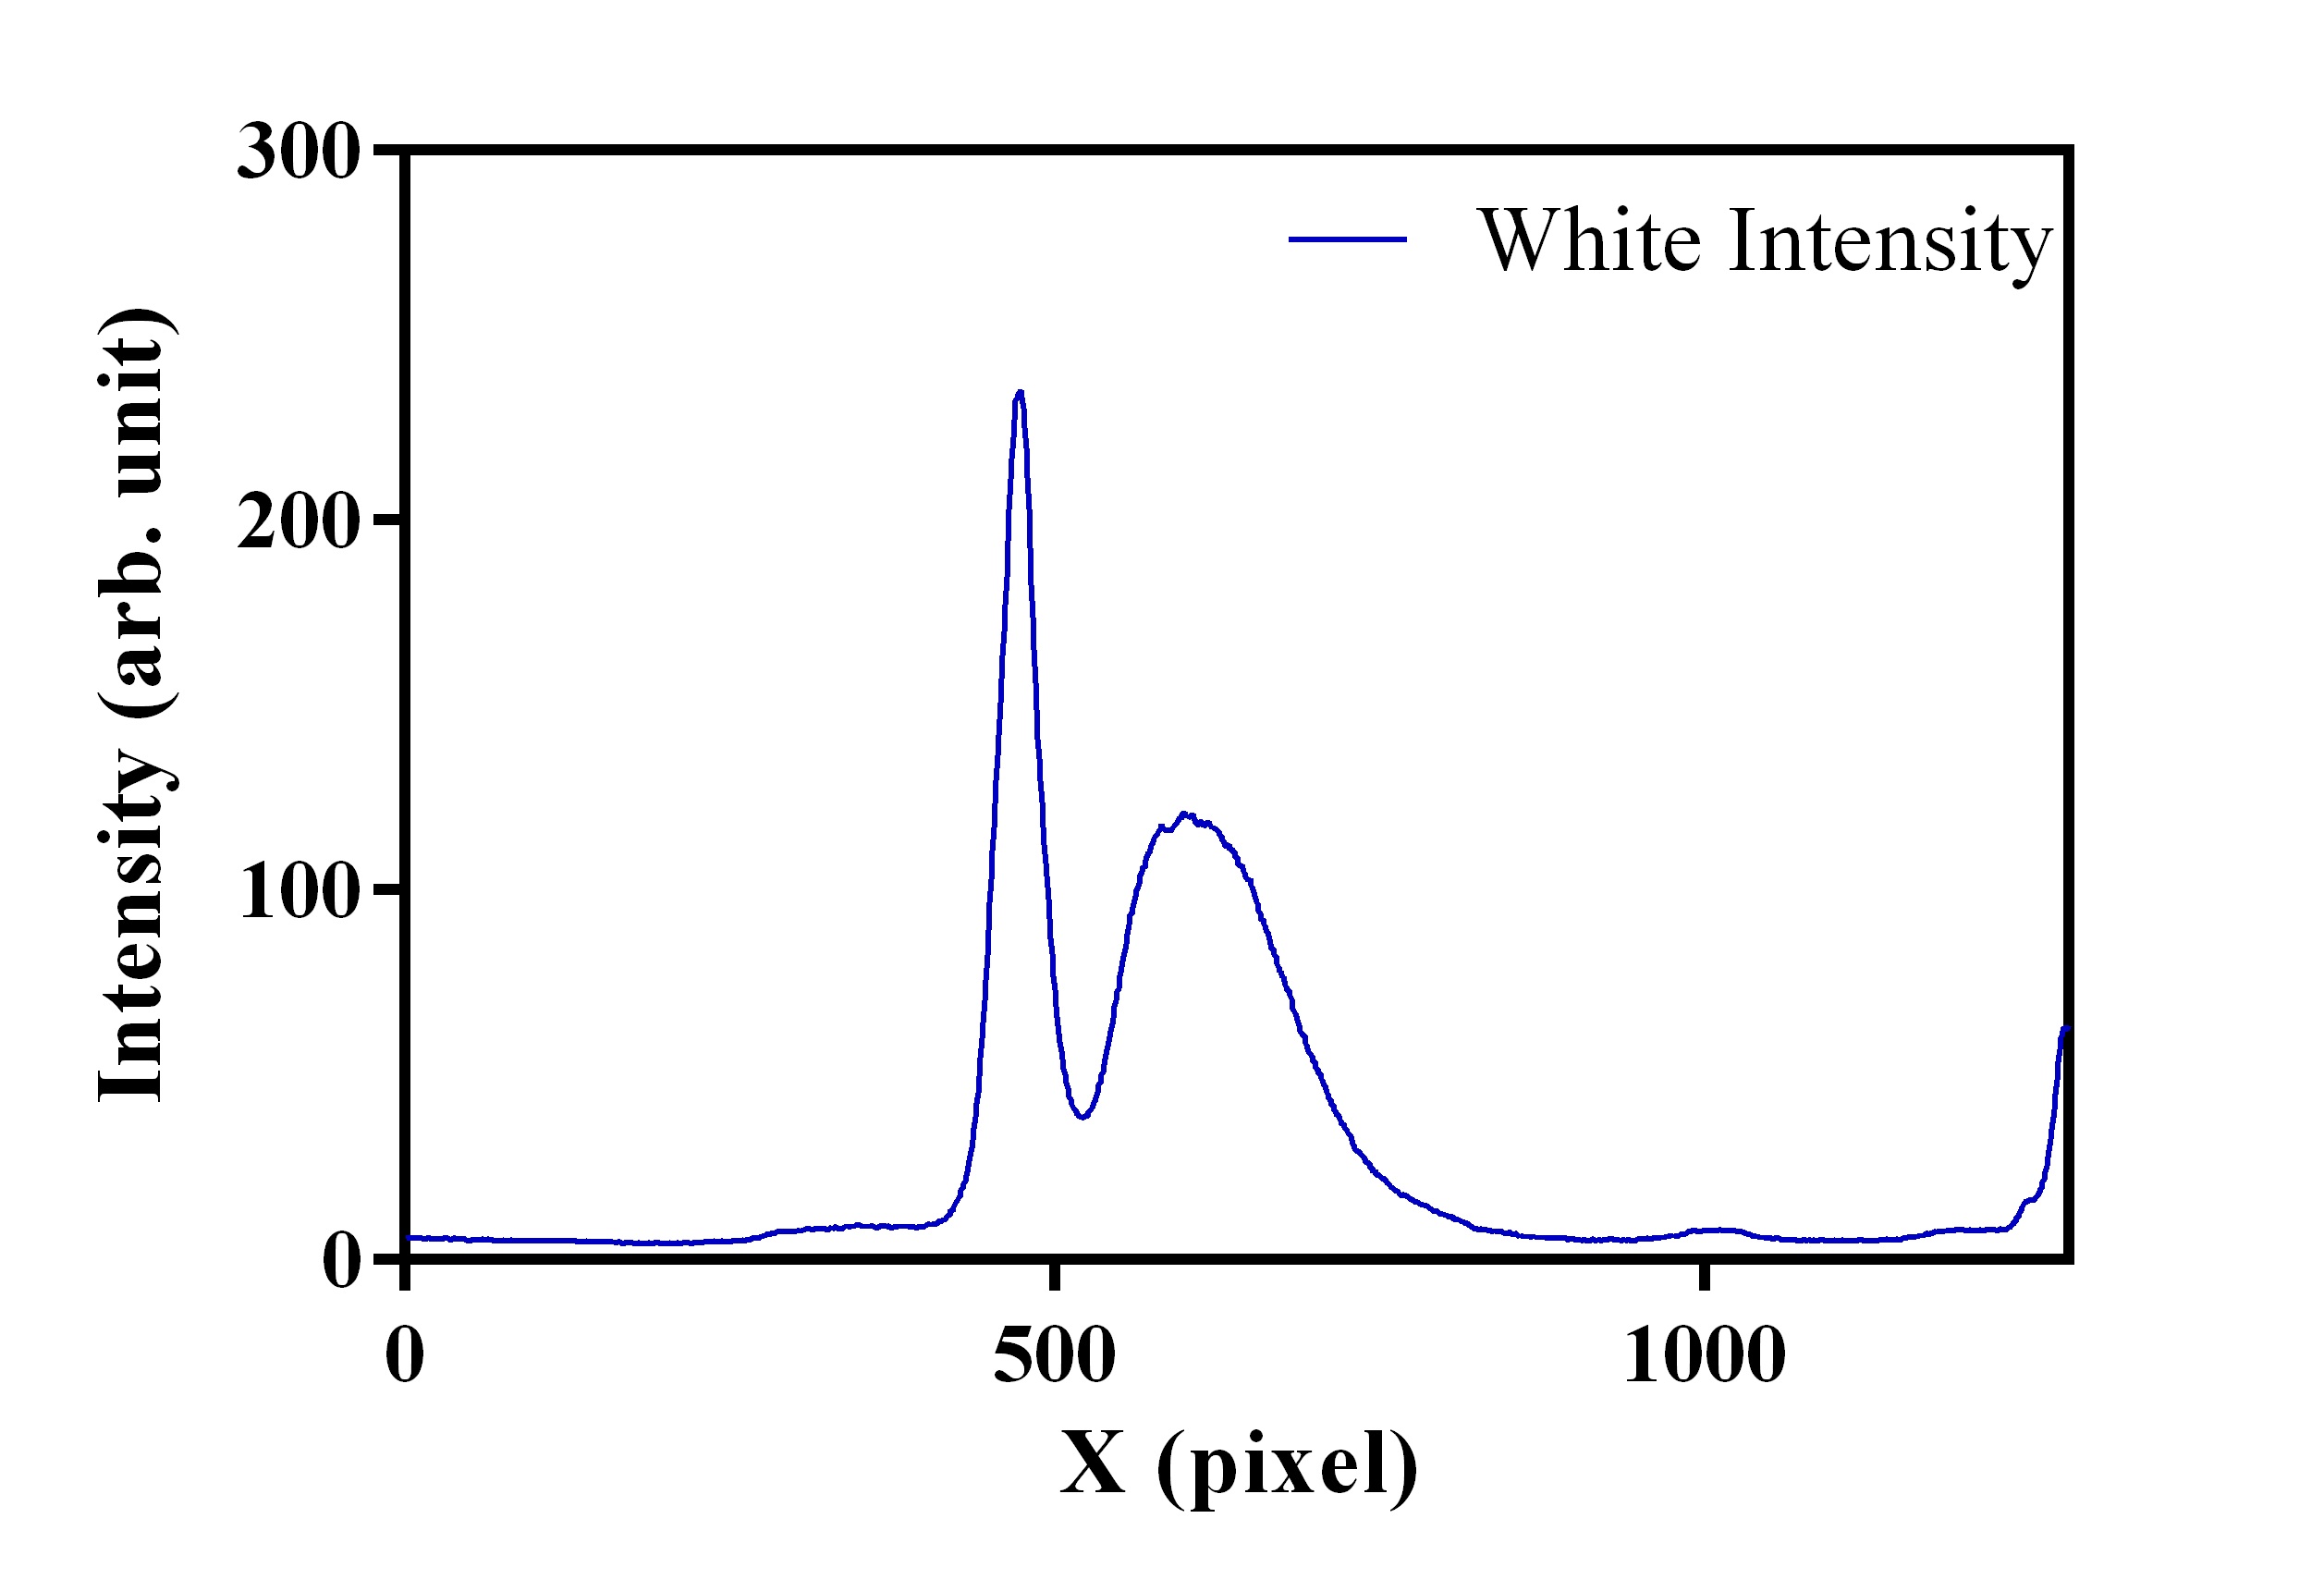
\includegraphics[width=\textwidth]{figures/White_As.PNG} %插入图片,[]中设置图片大小,{}中是图片文件名
	\caption{白光光譜經Auto Scaling後光譜波形表現} %最终文档中希望显示的图片标题
	\label{白光光譜經Auto Scaling後光譜波形表現} %用于文内引用的标签
\end{figure}
\par
但並非所有Auto Scaling都能將光譜調整至指定強度,如同表\ref{峰值位置比較表}. 所示,DG範圍受限在32\textasciitilde255之間,當一輸入光源過低而導致由公式(\ref{eq:2.6})所計算出的$DG_{goal}$超出255,則表示在Gamma = 100、BL = 0的條件下無法達成,因此需要調整其餘兩項參數,而又因Gamma與電雜訊將成正比升高,因此優先考慮調整BL,將BL由0至3階逐步升高,直至計算出的$DG_{goal}$小於255,若BL以達最高值仍然無法使$DG_{goal}$小於255,則將Gamma以每次增加50為一單位逐步提升,直至計算出的$DG_{goal}$小於255,若依然無法達成,僅剩更換較強光源這一選擇。\par
反之,當光源強度過強而導致由公式(\ref{eq:2.6})所計算出的$DG_{goal}$低於32時,由於此時$DG_{goal}$是以Gamma = 100、BL = 0的條件下所計算出,因此所有可調參數皆以達最低值,此時僅剩更換較低光源此一選項。所有Auto Scaling完整流程如圖\ref{Auto Scaling流程圖}. 所示。
\newpage
\begin{figure}[H] %H为当前位置,!htb为忽略美学标准,htbp为浮动图形
	\centering %图片居中
	\setlength{\abovecaptionskip}{1cm}
	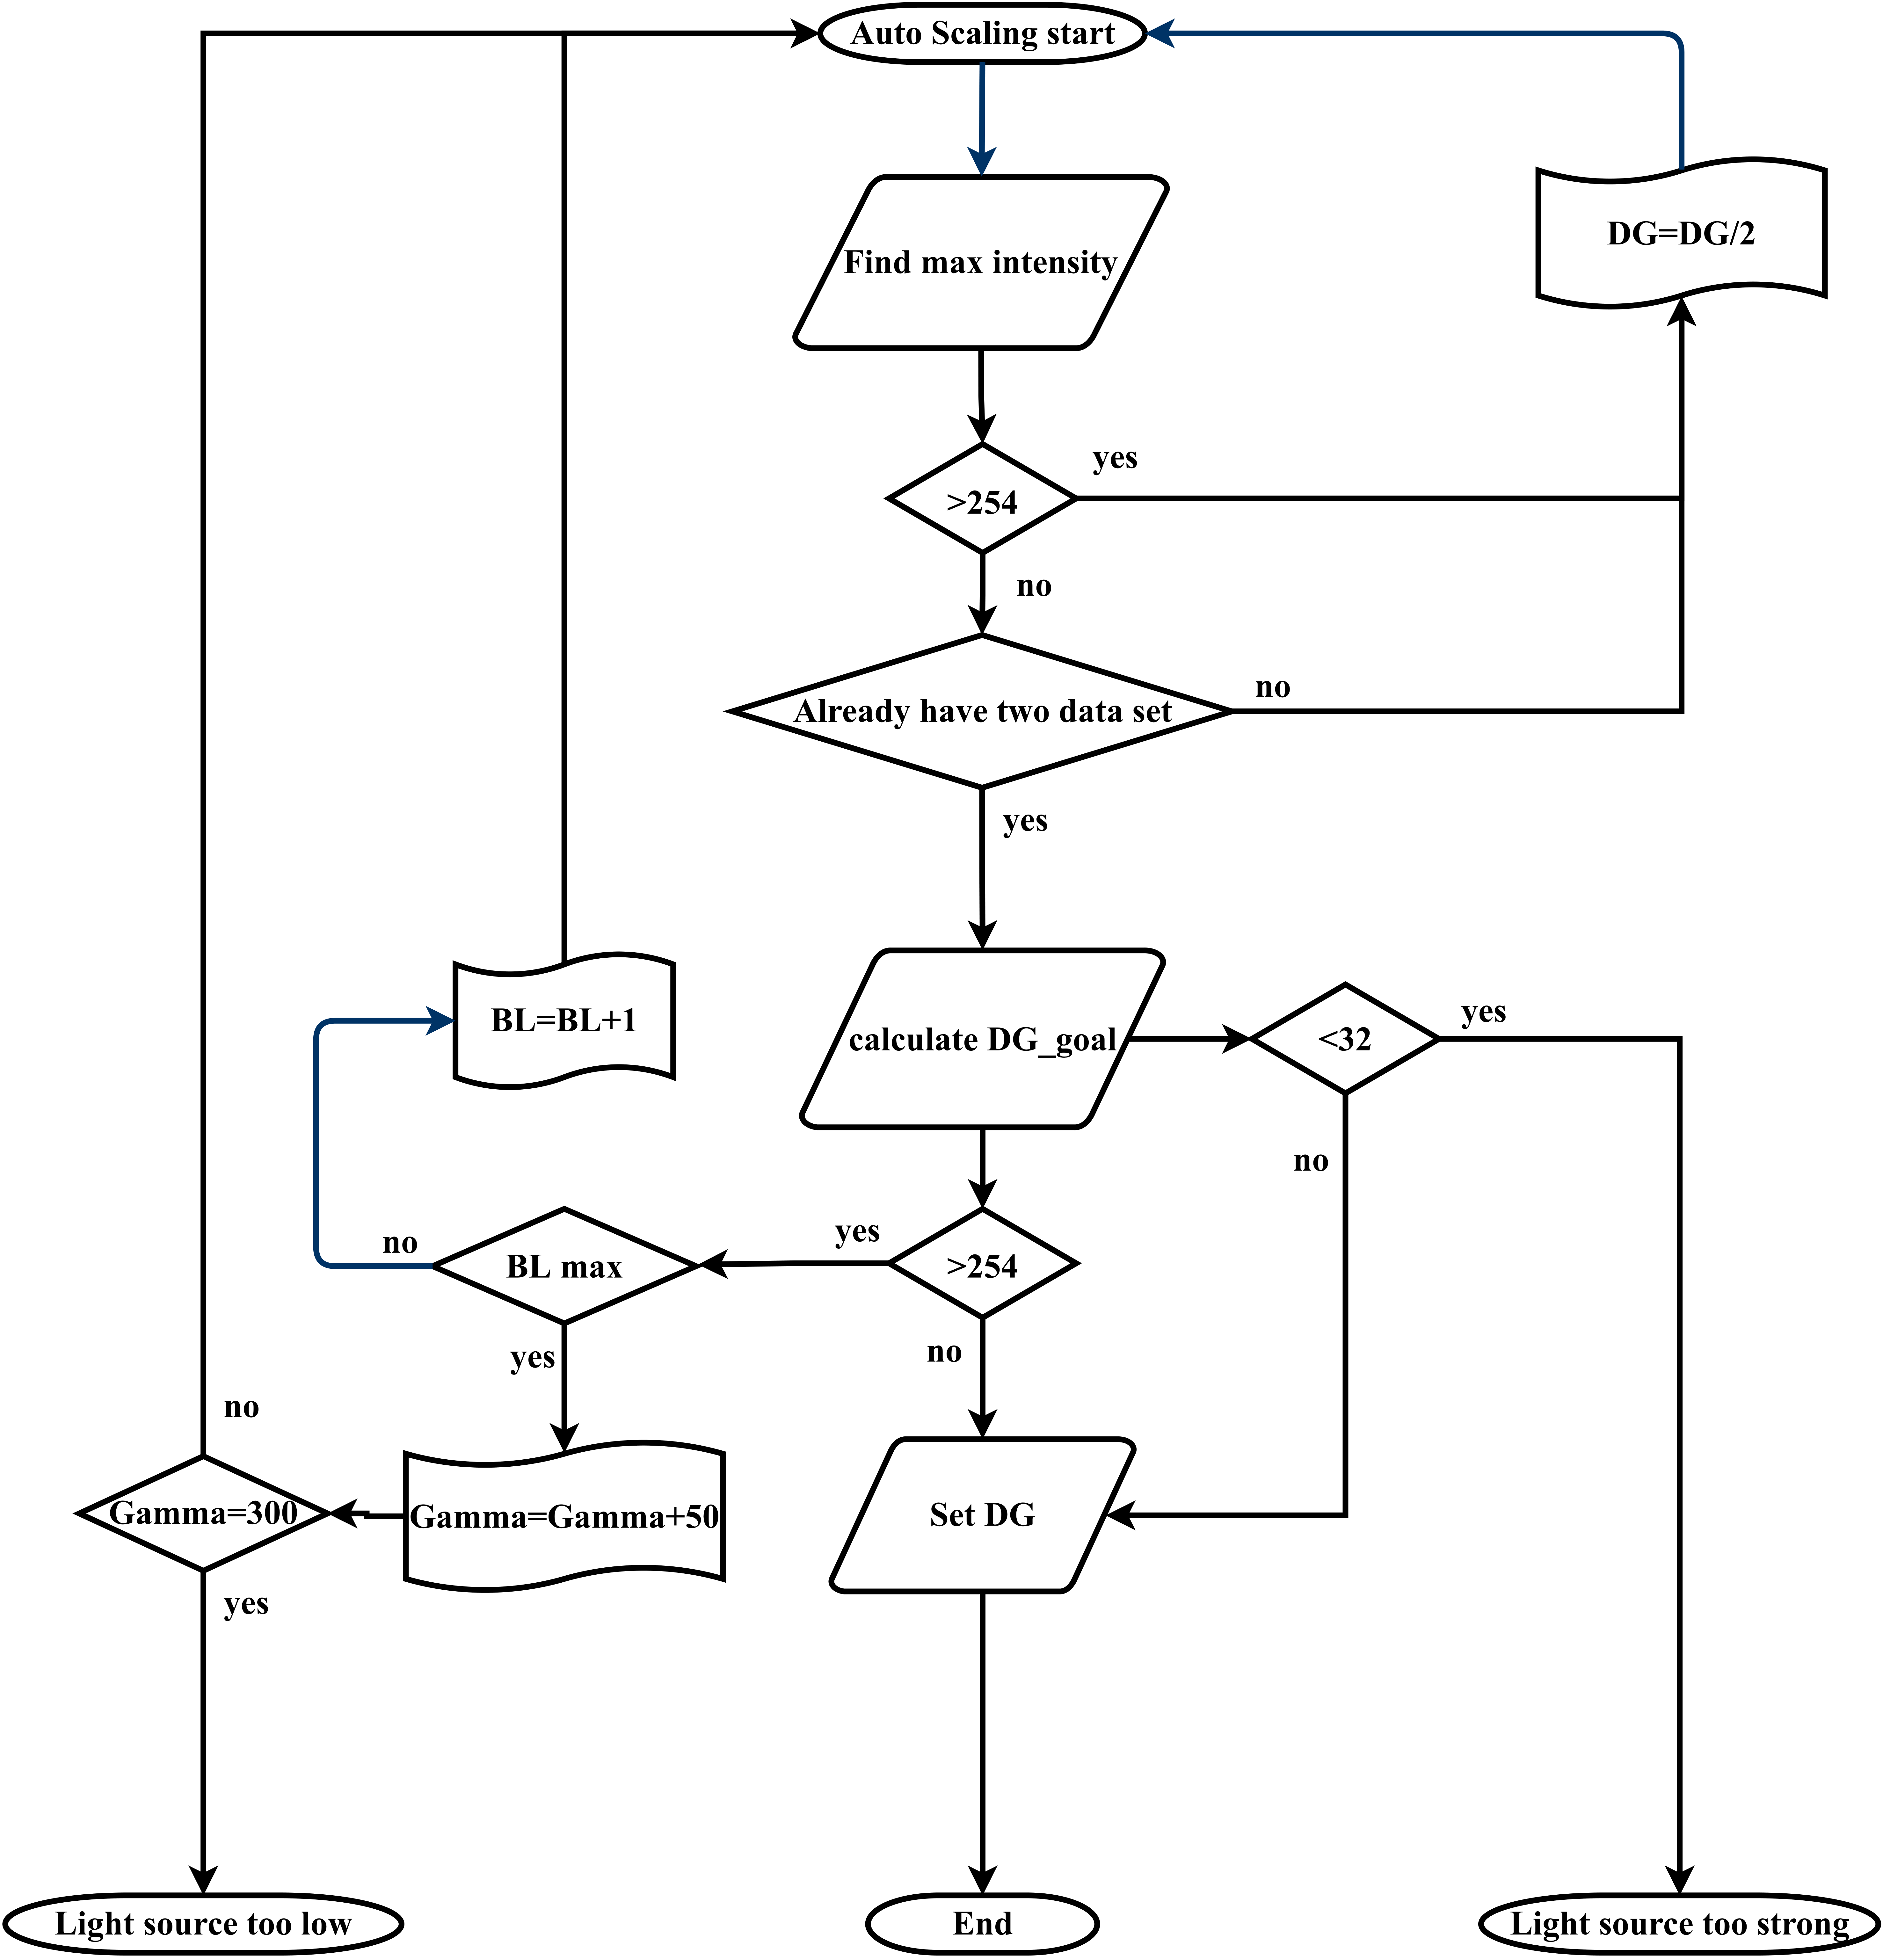
\includegraphics[width=\textwidth]{figures/Auto Scaling流程.png} %插入图片,[]中设置图片大小,{}中是图片文件名
	\caption{Auto Scaling流程圖} %最终文档中希望显示的图片标题
	\label{Auto Scaling流程圖} %用于文内引用的标签
\end{figure}

\newpage
\section{波峰位置偵測}
Auto Scaling後的光譜波形十分適合分析,由於不存在任何過曝點,故擬合後找出的峰值較為精確。本文欲結合使用雷射光與汞氬燈的波峰位置的像素與其標準參考波長做為波長校正之擬合點,因此需個別找出兩種光源的參考波峰,並經由勞倫茲擬和找出精確波峰位置,並存於記憶體之中,直至所有波峰位置皆被找出,便可以將所有波峰的像素位置與標準波長一起進行多項式擬合。\par
完整波峰查詢的標準流程如圖\ref{波峰位置偵測流程圖}. ,,但又因汞燈與氬燈強度差異過大,加上不同晶片於不同波段效率不同,礙於這兩點演算法上難以解決的困難,因此汞氬燈光譜進行波峰位置偵測前,將對數據進行汞燈與氬燈的分離,並在不同的影像感測器參數下,分別取出光譜後再進行波峰位置偵測,詳細流程本文於3.5.1節說明。
\begin{figure}[H] %H为当前位置,!htb为忽略美学标准,htbp为浮动图形
	\centering %图片居中
	\vspace{0.8cm}
	\setlength{\abovecaptionskip}{0.8cm}
	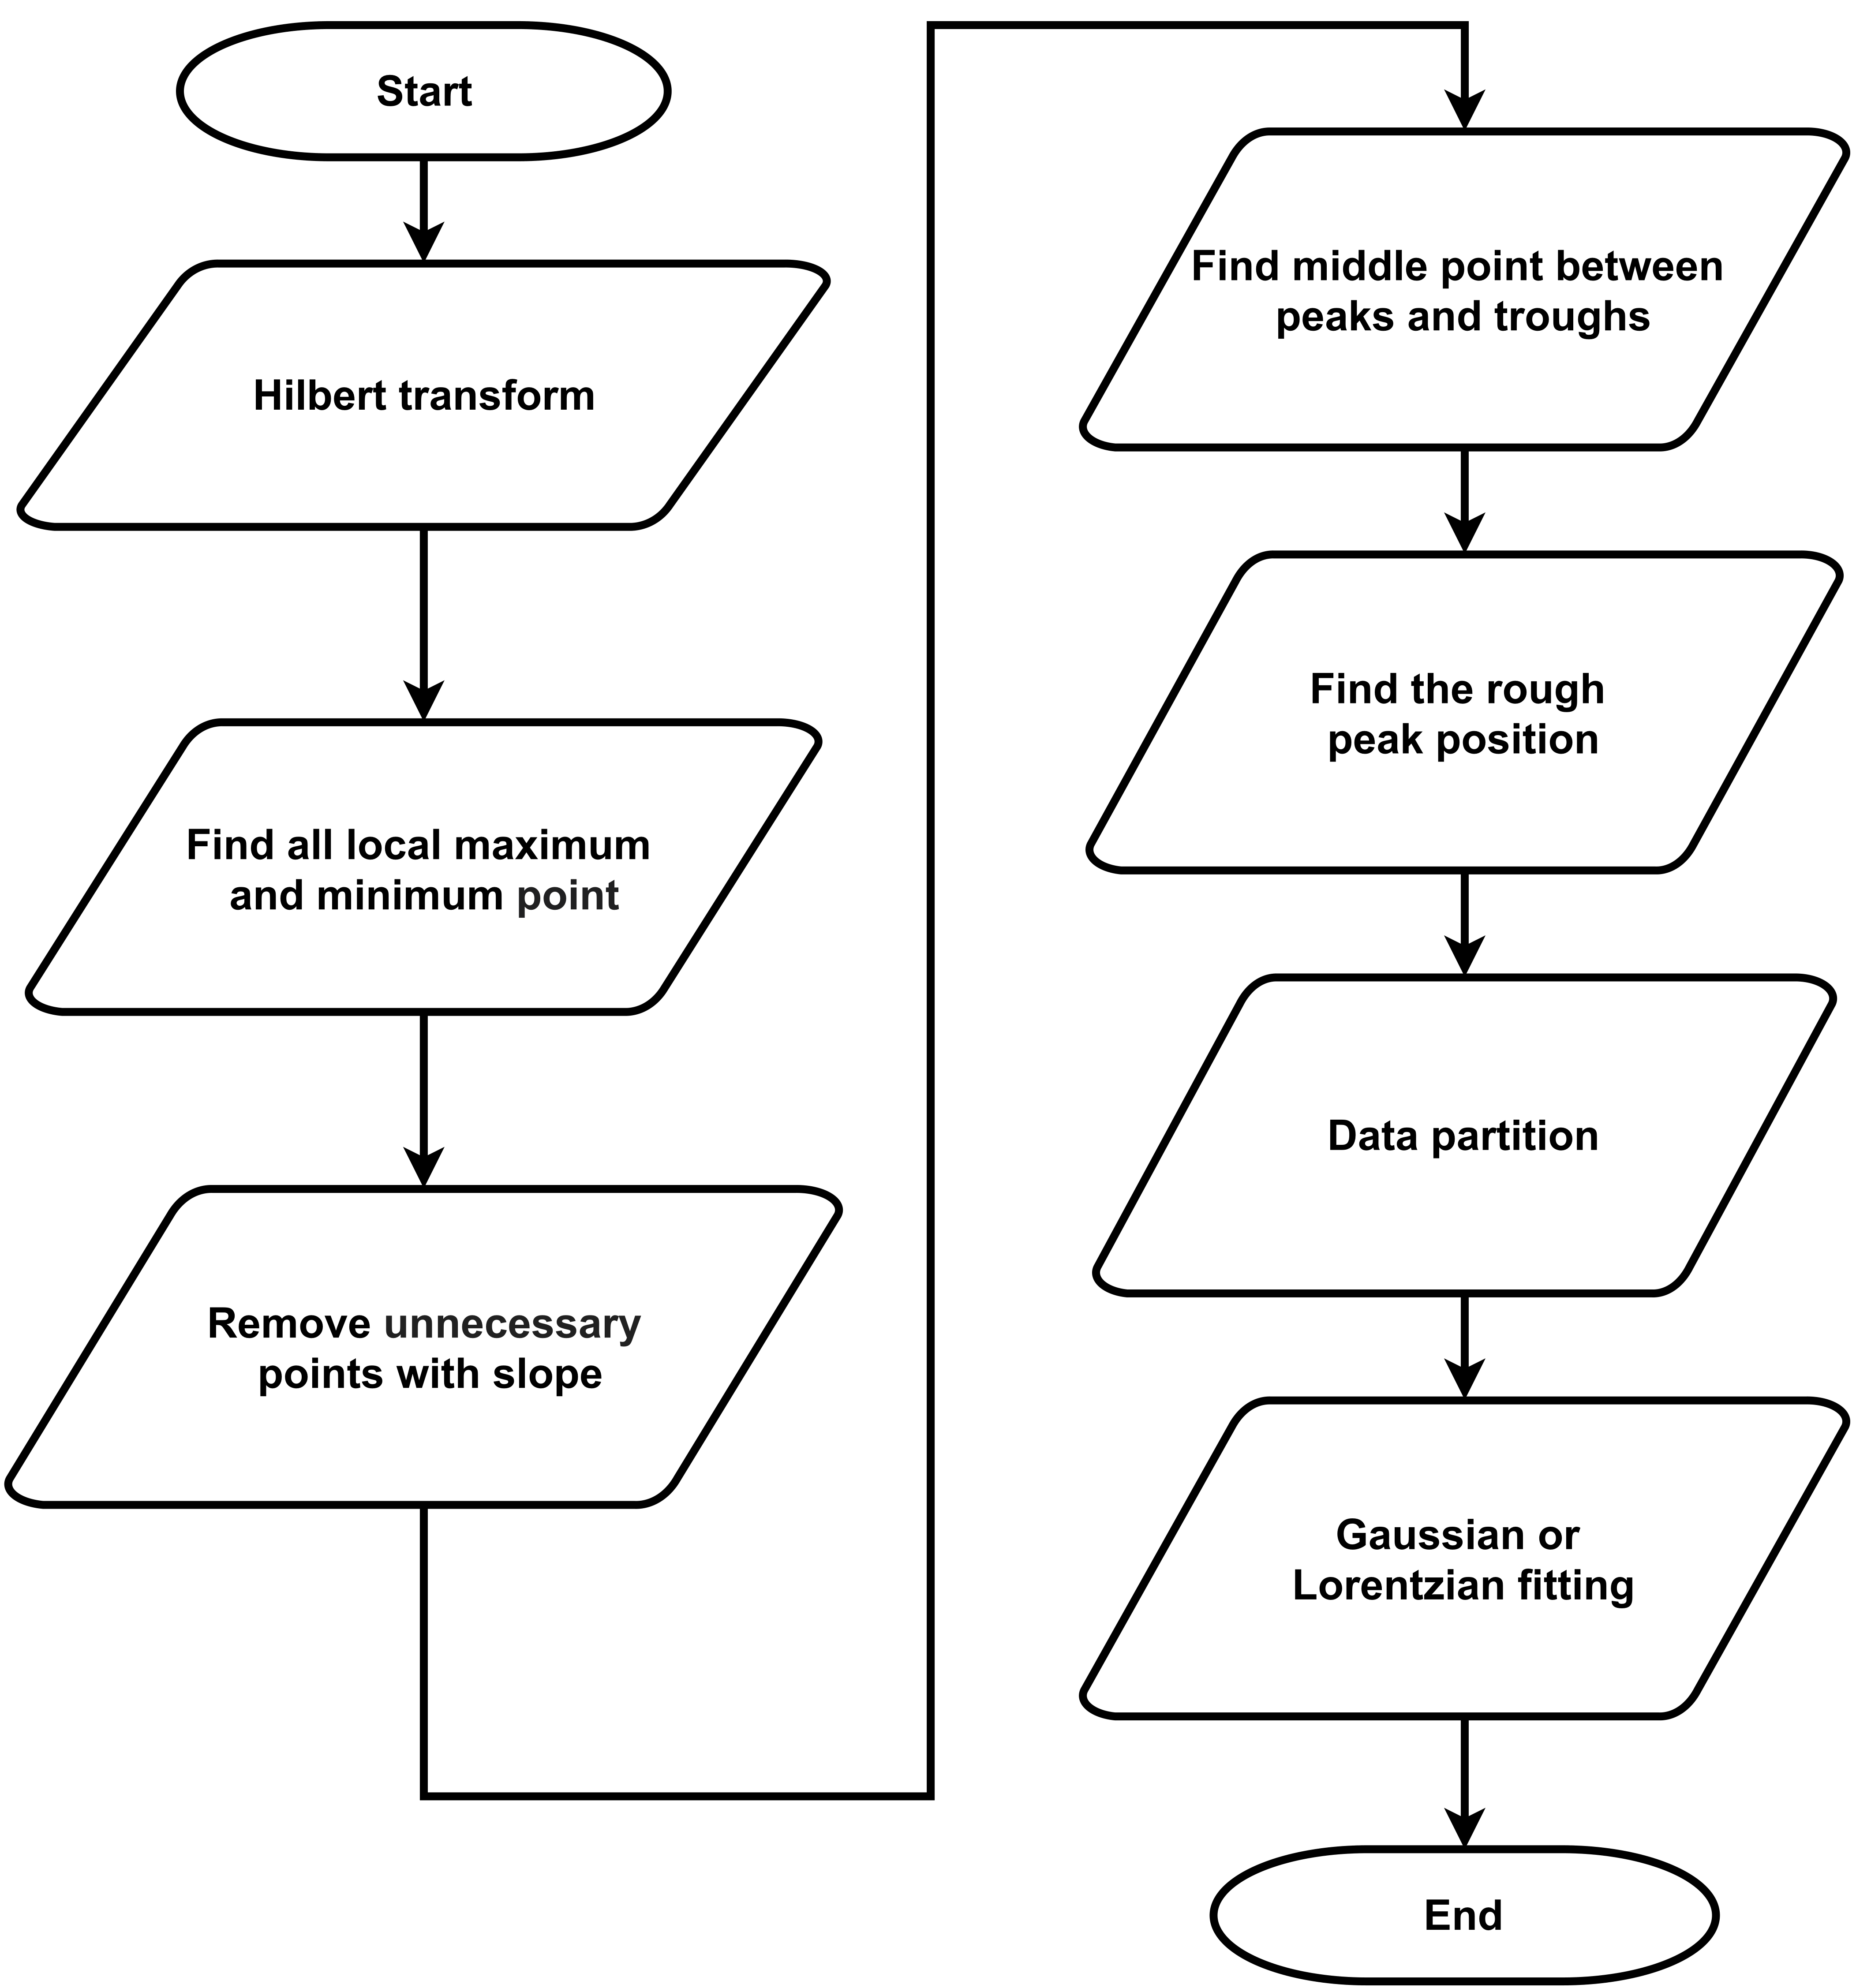
\includegraphics[width=0.7\textwidth]{figures/FINDPEAK_FLOWCHART.png} %插入图片,[]中设置图片大小,{}中是图片文件名
	\caption{波峰位置偵測流程圖} %最终文档中希望显示的图片标题
	\label{波峰位置偵測流程圖} %用于文内引用的标签
\end{figure}

\subsection{汞氬燈波峰位置偵測}
當一汞氬燈的ROI影像經過Auto Scaling後的光譜如圖\ref{Auto Scaling後汞氬燈光譜圖}. 所示,汞氬燈中的汞燈與氬燈為同時激發產生之光束,因此無法將兩數據分離,而汞燈強度與氬燈強度明顯相差極大,造成演算法難以在不同效率的晶片下穩定找到每一個波峰,所以汞燈與氬燈並非所有波峰皆適合用於波長校正,必需挑選符合要求並穩定的波峰。
\par 
適合做為波長校正波峰的條件為特徵明顯且峰與峰之間不宜距離過近,距離過近的峰值對於擬和的貢獻並不大,因此本文挑選適合做為波長校正參考波峰的汞燈與氬燈波峰的標準波長位置如表\ref{汞氬燈標準波峰位置表}. 所示。
\begin{figure}[H] %H为当前位置,!htb为忽略美学标准,htbp为浮动图形
	\centering %图片居中
	\vspace{0.8cm}
	\setlength{\abovecaptionskip}{0.cm}
	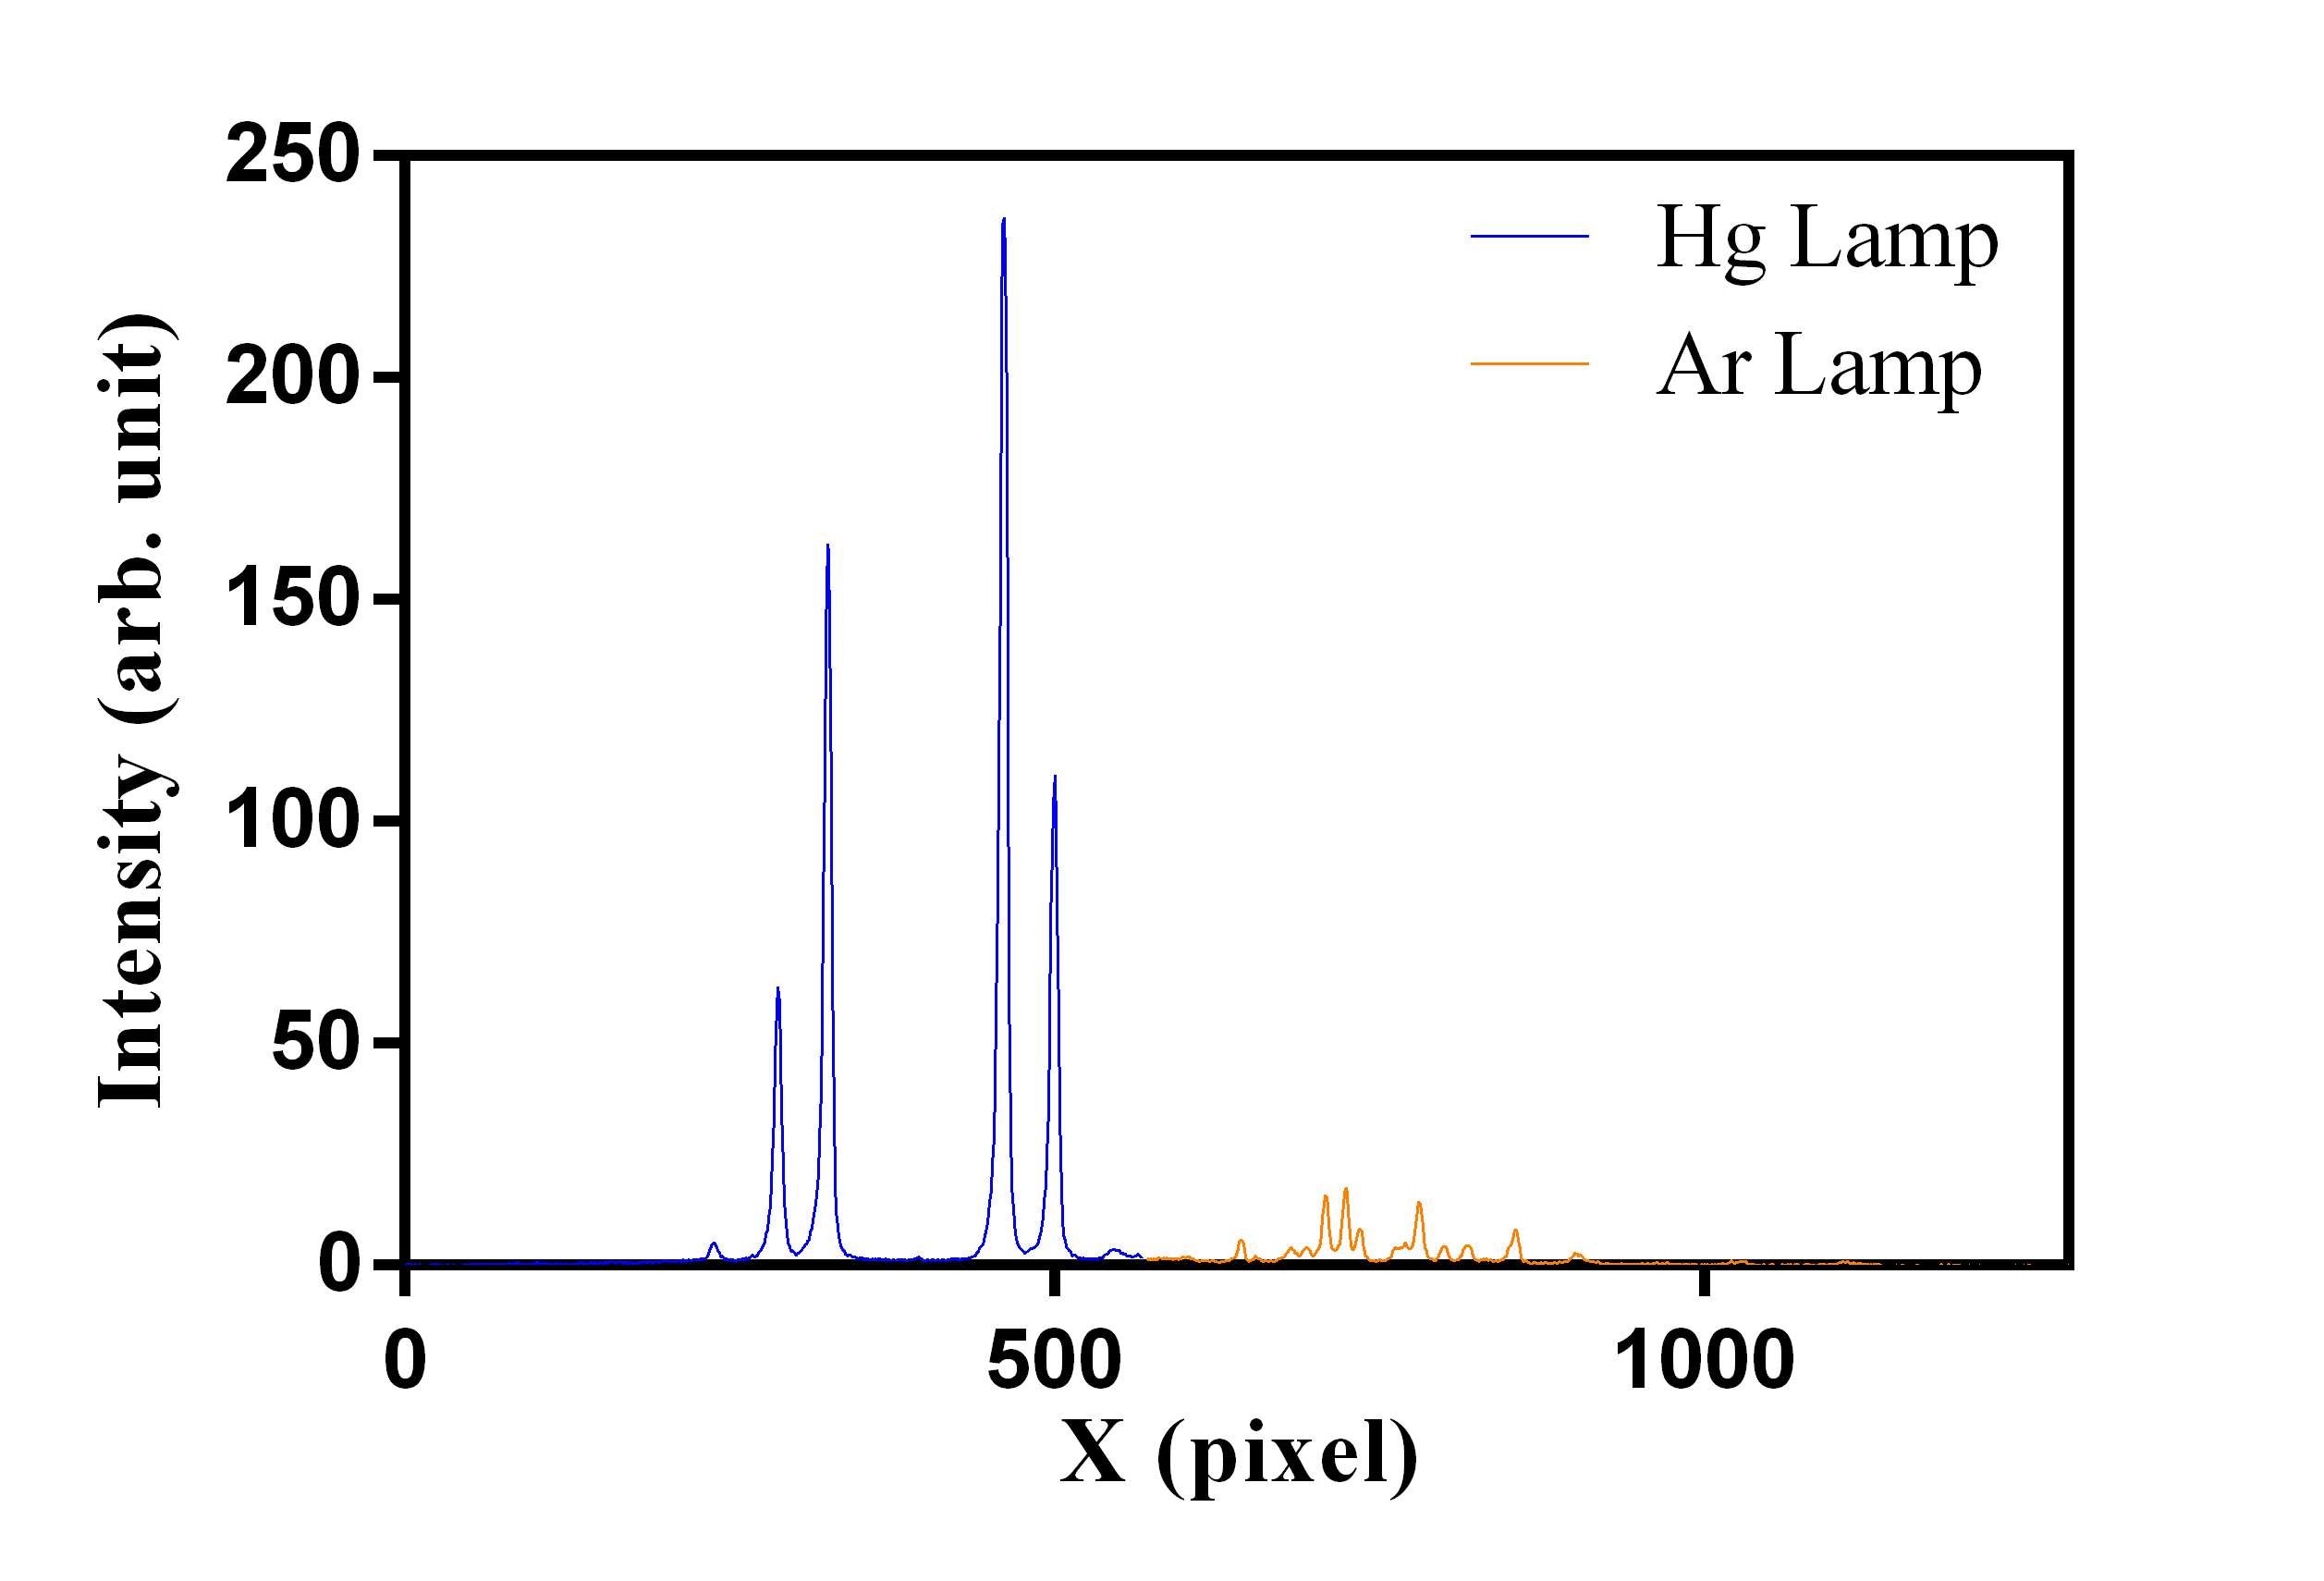
\includegraphics[width=\textwidth]{figures/HG_AR_LAMP.PNG} %插入图片,[]中设置图片大小,{}中是图片文件名
	\caption{Auto Scaling後汞氬燈光譜圖} %最终文档中希望显示的图片标题
	\label{Auto Scaling後汞氬燈光譜圖} %用于文内引用的标签
\end{figure}
\newpage
\begin{center}
\vspace{0.8cm}
\captionof{table}{汞氬燈標準波峰位置表}\label{汞氬燈標準波峰位置表}
\begin{tabularx}{\textwidth}{m{0.33\textwidth}<{\centering} m{0.25\textwidth}<{\centering} m{0.33\textwidth}<{\centering}}
	\hline\hline
          & 汞燈 & 氬燈 \\
	\hline
	\multirow{4}{*}{標準波峰位置(nm) }
	      & 404.65 & 763.51 \\
	      & 435.83 & 811.53 \\
	      & 546.07 & -- \\
	      & 578.01 & -- \\
	\hline\hline
\end{tabularx}
\vspace{10pt}
\end{center}
\par
表\ref{汞氬燈標準波峰位置表}. 中的六個波峰,橫跨短波長至長波長波段,對於每個波段皆有擬合貢獻,因此相當適合做為波長校正的擬和點,且強度較其餘波峰強的許多,利於波峰偵測,故此六個波峰為汞氬燈波峰偵測的目標波峰,而這些波峰位置在圖\ref{汞氬燈目標波峰位置圖}. 標示於波長空間中。
\begin{figure}[H] %H为当前位置,!htb为忽略美学标准,htbp为浮动图形
	\centering %图片居中
	\vspace{0.8cm} 
	\setlength{\abovecaptionskip}{0.cm}
	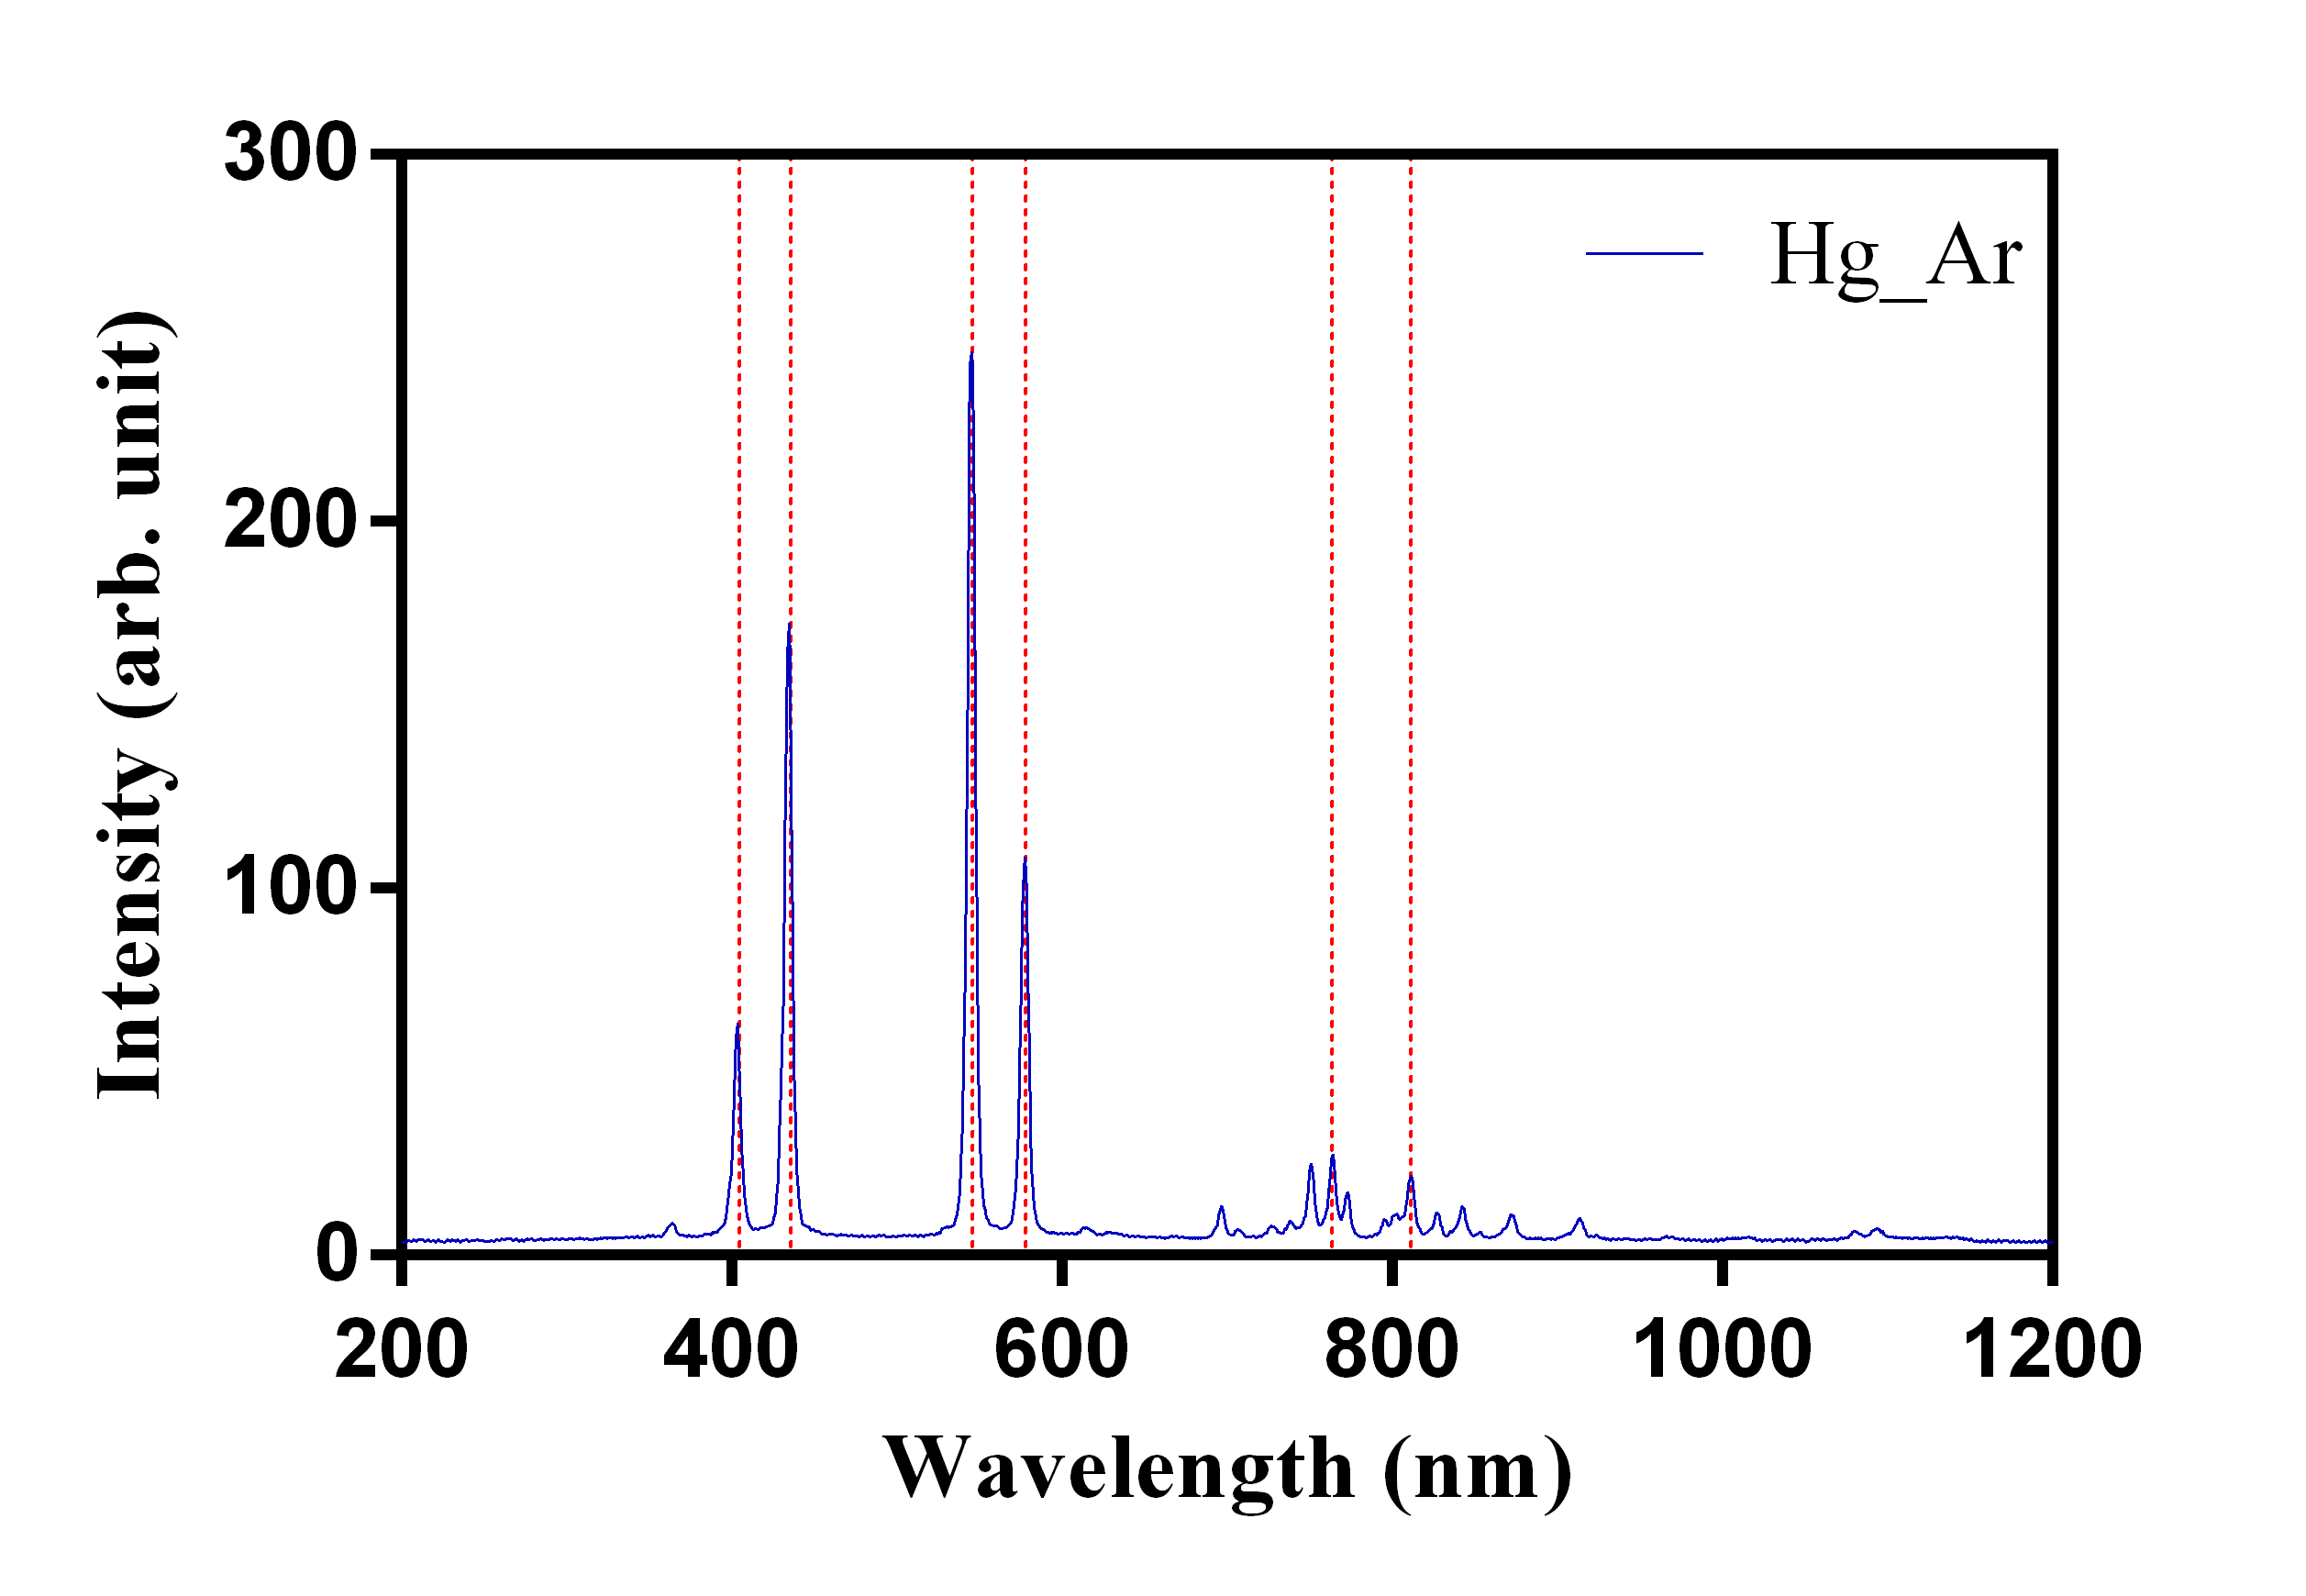
\includegraphics[width=\textwidth]{figures/HgAr_Wavelength.png} %插入图片,[]中设置图片大小,{}中是图片文件名
	\caption{汞氬燈目標波峰位置圖} %最终文档中希望显示的图片标题
	\label{汞氬燈目標波峰位置圖} %用于文内引用的标签
\end{figure}
\newpage

由於目標波峰涵蓋汞燈波峰與氬燈波峰,又因氬燈與汞燈強度落差極為巨大,造成波峰偵測時的強度閥值與斜率閥值難以界定,因不同晶片效能不同,光譜強度難以重現,若以原始數據及固定閥值界定是否為有效波峰,將會出現氬燈在效率較低之晶片時波峰無法被完全偵測,反之則在效率高的晶片時發生雜訊被判定為波峰。\par
光譜雖在像素空間會因影像感測器的因素而有平移,強度也會有所不同,造成每次量測時波峰落在不同的位置與不同的強度,但因任何物質的光譜波長位置與光譜趨勢是唯一且不變的,因此所有波峰的距離是固定的,所以不同空間中的光譜波型是不會改變的,波峰的距離也是固定的,本文利用此一光譜特性,透過數據中的最大值像素位置與像素距離界定出汞燈與氬燈的數據分界點,如圖\ref{汞氬燈數據分區交界點}. 所示。
\begin{figure}[H] %H为当前位置,!htb为忽略美学标准,htbp为浮动图形
	\centering %图片居中
	\vspace{0.8cm}
	\setlength{\abovecaptionskip}{0.cm}
	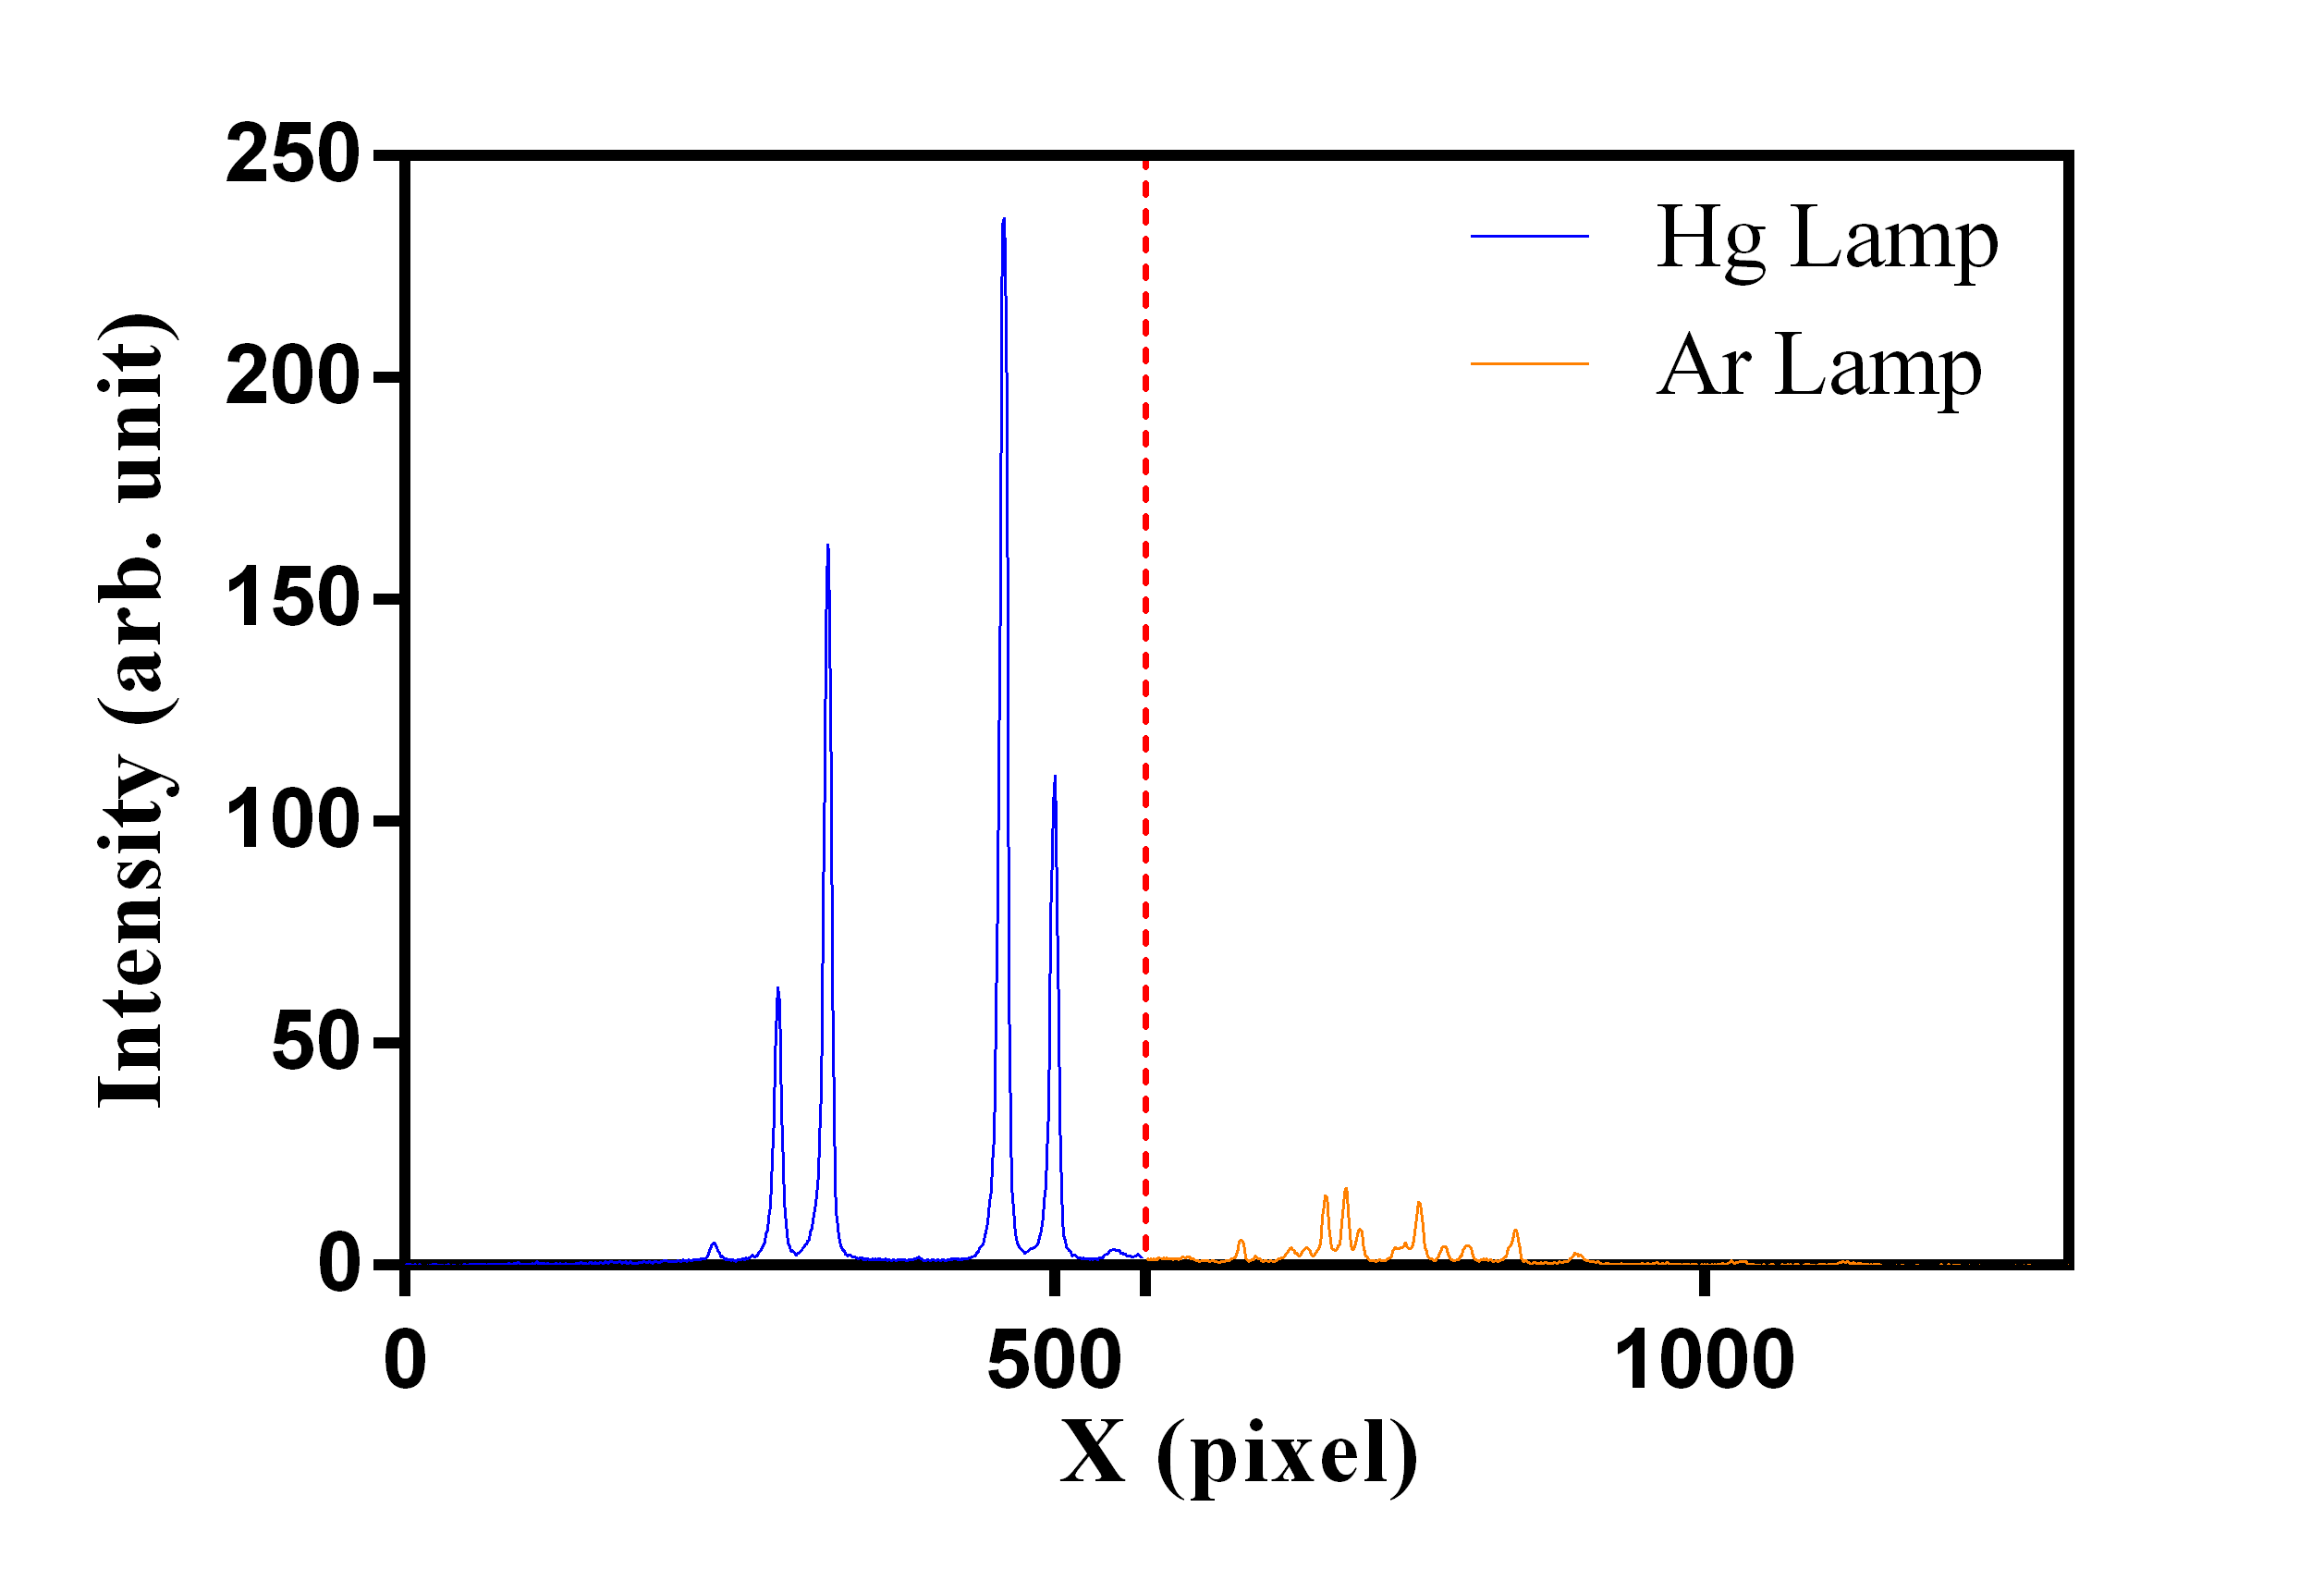
\includegraphics[width=\textwidth]{figures/JunctionPoint.png} %插入图片,[]中设置图片大小,{}中是图片文件名
	\caption{汞氬燈數據分區交界點} %最终文档中希望显示的图片标题
	\label{汞氬燈數據分區交界點} %用于文内引用的标签
\end{figure}
將汞燈氬燈數據個別區分後,由於此組原始數據已經進行過一次Auto Scaling,因此汞燈區域已完成強度調整,僅需對氬燈區域數據再進行一次Auto Scaling,使氬燈區域光譜強度達到適當值如圖\ref{氬燈數據AutoScaling後光譜波形圖}. 所示,再將兩組數據合併進行波峰偵測,即可達到平衡汞燈與氬燈間的強度落差,結合後光譜數據如圖\ref{氬燈數據AutoScaling並合併後光譜波形圖}. 所示。
\begin{figure}[H] %H为当前位置,!htb为忽略美学标准,htbp为浮动图形
	\centering %图片居中
	\vspace{0.8cm}
	\setlength{\abovecaptionskip}{0.cm}
	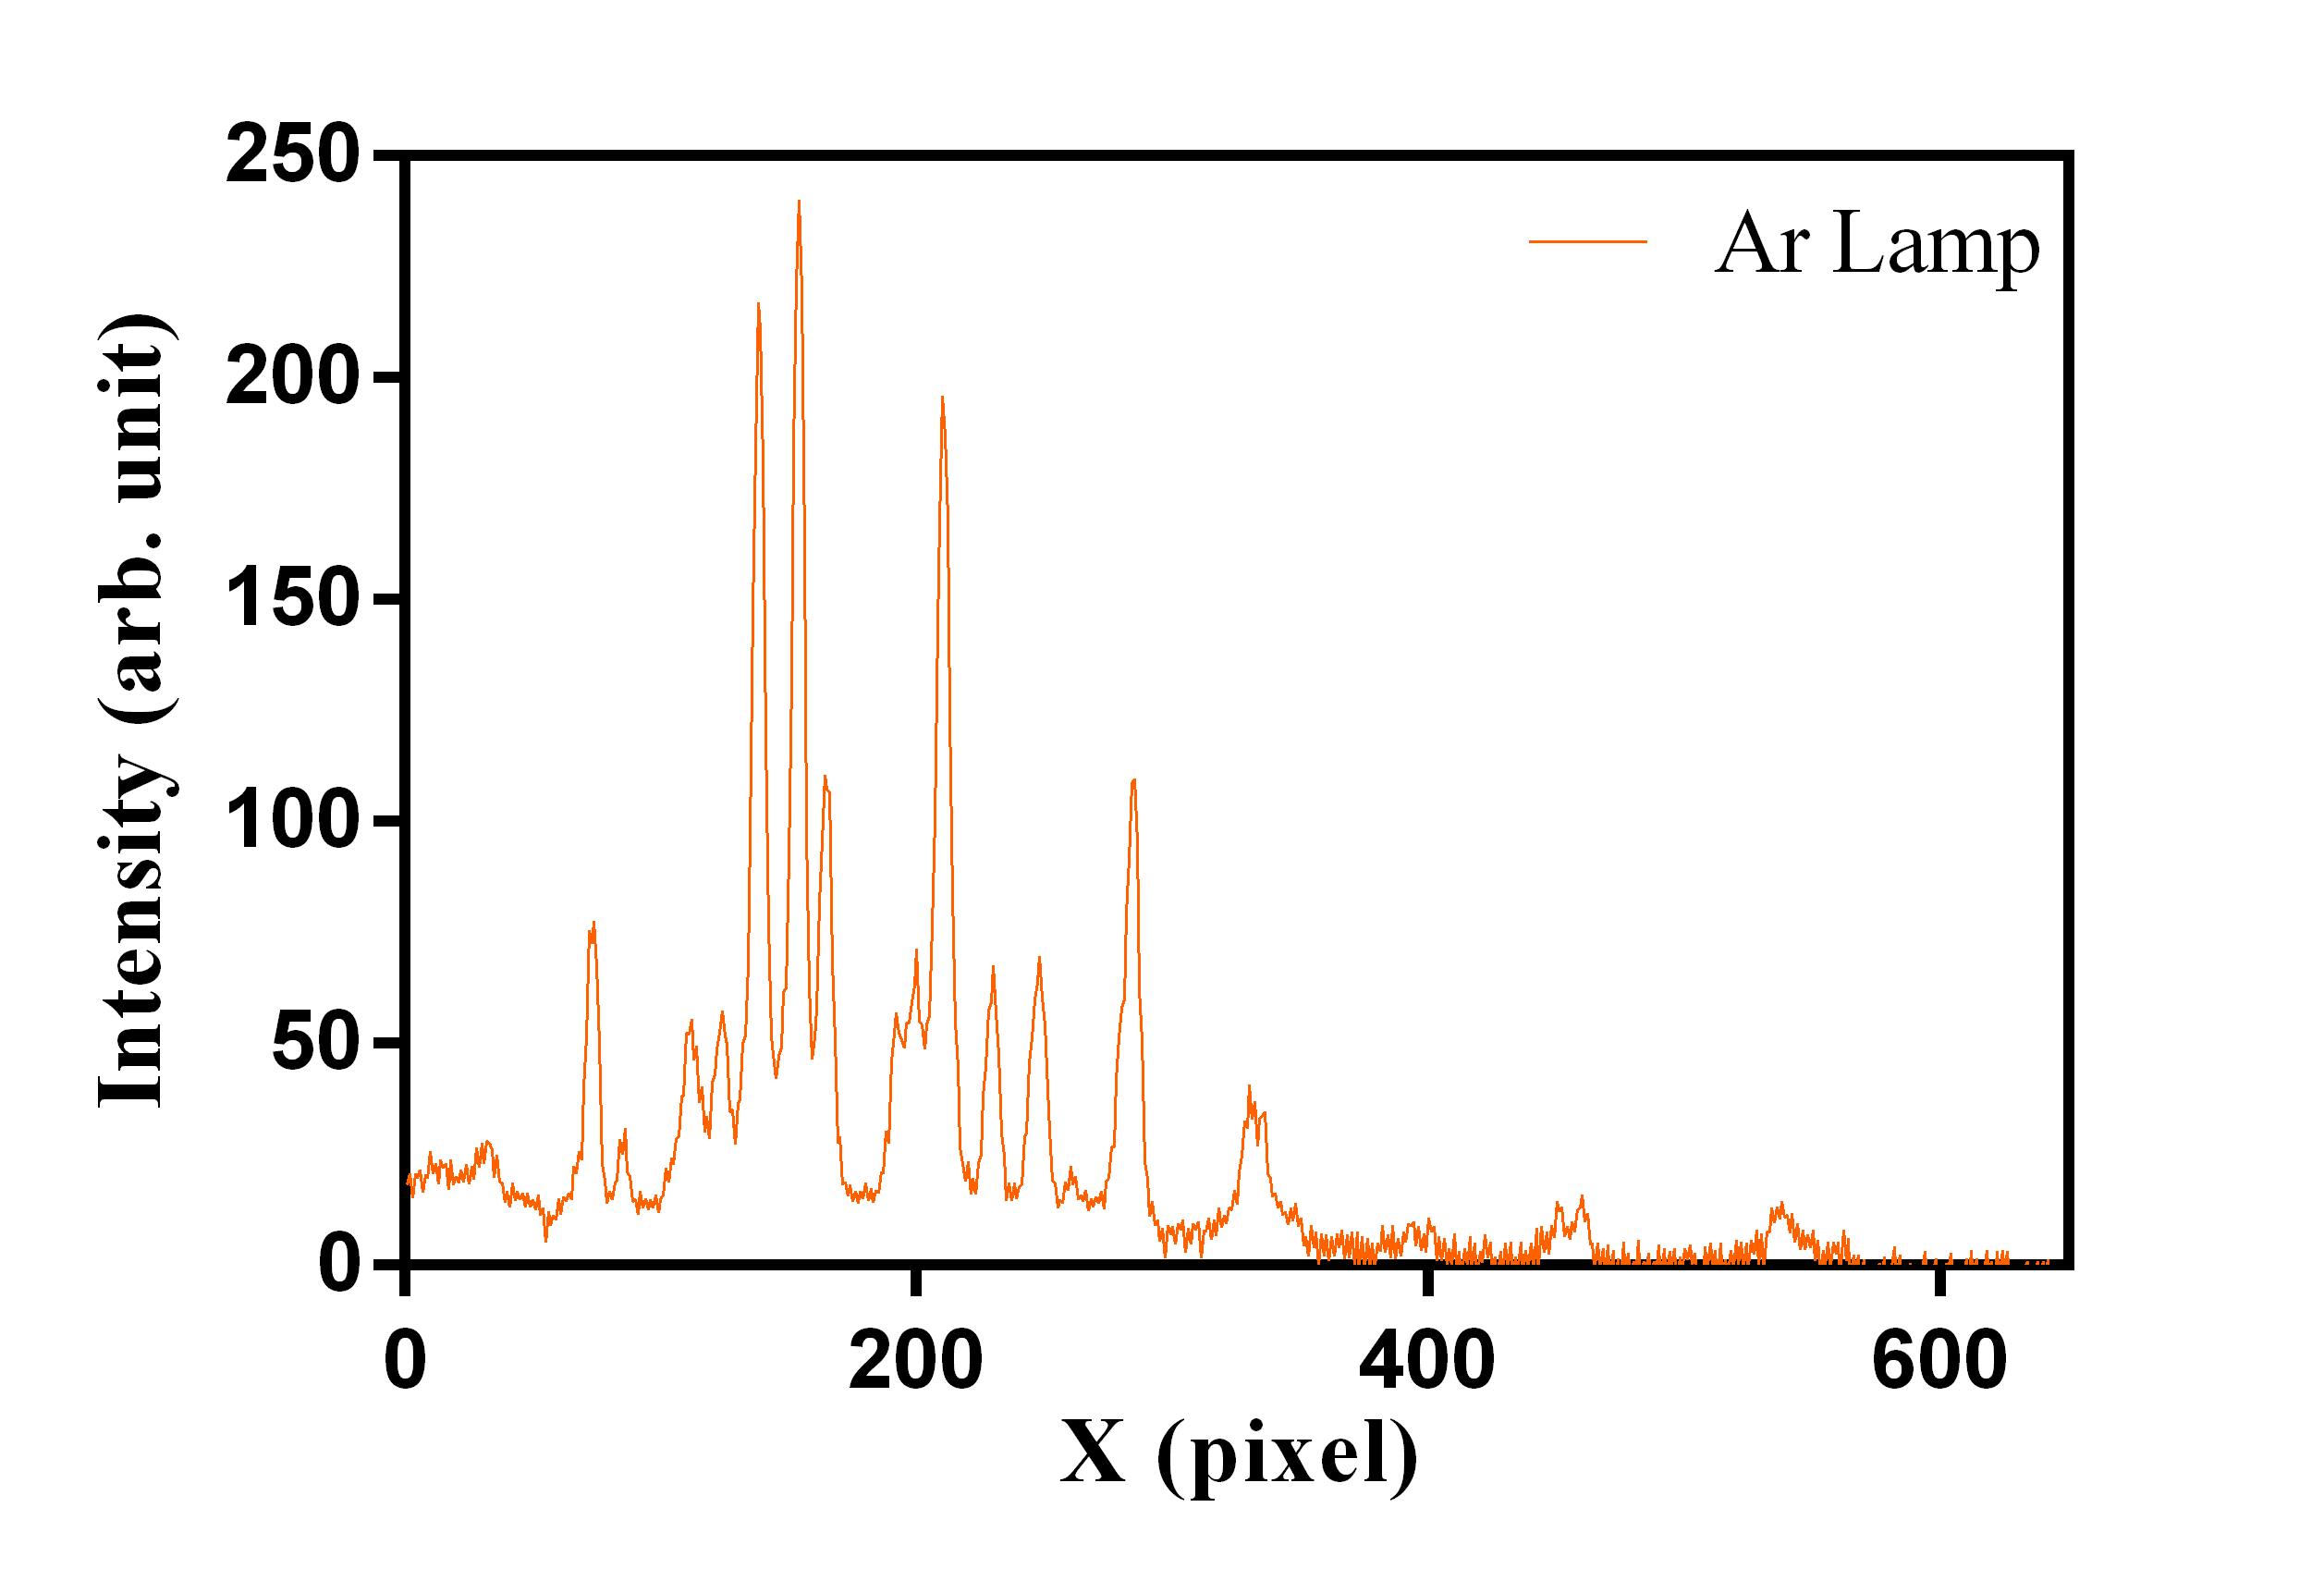
\includegraphics[width=15cm]{figures/ArLamp.png} %插入图片,[]中设置图片大小,{}中是图片文件名
	\caption{氬燈數據AutoScaling後光譜波形圖} %最终文档中希望显示的图片标题
	\label{氬燈數據AutoScaling後光譜波形圖} %用于文内引用的标签
\end{figure}

\begin{figure}[H] %H为当前位置,!htb为忽略美学标准,htbp为浮动图形
	\centering %图片居中
	\setlength{\abovecaptionskip}{0.cm}
	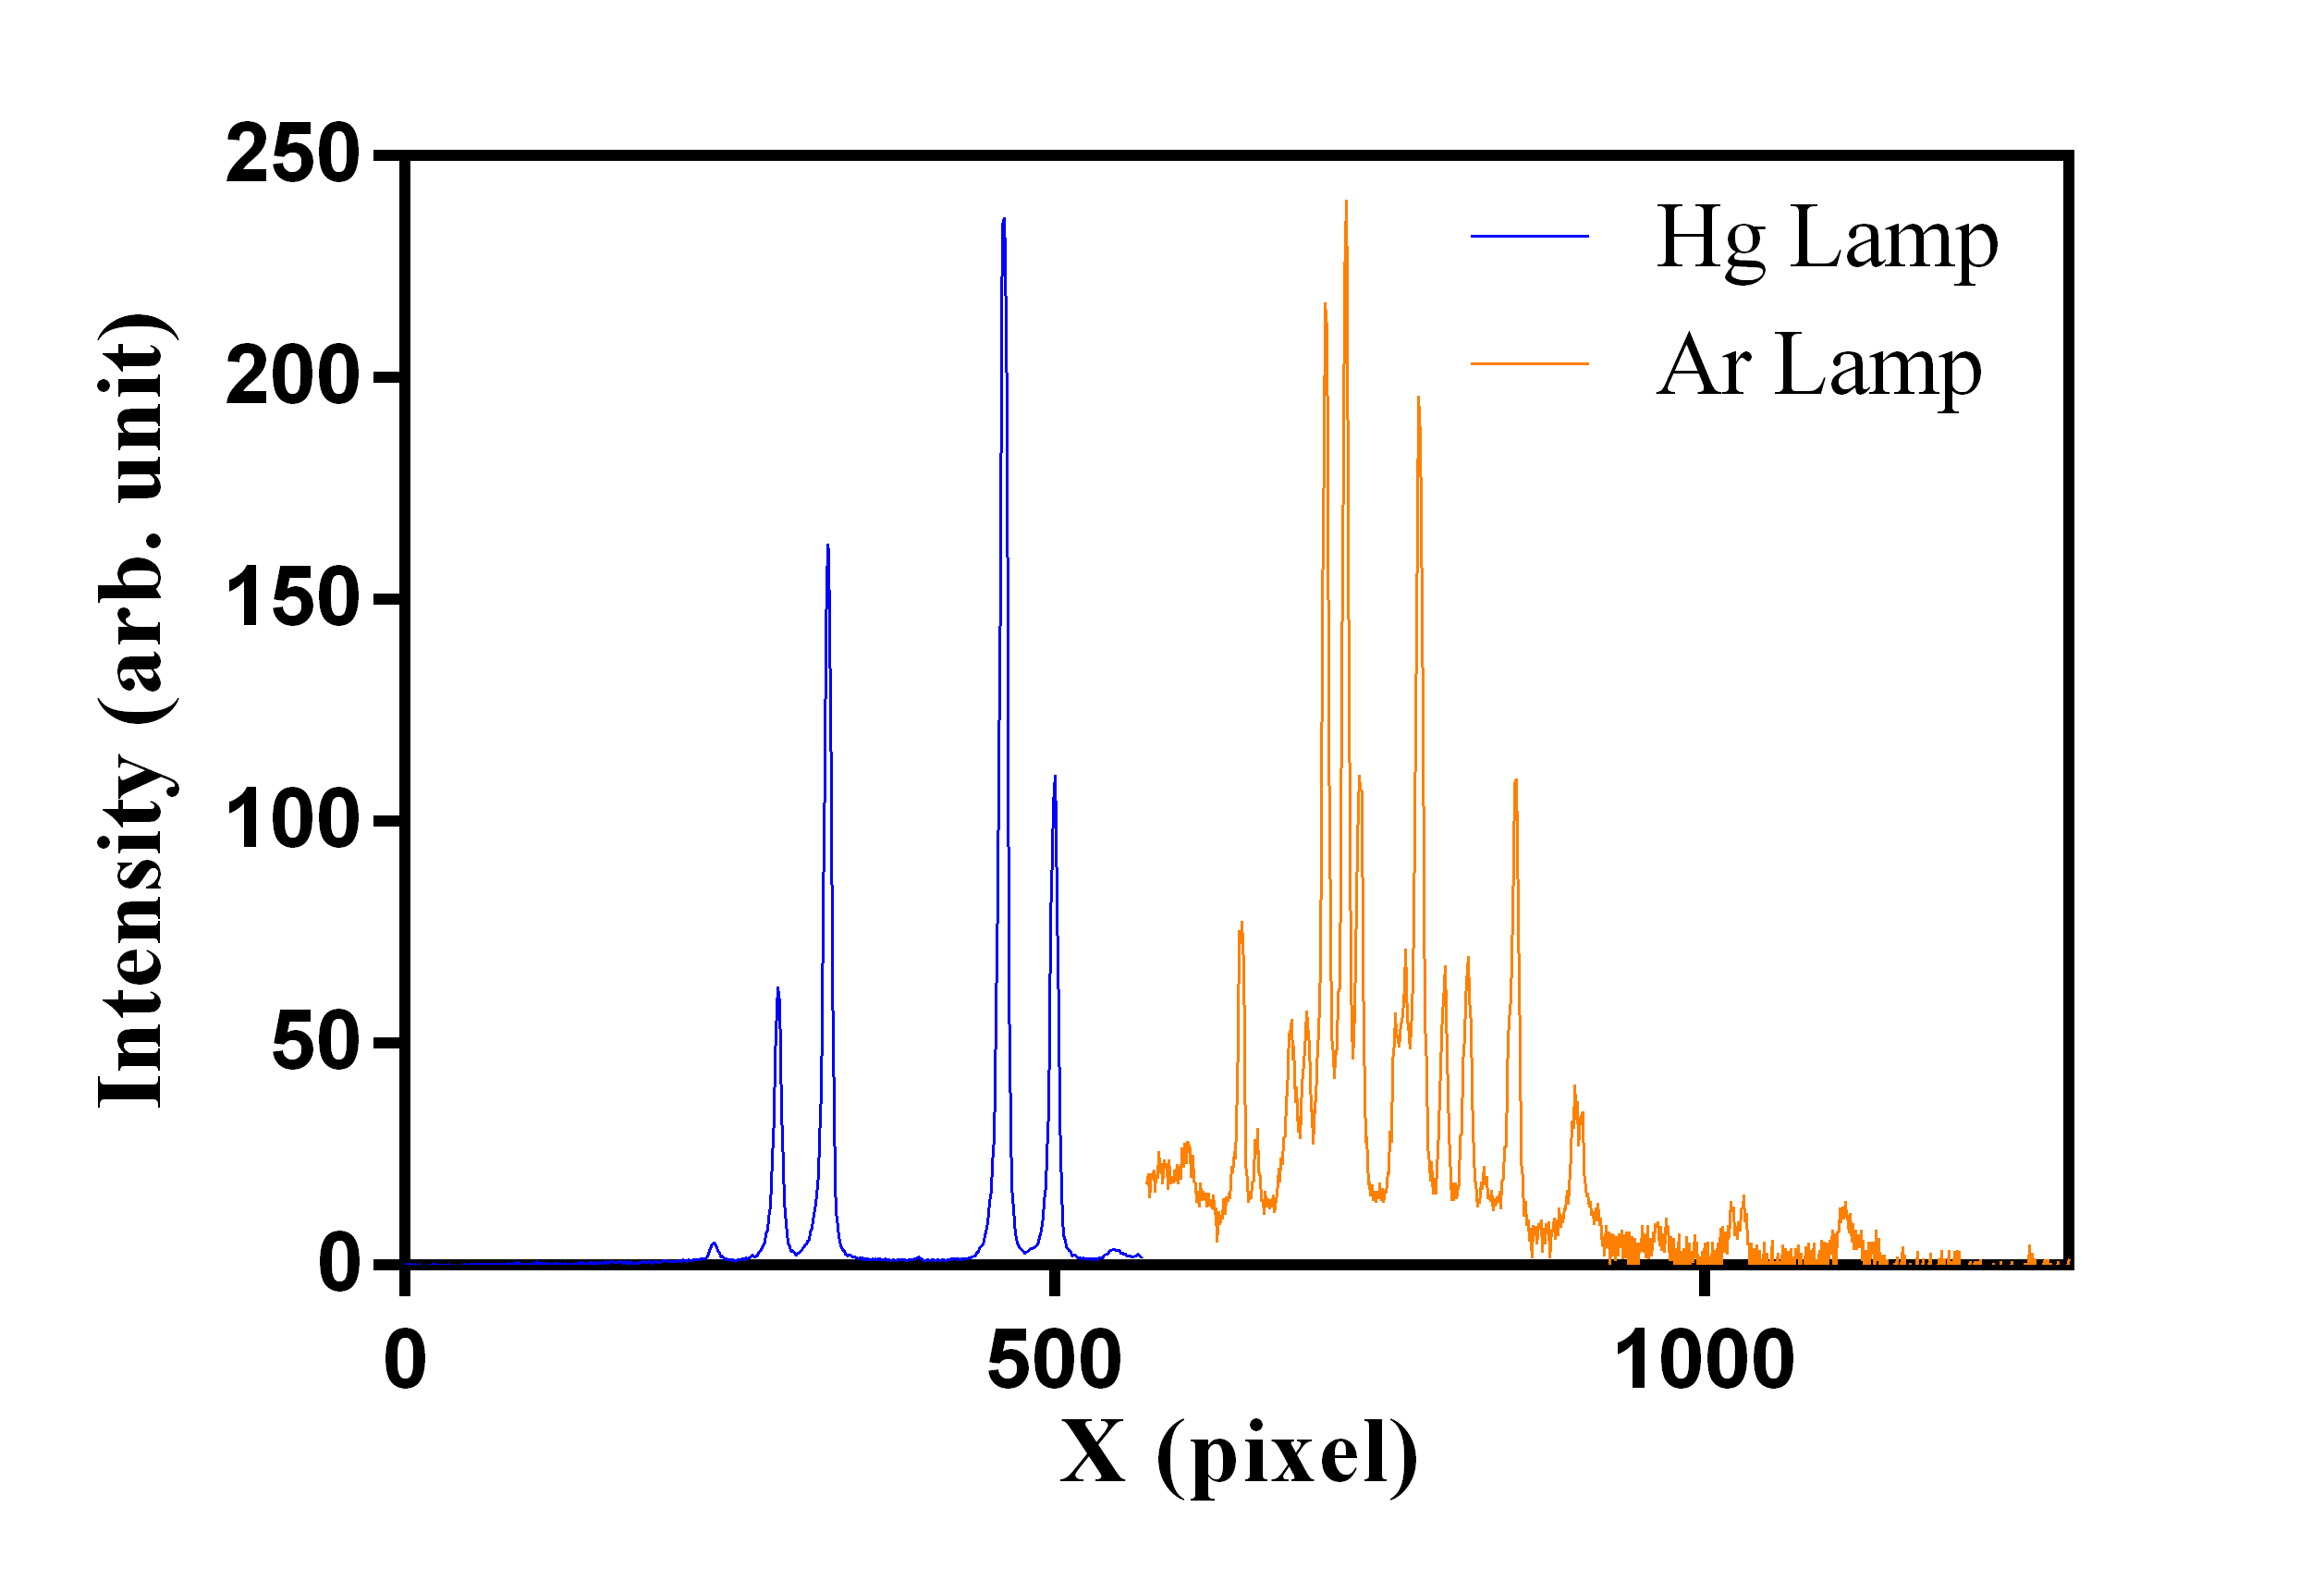
\includegraphics[width=15cm]{figures/Comebine_ArLamp.png} %插入图片,[]中设置图片大小,{}中是图片文件名
	\caption{氬燈數據AutoScaling並合併後光譜波形圖} %最终文档中希望显示的图片标题
	\label{氬燈數據AutoScaling並合併後光譜波形圖} %用于文内引用的标签
\end{figure}

波峰偵測時常以斜率\cite{slope-find-peak}作為判定方式,但因強度平衡後的汞氬燈數據也將造成氬燈區域雜訊被大幅放大,因此不宜將此數據用來以Hilbert Transform判定粗略波峰位置,故波峰偵測的第一步為將原始光譜數據進行Hilbert Transform,並找出所有轉換後的區域最大值與最小值如圖\ref{光譜經由希爾伯特轉換後的區域最大值與最小值位置}. 所示。
\begin{figure}[H] %H为当前位置,!htb为忽略美学标准,htbp为浮动图形
	\centering %图片居中
	\vspace{0.8cm}
	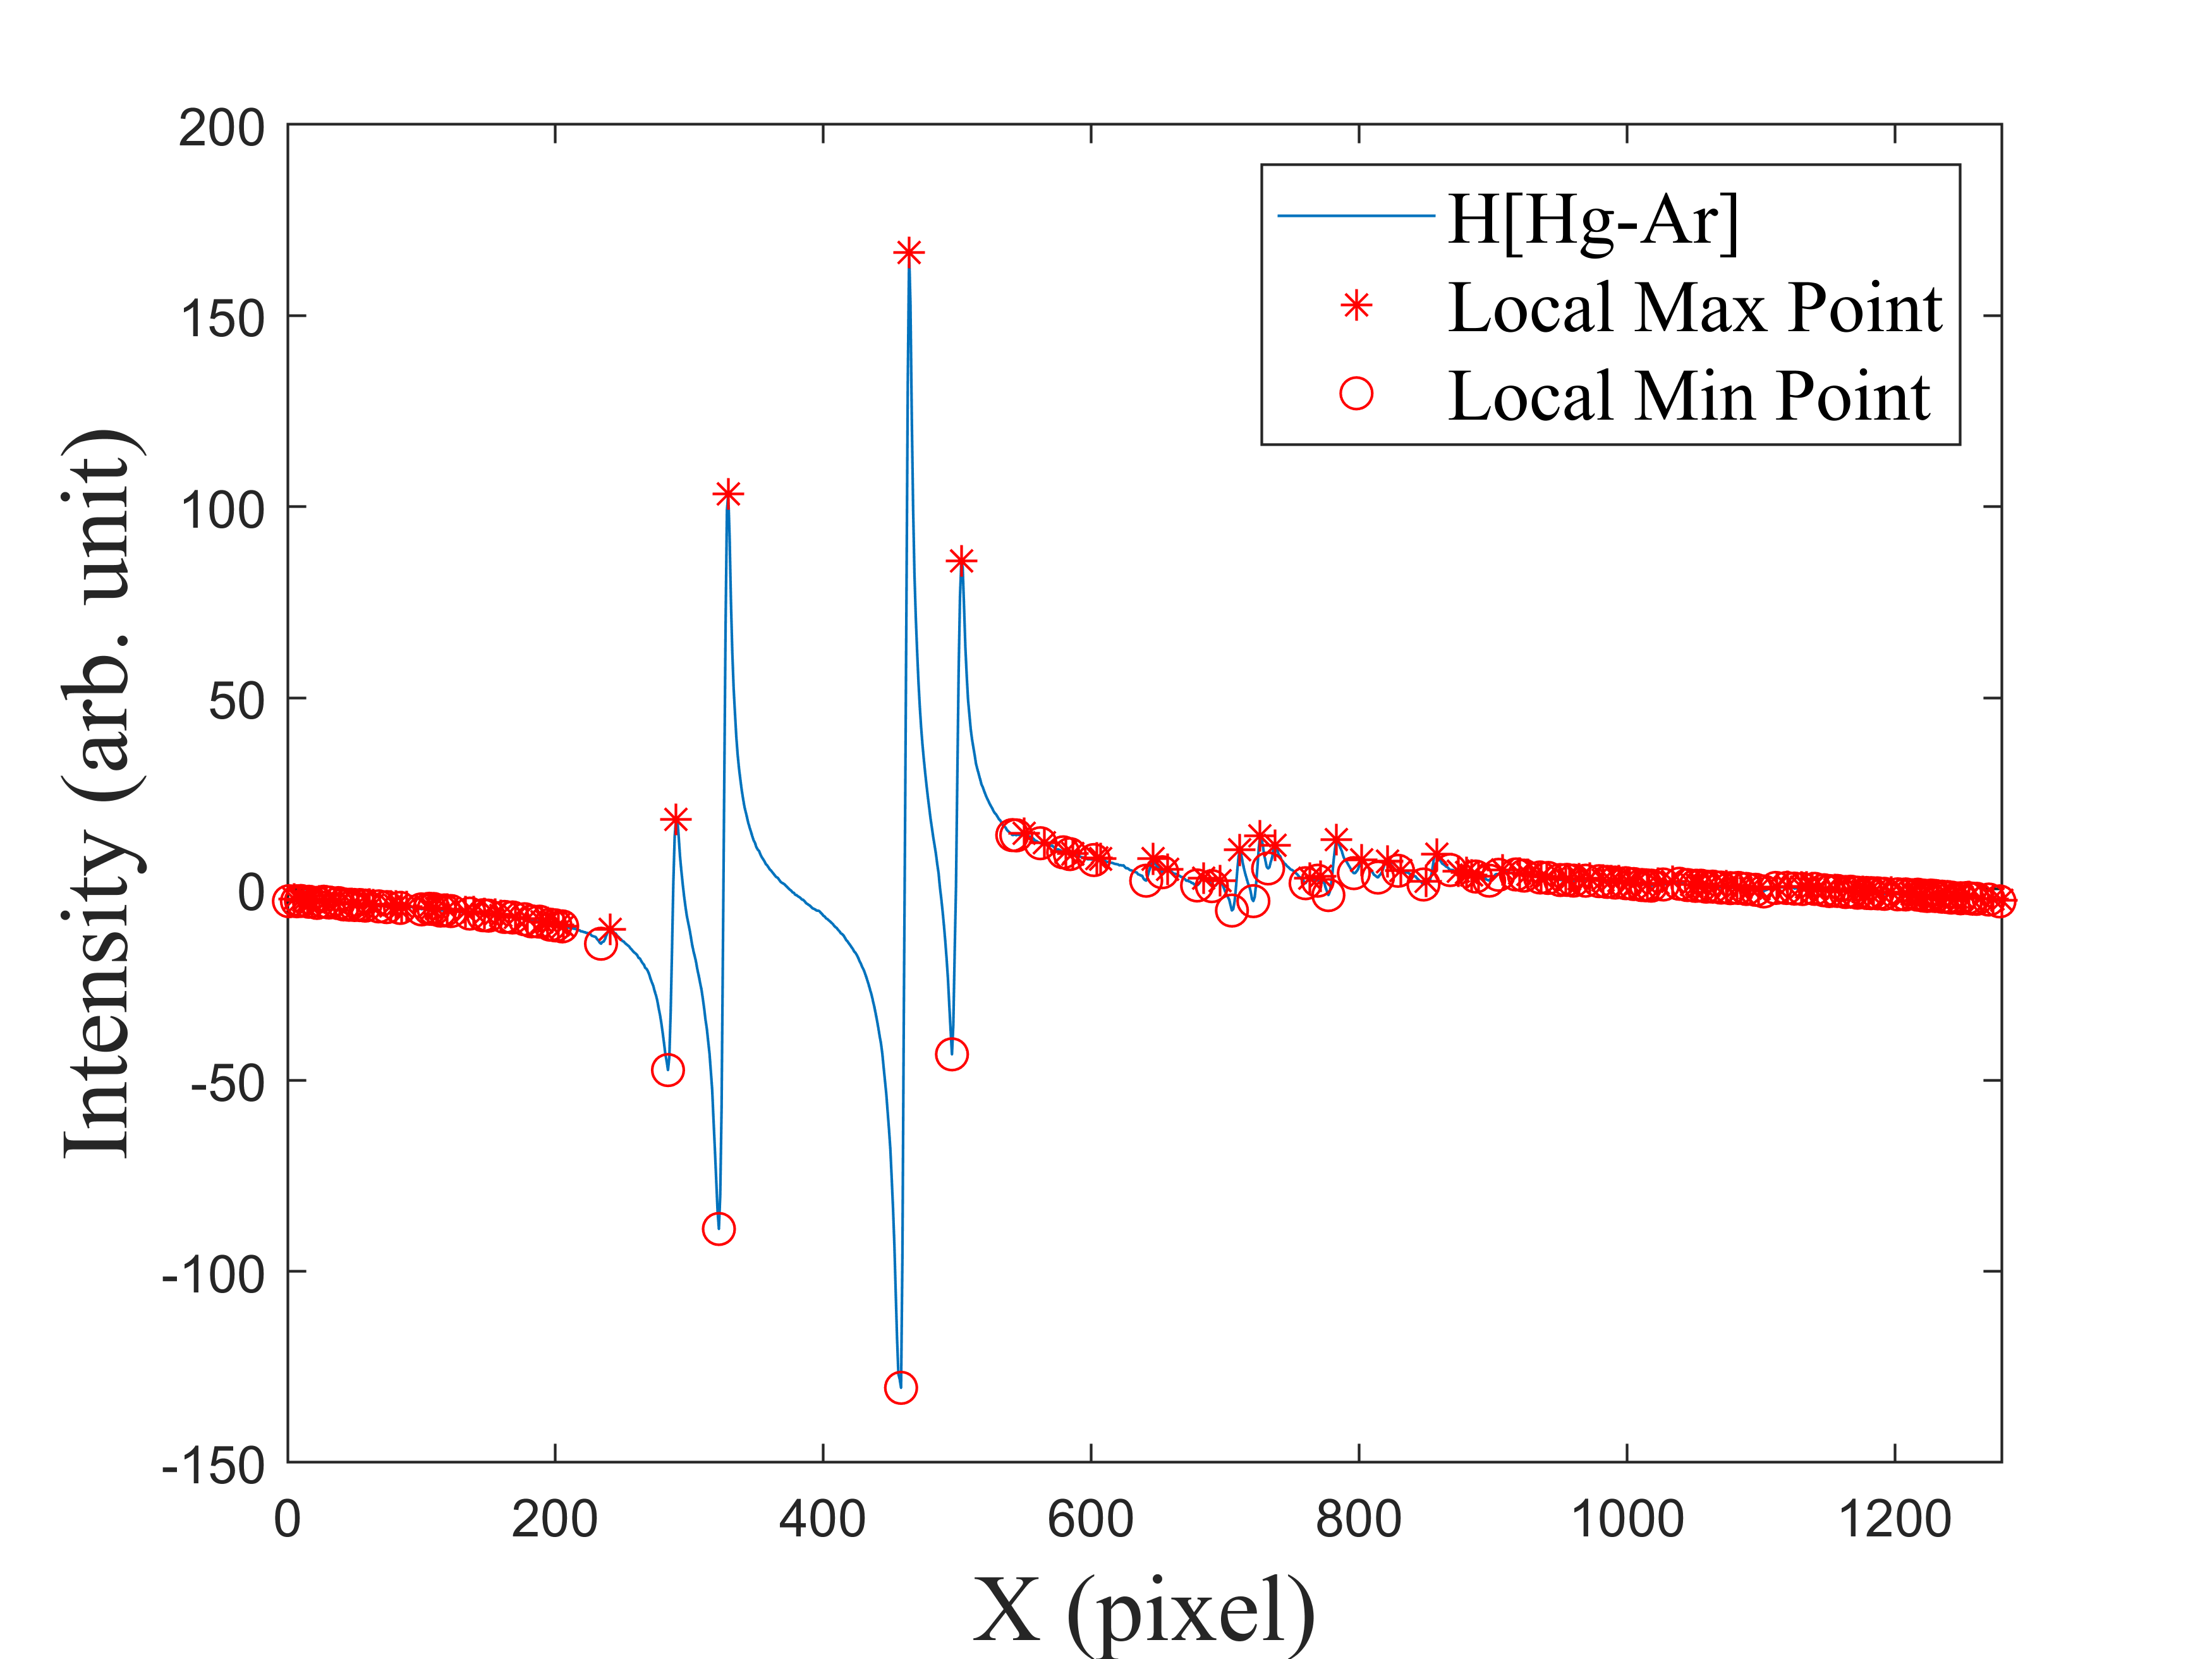
\includegraphics[width=\textwidth]{figures/Hil_HGAR_MAX_MIN.PNG} %插入图片,[]中设置图片大小,{}中是图片文件名
	\caption{原始光譜經由Hilbert Transform後的區域最大值與最小值位置} %最终文档中希望显示的图片标题
	\label{光譜經由希爾伯特轉換後的區域最大值與最小值位置} %用于文内引用的标签
\end{figure}
轉換後的波形數據之區域極值以斜率做為閥值,斜率大於閥值的上升線段中的最低點與最高點做為波峰偵測斜率判斷的特徵點。在滿足斜率閥值的線段中之與最低點與最高點之間,Hilbert Transform後的波峰位置落在兩者的中點,此點即為波峰預測位置,如圖\ref{滿足斜率線段之中點即為粗略峰值位置點}. 所示。並將估測出的峰值位置點實際與Hilbert Transform前原始光譜比較,如圖\ref{粗略峰值位置偵測}. 所示。
\begin{figure}[H] %H为当前位置,!htb为忽略美学标准,htbp为浮动图形
	\centering %图片居中
	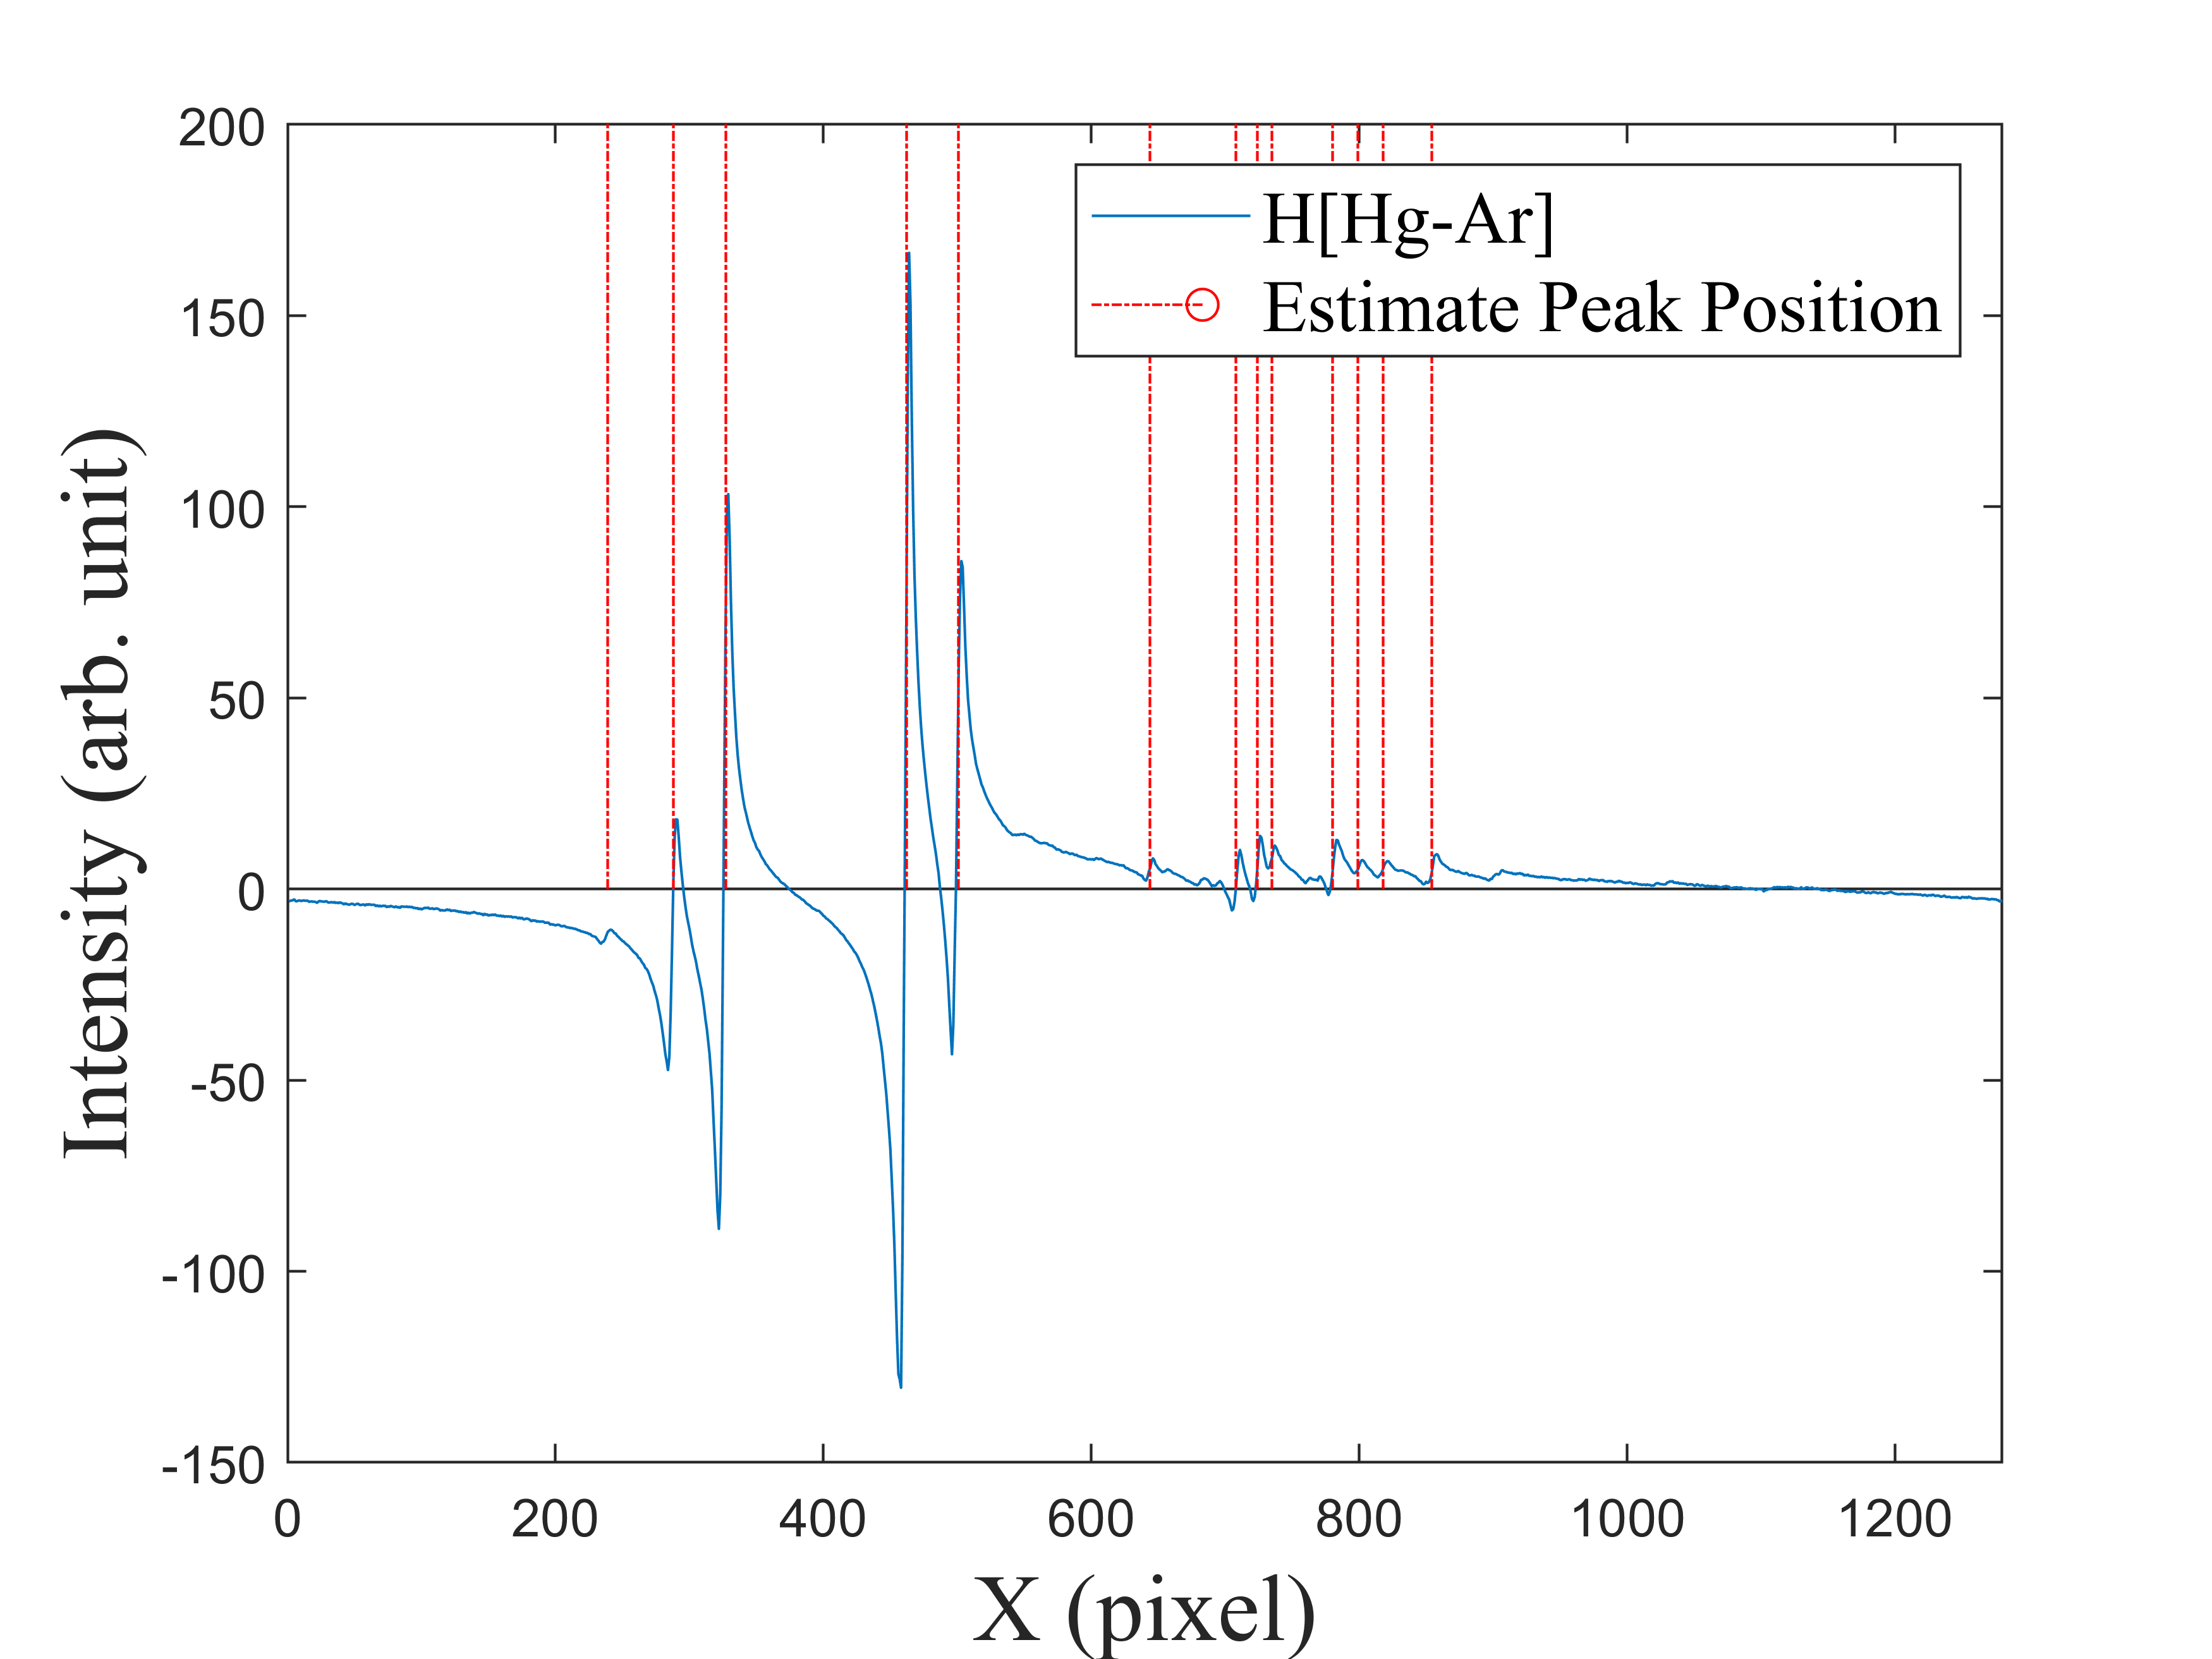
\includegraphics[width=14.5cm]{figures/estimate_peak_position.PNG} %插入图片,[]中设置图片大小,{}中是图片文件名
	\caption{滿足斜率線段之中點即為粗略峰值位置點} %最终文档中希望显示的图片标题
	\label{滿足斜率線段之中點即為粗略峰值位置點} %用于文内引用的标签
\end{figure}
\begin{figure}[H] %H为当前位置,!htb为忽略美学标准,htbp为浮动图形
	\centering %图片居中
	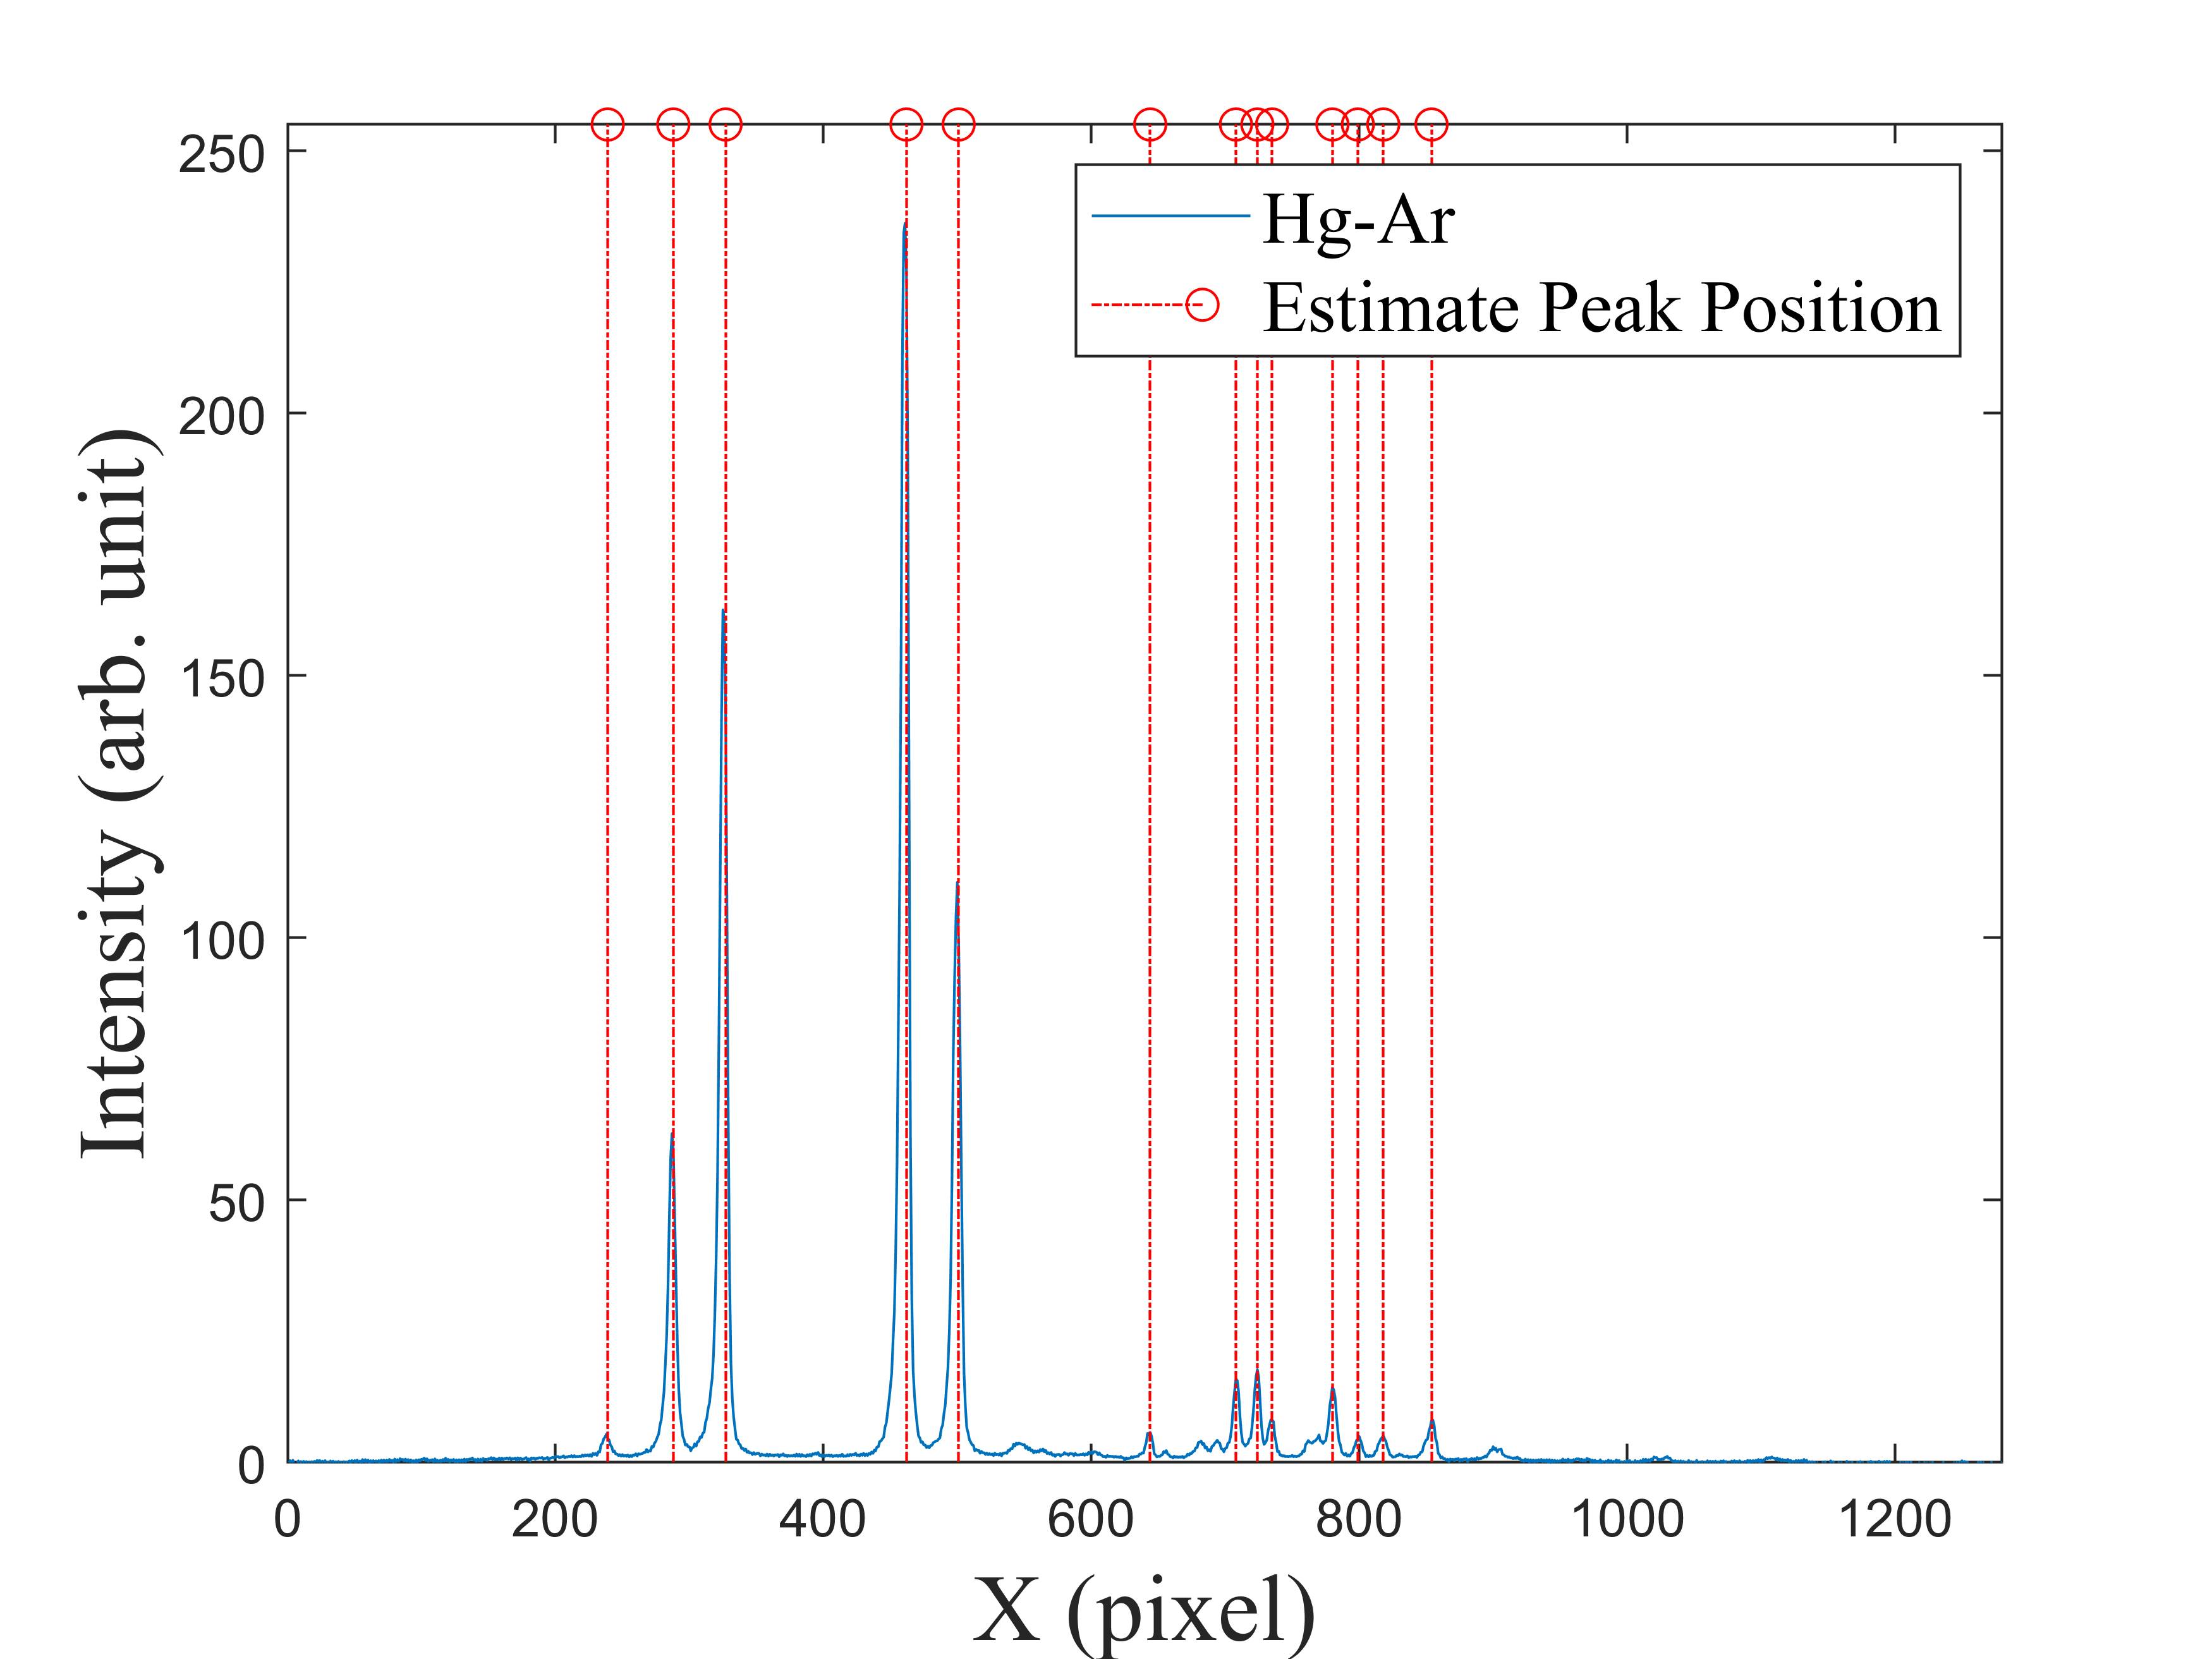
\includegraphics[width=14.5cm]{figures/估測峰值位置.PNG} %插入图片,[]中设置图片大小,{}中是图片文件名
	\caption{粗略峰值位置偵測} %最终文档中希望显示的图片标题
	\label{粗略峰值位置偵測} %用于文内引用的标签
\end{figure}
求得粗略峰值位置後,因應勞倫茲模型擬合需求,需要每一區域中僅有一個波峰,因此為了將數據進行區域分割,本文使用斜率反折法分割區域。
先找出強度平衡後數據的所有區域最大值與最小值,如圖\ref{平衡後汞氬燈波型數據所有區域最大值與最小值}. 所示,再將所有區域最大值與最小值的點由像素大小由小至大排列,再求出所有兩點間斜率,斜率急升前的點與急降後的點,代表為單一波峰的波型起始與結束點,取出所有滿足此斜率行為的點如圖\ref{平衡後汞氬燈波峰數據擬和區域分割點}. 所示。
\begin{figure}[H] %H为当前位置,!htb为忽略美学标准,htbp为浮动图形
	\centering %图片居中
	\vspace{0.8cm}
	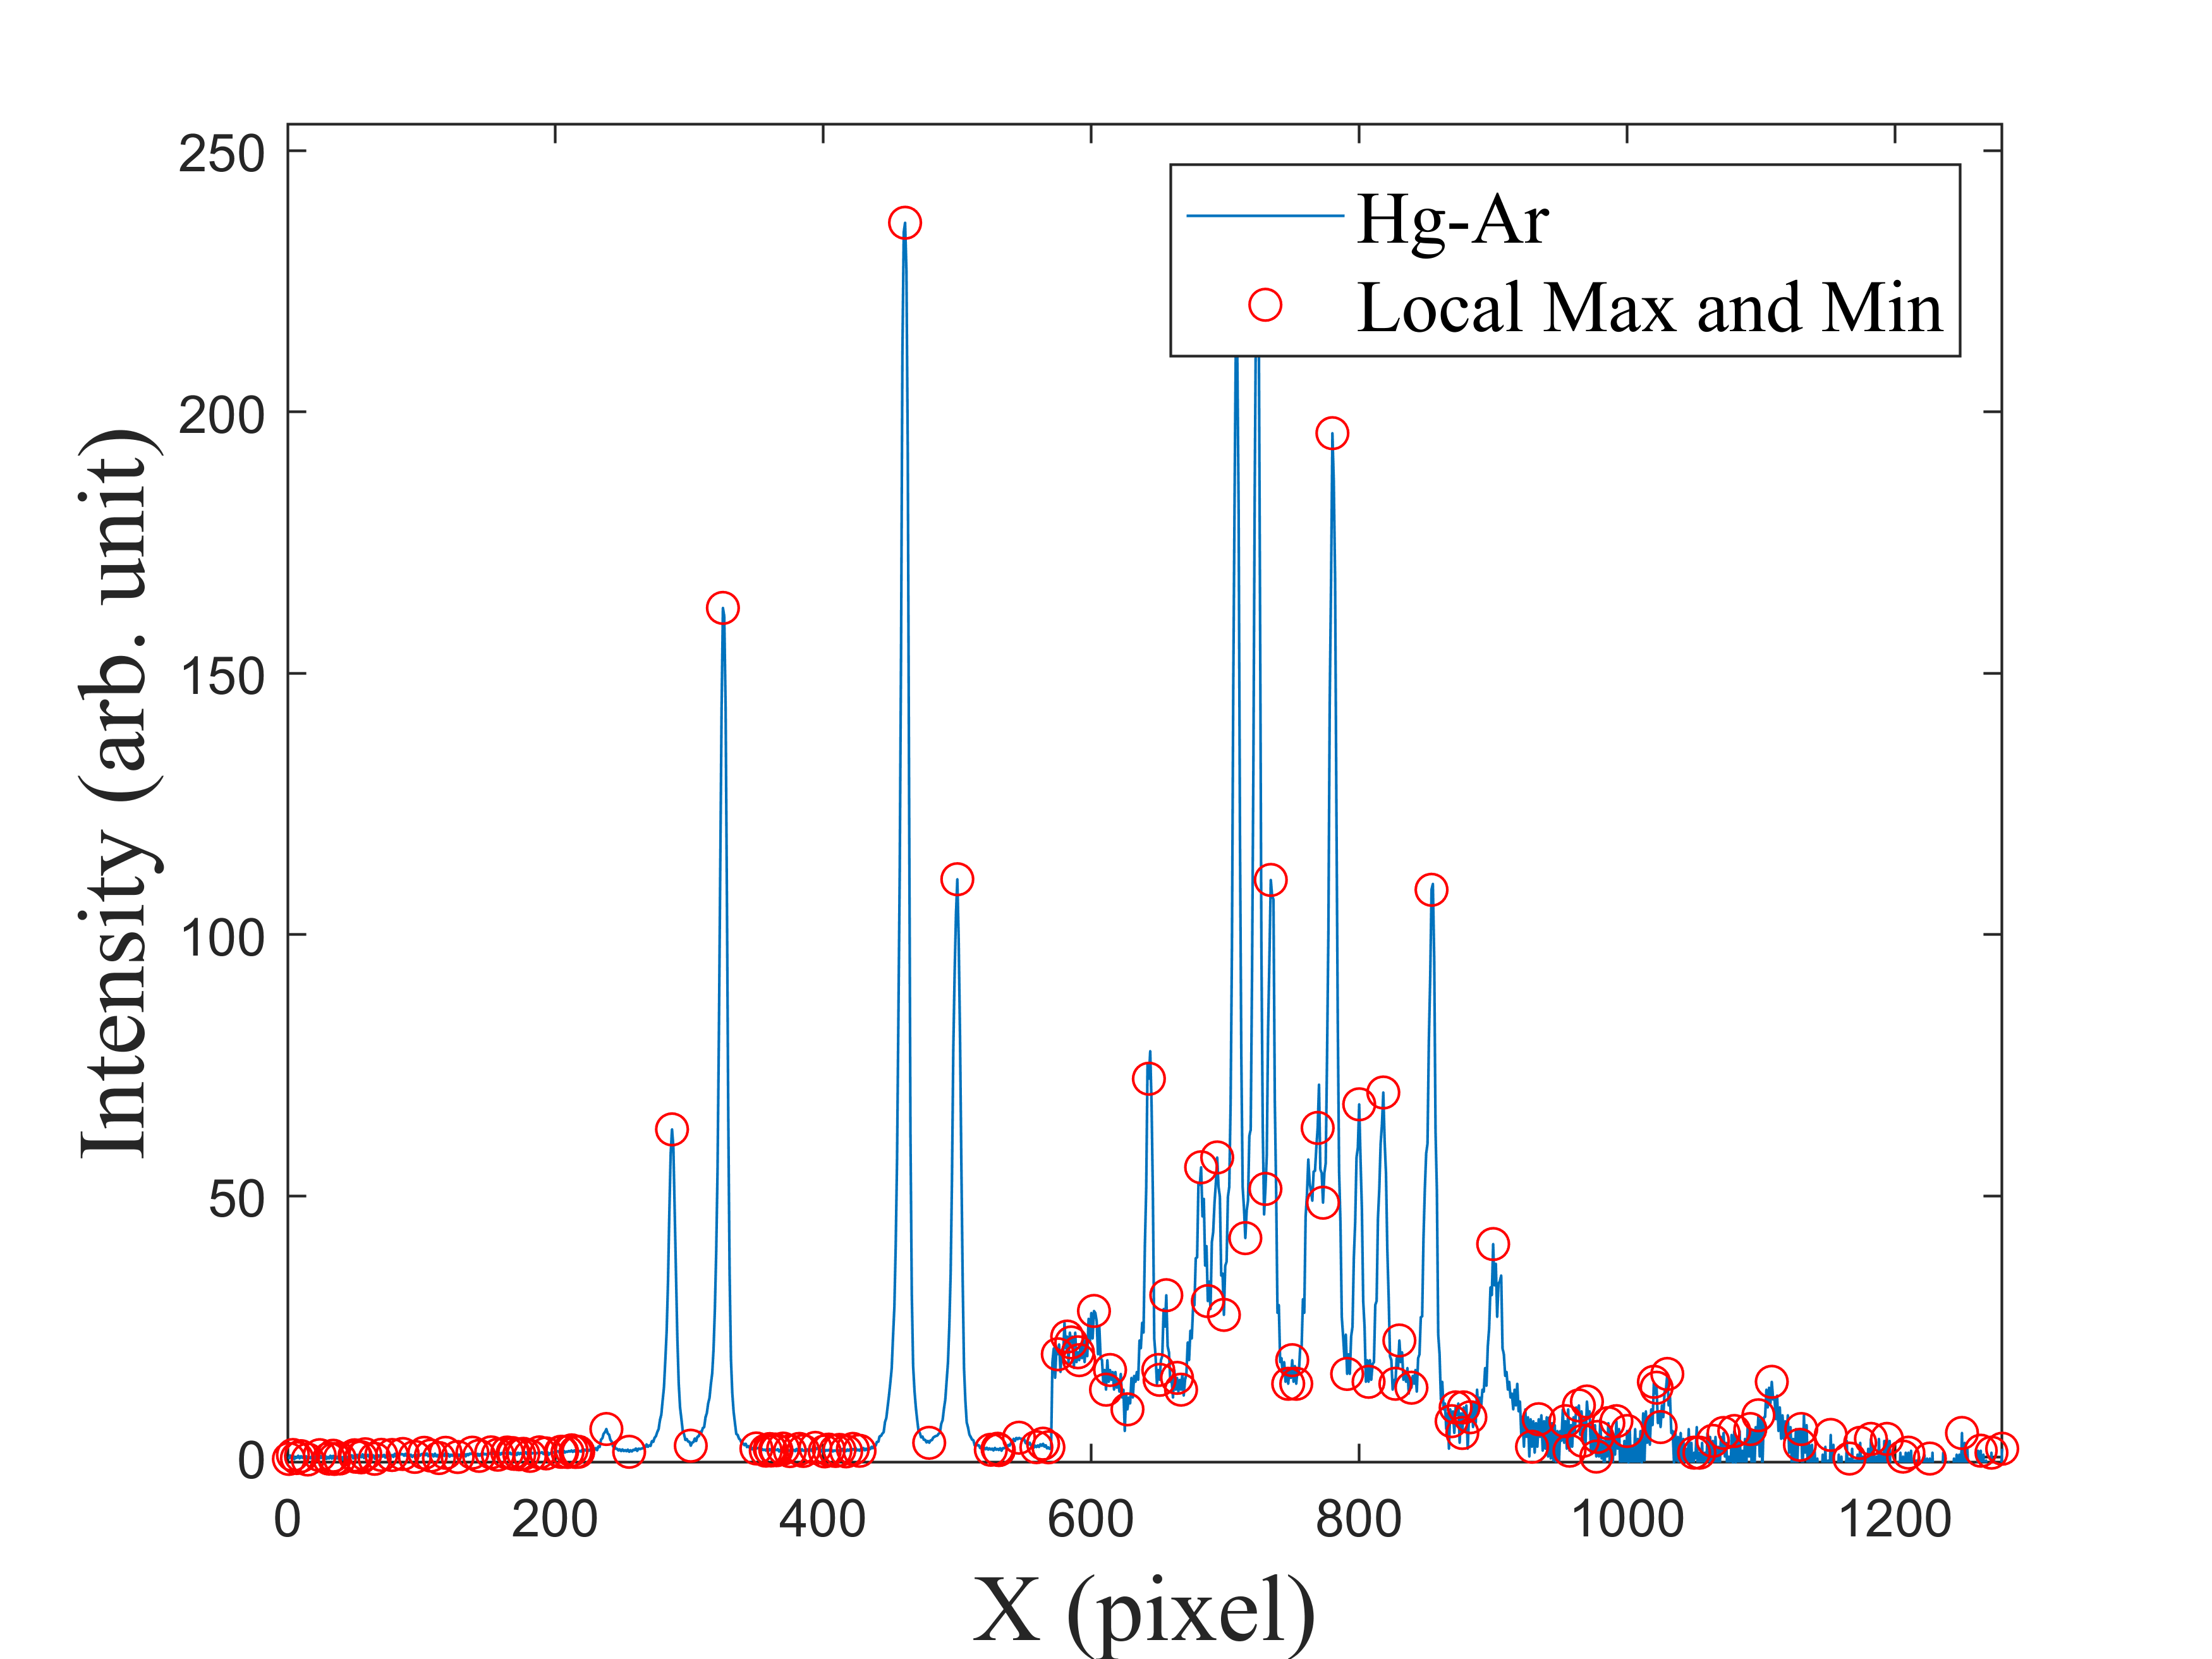
\includegraphics[width=16cm]{figures/combine_local_max_min.png} %插入图片,[]中设置图片大小,{}中是图片文件名
	\caption{平衡後汞氬燈波型數據所有區域最大值與最小值} %最终文档中希望显示的图片标题
	\label{平衡後汞氬燈波型數據所有區域最大值與最小值} %用于文内引用的标签
\end{figure}
\begin{figure}[H] %H为当前位置,!htb为忽略美学标准,htbp为浮动图形
	\centering %图片居中
	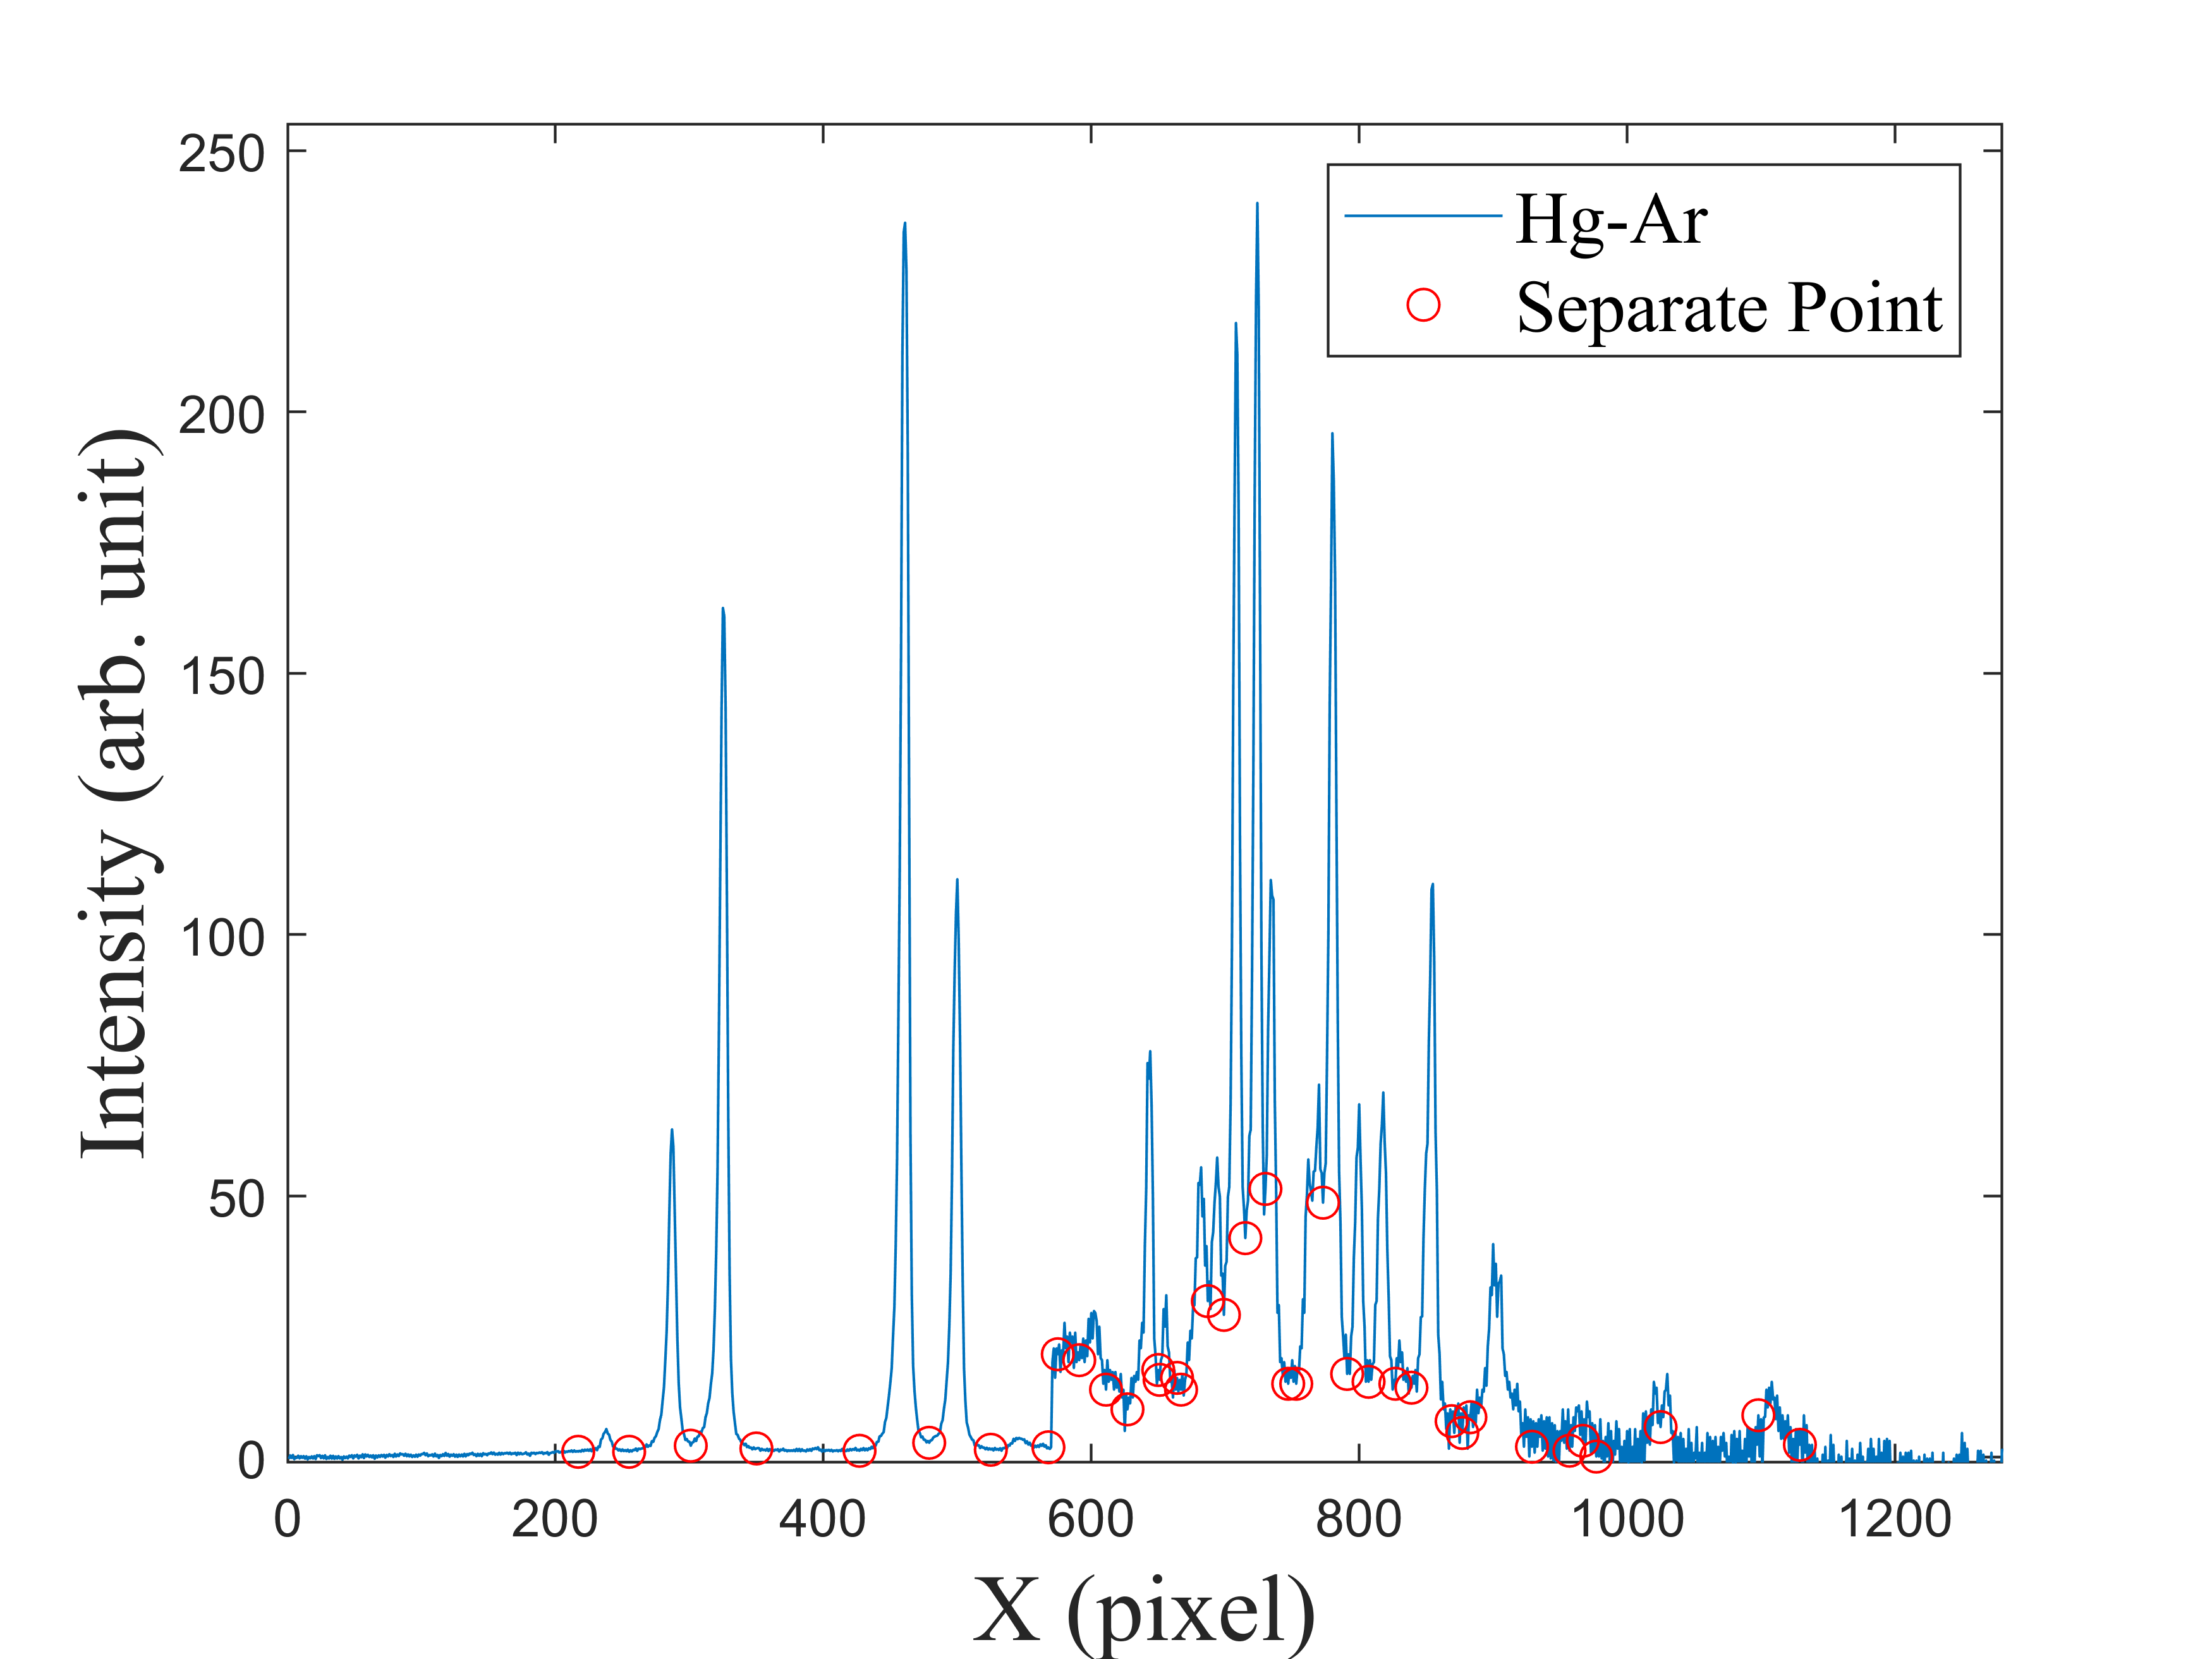
\includegraphics[width=16cm]{figures/combine_sep.png} %插入图片,[]中设置图片大小,{}中是图片文件名
	\caption{平衡後汞氬燈波峰數據擬和區域分割點} %最终文档中希望显示的图片标题
	\label{平衡後汞氬燈波峰數據擬和區域分割點} %用于文内引用的标签
\end{figure}
\par
以這些圖\ref{平衡後汞氬燈波峰數據擬和區域分割點}. 中所求出的分割點對數據進行分割後,如圖\ref{平衡後汞氬燈波峰數據擬和區域分割}. 所示。雖然分割後的分割區域中,並非所有區域數據皆能夠以模型擬合,但含有波峰數據的區域經過數據分割後,滿足第二章所提到模型擬合所需要之先前條件與準備,即所有分割區域中的波峰數據僅剩餘一個波峰,再對分割後區域內數據各自以勞倫茲模型擬合\cite{Lorentz-0},擬合後結果如圖\ref{區域分割後數據以勞倫茲模型擬合結果圖}. 所示。
\begin{figure}[H] %H为当前位置,!htb为忽略美学标准,htbp为浮动图形
	\centering %图片居中
	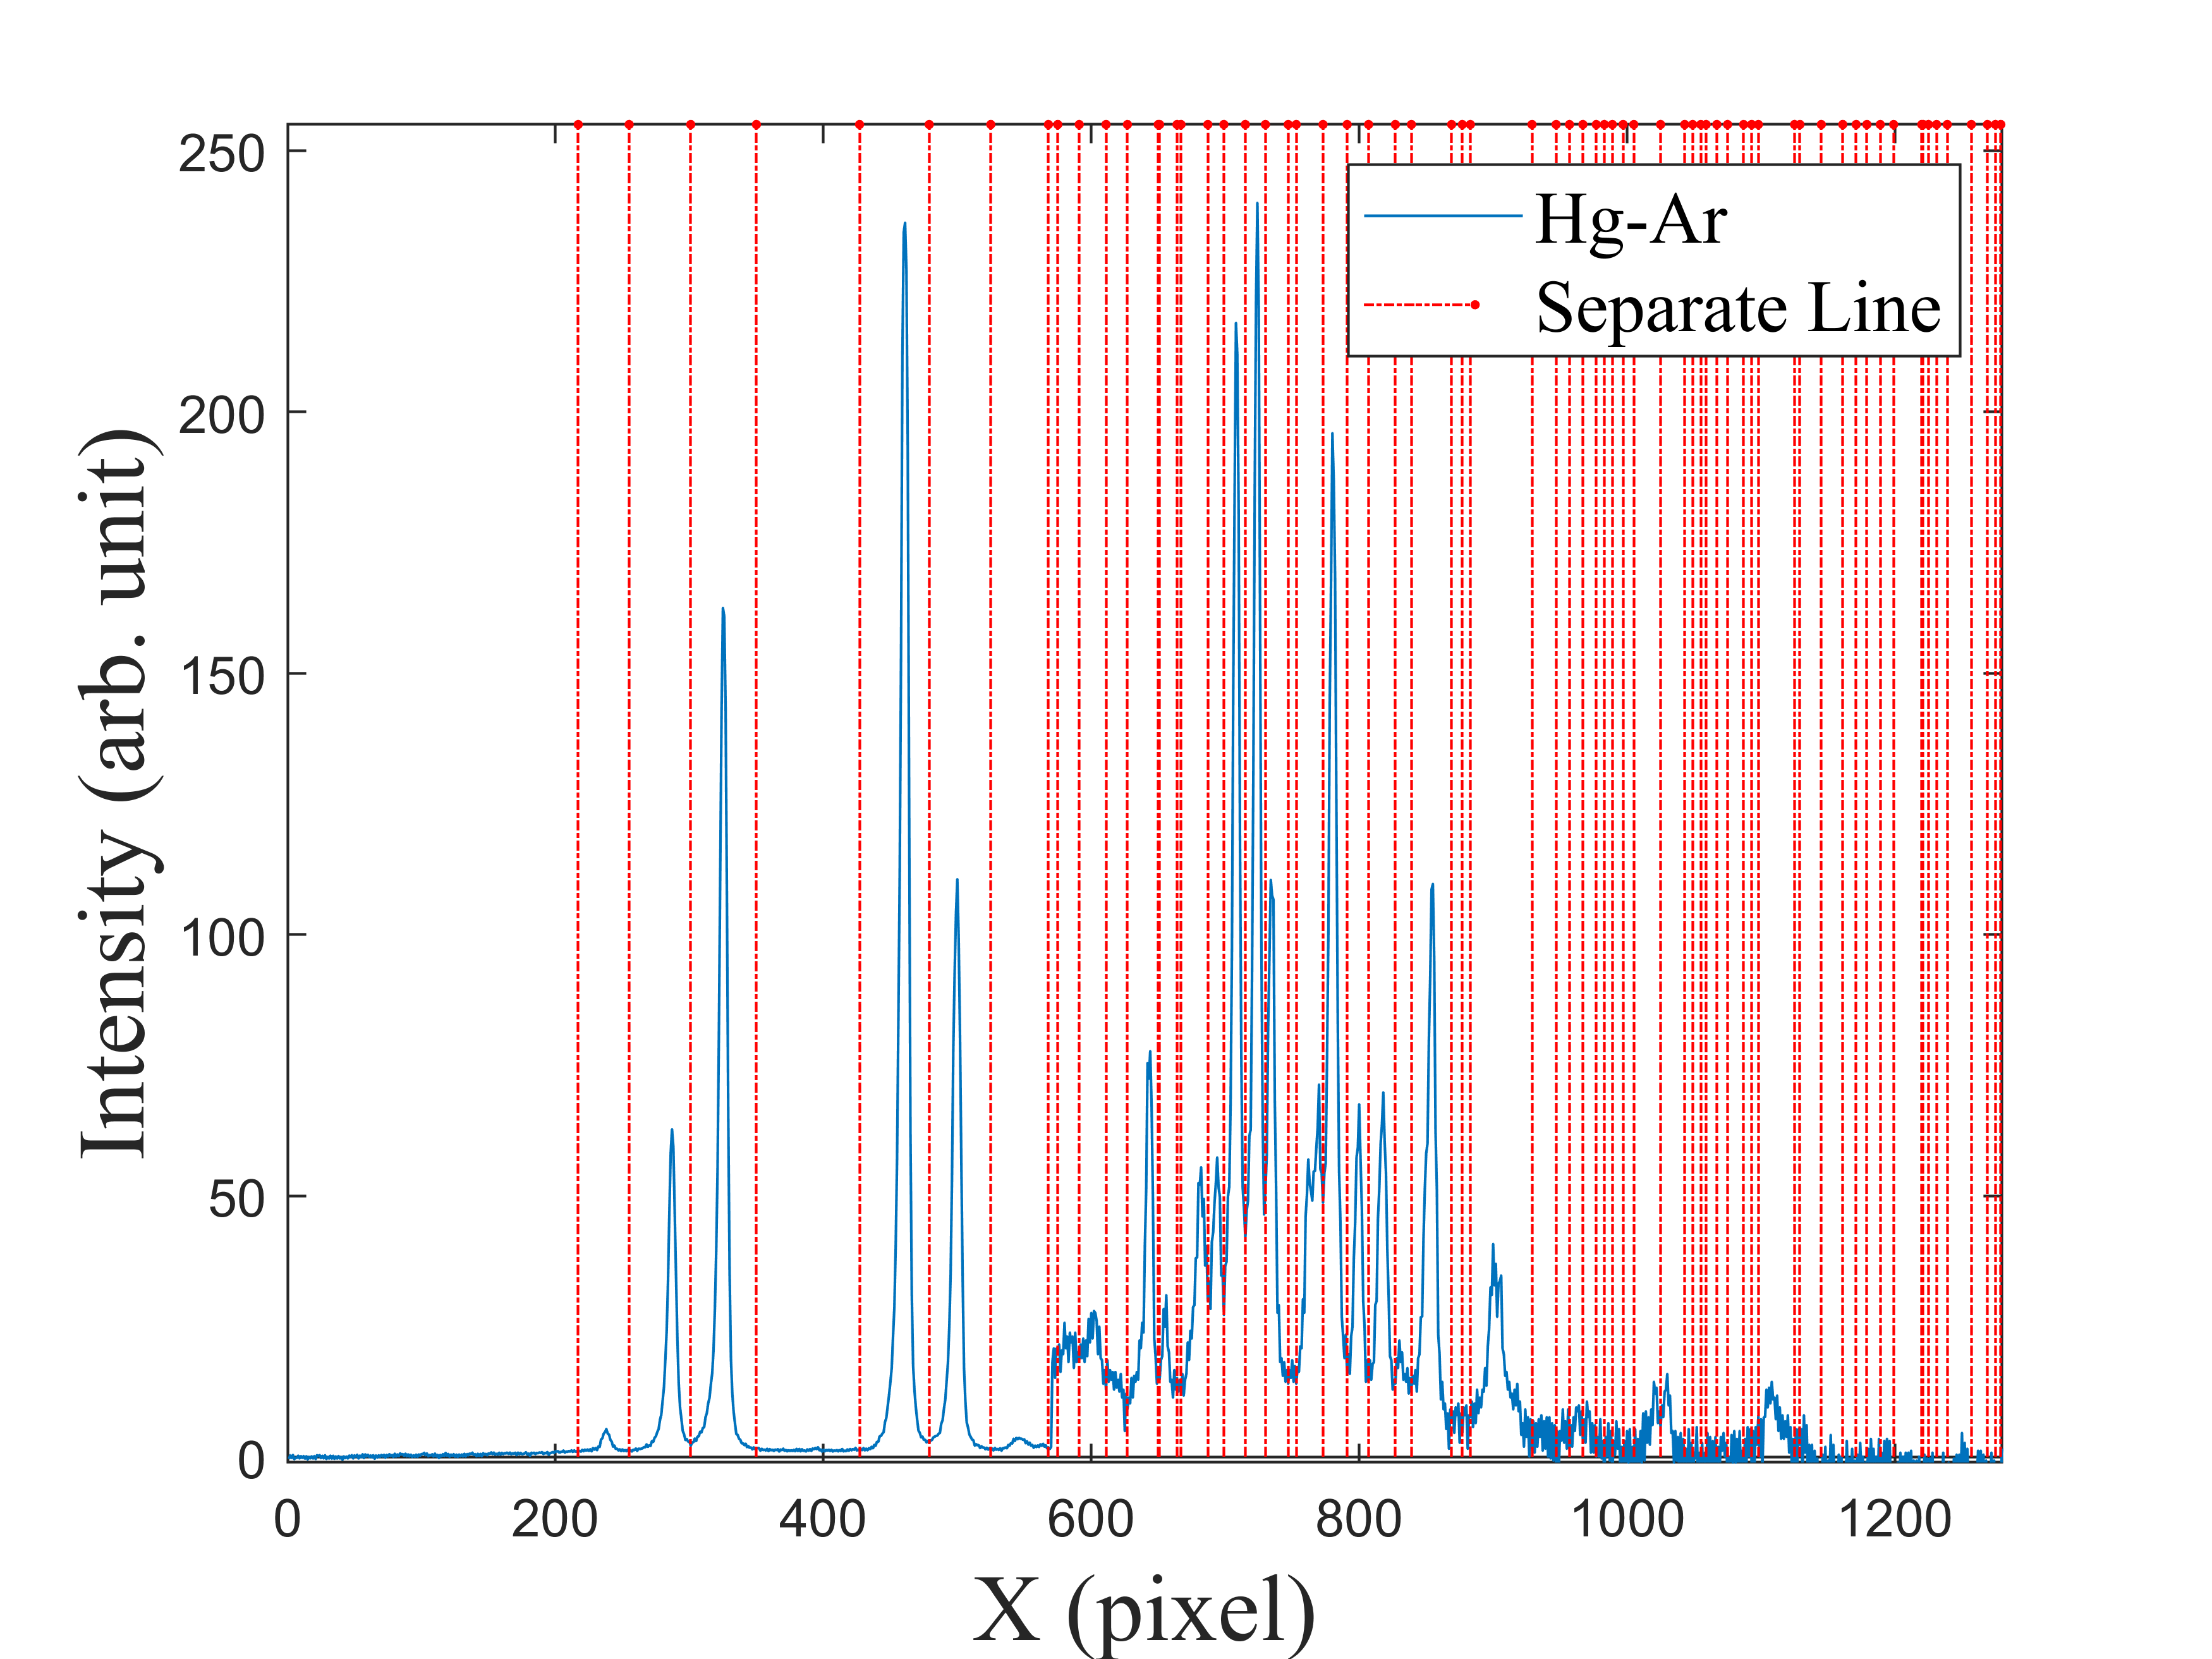
\includegraphics[width=14.5cm]{figures/combine_sep_line600.png} %插入图片,[]中设置图片大小,{}中是图片文件名
	\caption{平衡後汞氬燈波峰數據擬和區域分割} %最终文档中希望显示的图片标题
	\label{平衡後汞氬燈波峰數據擬和區域分割} %用于文内引用的标签
\end{figure}

\begin{figure}[H] %H为当前位置,!htb为忽略美学标准,htbp为浮动图形
	\centering %图片居中
	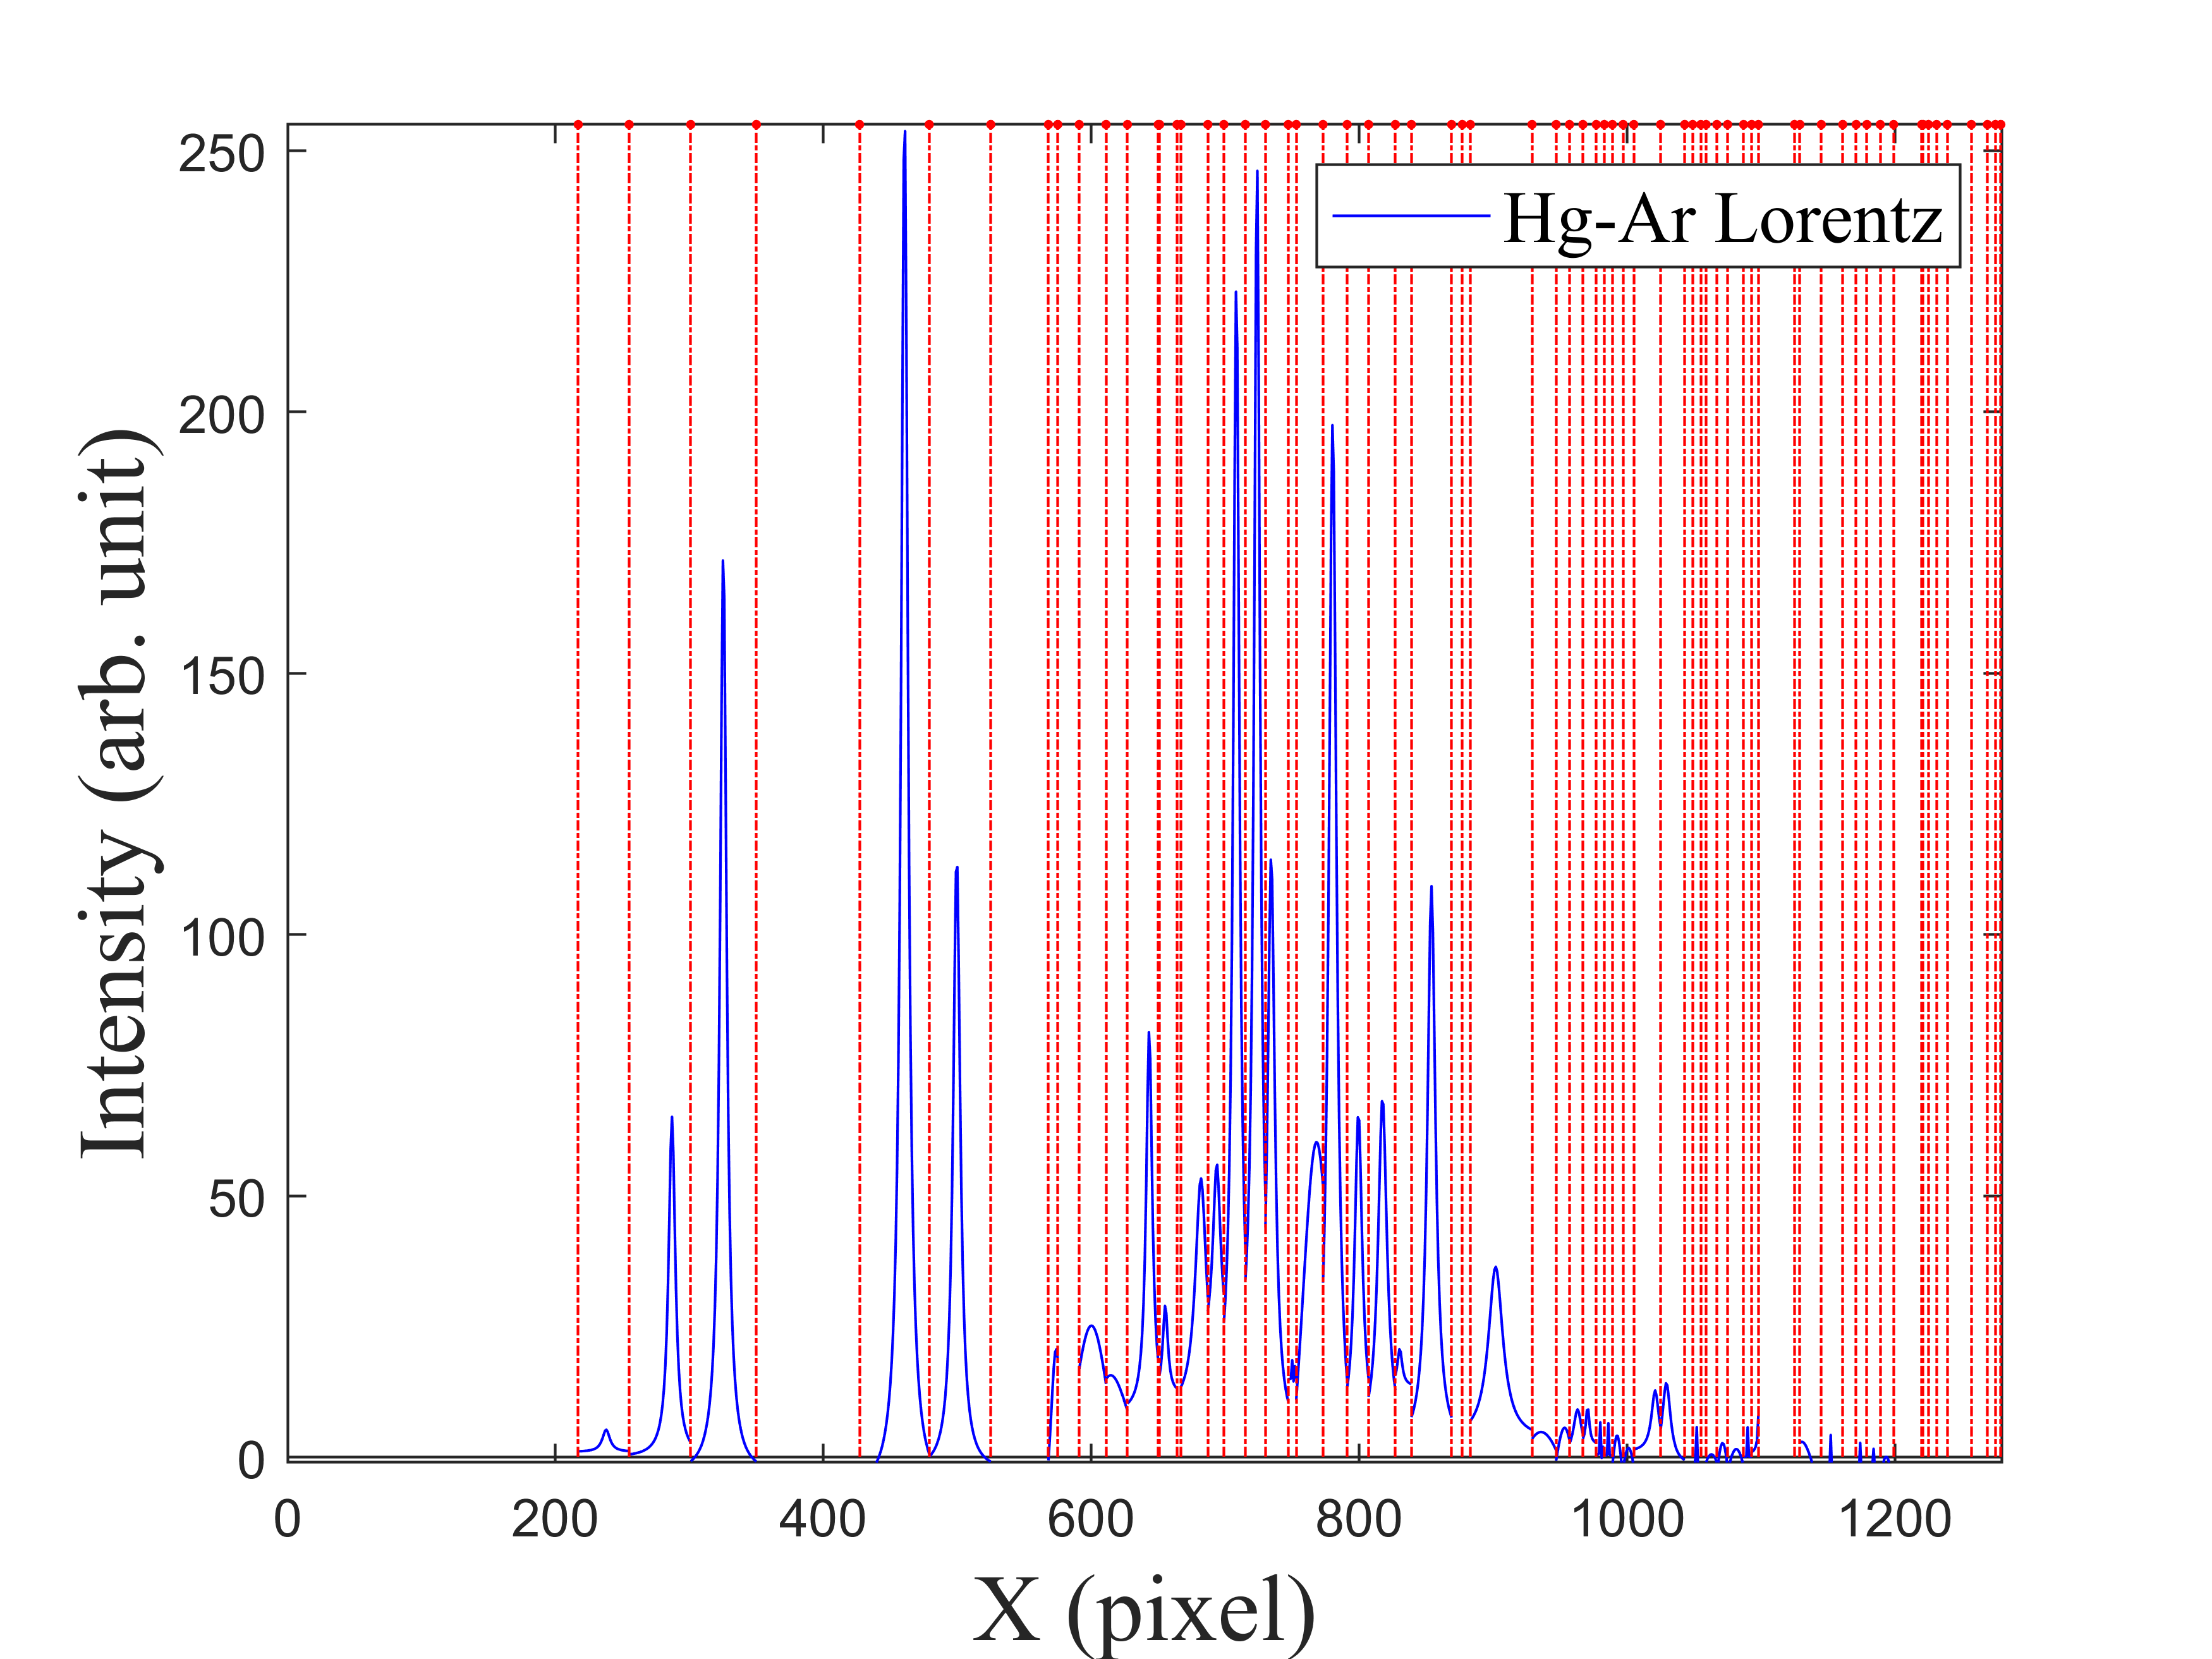
\includegraphics[width=14.5cm]{figures/comebine_hg_ar_lorent.png} %插入图片,[]中设置图片大小,{}中是图片文件名
	\caption{區域分割後數據以勞倫茲模型擬合結果圖} %最终文档中希望显示的图片标题
	\label{區域分割後數據以勞倫茲模型擬合結果圖} %用于文内引用的标签
\end{figure}
再將擬合後獲得的勞倫茲模型參數計算,並將找出的每一個區域中波峰精確的位置,其在勞倫茲模型中的強度,標示於圖\ref{區域分割後數據以勞倫茲模型擬合後且標示出精確波峰位置結果圖}. 中。
\begin{figure}[H] %H为当前位置,!htb为忽略美学标准,htbp为浮动图形
	\centering %图片居中
	\vspace{0.8cm}
	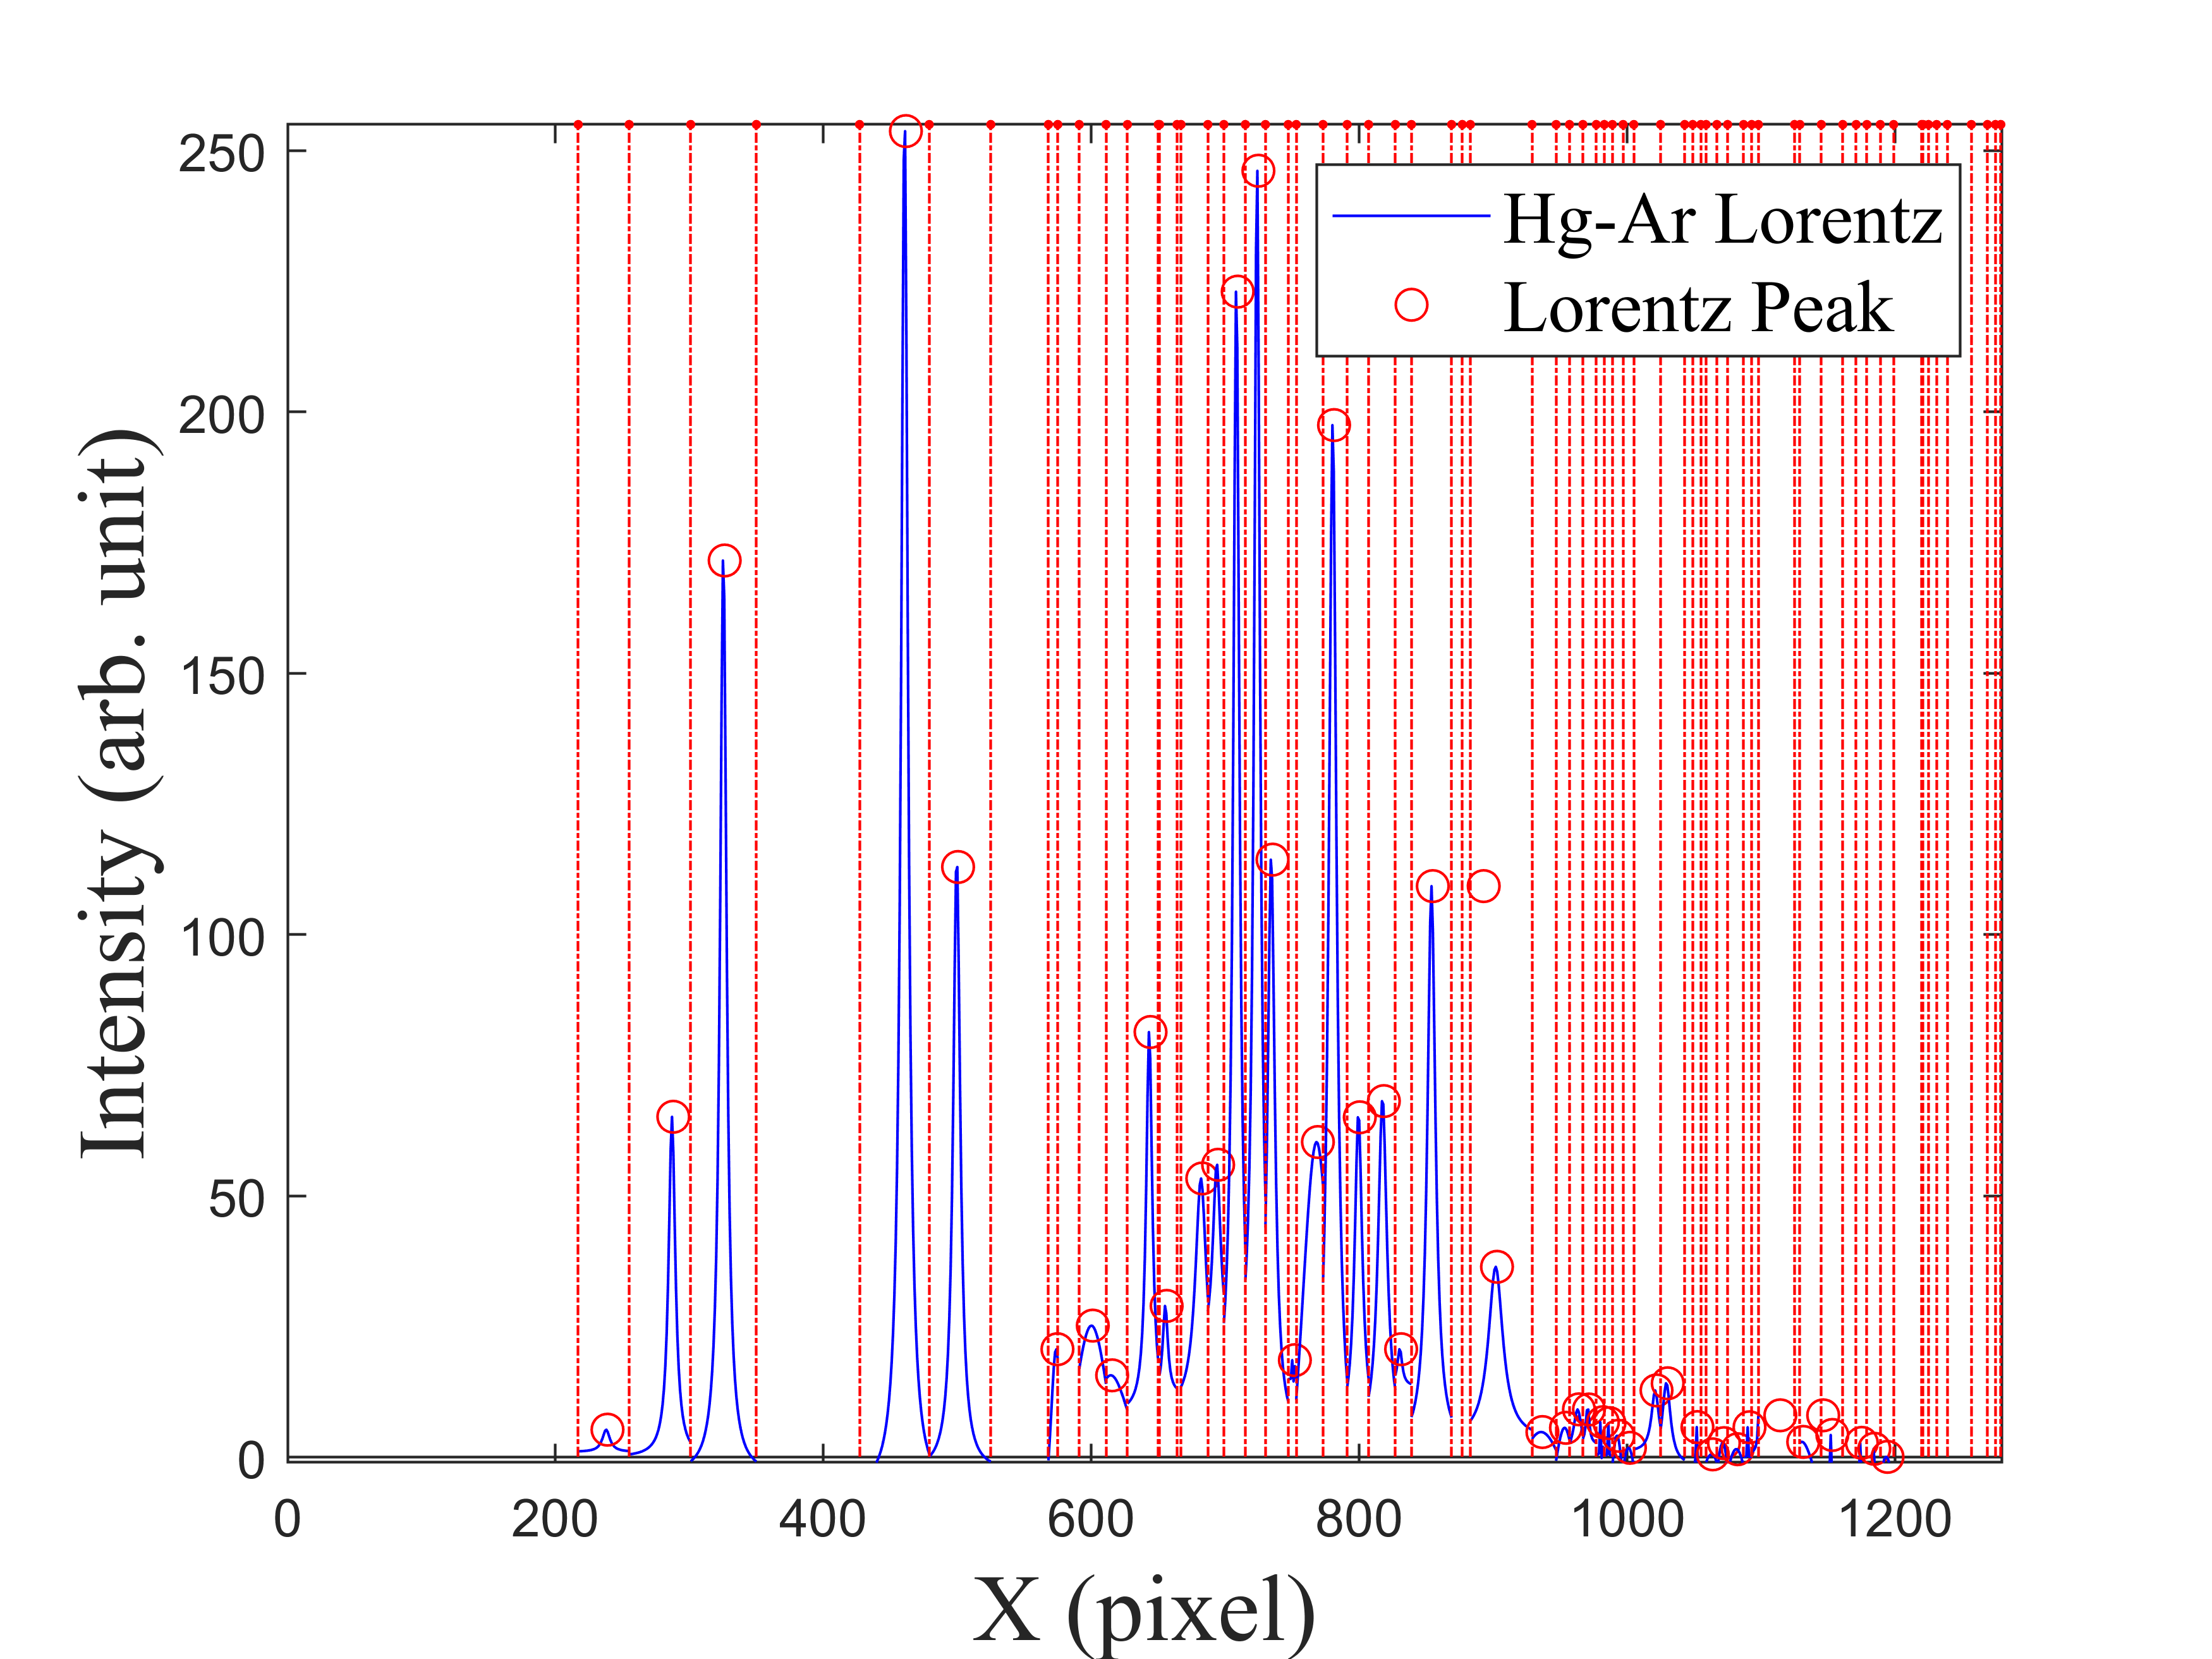
\includegraphics[width=15cm]{figures/comebine_hg_ar_lorent_with_peak.png} %插入图片,[]中设置图片大小,{}中是图片文件名
	\caption{區域分割後數據以勞倫茲模型擬合後且標示出精確波峰位置結果圖} %最终文档中希望显示的图片标题
	\label{區域分割後數據以勞倫茲模型擬合後且標示出精確波峰位置結果圖} %用于文内引用的标签
\end{figure}
由圖\ref{區域分割後數據以勞倫茲模型擬合後且標示出精確波峰位置結果圖}. 中可以看出,因氬燈區域數據強度平衡所造成雜訊放大因素,使得有些雜訊也滿足斜率閥值而被劃分進擬和區域,但由於不是所有數據皆能使用勞倫茲模型函數進行數據擬和,因此造成波峰位置與強度明顯不符合的峰值點,以下稱為無效峰值點,為了移除這些無效峰值點,與雜訊的峰值點,將圖\ref{滿足斜率線段之中點即為粗略峰值位置點}. 中透過原始汞氬燈光譜所找出的粗略峰值位置進行比對,將距離預測峰值最近的峰值點視為有效波峰,其餘波峰皆為無效峰值點,再剔除後所保留下的峰值位置與強度圖於平衡後光譜數據上表示,如圖\ref{區域分割後數據剔除無效峰值點後精確波峰位置結果圖}. 所示。
\begin{figure}[H] %H为当前位置,!htb为忽略美学标准,htbp为浮动图形
	\centering %图片居中
	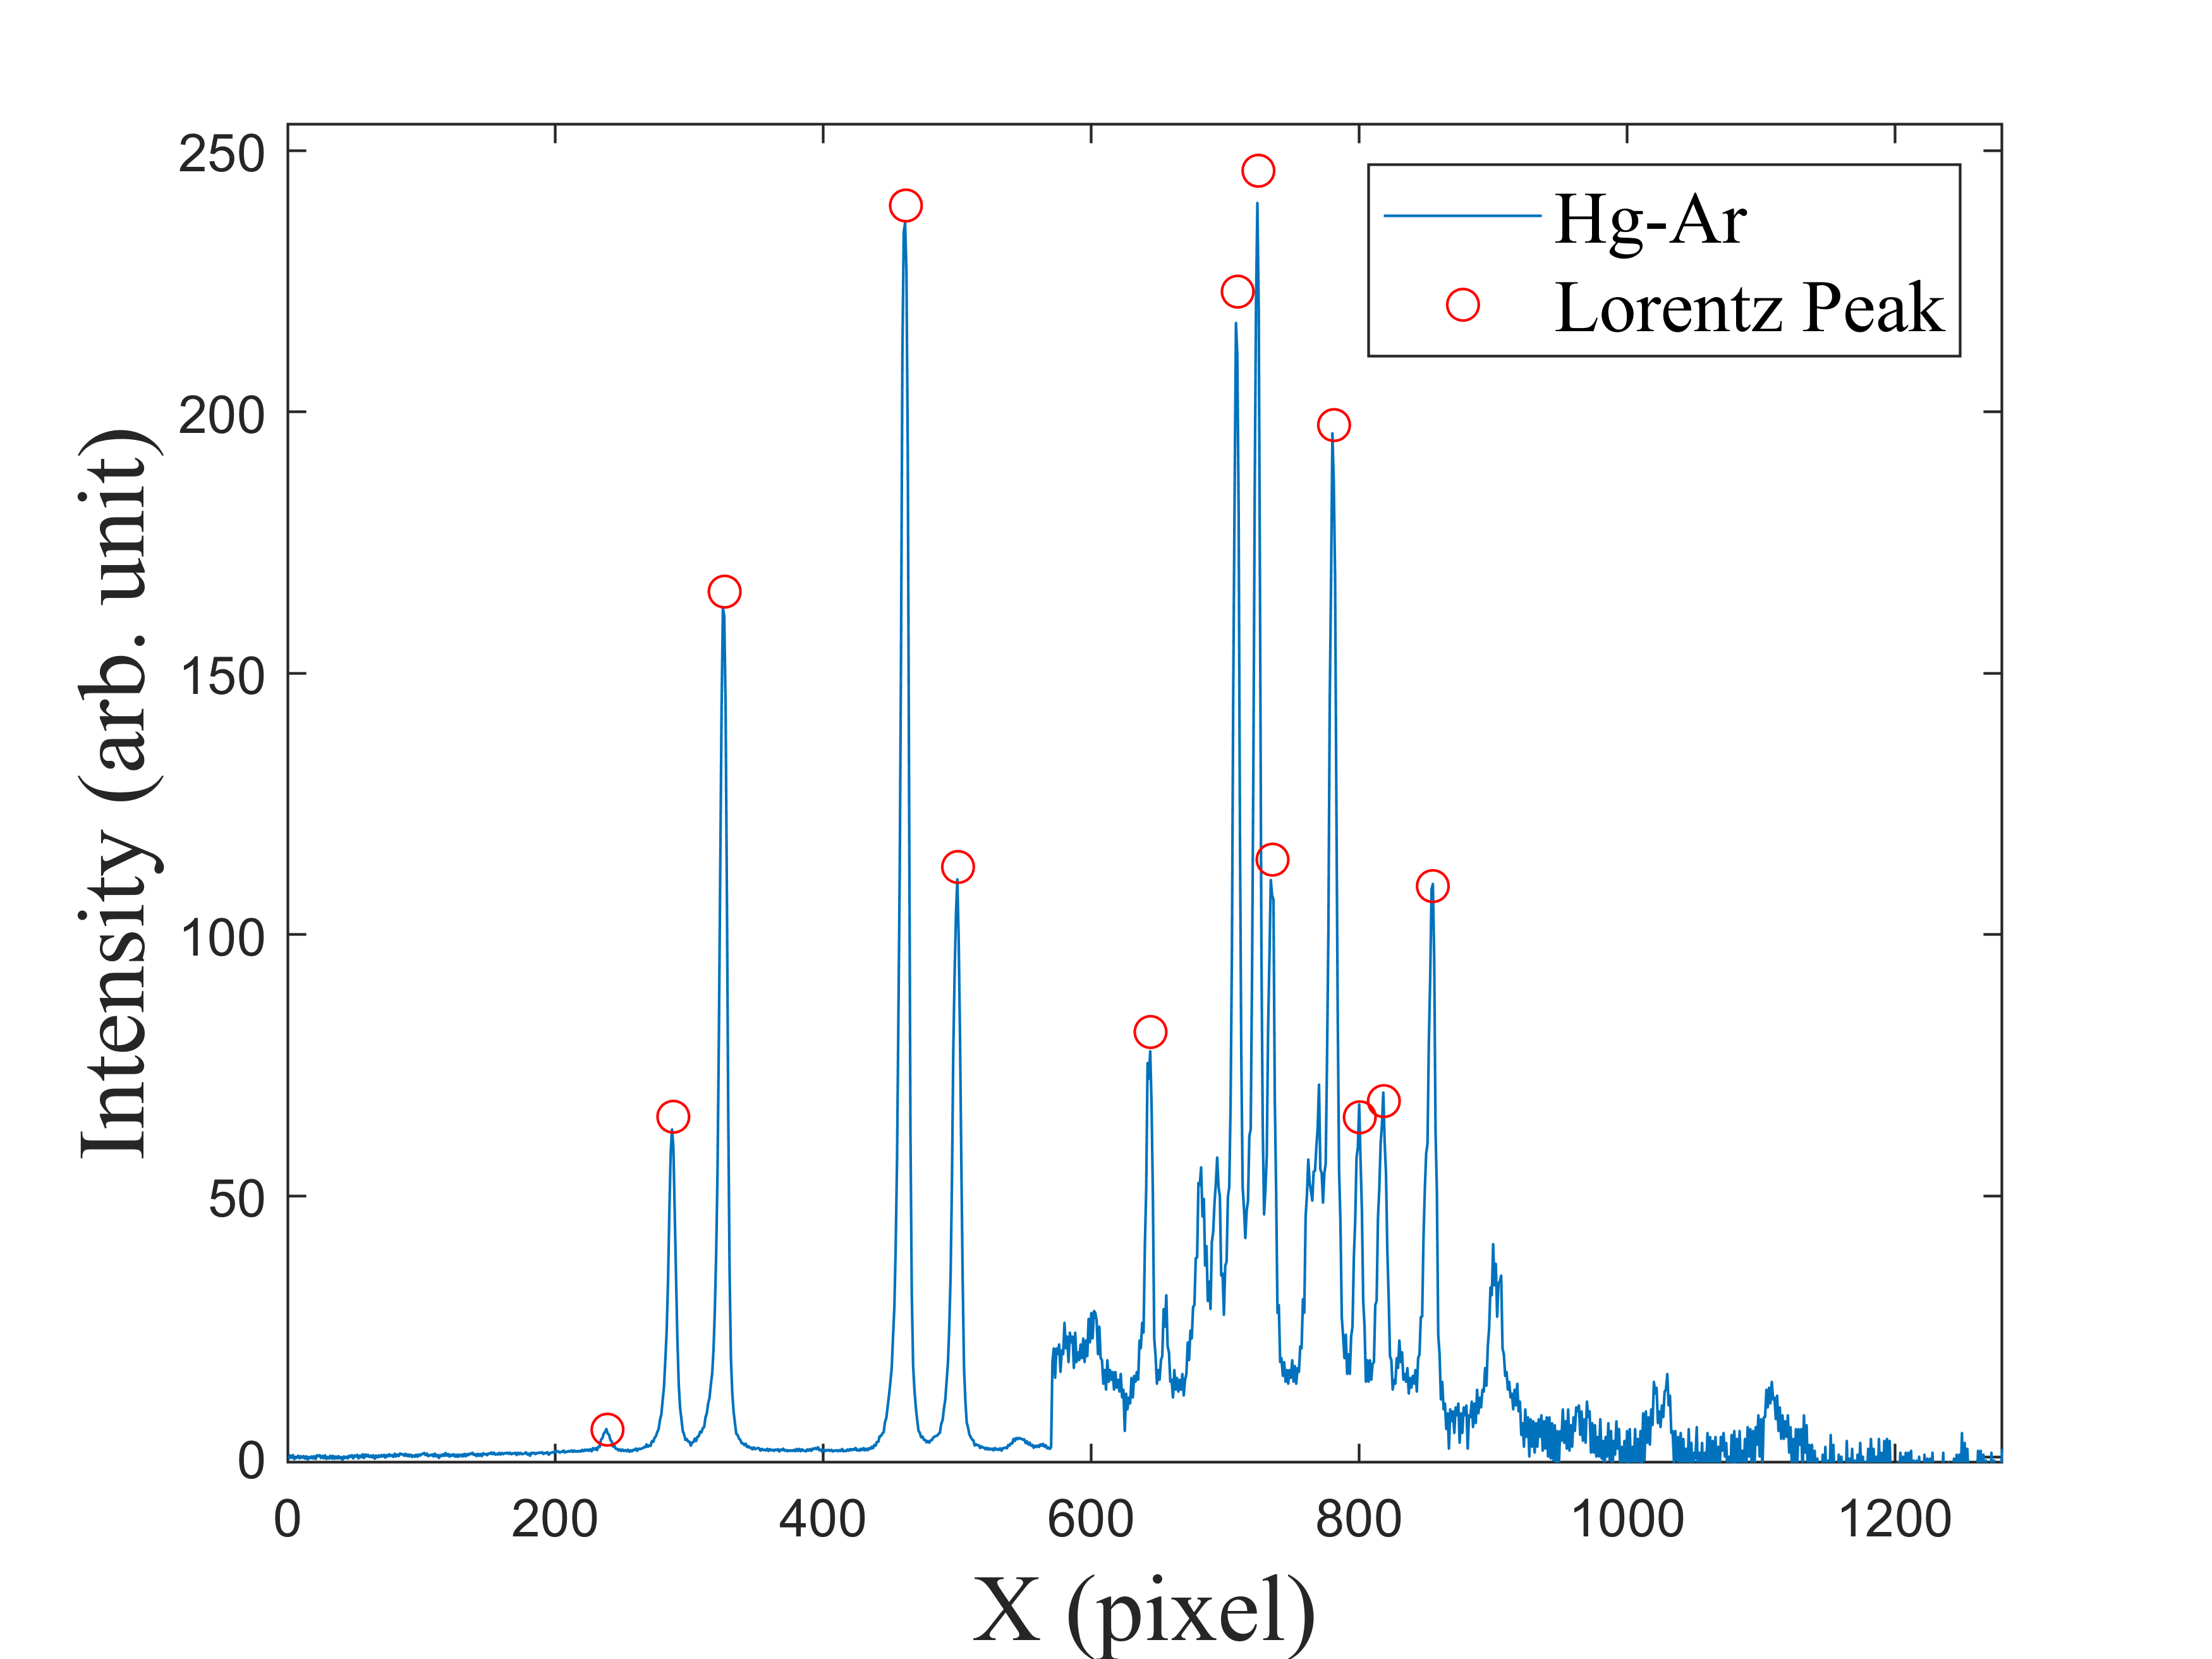
\includegraphics[width=16cm]{figures/與估測峰值比對後峰值.png} %插入图片,[]中设置图片大小,{}中是图片文件名
	\caption{區域分割後數據剔除無效峰值點後精確波峰位置結果圖} %最终文档中希望显示的图片标题
	\label{區域分割後數據剔除無效峰值點後精確波峰位置結果圖} %用于文内引用的标签
\end{figure}
在初步去除所有無效峰值點後,透過以勞倫茲模型擬合後找出的精確峰值位置與其強度及半高全寬數據如表\ref{汞氬燈高斯擬合求得參數表}. 所示。
\newpage
\begin{center}
	\vspace{0.8cm}
	\captionof{table}{汞氬燈高斯擬合求得參數表}\label{汞氬燈高斯擬合求得參數表}
\begin{tabularx}{\textwidth}{m{0.2\textwidth}<{\centering}m{0.2\textwidth}<{\centering}m{0.25\textwidth}<{\centering}m{0.2\textwidth}<{\centering}}
	\hline\hline
	光源            & 峰值位置(pixel) & 強度 & 半高全寬(pixel) \\
	\hline
	\multirow{5}{*}{汞燈 }
	&238.8276368&    5.270303917& 5.2307\\
	&287.9697699&	65.14440122& 5.7020\\
	&326.3158442&	171.58091  & 5.6381\\
	&461.6027204&	253.7391256& 5.1501\\
	&500.5412743&	112.9370475& 5.8473\\
	\hline
	\multirow{8}{*}{氬燈 }
	&644.2331809&	81.36141267& 3.8002\\
	&709.2949685&	223.0211324& 3.9613\\
	&724.7514346&	246.1550526& 3.8504\\
	&735.3158606&	114.3412062& 3.2691\\
	&781.2286706&	197.4903351& 2.9736\\
	&800.4412516&	65.04398951& 3.9324\\
	&818.4181357&	68.13802375& 4.1103\\
	&854.9459689&	109.2759383& 4.8757\\                     
	\hline\hline
\end{tabularx}
\vspace{10pt}
\end{center}
\par 
由表\ref{汞氬燈高斯擬合求得參數表}. 及圖\ref{區域分割後數據剔除無效峰值點後精確波峰位置結果圖}. 可知,雖以預測峰值位置除去多餘峰值點,但仍不全然為目標波峰,在此階段本文利用光譜波峰位置與強度雖然每次量測都不同,但峰值間彼此的距離是相同的特性。當在以相同影像感測器情況下,現已知汞燈區的最後一個波峰像素位置與氬燈兩目標波峰分別相差225個像素與280個像素,留下與此距離最接近的兩個氬燈區波峰後,最後所有目標波峰的準確波峰位置與強度如圖\ref{最終目標波峰的峰值位置與強度結果圖}. 所示,詳細資訊如表\ref{最終目標波峰參數表}. 所示,並將資訊紀錄於程式暫存記憶體中。
\begin{figure}[H] %H为当前位置,!htb为忽略美学标准,htbp为浮动图形
	\centering %图片居中
	%\setlength{\abovecaptionskip}{1cm}
	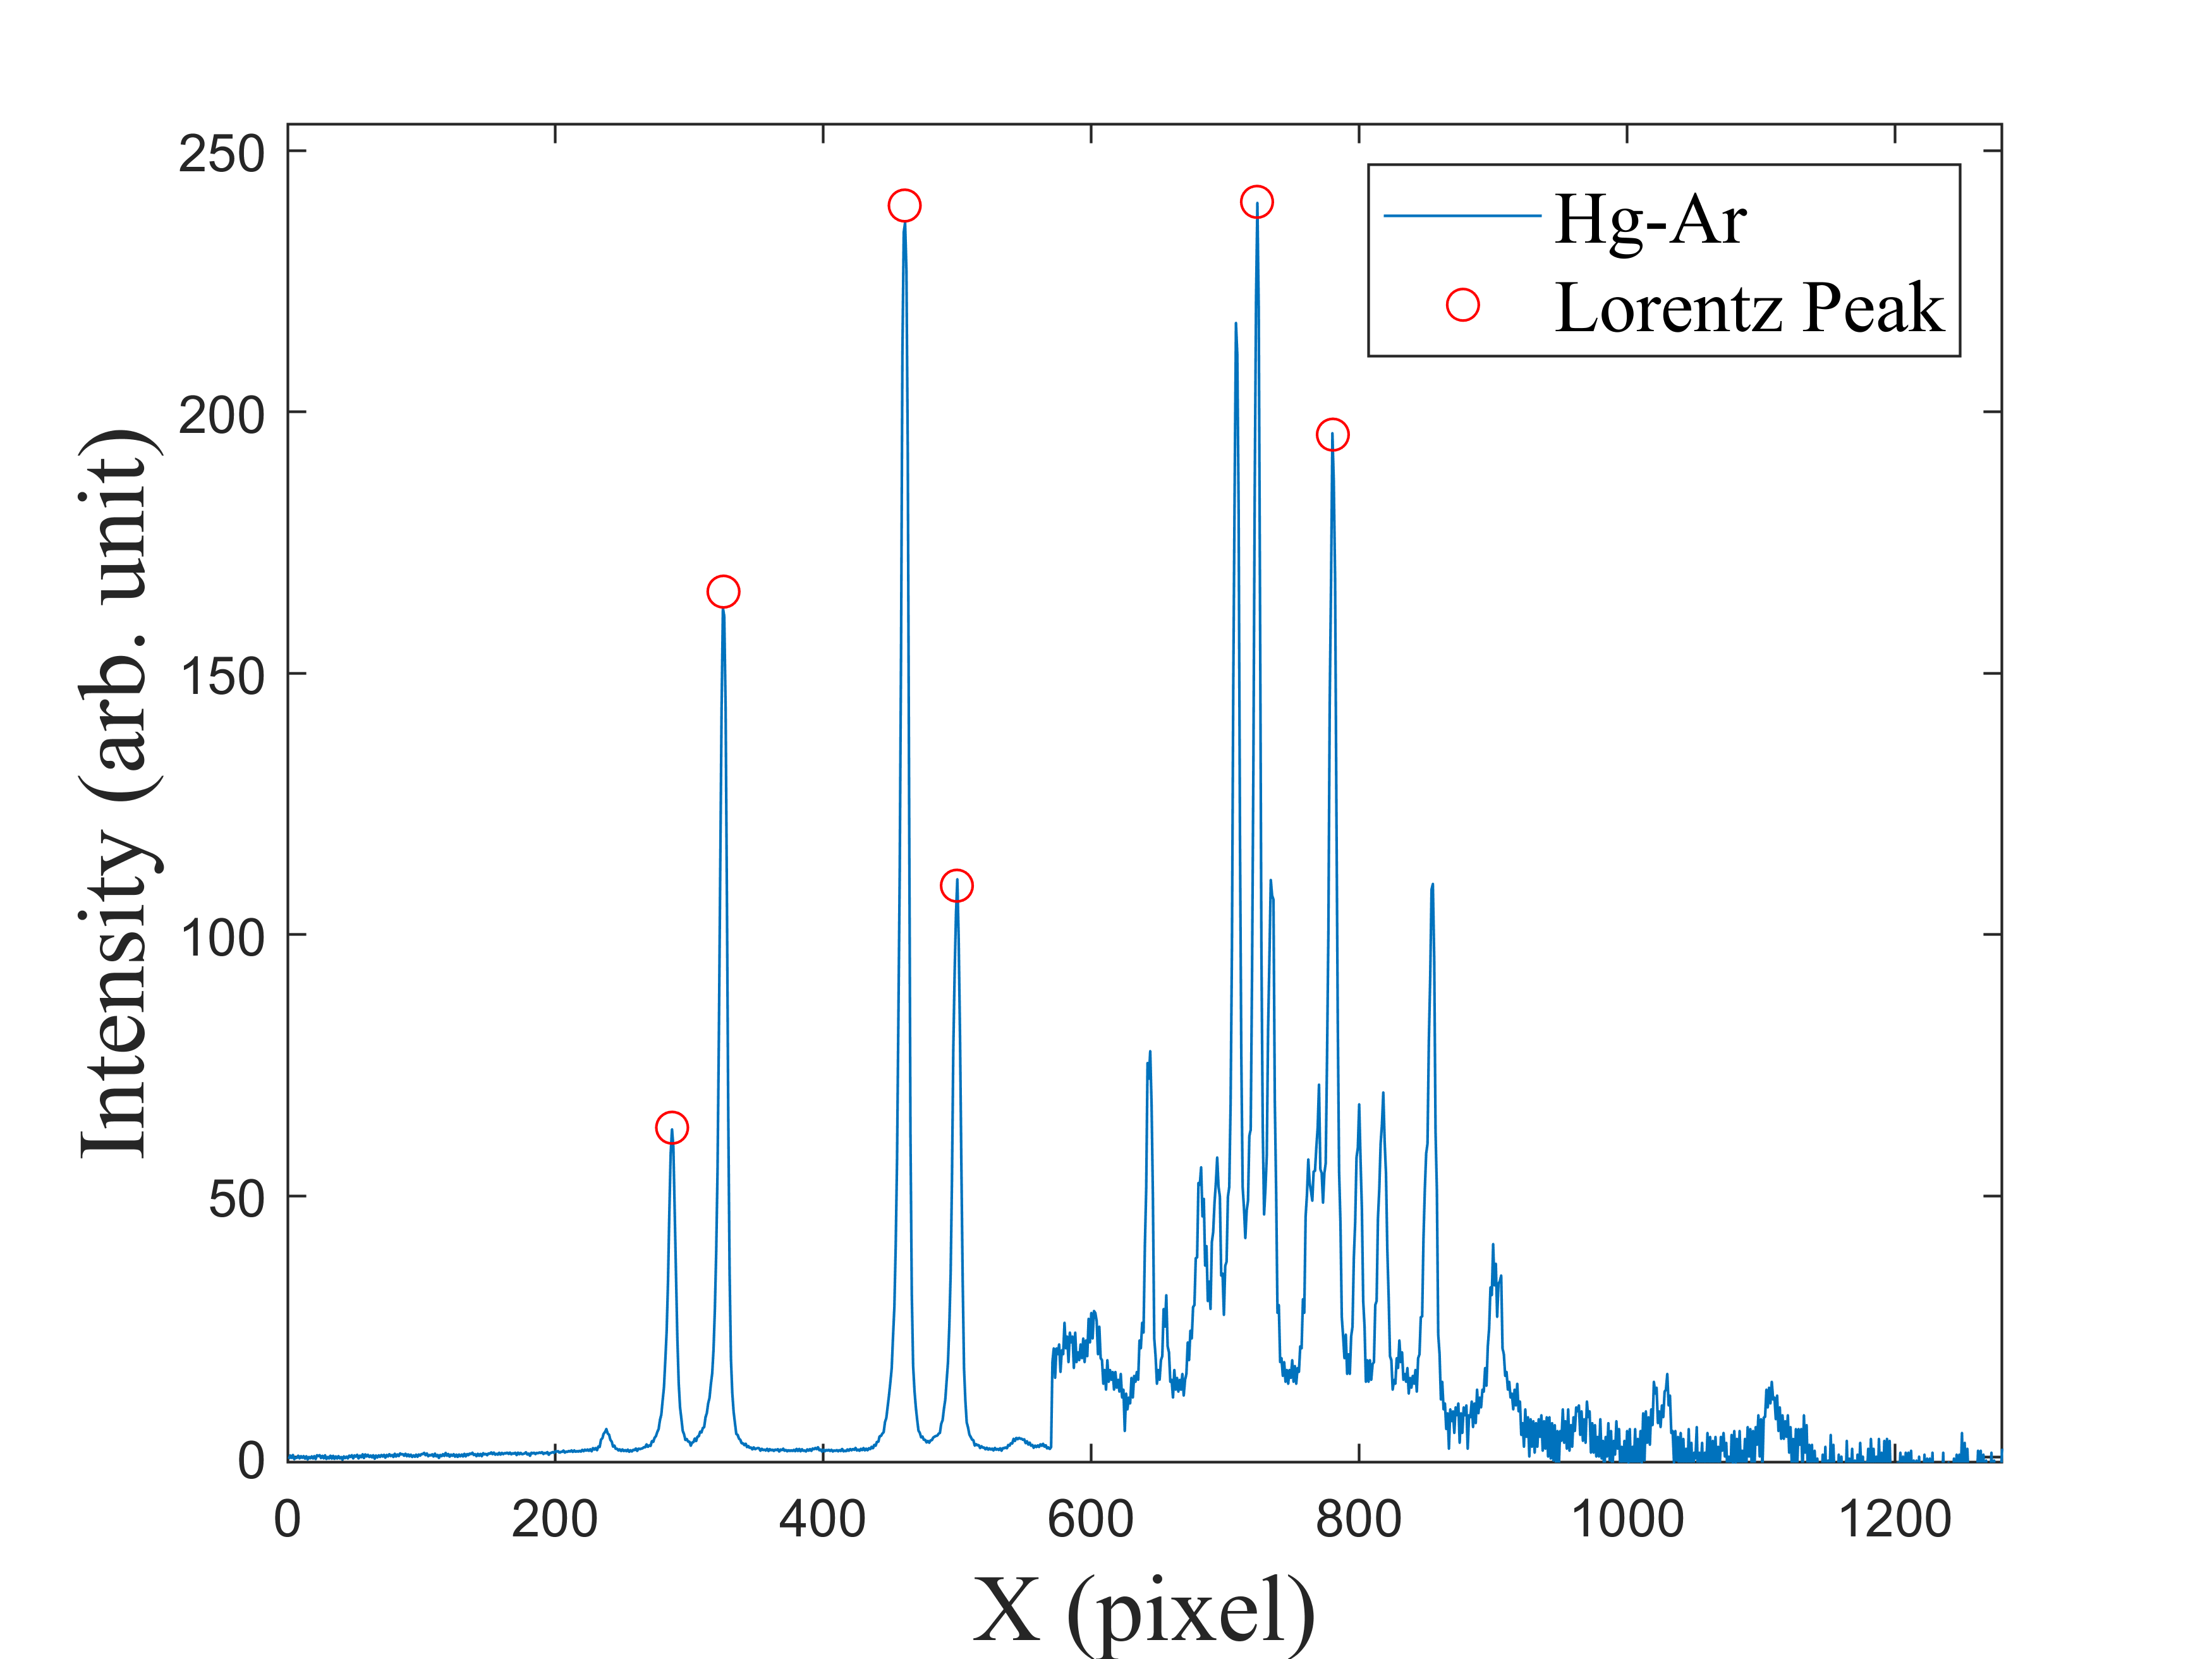
\includegraphics[width=16cm]{figures/comebine_hg_ar_最終PEAK.png} %插入图片,[]中设置图片大小,{}中是图片文件名
	\caption{最終目標波峰的峰值位置與強度結果圖} %最终文档中希望显示的图片标题
	\label{最終目標波峰的峰值位置與強度結果圖} %用于文内引用的标签
\end{figure}

\begin{center}
\vspace{0.8cm}
\captionof{table}{最終目標波峰參數表}\label{最終目標波峰參數表}
\begin{tabularx}{\textwidth}{m{0.2\textwidth}<{\centering} m{0.21\textwidth}<{\centering} m{0.25\textwidth}<{\centering}c}
	\hline\hline
	光源            & 峰值位置(pixel) & 強度 & 半高全寬(pixel) \\
	\hline
    \multirow{4}{*}{汞燈 }
    &287.9697699&	65.14440122& 5.7020\\
    &326.3158442&	171.58091  & 5.6381\\
    &461.6027204&	253.7391256& 5.1501\\
    &500.5412743&	112.9370475& 5.8473\\
    \hline
    \multirow{2}{*}{氬燈 }
    &724.7514346&	246.1550526& 3.8504\\
    &781.2286706&	197.4903351& 2.9736\\                   
	\hline\hline
\end{tabularx}
\end{center}
\subsection{單雷射波峰位置偵測}
相對於汞氬燈源來說,雷射光源十分的不穩定,燈源跳動造成AutoScaling完成後的光源無法穩定在同一強度上,使得無法精確取到強度為AutoScaling完成時的數據,所幸雷射光源波型單調,波峰僅有雷射光源與其二階光\cite{diffraction-2nd-Light}此二波峰,且兩者強度相差極大,因此透過強度閥值便可以過濾掉二階光產生的波峰。\par
當一雷射光源輸入且已經由AutoScaling調整至適當強度後,波型如圖\ref{雷射光譜強度波型圖}. 所示,雷射波形於表\ref{光源介紹表}. 說明,其特定波長能量放大所產生之光束,能以勞倫茲模型擬合逼近,因此在進行雷射波峰位置偵測時,將採用勞倫茲擬合來找出準確波峰位置、半高全寬與強度值。
\begin{figure}[H] %H为当前位置,!htb为忽略美学标准,htbp为浮动图形
	\centering %图片居中
	\vspace{0.8cm}
	%\setlength{\abovecaptionskip}{1cm}
	\setlength{\abovecaptionskip}{0.cm}
	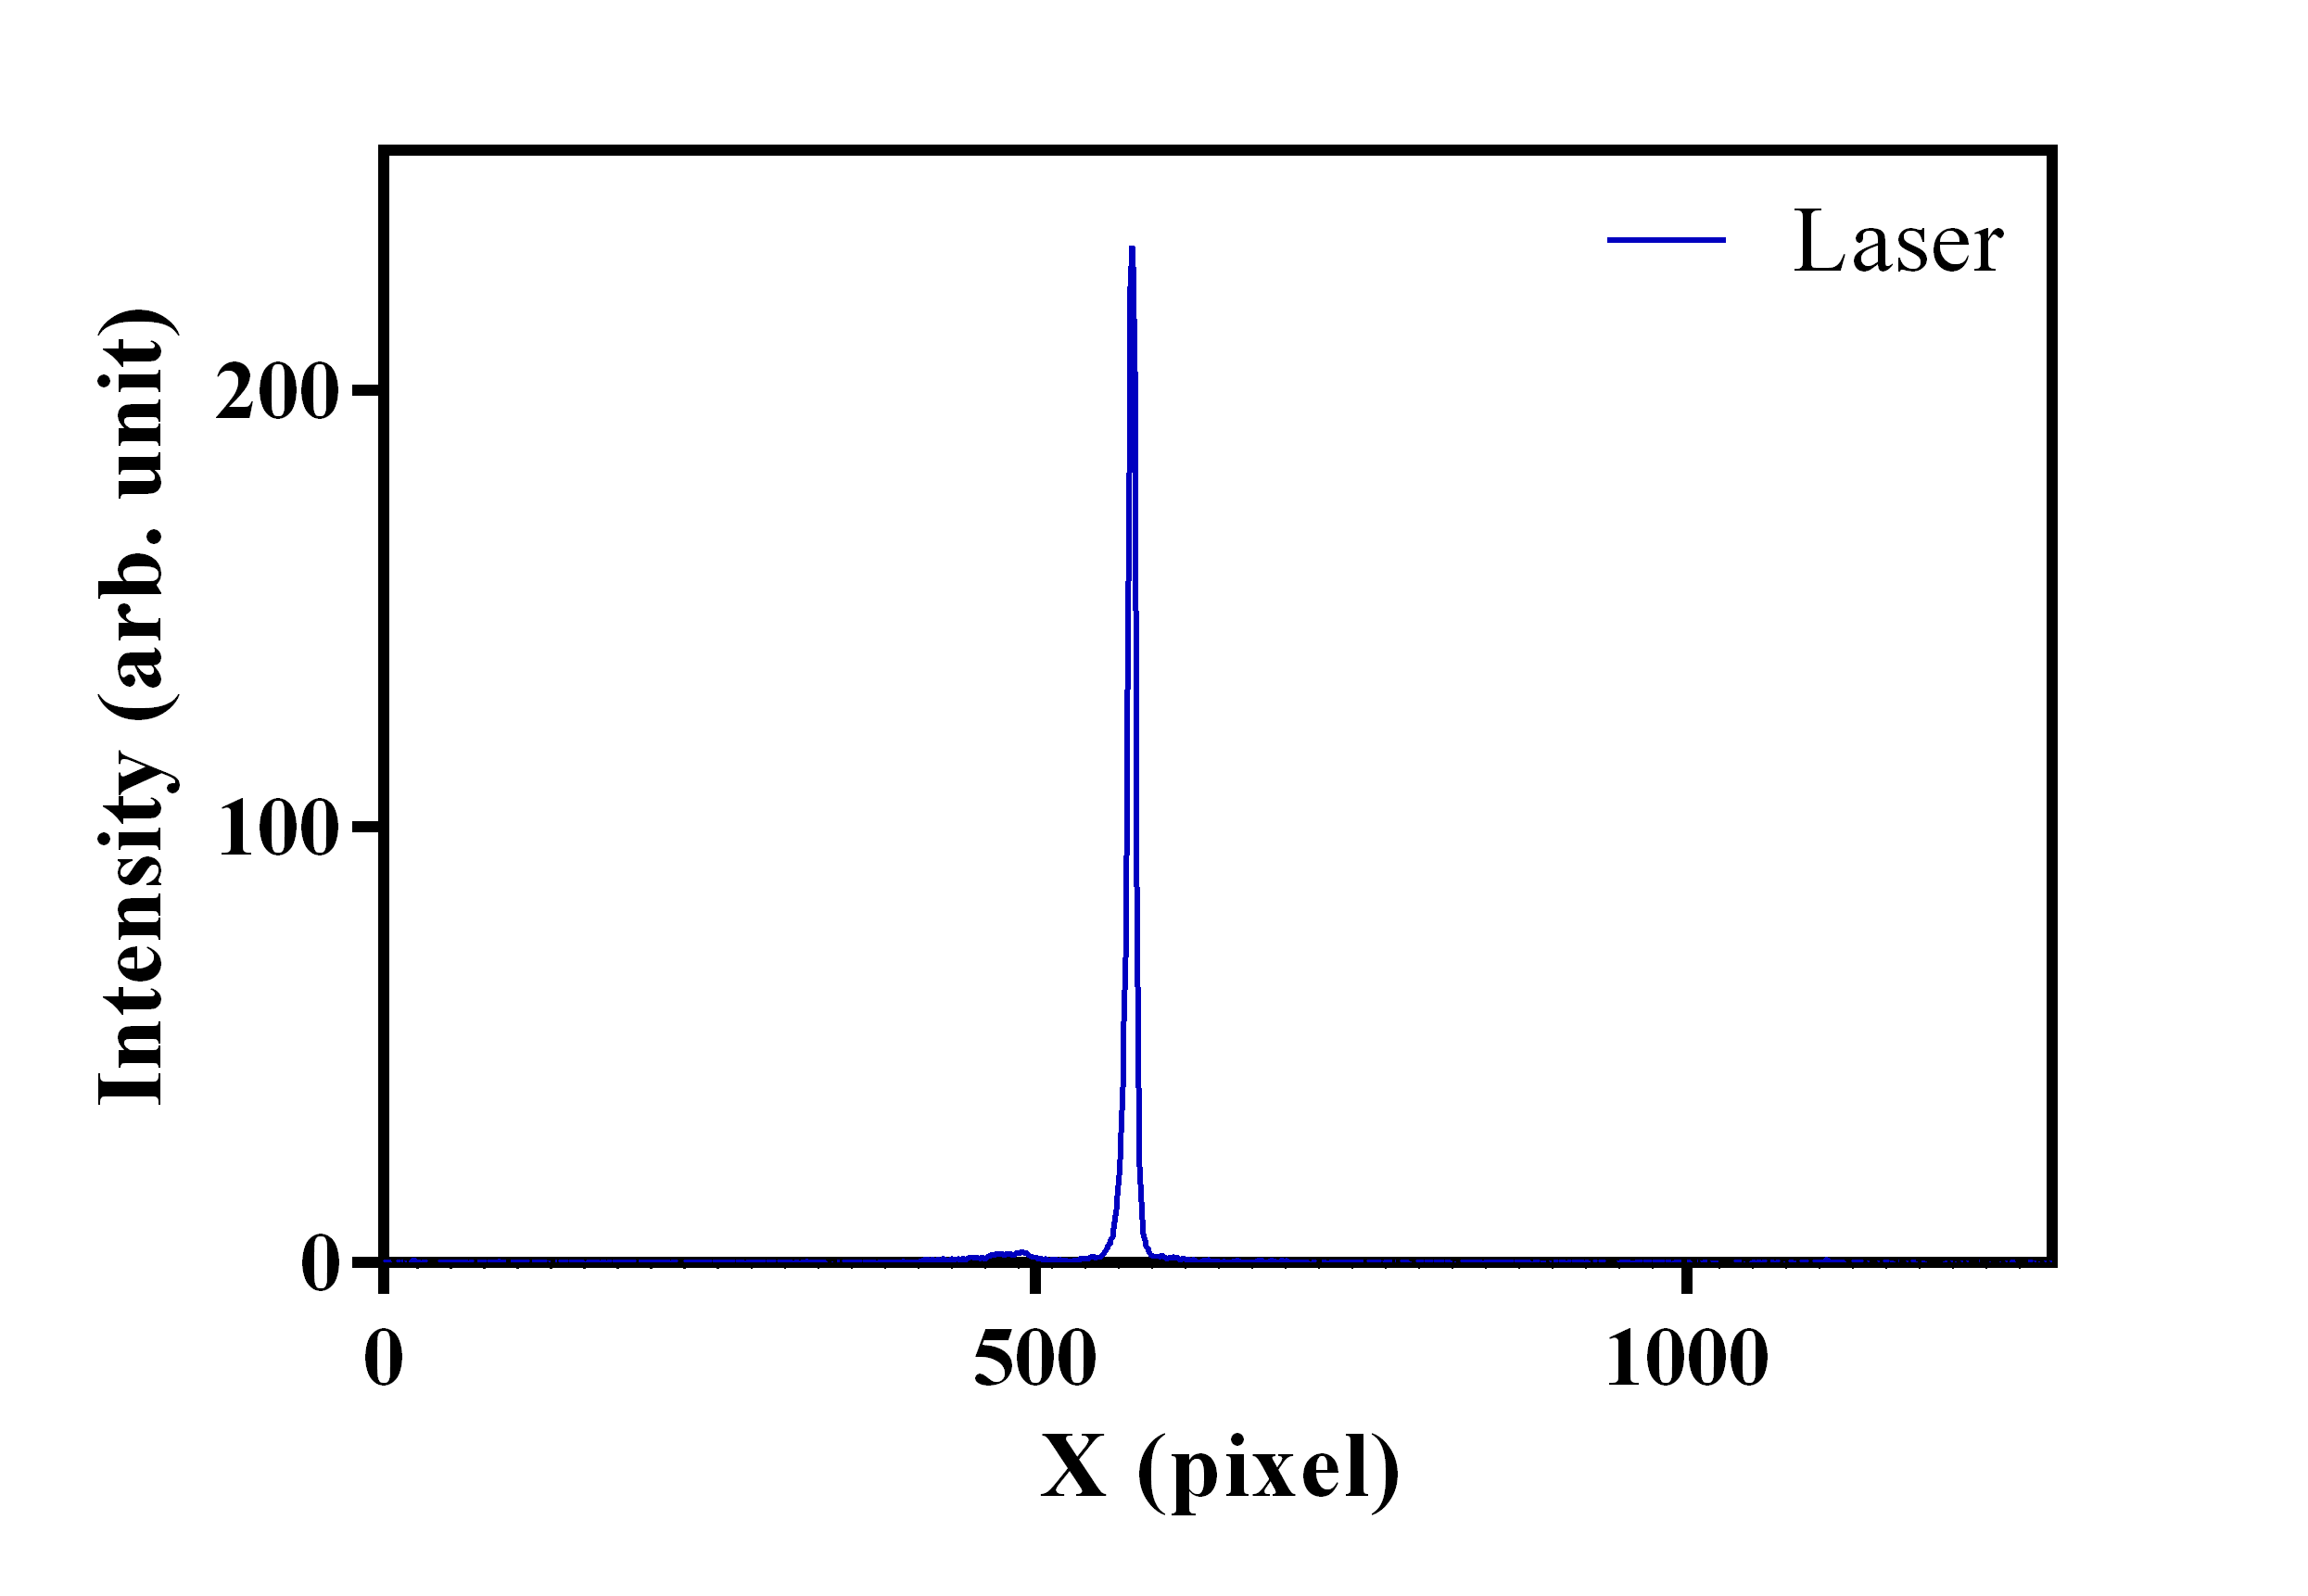
\includegraphics[width=\textwidth]{figures/Laser_raw.png} %插入图片,[]中设置图片大小,{}中是图片文件名
	\caption{雷射光譜強度波型圖} %最终文档中希望显示的图片标题
	\label{雷射光譜強度波型圖} %用于文内引用的标签
\end{figure}
由圖\ref{雷射光譜強度波型圖}. 中可看出此雷射之二階光位置落於影像感測器外,但考量到波長較短的雷射所產生二階光如圖\ref{較短波長的雷射光譜強度波型圖}. 所示,仍會落在影像感測器中,因此在光譜波形套用勞倫茲模型擬合前,仍需對數據進行分區,確保所有分割後區域內僅存在一波峰。
\begin{figure}[H] %H为当前位置,!htb为忽略美学标准,htbp为浮动图形
	\centering %图片居中
	\vspace{0.8cm}
	%\setlength{\abovecaptionskip}{1cm}
	\setlength{\abovecaptionskip}{0.cm}
	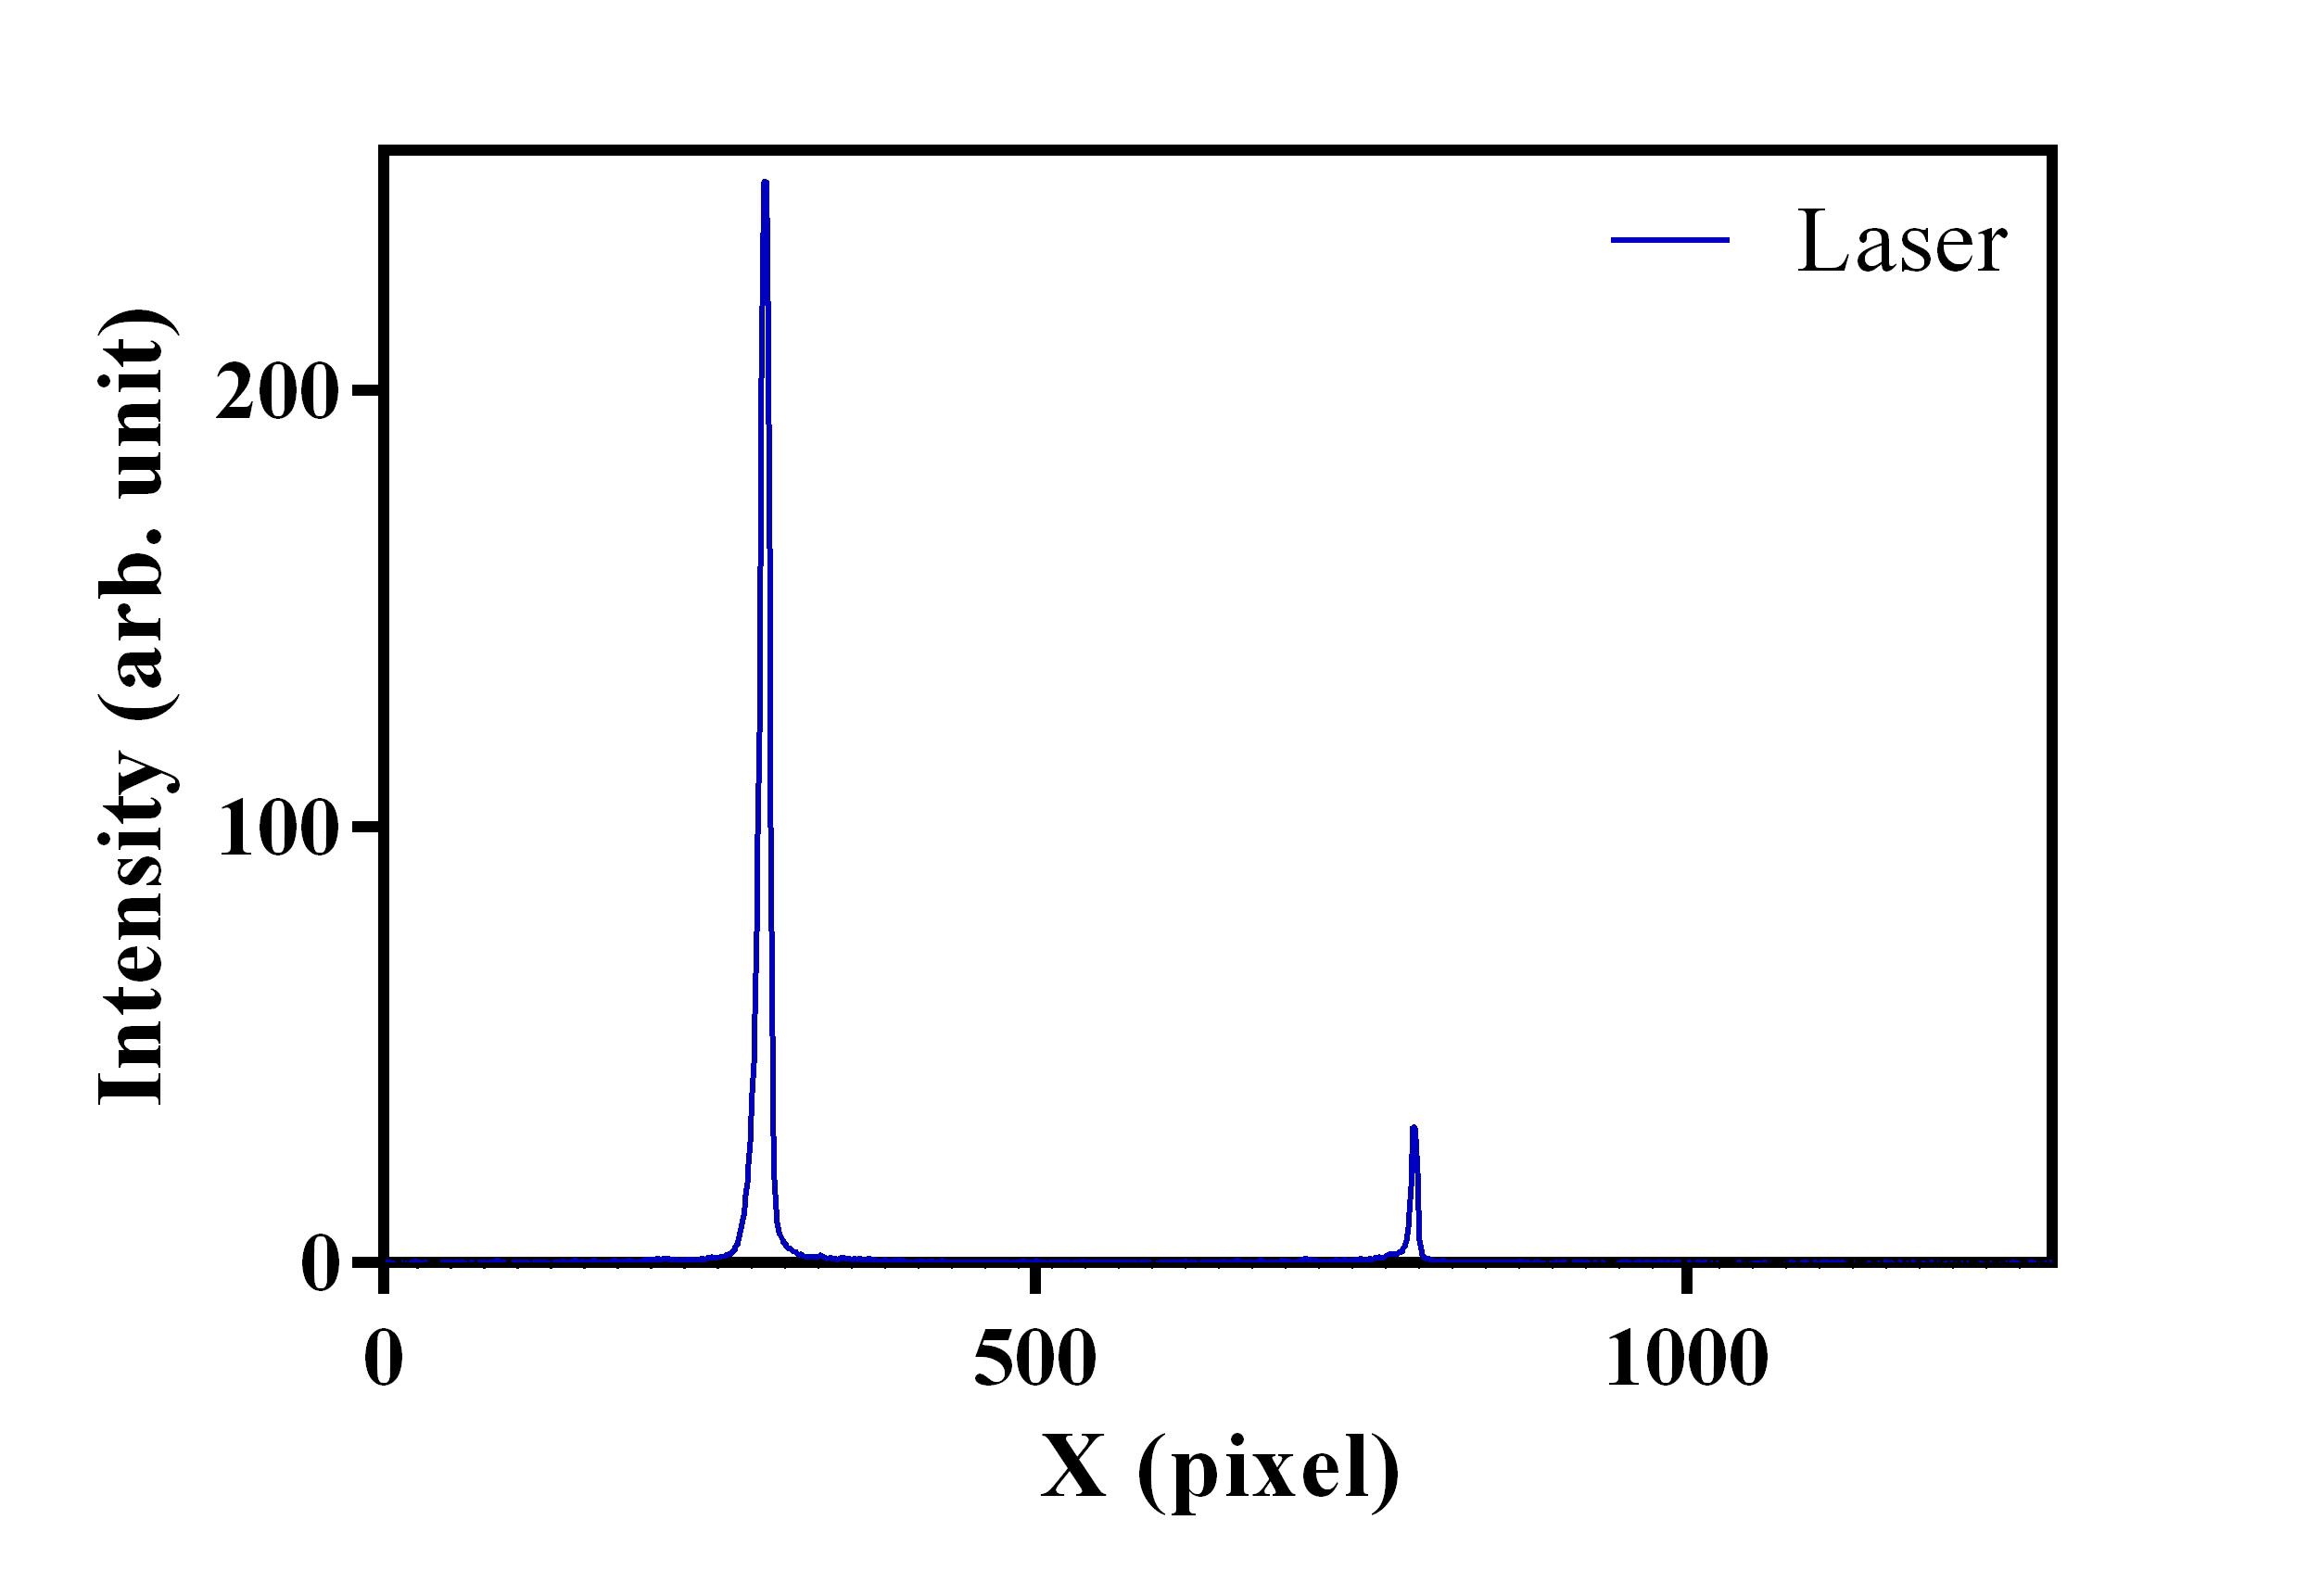
\includegraphics[width=\textwidth]{figures/Laser_1.png} %插入图片,[]中设置图片大小,{}中是图片文件名
	\caption{較短波長的雷射光譜強度波型圖} %最终文档中希望显示的图片标题
	\label{較短波長的雷射光譜強度波型圖} %用于文内引用的标签
\end{figure}
雷射區域分割的判定方法與汞氬燈相同,使用斜率分割出波峰所在區域,再以強度過濾二階光的波峰區域。首先找出所有雷射光譜數據的區域最大與最小值,並將所有點數依像素位置猶大至小排列,如圖\ref{雷射光譜區域最大值與最小值像素位置表示圖}. 所示。波峰所在位置必定為一區域最大值,且此一區域最大值不同於其餘區域最大值,斜率必將夾於一正斜率線段與負斜率線段中,且此一斜率絕對值將遠高於其餘線段斜率,因此透過兩點間斜率判定與斜率正負夾擠法,便可以過濾出如圖\ref{雷射光譜以斜率分割後之波峰區域表示圖}. 所示四點區分出兩個峰值所在區域。
\begin{figure}[H] %H为当前位置,!htb为忽略美学标准,htbp为浮动图形
	\centering %图片居中
	%\setlength{\abovecaptionskip}{1cm}
	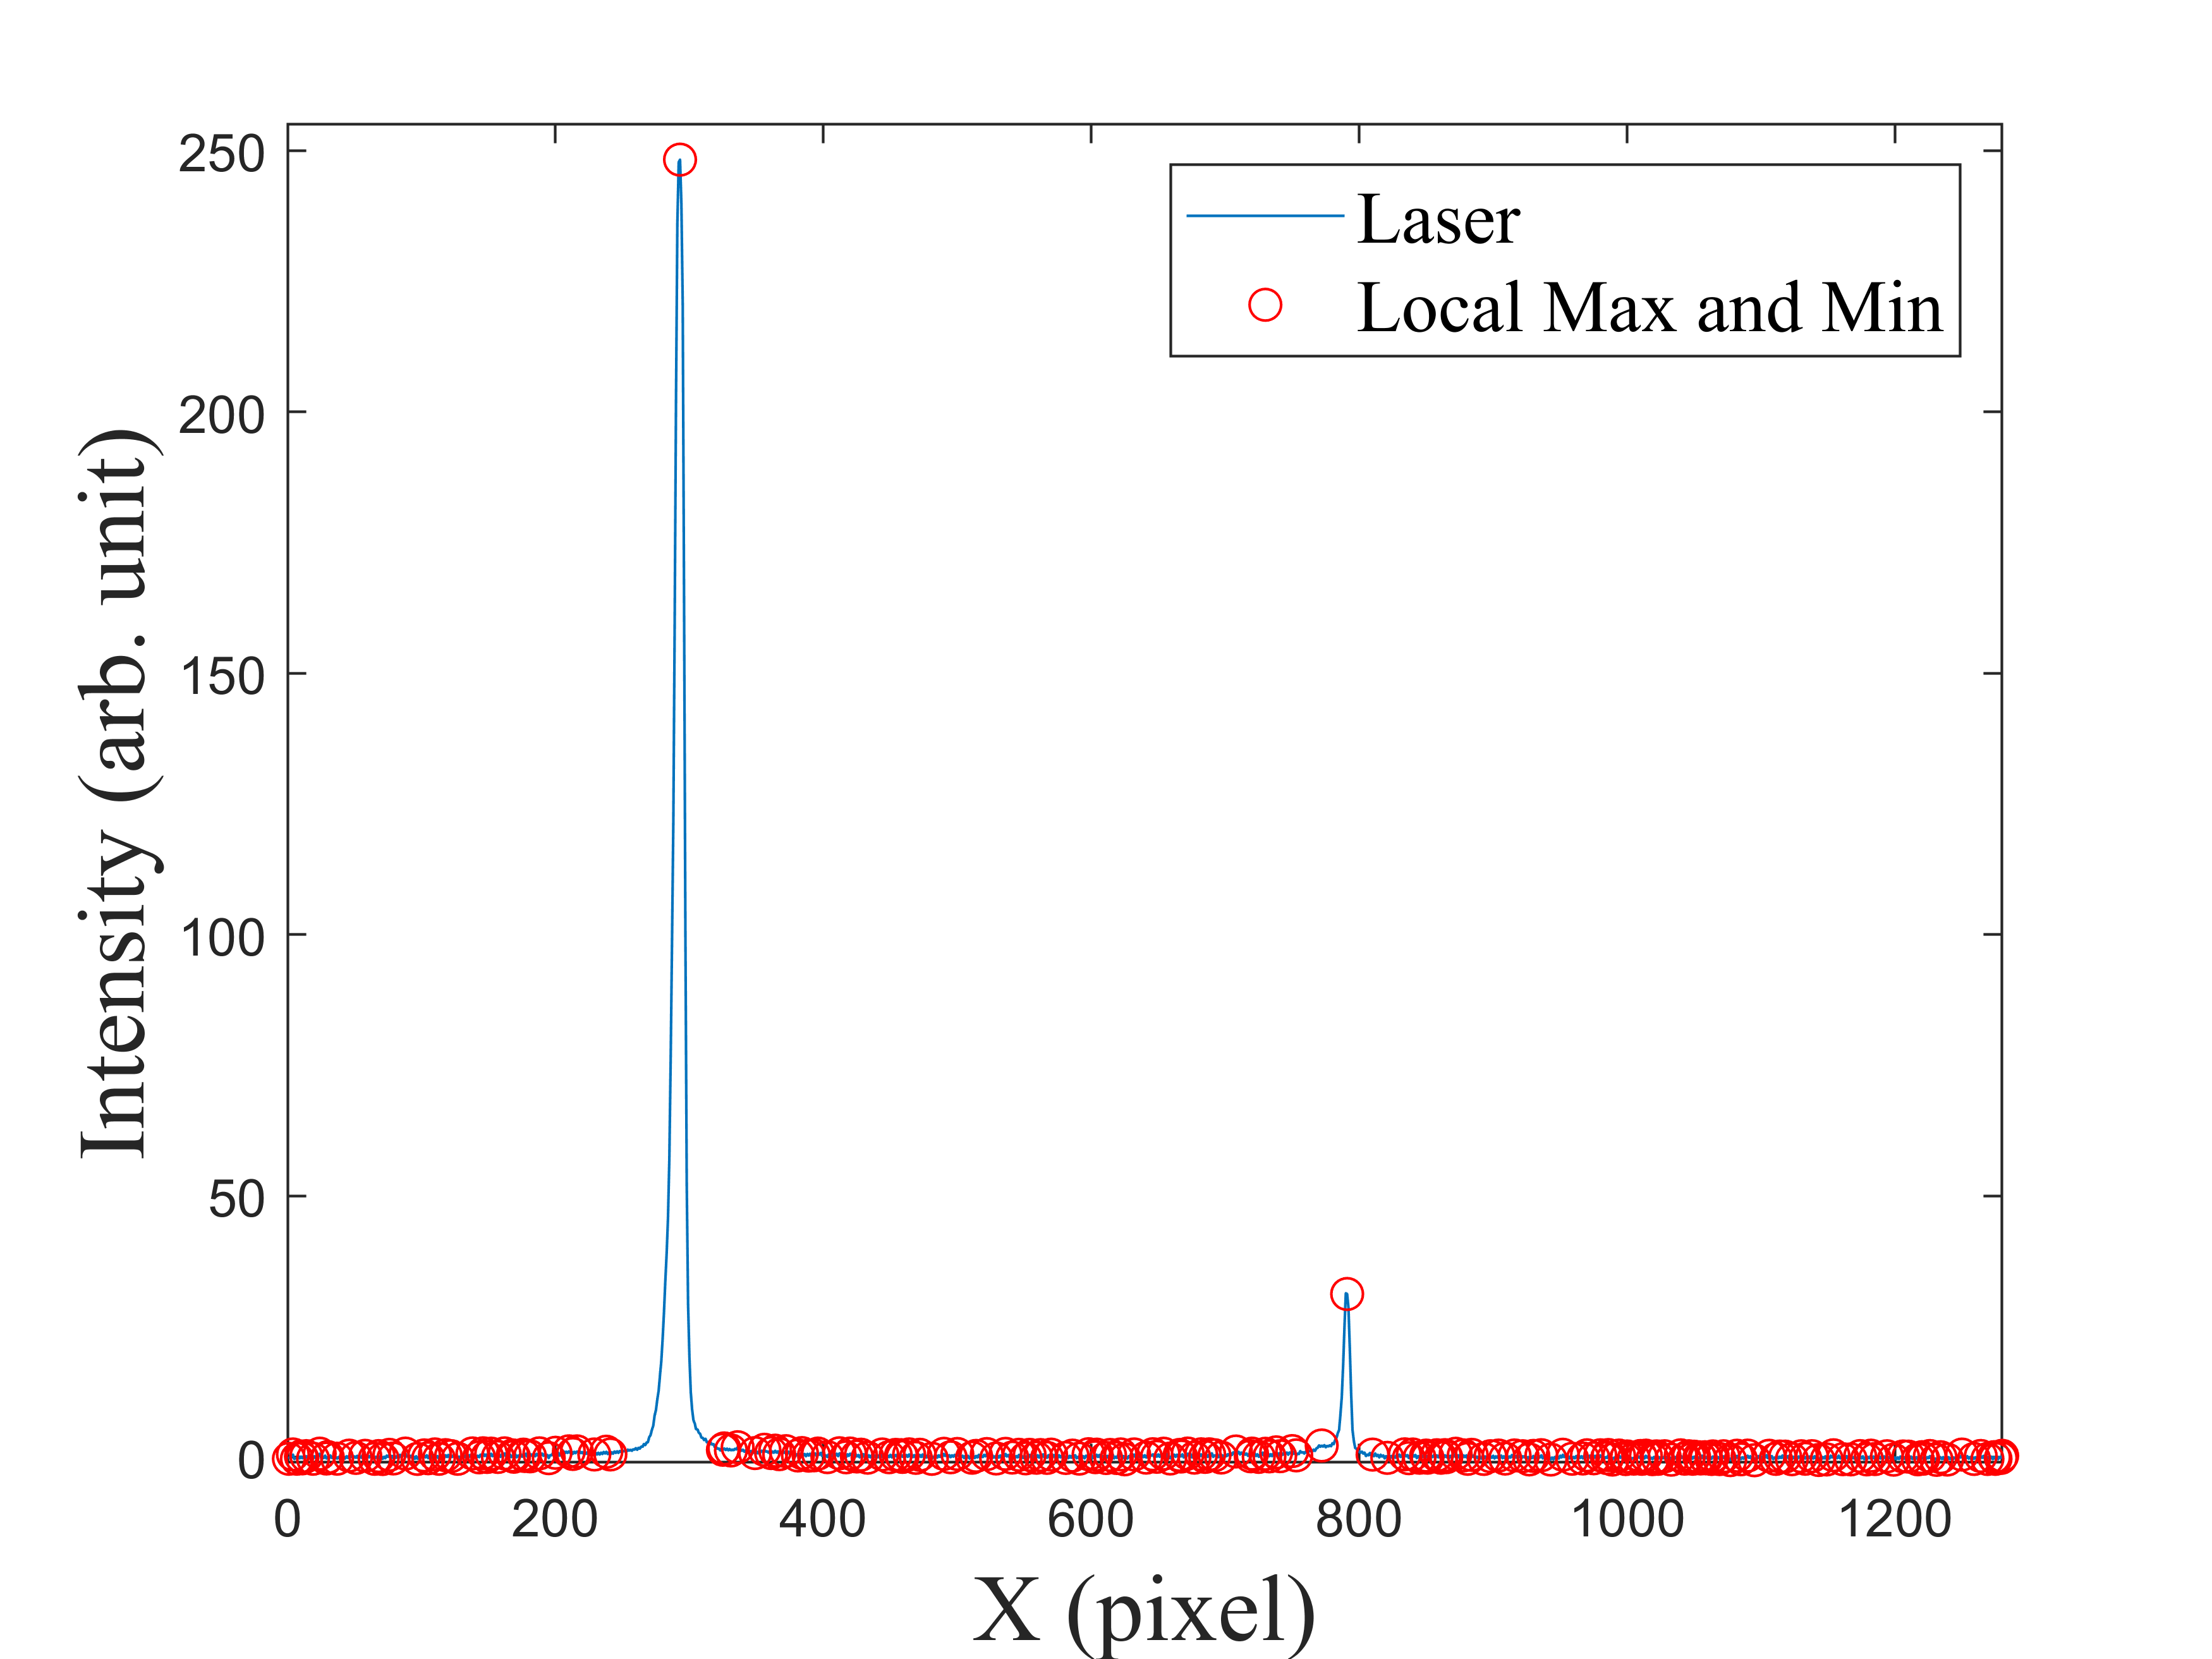
\includegraphics[width=14.5cm]{figures/LASER_MIN_MAX.png} %插入图片,[]中设置图片大小,{}中是图片文件名
	\caption{雷射光譜區域最大值與最小值像素位置表示圖} %最终文档中希望显示的图片标题
	\label{雷射光譜區域最大值與最小值像素位置表示圖} %用于文内引用的标签
\end{figure}

\begin{figure}[H] %H为当前位置,!htb为忽略美学标准,htbp为浮动图形
	\centering %图片居中
	%\setlength{\abovecaptionskip}{1cm}
	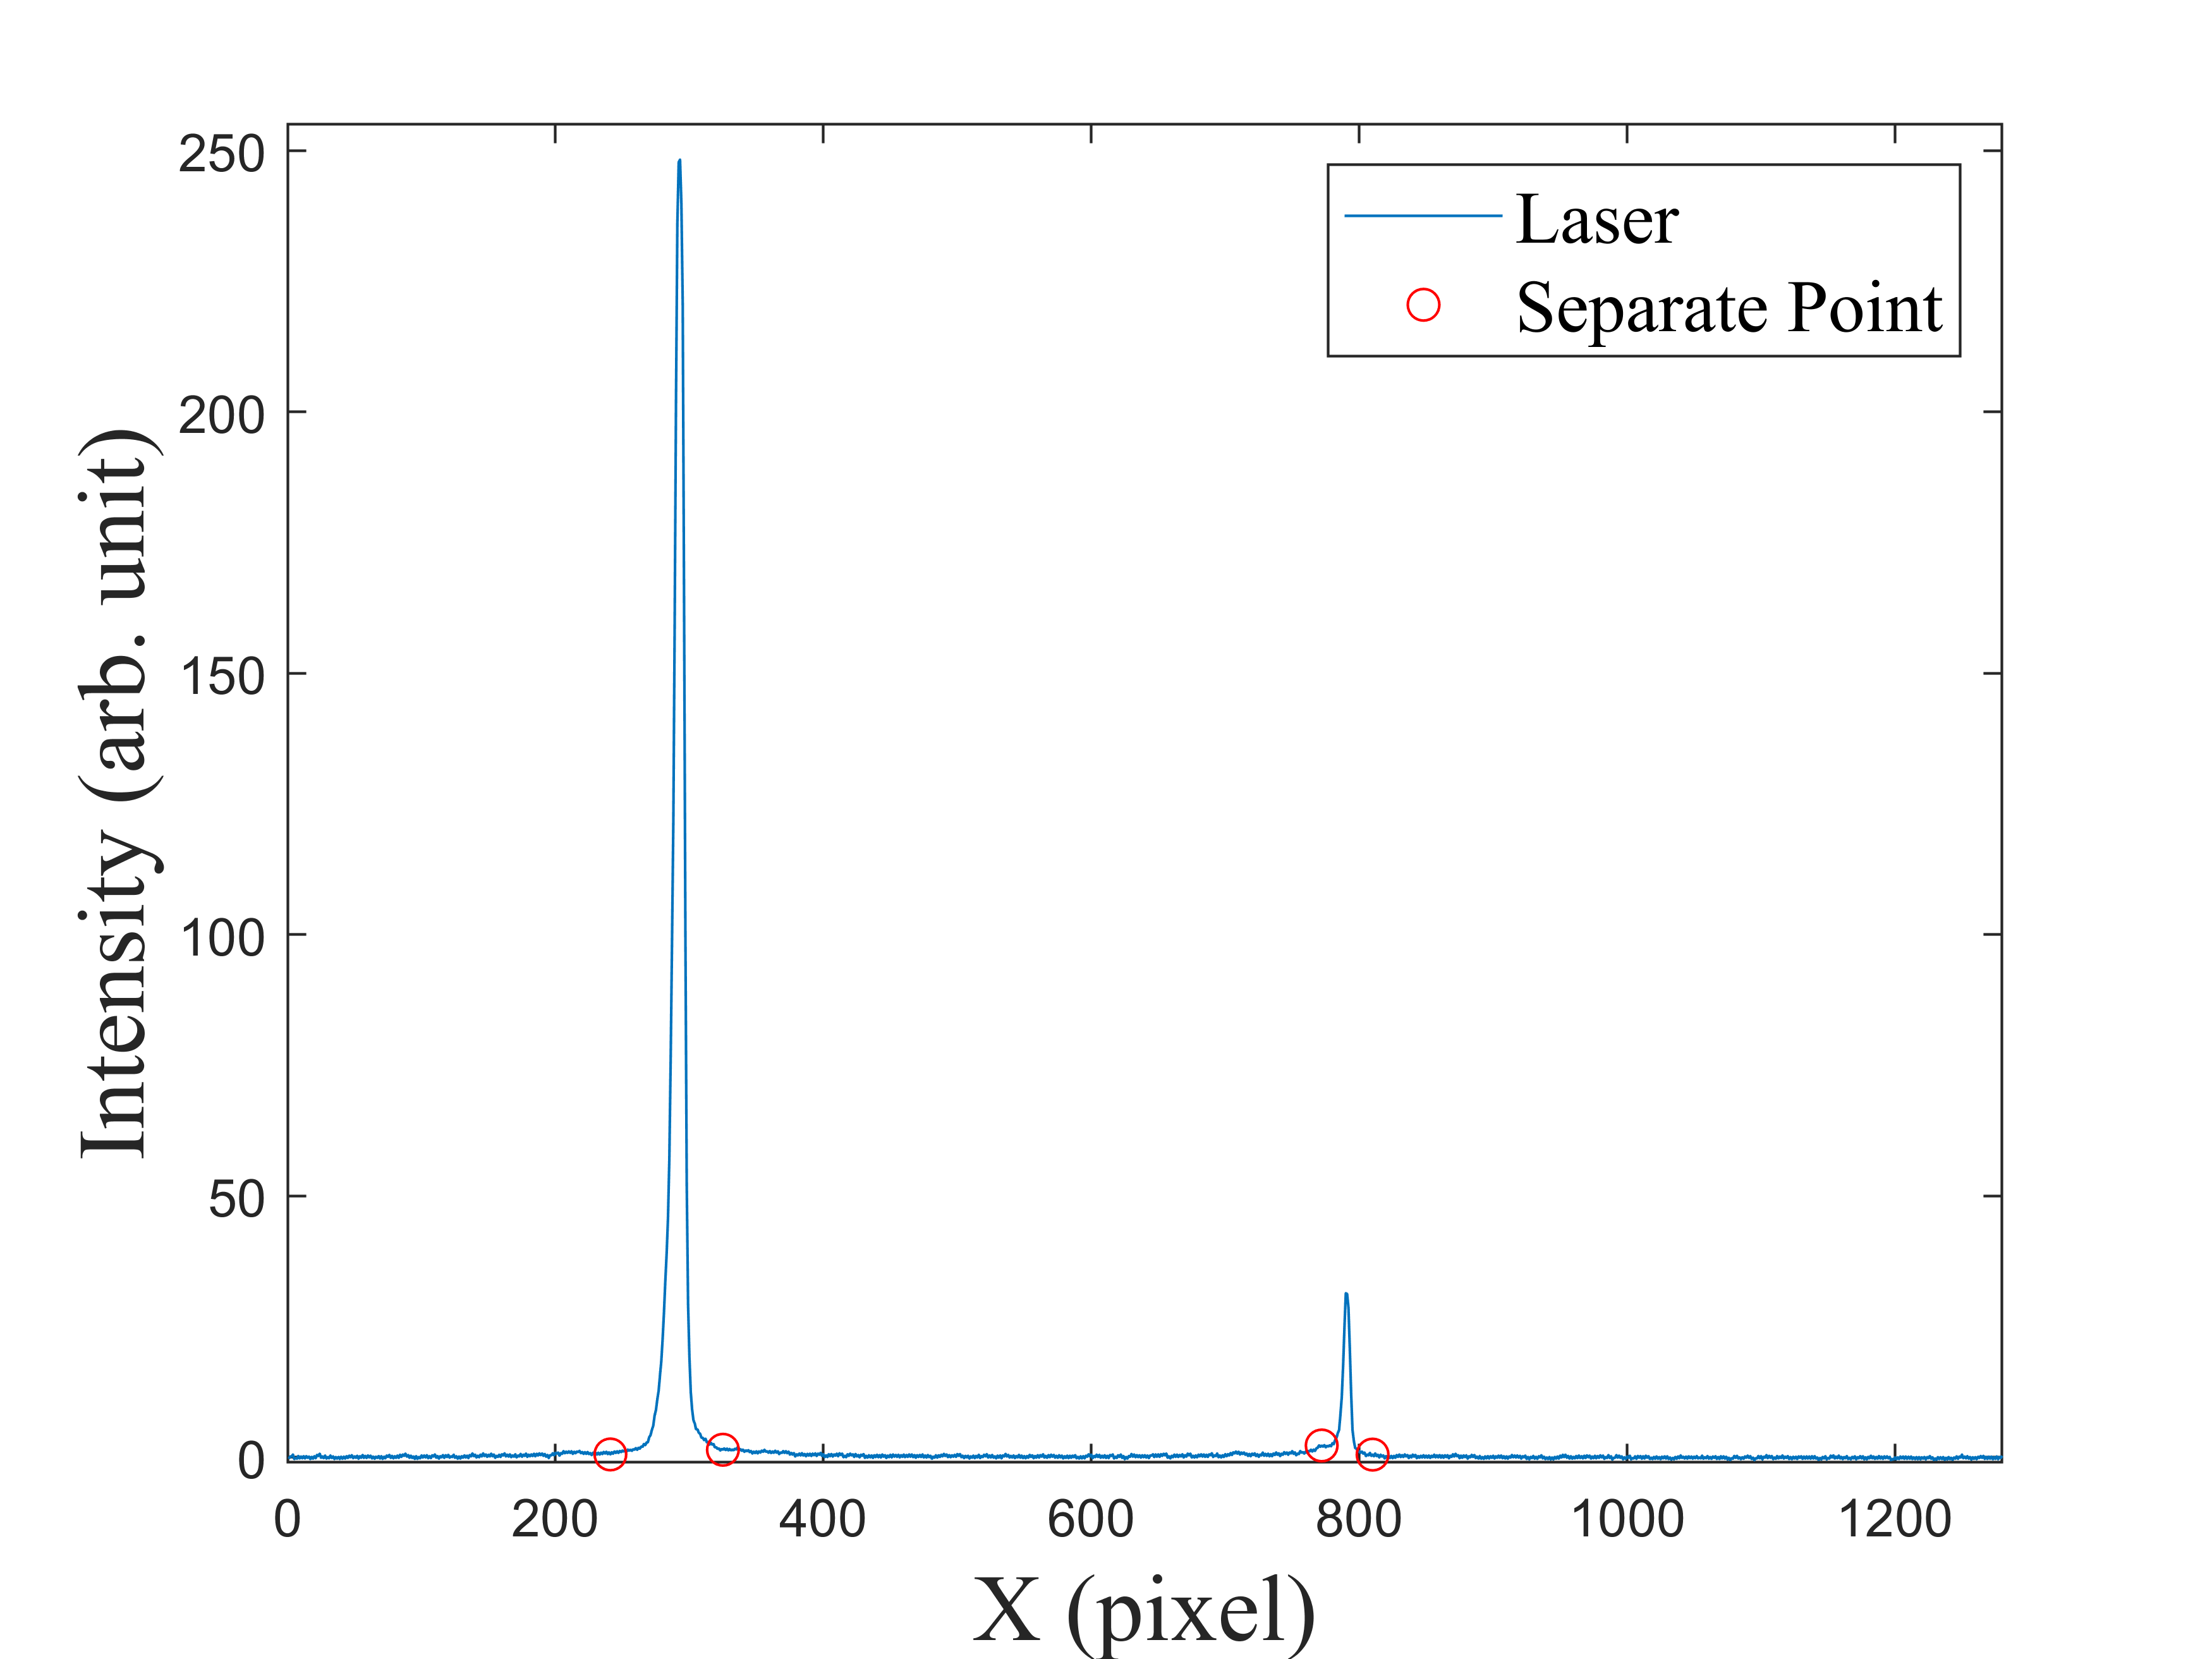
\includegraphics[width=14.5cm]{figures/LASER_SEP.png} %插入图片,[]中设置图片大小,{}中是图片文件名
	\caption{雷射光譜以斜率分割後之波峰區域表示圖} %最终文档中希望显示的图片标题
	\label{雷射光譜以斜率分割後之波峰區域表示圖} %用于文内引用的标签
\end{figure}
由圖\ref{雷射光譜以斜率分割後之波峰區域表示圖}. 中可以明顯看出,當在波長較低之雷射進行區域分割後,由於存在雷射的二階光的影響,因此數據分割後的波峰區域仍包含二階光波峰所在區域,為了要找出主要波峰的數據區域,僅需透過區域最大值的強度與其所在的位置,則可以輕易判斷出主要雷射波峰所在的區域,保留主要波峰區域並且剃除二階光產生的波峰的區域後,最後的分區結果如圖\ref{雷射光譜以強度過濾後之主波峰區域表示圖}. 所示。
\begin{figure}[H] %H为当前位置,!htb为忽略美学标准,htbp为浮动图形
	\centering %图片居中
	\vspace{0.8cm}
	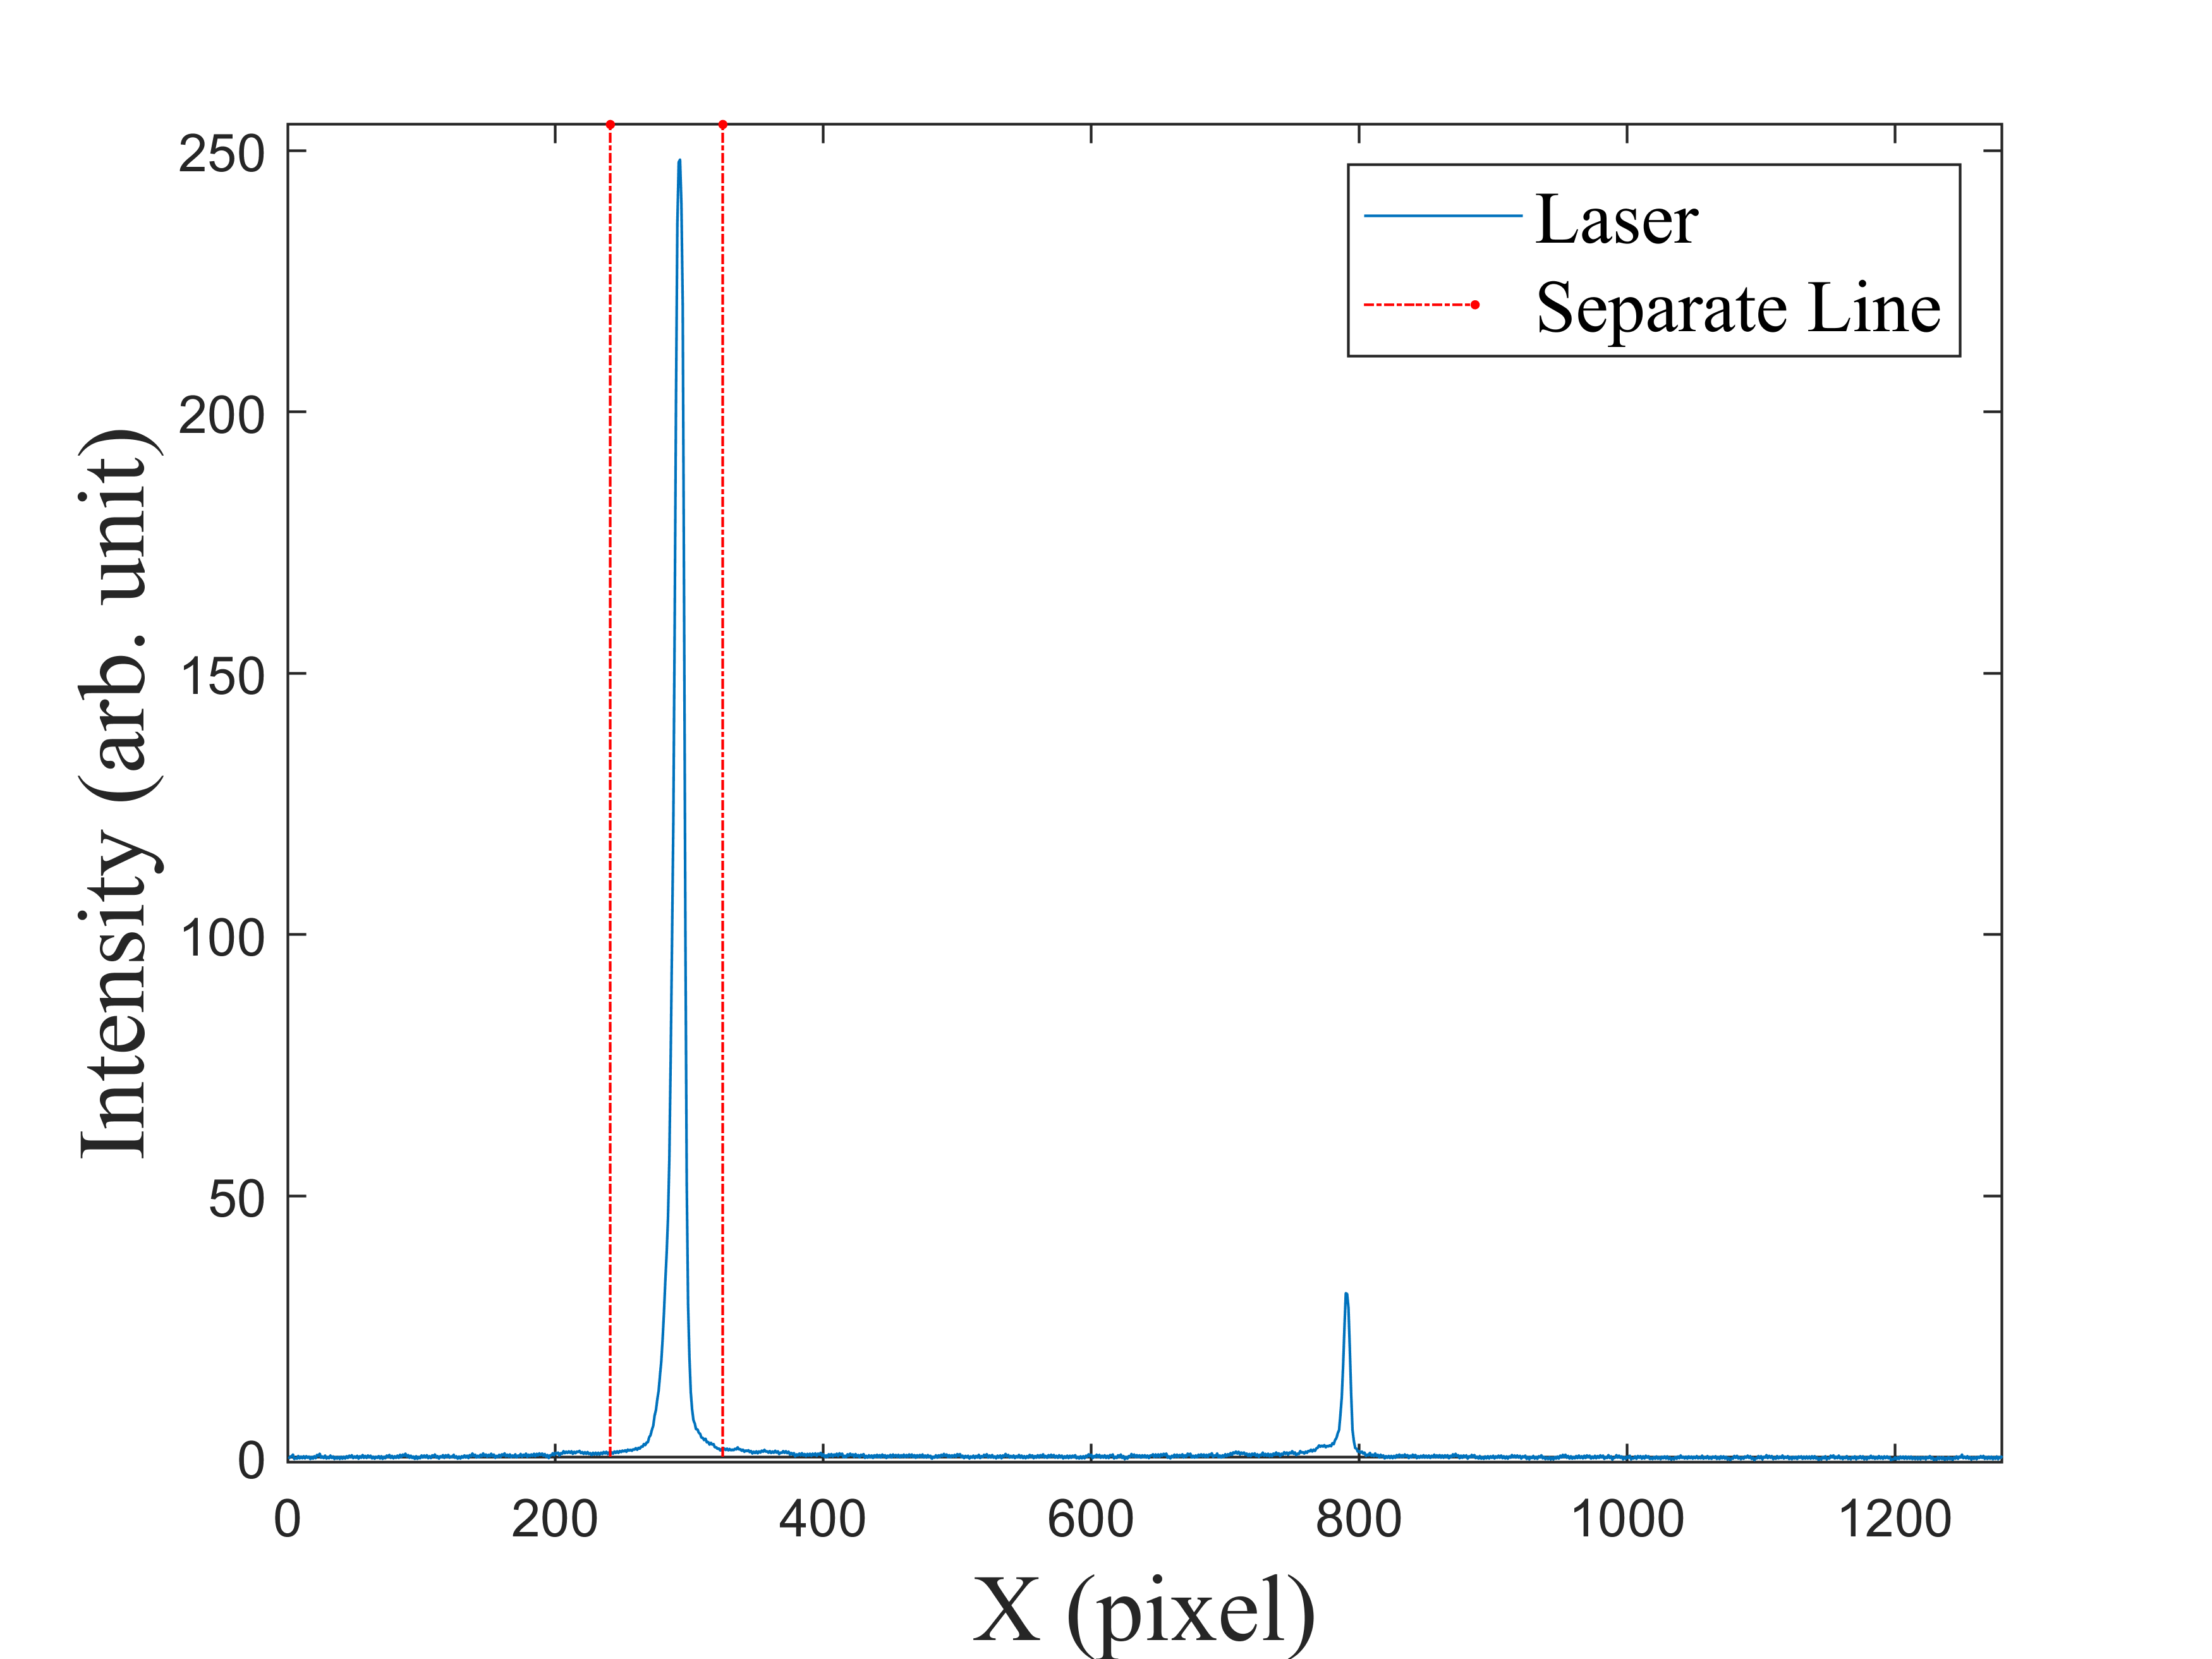
\includegraphics[width=16cm]{figures/laser_sep_only1area.png} %插入图片,[]中设置图片大小,{}中是图片文件名
	\caption{雷射光譜以強度過濾後之主波峰區域表示圖} %最终文档中希望显示的图片标题
	\label{雷射光譜以強度過濾後之主波峰區域表示圖} %用于文内引用的标签
\end{figure}
\newpage
如第二章表\ref{光源介紹表}. 所述,雷射光束的光譜波形最適合以勞倫茲模型函數擬合,因此將雷射主波峰所在區域波形數據以勞倫茲模型擬合後,便可得出雷射精確的波峰位置、半高全寬與波峰強度,擬合結果如圖\ref{雷射光譜主波峰區域進行勞倫茲擬合後結果圖}. 所示。
\begin{figure}[H] %H为当前位置,!htb为忽略美学标准,htbp为浮动图形
	\centering %图片居中
	\vspace{0.8cm}
	\setlength{\abovecaptionskip}{0.cm}
	%\setlength{\abovecaptionskip}{1cm}
	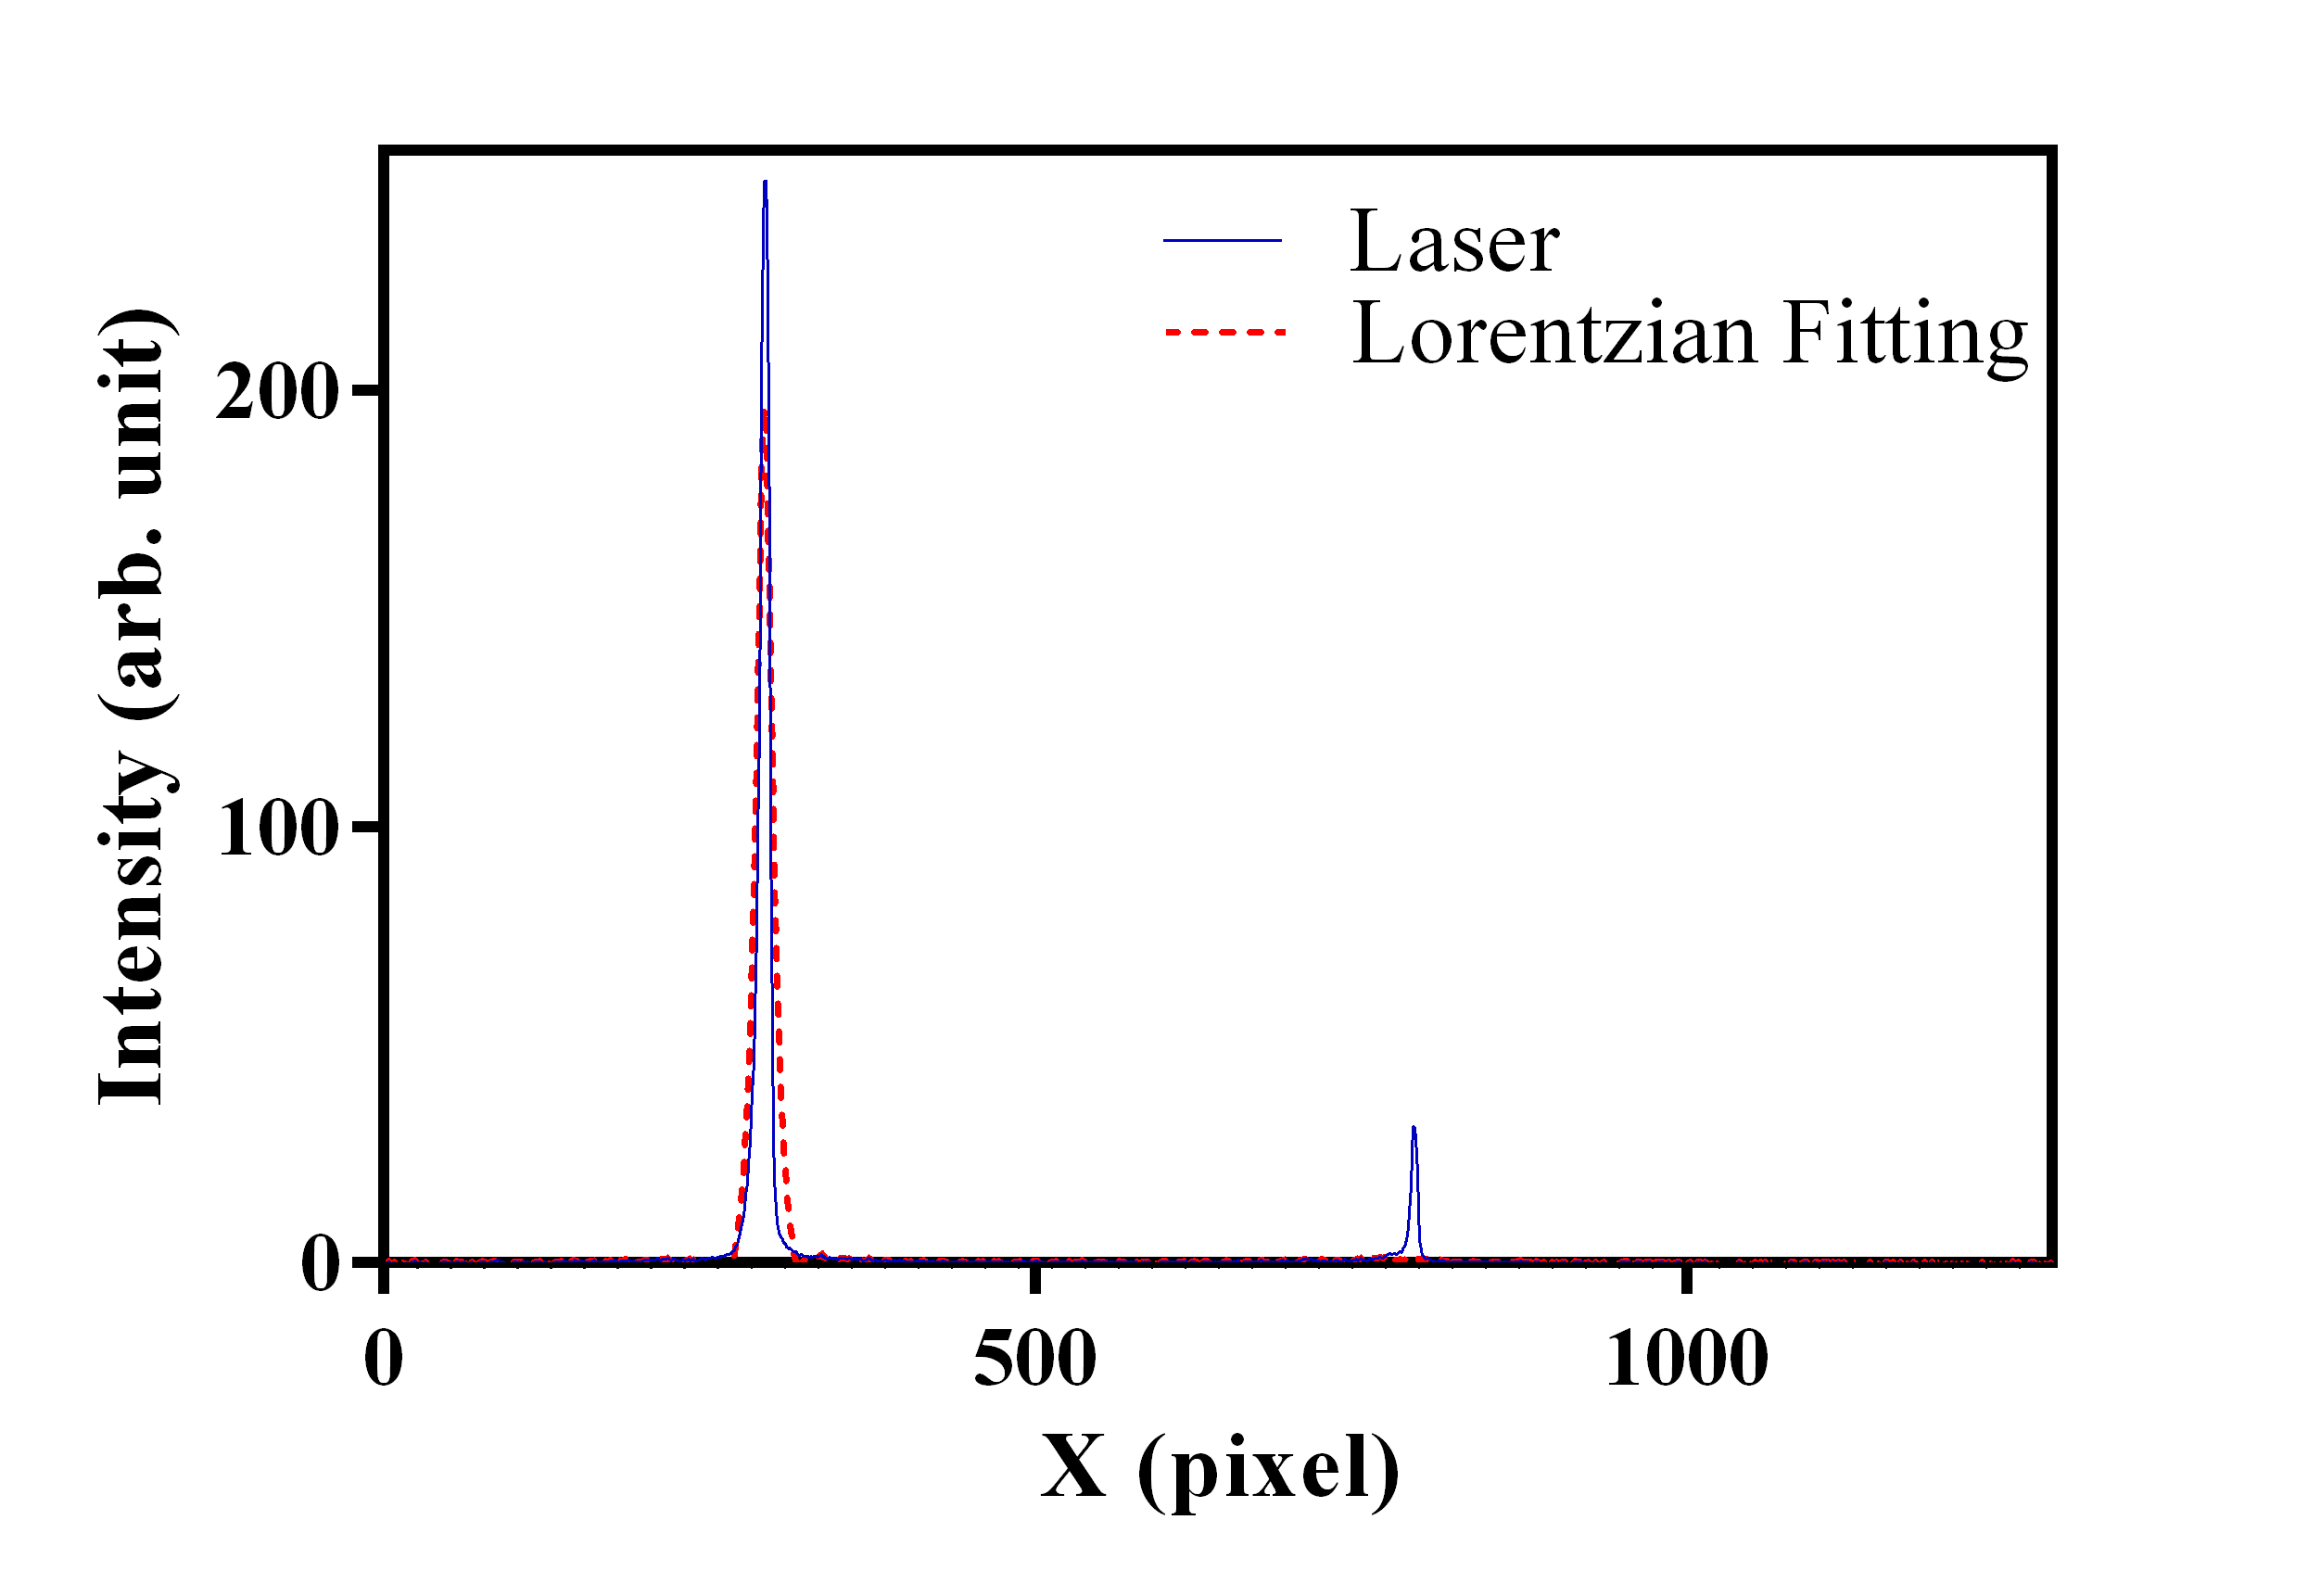
\includegraphics[width=\textwidth]{figures/L1_Lorentz.png} %插入图片,[]中设置图片大小,{}中是图片文件名
	\caption{雷射光譜主波峰區域進行勞倫茲擬合後結果圖} %最终文档中希望显示的图片标题
	\label{雷射光譜主波峰區域進行勞倫茲擬合後結果圖} %用于文内引用的标签
\end{figure}
將擬合後得出的波峰位置記憶於程式站存記憶體中,並依序個別對不同波長之雷射光源重複進行單雷射波峰位置偵測,直至取得所有雷射光源的準確波峰位置,所有雷射波峰偵測結果疊圖如圖\ref{所有單雷射光譜經單雷射波峰位置偵測後結果疊圖}. 所示,而所有雷射光譜由勞倫茲擬合後取得之準確波峰所在像素位置如表\ref{所有單雷射波峰經波峰偵測後所得出之參數表}. 所示。
\begin{figure}[H] %H为当前位置,!htb为忽略美学标准,htbp为浮动图形
	\centering %图片居中
	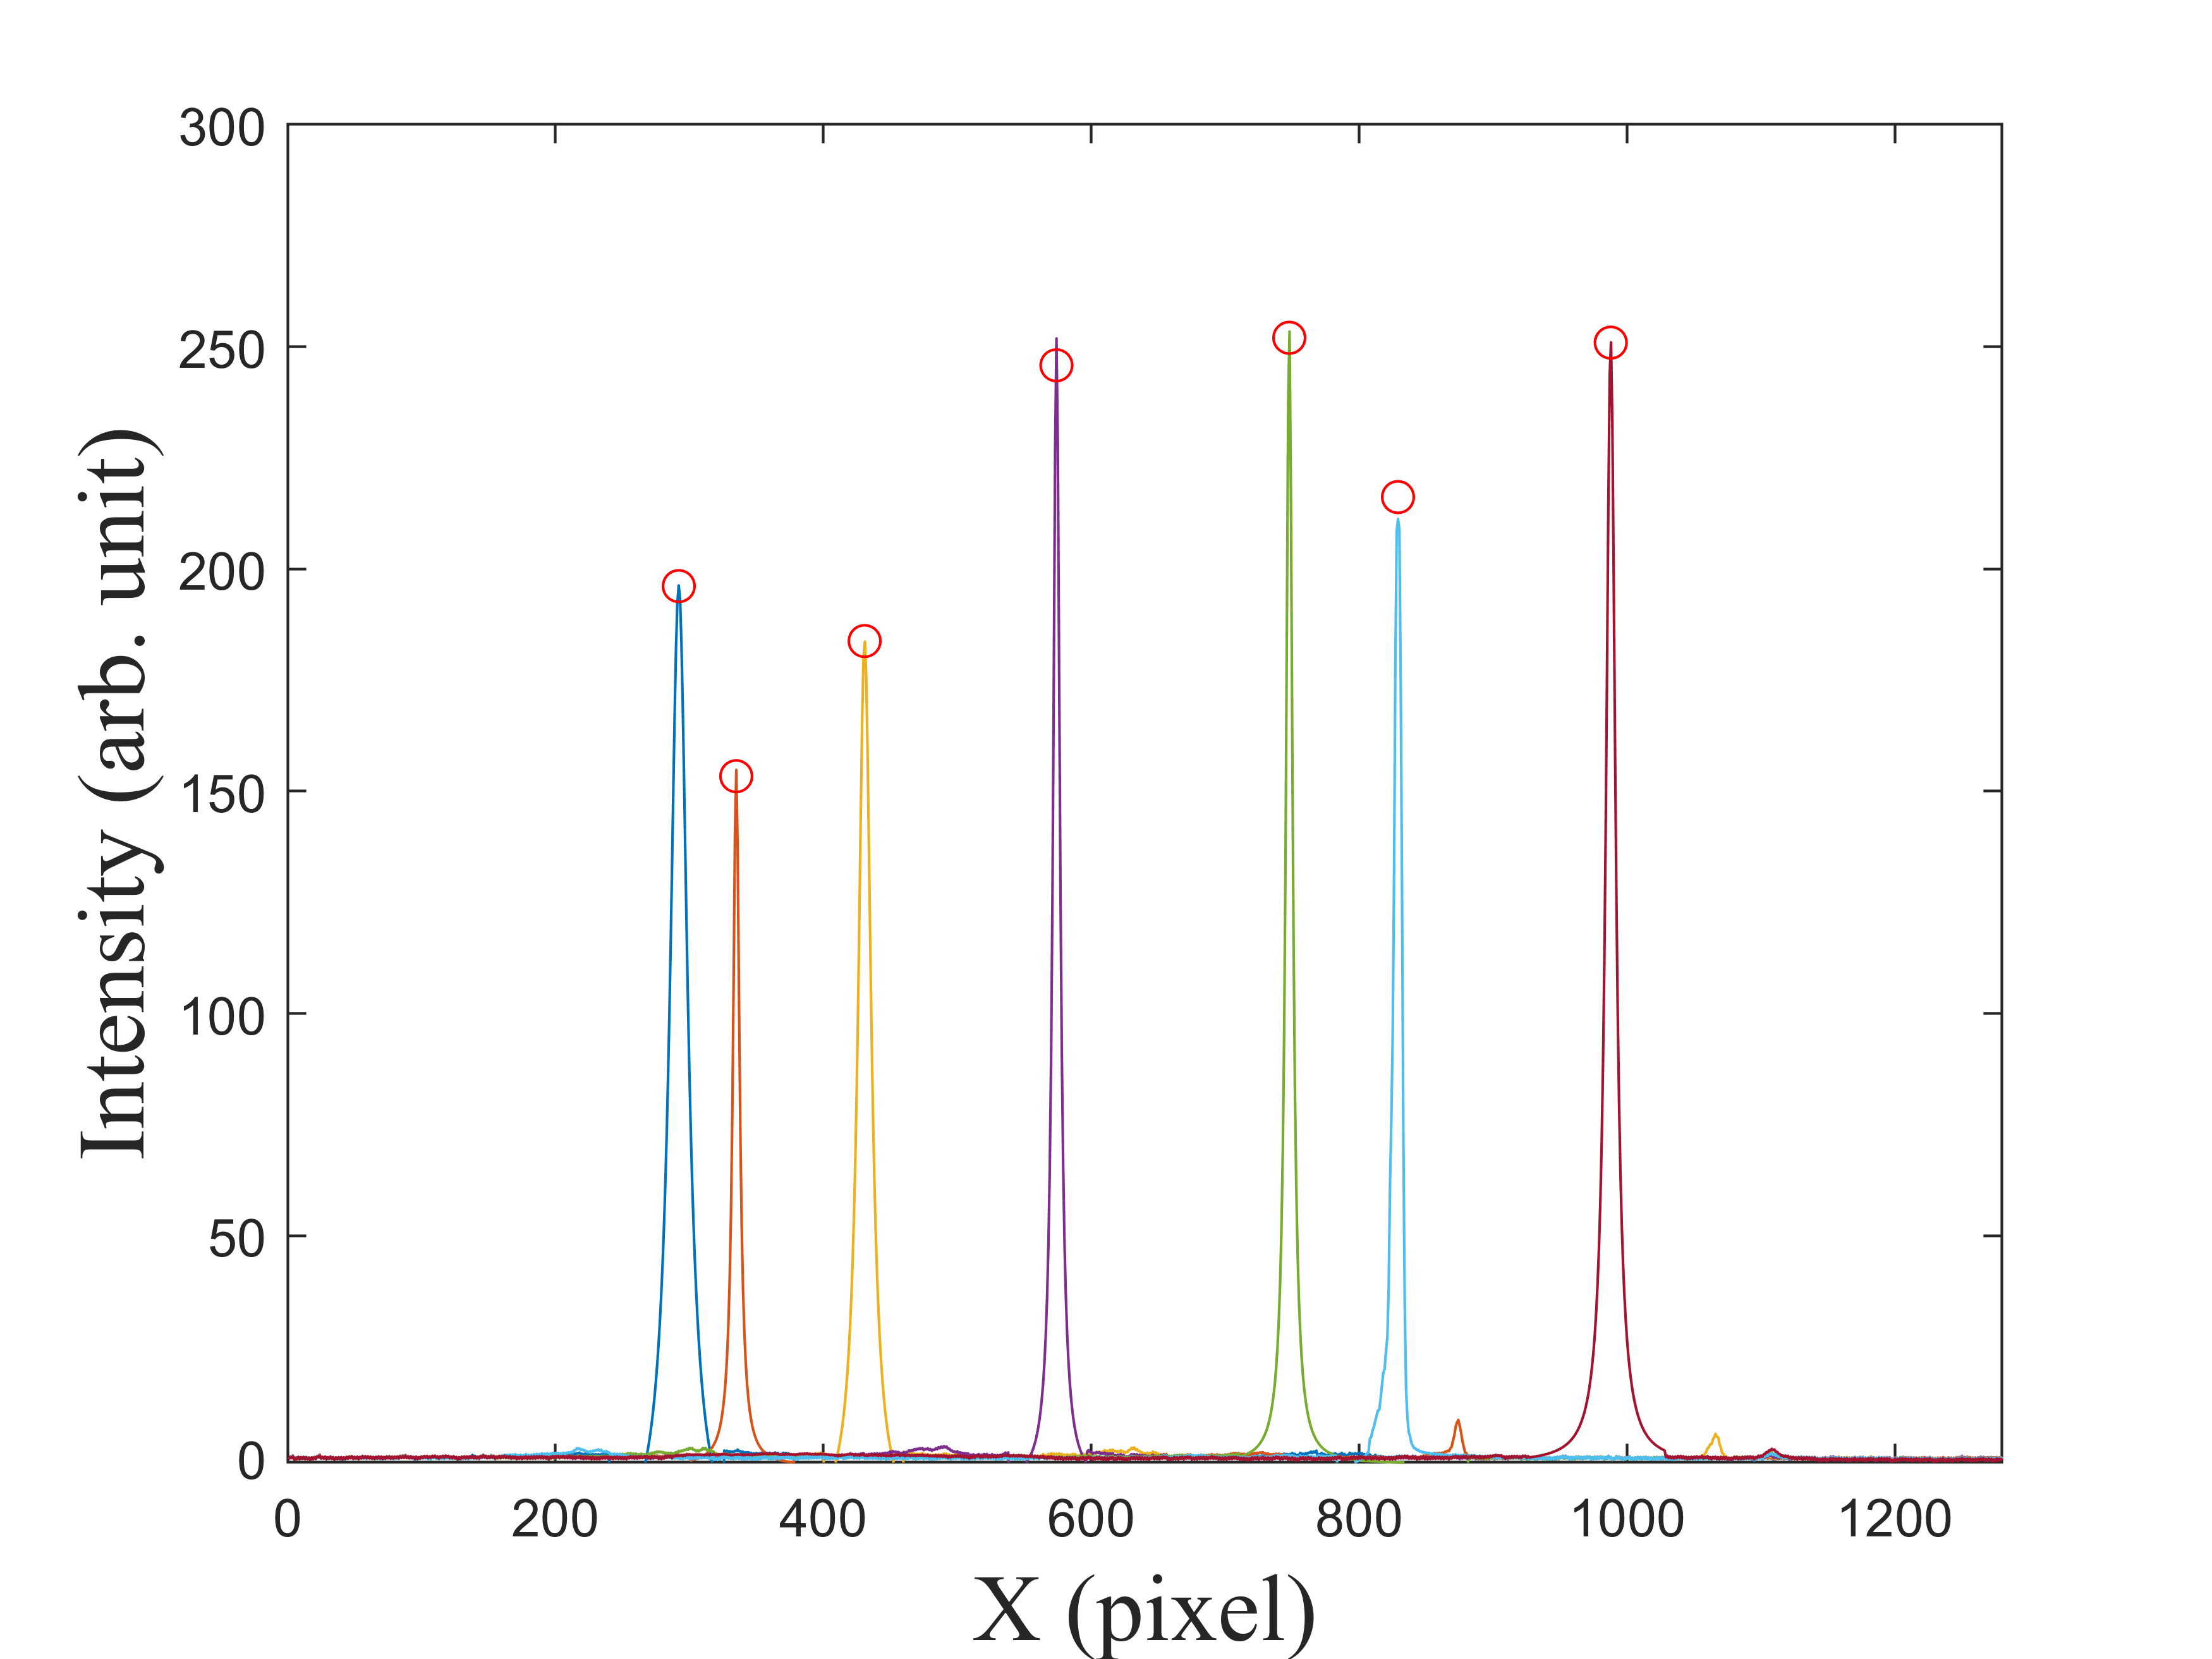
\includegraphics[width=16cm]{figures/AllLaserPeak.png} %插入图片,[]中设置图片大小,{}中是图片文件名
	\caption{所有單雷射光譜經單雷射波峰位置偵測後結果疊圖} %最终文档中希望显示的图片标题
	\label{所有單雷射光譜經單雷射波峰位置偵測後結果疊圖} %用于文内引用的标签
\end{figure}
\begin{center}
	\vspace{0.8cm}
	\captionof{table}{所有單雷射波峰經波峰偵測後所得出之參數表}\label{所有單雷射波峰經波峰偵測後所得出之參數表}
\begin{tabularx}{\textwidth}{m{0.2\textwidth}<{\centering}c m{0.25\textwidth}<{\centering}c}
	\hline\hline
	光源&峰值位置(pixel) & 強度 & 半高全寬(pixel)\\		
	\hline
	雷射1&292.0486	&196.1531&	12.8644\\
	雷射2&334.9441	&153.3864&	5.4504\\
	雷射3&430.7891	&183.7902&	9.5892\\
	雷射5&573.9681	&245.8263&	6.1762\\
	雷射6&747.8033	&252.0191&	5.5141\\
	雷射7&828.9508	&216.1823&	7.4330\\
	雷射8&987.7875	&250.9284&	7.5354\\
	\hline\hline
\end{tabularx}
\end{center}
\section{結合校正}
為了找出晶片空間轉換方程式,需要求出所有波峰的像素與其對應波長才能進行多項式擬合,而在透過一次次的波峰偵測後,現在已獲得所有汞氬燈與雷射目標波峰之準確的峰值所在像素位置,並且已知所有目標波峰與其對應的標準波長,將目標波峰像素位置與其對應標準波長表示於表\ref{所有目標波峰之峰值像素位置與標準波長對應表}. 中。
\begin{center}
	\vspace{0.8cm}
\captionof{table}{所有目標波峰之峰值像素位置與標準波長對應表}\label{所有目標波峰之峰值像素位置與標準波長對應表}
\begin{tabularx}{\textwidth}{m{0.3\textwidth}<{\centering}m{0.3\textwidth}<{\centering}m{0.3\textwidth}<{\centering}}
	\hline\hline
	光源&峰值位置(pixel) & 標準波長 (nm)\\		
	\hline
	\multirow{4}{*}{汞燈 }
	&287.9697&	404.65\\
	&326.3158&	435.83\\
	&461.6027&	546.07\\
	&500.5412&	578.01\\
	\hline
	\multirow{2}{*}{氬燈 }
	&724.7514&	763.51\\
	&781.2286&	811.53\\  
	\hline	
	雷射1&292.0486	&404.97 \\
	雷射2&334.9441	&443.93 \\
	雷射3&430.7891	&520.69 \\
	雷射5&573.9681	&642.13 \\
	雷射6&747.8033	&784.46 \\
	雷射7&828.9508	&851.04 \\
	雷射8&987.7875	&981.67 \\
	\hline\hline
\end{tabularx}
\vspace{10pt}
\end{center}
將表\ref{所有目標波峰之峰值像素位置與標準波長對應表}. 中所有汞氬燈與雷射目標波峰之峰值像素位置以變數$P$表示,而與其對應之標準波長則以變數$\lambda$表示,將每一組對應變數結合成一組數據$(P_i,\lambda_i)$,則波長空間與像素空間之三次轉換公式為
\begin{equation}\label{eq3.3}
	\lambda_i= a_0+a_1 P_i+a_2 P_{i}^2+a_3 P_{i}^3
\end{equation}
將所有數據組帶入方程式(\ref{eq3.3})並以矩陣表示為
\begin{equation}\label{eq3.4}
	\begin{bmatrix} \lambda_1\\\lambda_2\\\lambda_3\\ \vdots\\\lambda_n\end{bmatrix} 
	\quad
	= 
	\quad
	\begin{bmatrix} 
		1&P_1&P_{1}^{2}&P_{1}^{3}\\
		1&P_2&P_{2}^{2}&P_{2}^{3}\\
		1&P_3&P_{3}^{2}&P_{3}^{3}\\
		\vdots&\vdots&\vdots\\
		1&P_n&P_{n}^{2}&P_{n}^{3}
	\end{bmatrix}
	\begin{bmatrix} a_0\\a_1\\a_2\\a_3 \end{bmatrix} 
\end{equation}
將矩陣方程式(\ref{eq3.4})簡記為
\begin{equation}\label{eq3.5}
	\Lambda = PA
\end{equation}
則空間轉換公式之參數矩陣$A$的最小二乘方解為:
\begin{equation}\label{eq3.6}
	A = (P^TP)^{-1}P^T \Lambda
\end{equation}
今將表\ref{所有目標波峰之峰值像素位置與標準波長對應表}. 中數據組帶入公式(\ref{eq3.3})至公式(\ref{eq3.6})中,計算後即得出此晶片獨有之波長校正轉換公式如式(\ref{eq:WCfunction})所示。
\begin{equation}\label{eq:WCfunction}
	\lambda_i = 170.6808383 + 0.798394509P_i + 5.05 \times 10^{-5}P_i^2 -2.80\times 10^{-8}P_i^3	
\end{equation}
則此光譜晶片模組之每一像素點於波長空間中對應波長,即可透過將每個像素點帶入式(\ref{eq:WCfunction})所求得,擬和曲線如圖\ref{空間轉換擬和曲線}. 所示。
\begin{figure}[H] %H为当前位置,!htb为忽略美学标准,htbp为浮动图形
	\centering %图片居中
	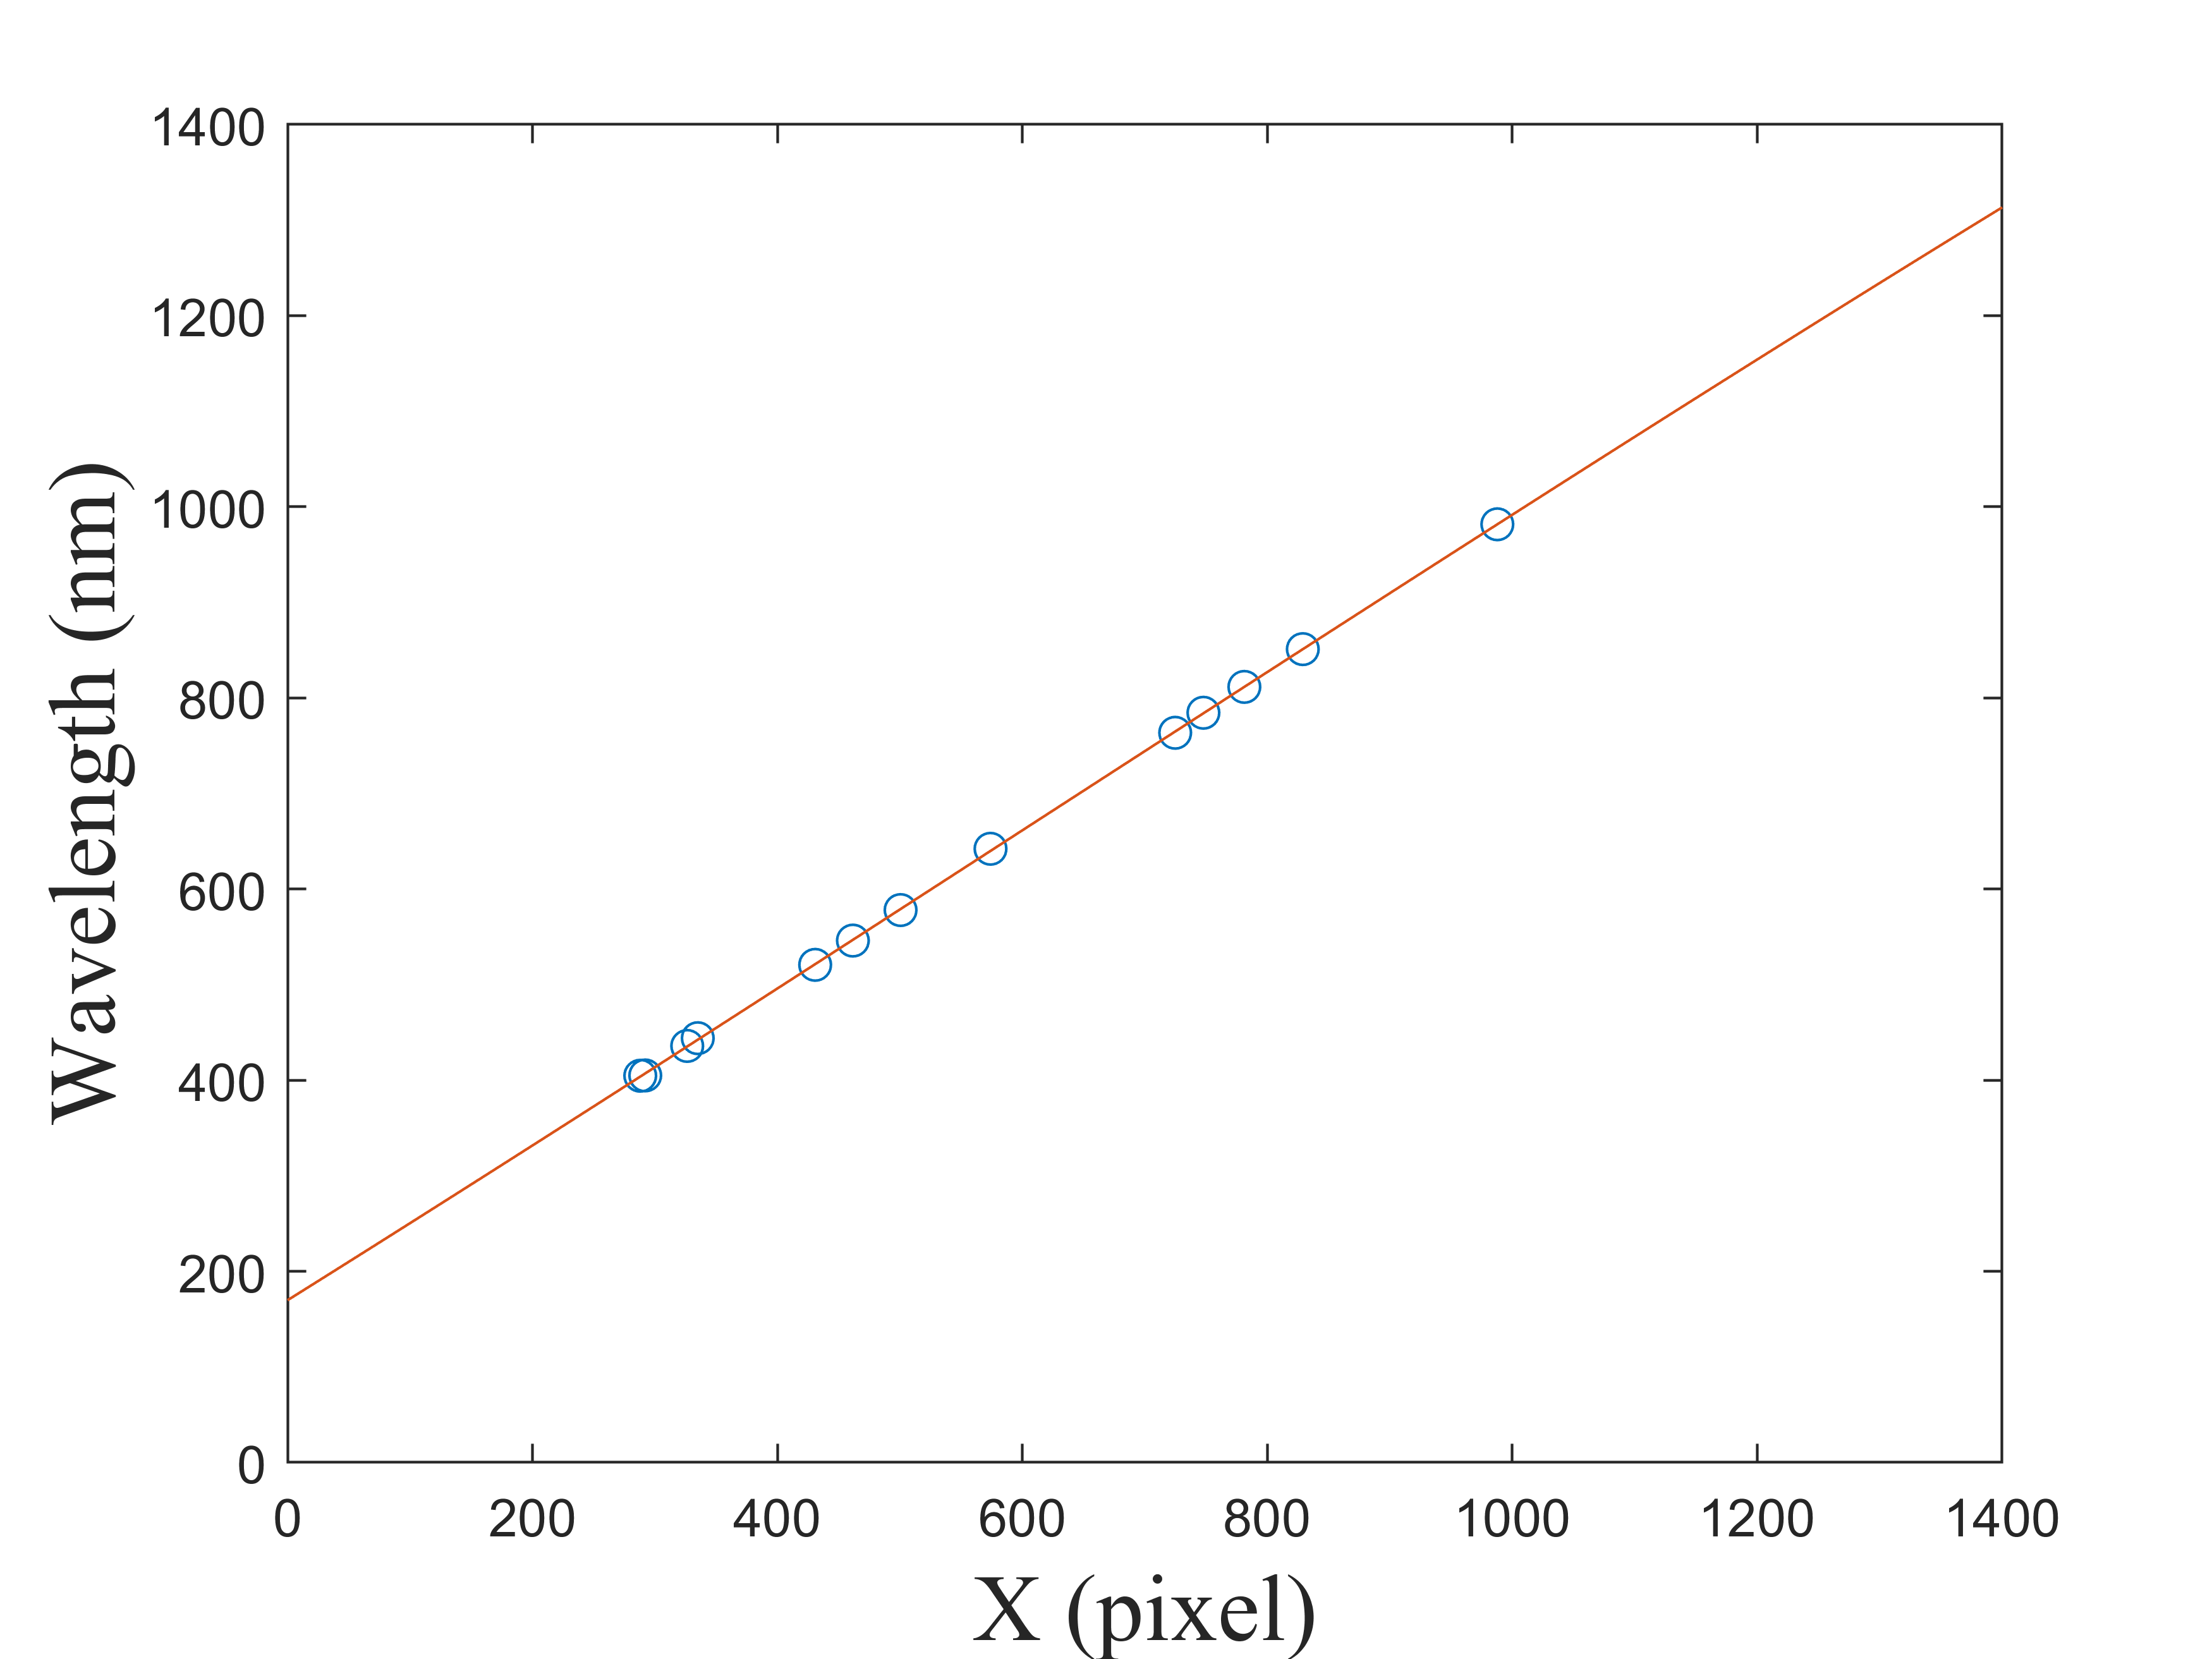
\includegraphics[width=16cm]{figures/COMBINE擬合結果.png} %插入图片,[]中设置图片大小,{}中是图片文件名
	\caption{空間轉換擬合曲線} %最终文档中希望显示的图片标题
	\label{空間轉換擬和曲線} %用于文内引用的标签
\end{figure}

\section{光譜晶片模組性能量化判定}
光譜晶片雖已經過波長校正,但並不能保證此光譜晶片品質優良,而光譜晶片的優劣將直接反映於光譜波形的表現上,汞氬燈這類原子光譜於理想的晶片下,半高全寬應趨近於零,而基線在不考慮電子雜訊干擾下,應平坦且趨近於零。\par
因晶片的性能優劣往往必須經由人工判定波形是否符合期待,但人工篩選常常參雜著主觀意見而標準不一,且耗時較長,因此為了使所有光譜晶片模組可以完全自動化校正並篩選,而在光源像素峰偵測流程時已計算出模型擬合與基線特徵點,因此本文提出將晶片性能以數值方式量化並提供篩選與判定。

\subsection{汞氬燈波形量化判定}
比較圖\ref{fig:all}. 中四張不同晶片之汞氬燈光譜,可以看出同樣於汞氬燈光源下,圖\ref{fig:a}. 晶片基線平整且半高全寬細,與其餘晶片的表現不同,顯然\ref{fig:d}. 晶片依然能以勞倫茲擬合後找出精準的波峰位置並波長校正,但圖\ref{fig:a}. 晶片波形表現明顯優於其餘晶片。

\begin{figure}[H]
	\vspace{0.8cm}
	\centering
	\begin{subfigure}[fig nice]{0.49\textwidth}
		\setlength{\abovecaptionskip}{0.cm}
		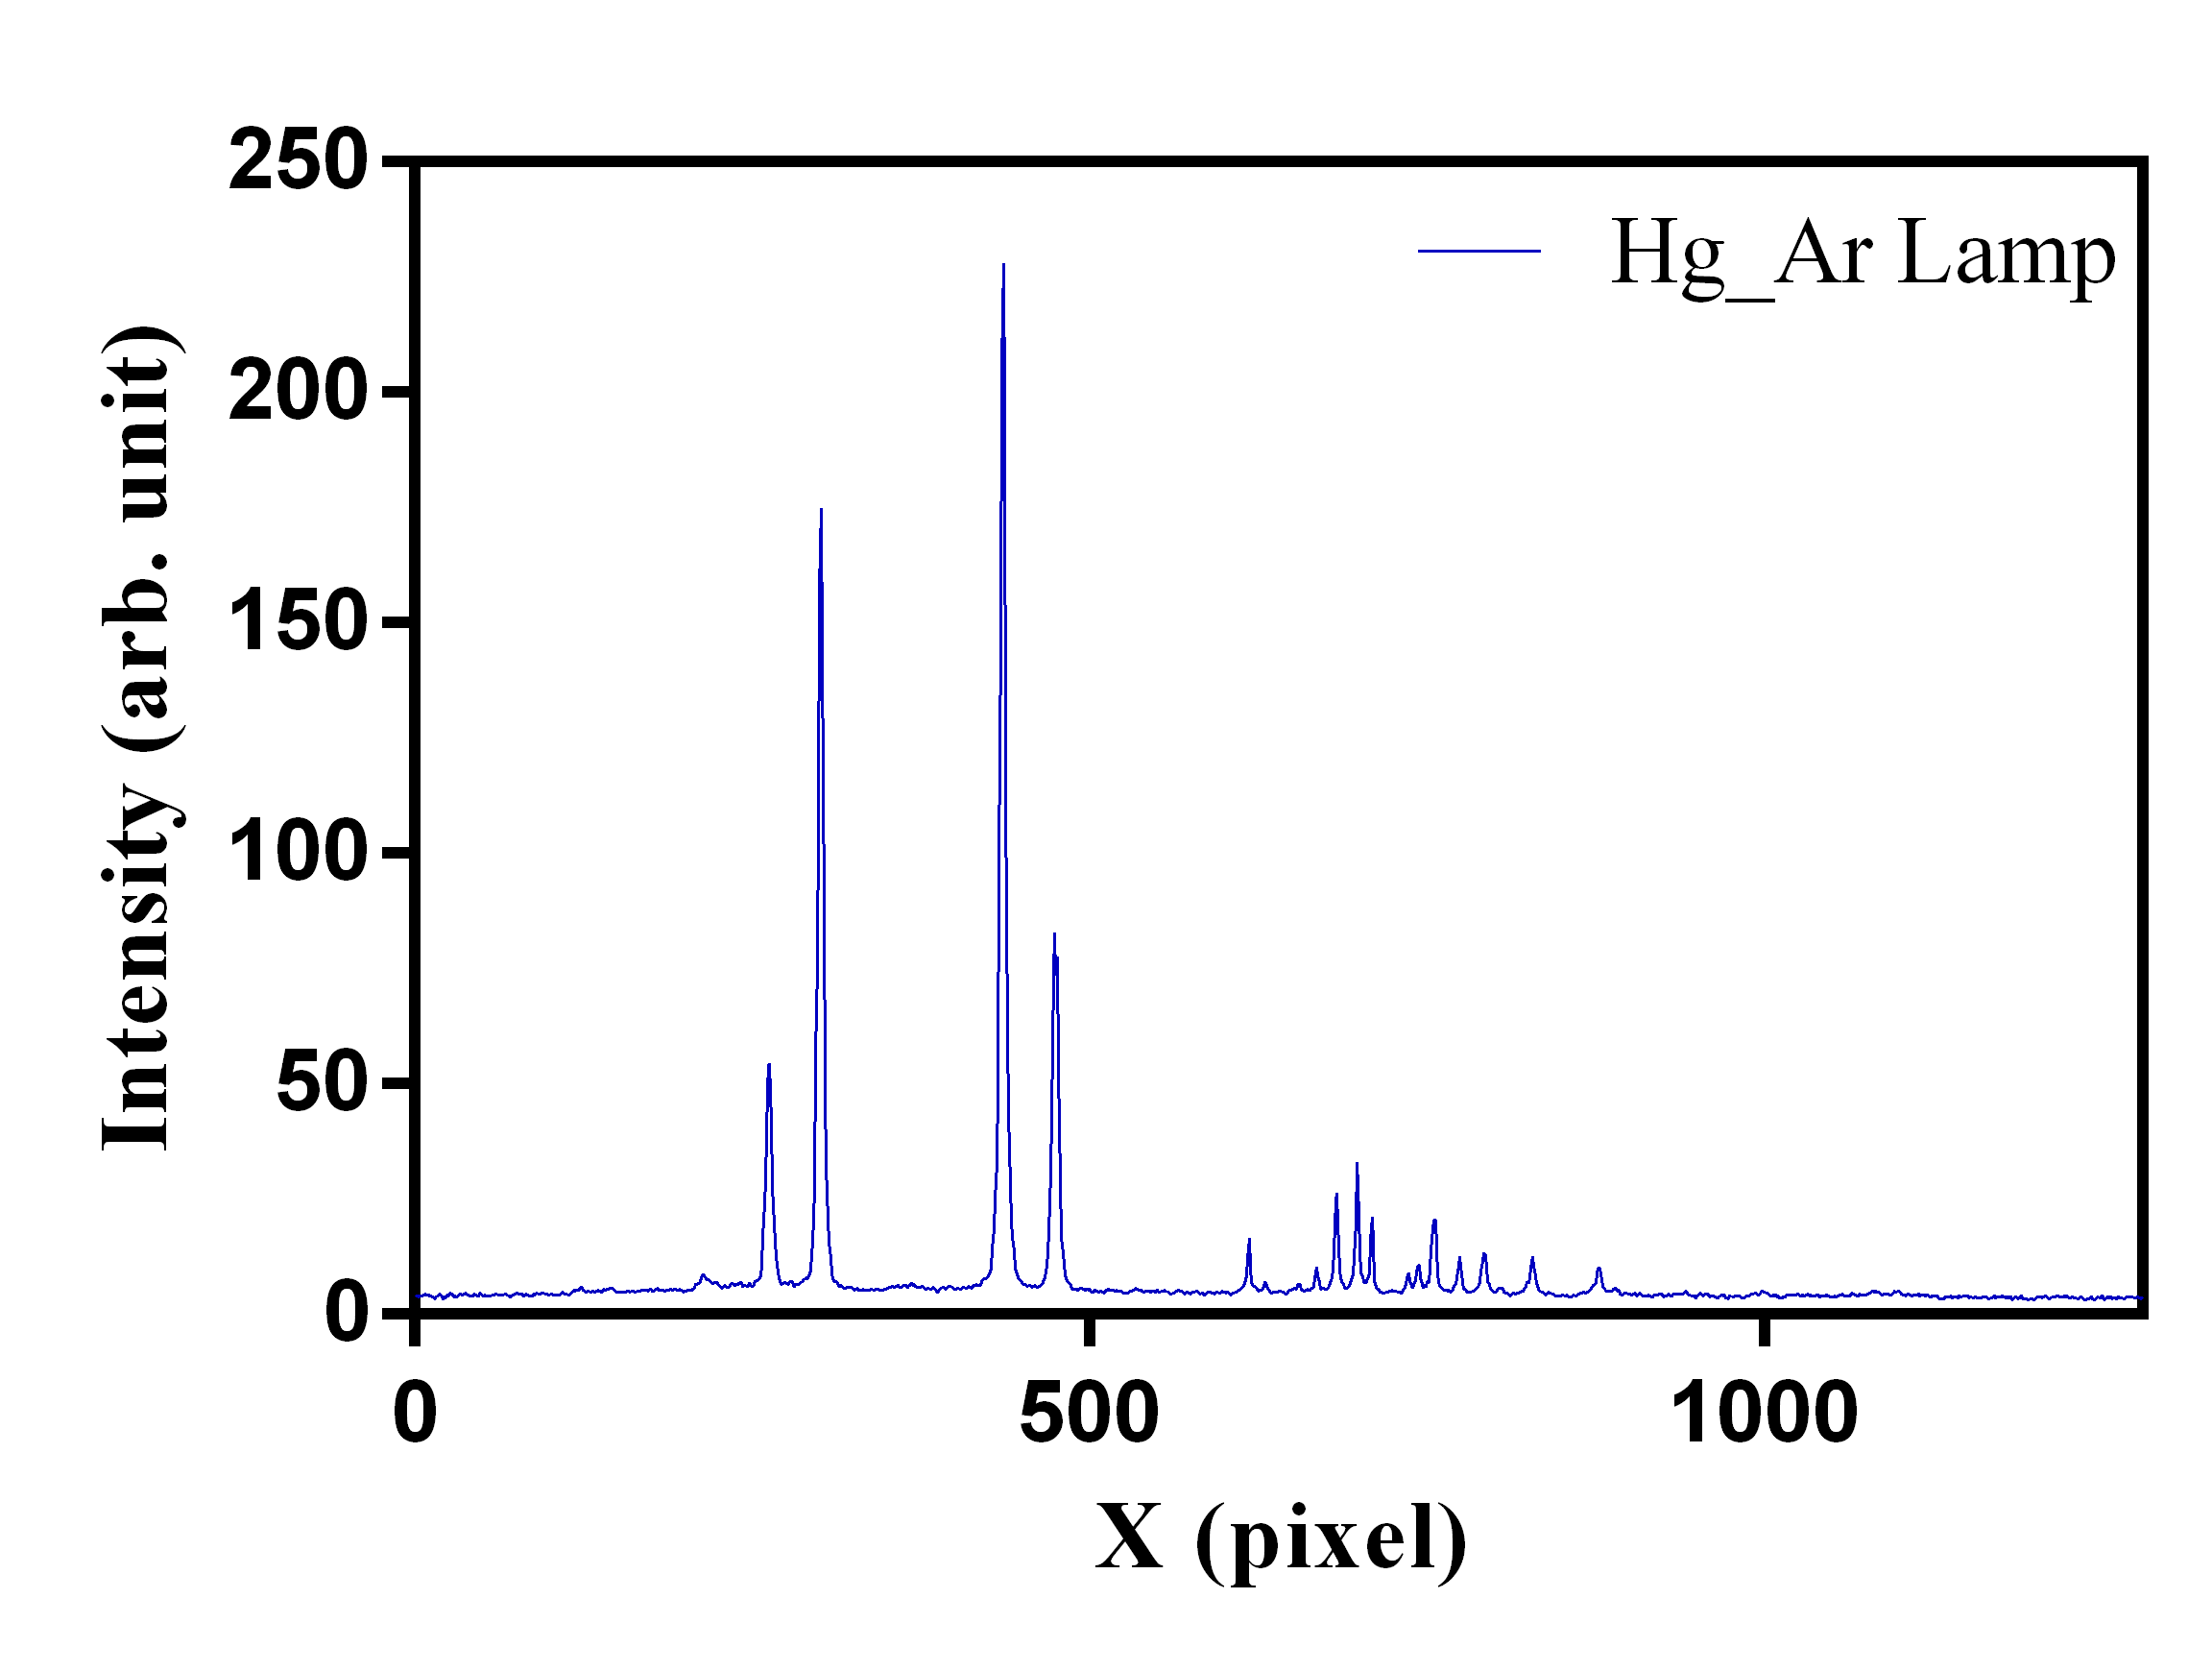
\includegraphics[width=7cm]{figures/hg_Nice.png}
		%\caption{優良晶片之汞氬燈光譜表現}
		\caption{}
		\label{fig:a}
	\end{subfigure}
\begin{subfigure}[fig nice]{0.49\textwidth}
	\setlength{\abovecaptionskip}{0.cm}
	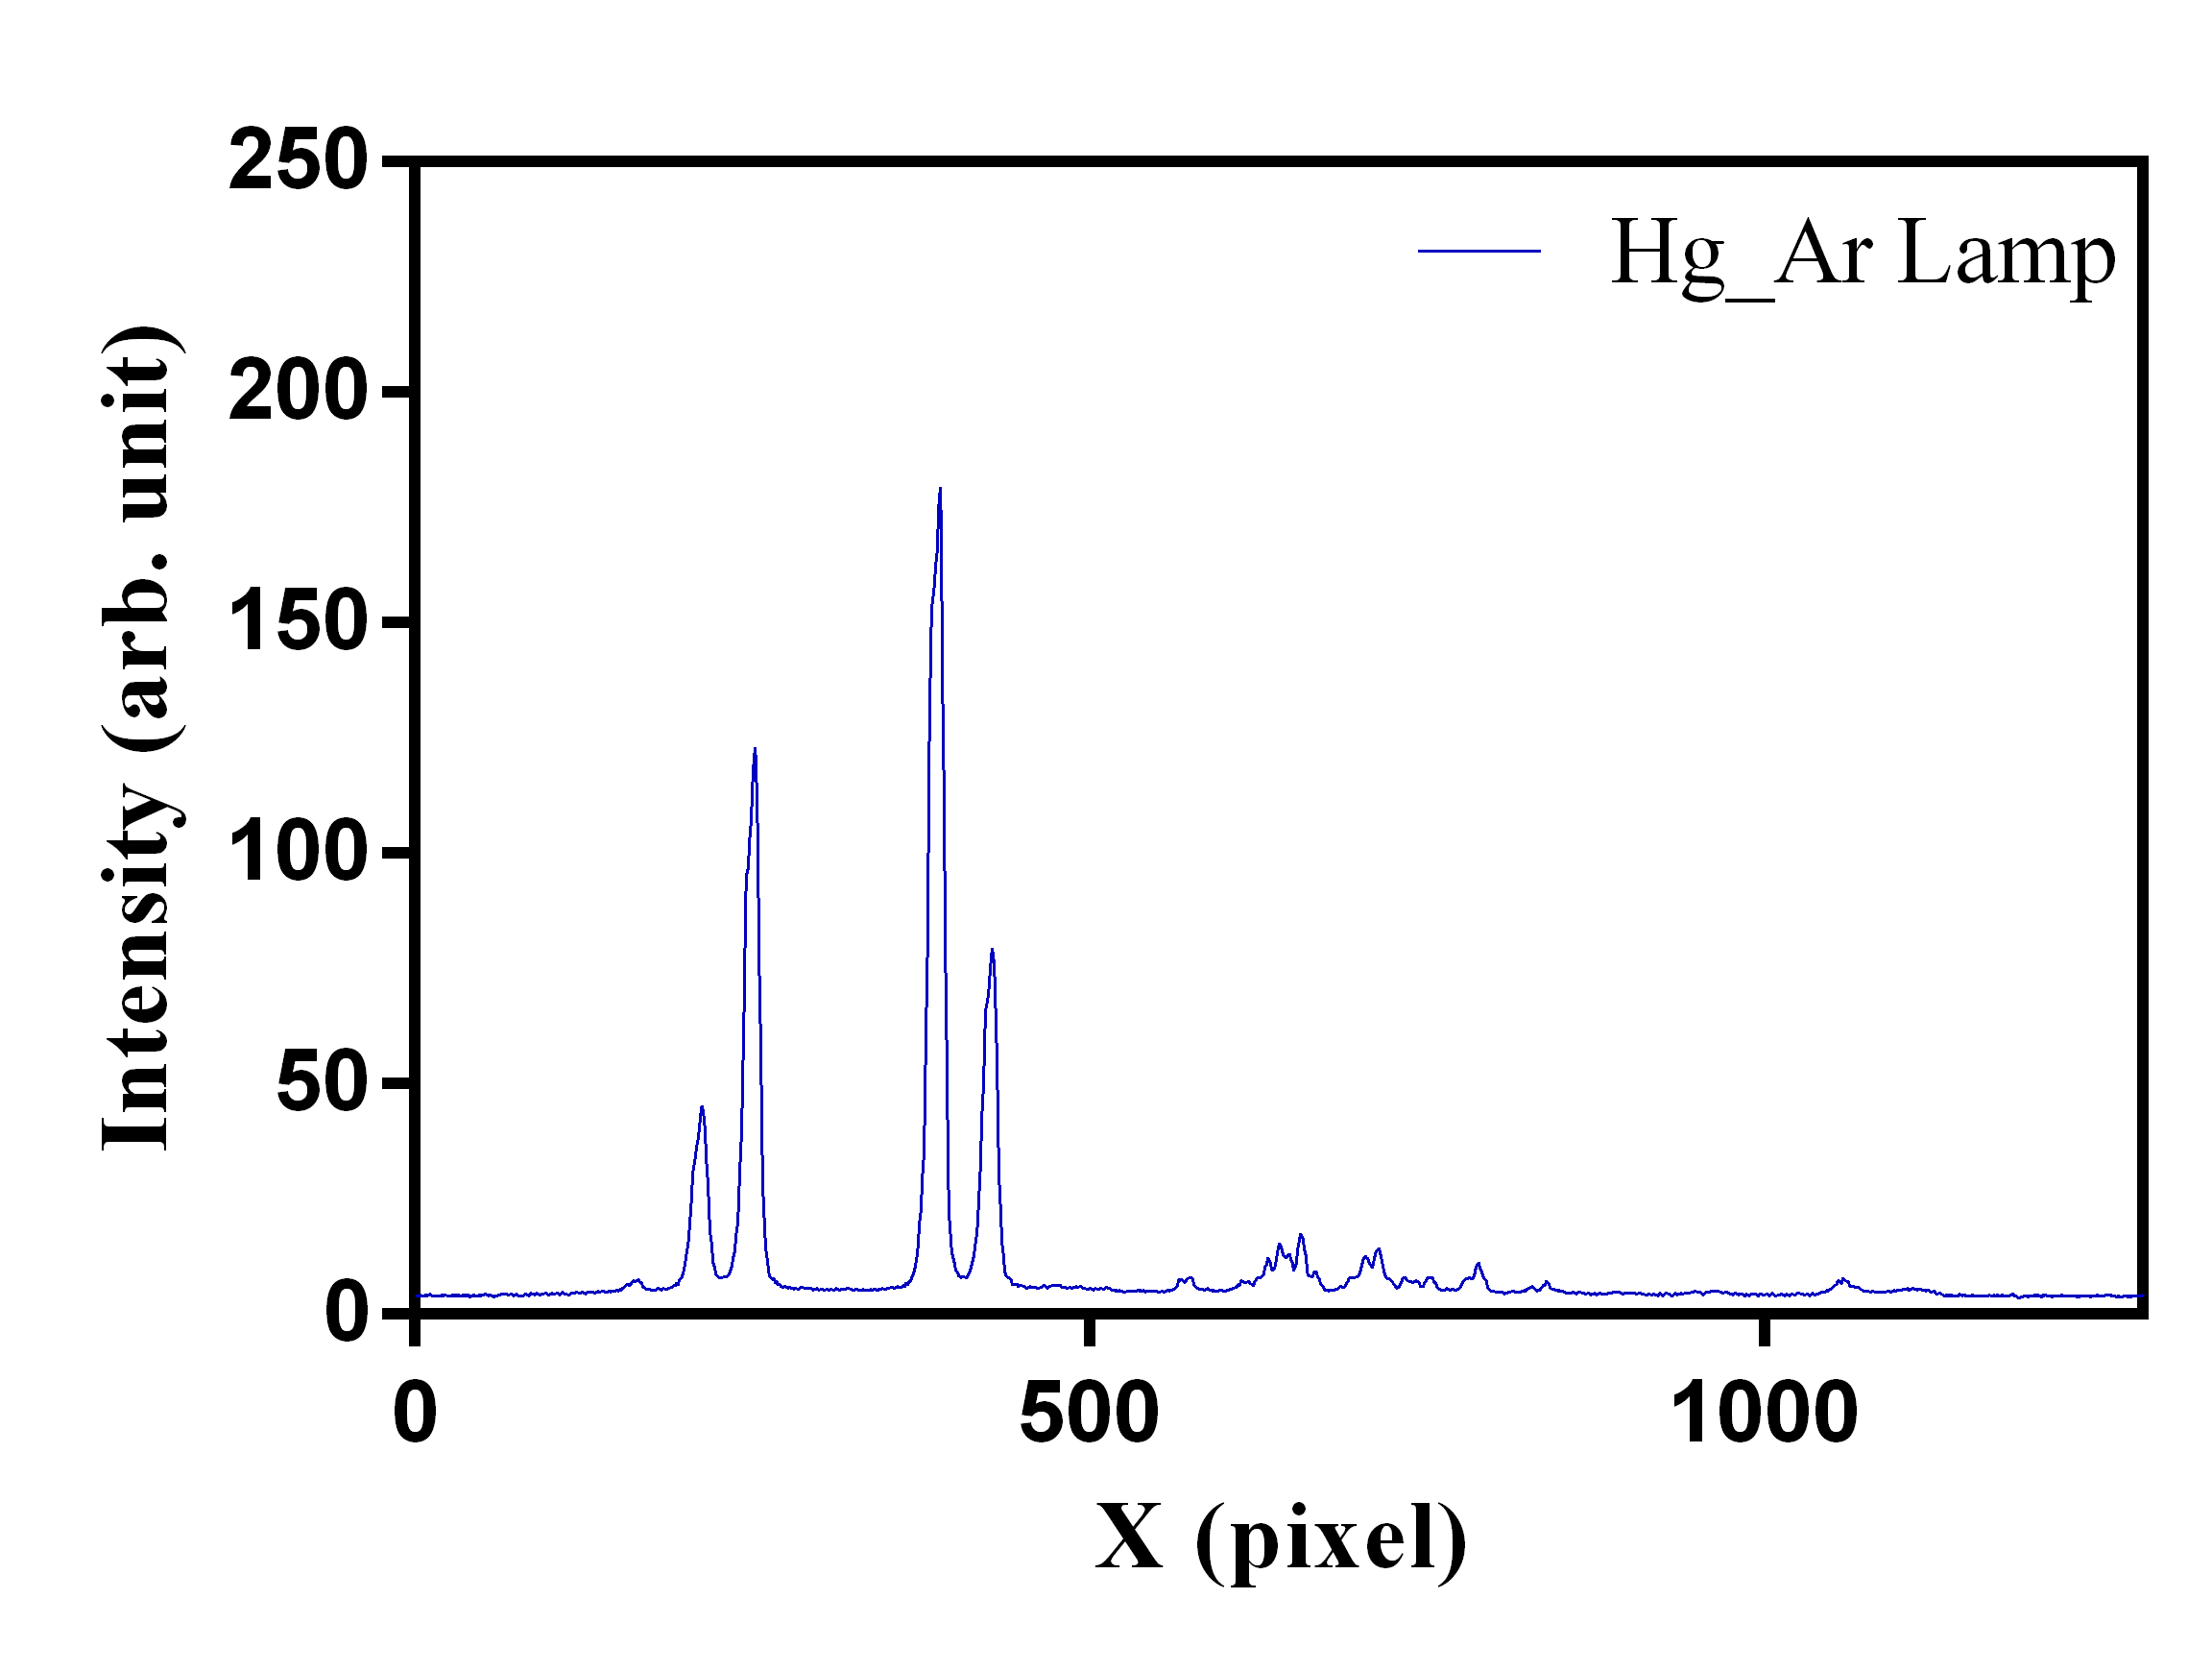
\includegraphics[width=7cm]{figures/hg_HWHM_BAD.png}
	%\caption{半高全寬較寬}
	\caption{}
	\label{fig:b}
\end{subfigure}
\begin{subfigure}[fig a]{0.49\textwidth}
	\setlength{\abovecaptionskip}{0.cm}
	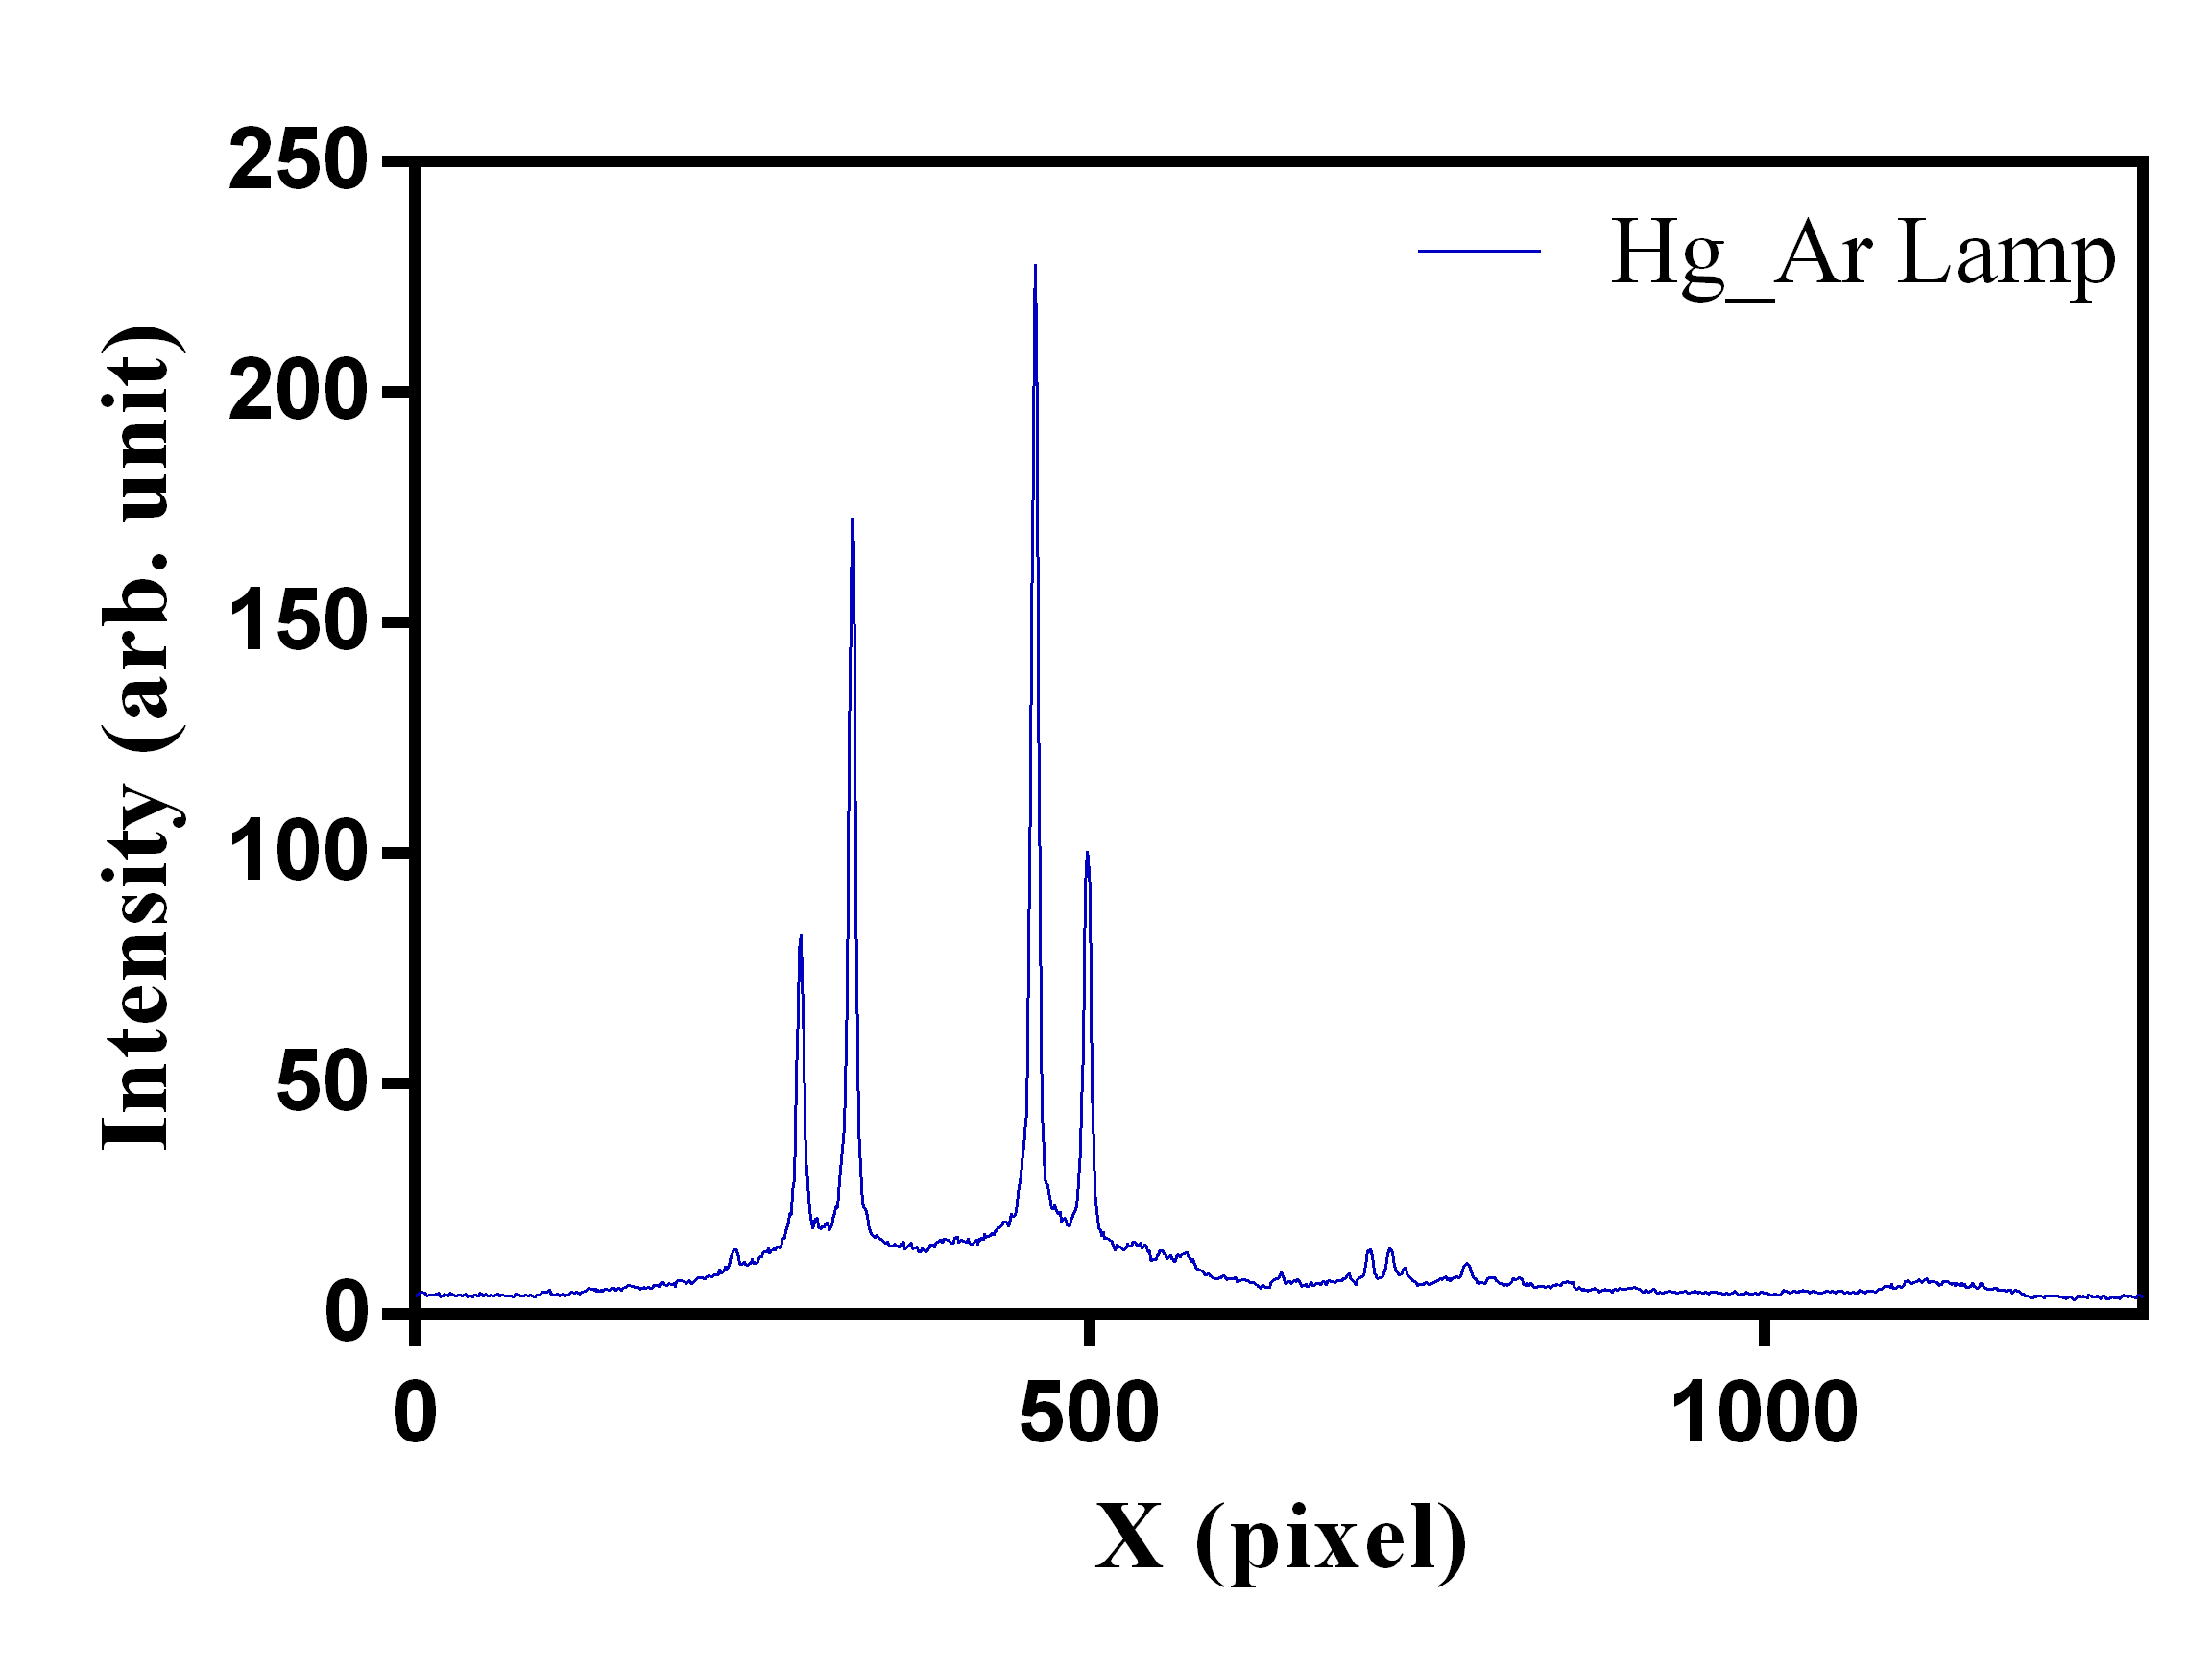
\includegraphics[width=7cm]{figures/hg_Baseline_bad.png}
	%\caption{基線較高}
	\caption{}
	\label{fig:c}
\end{subfigure}
\begin{subfigure}[fig b]{0.49\textwidth}
	\setlength{\abovecaptionskip}{0.cm}
	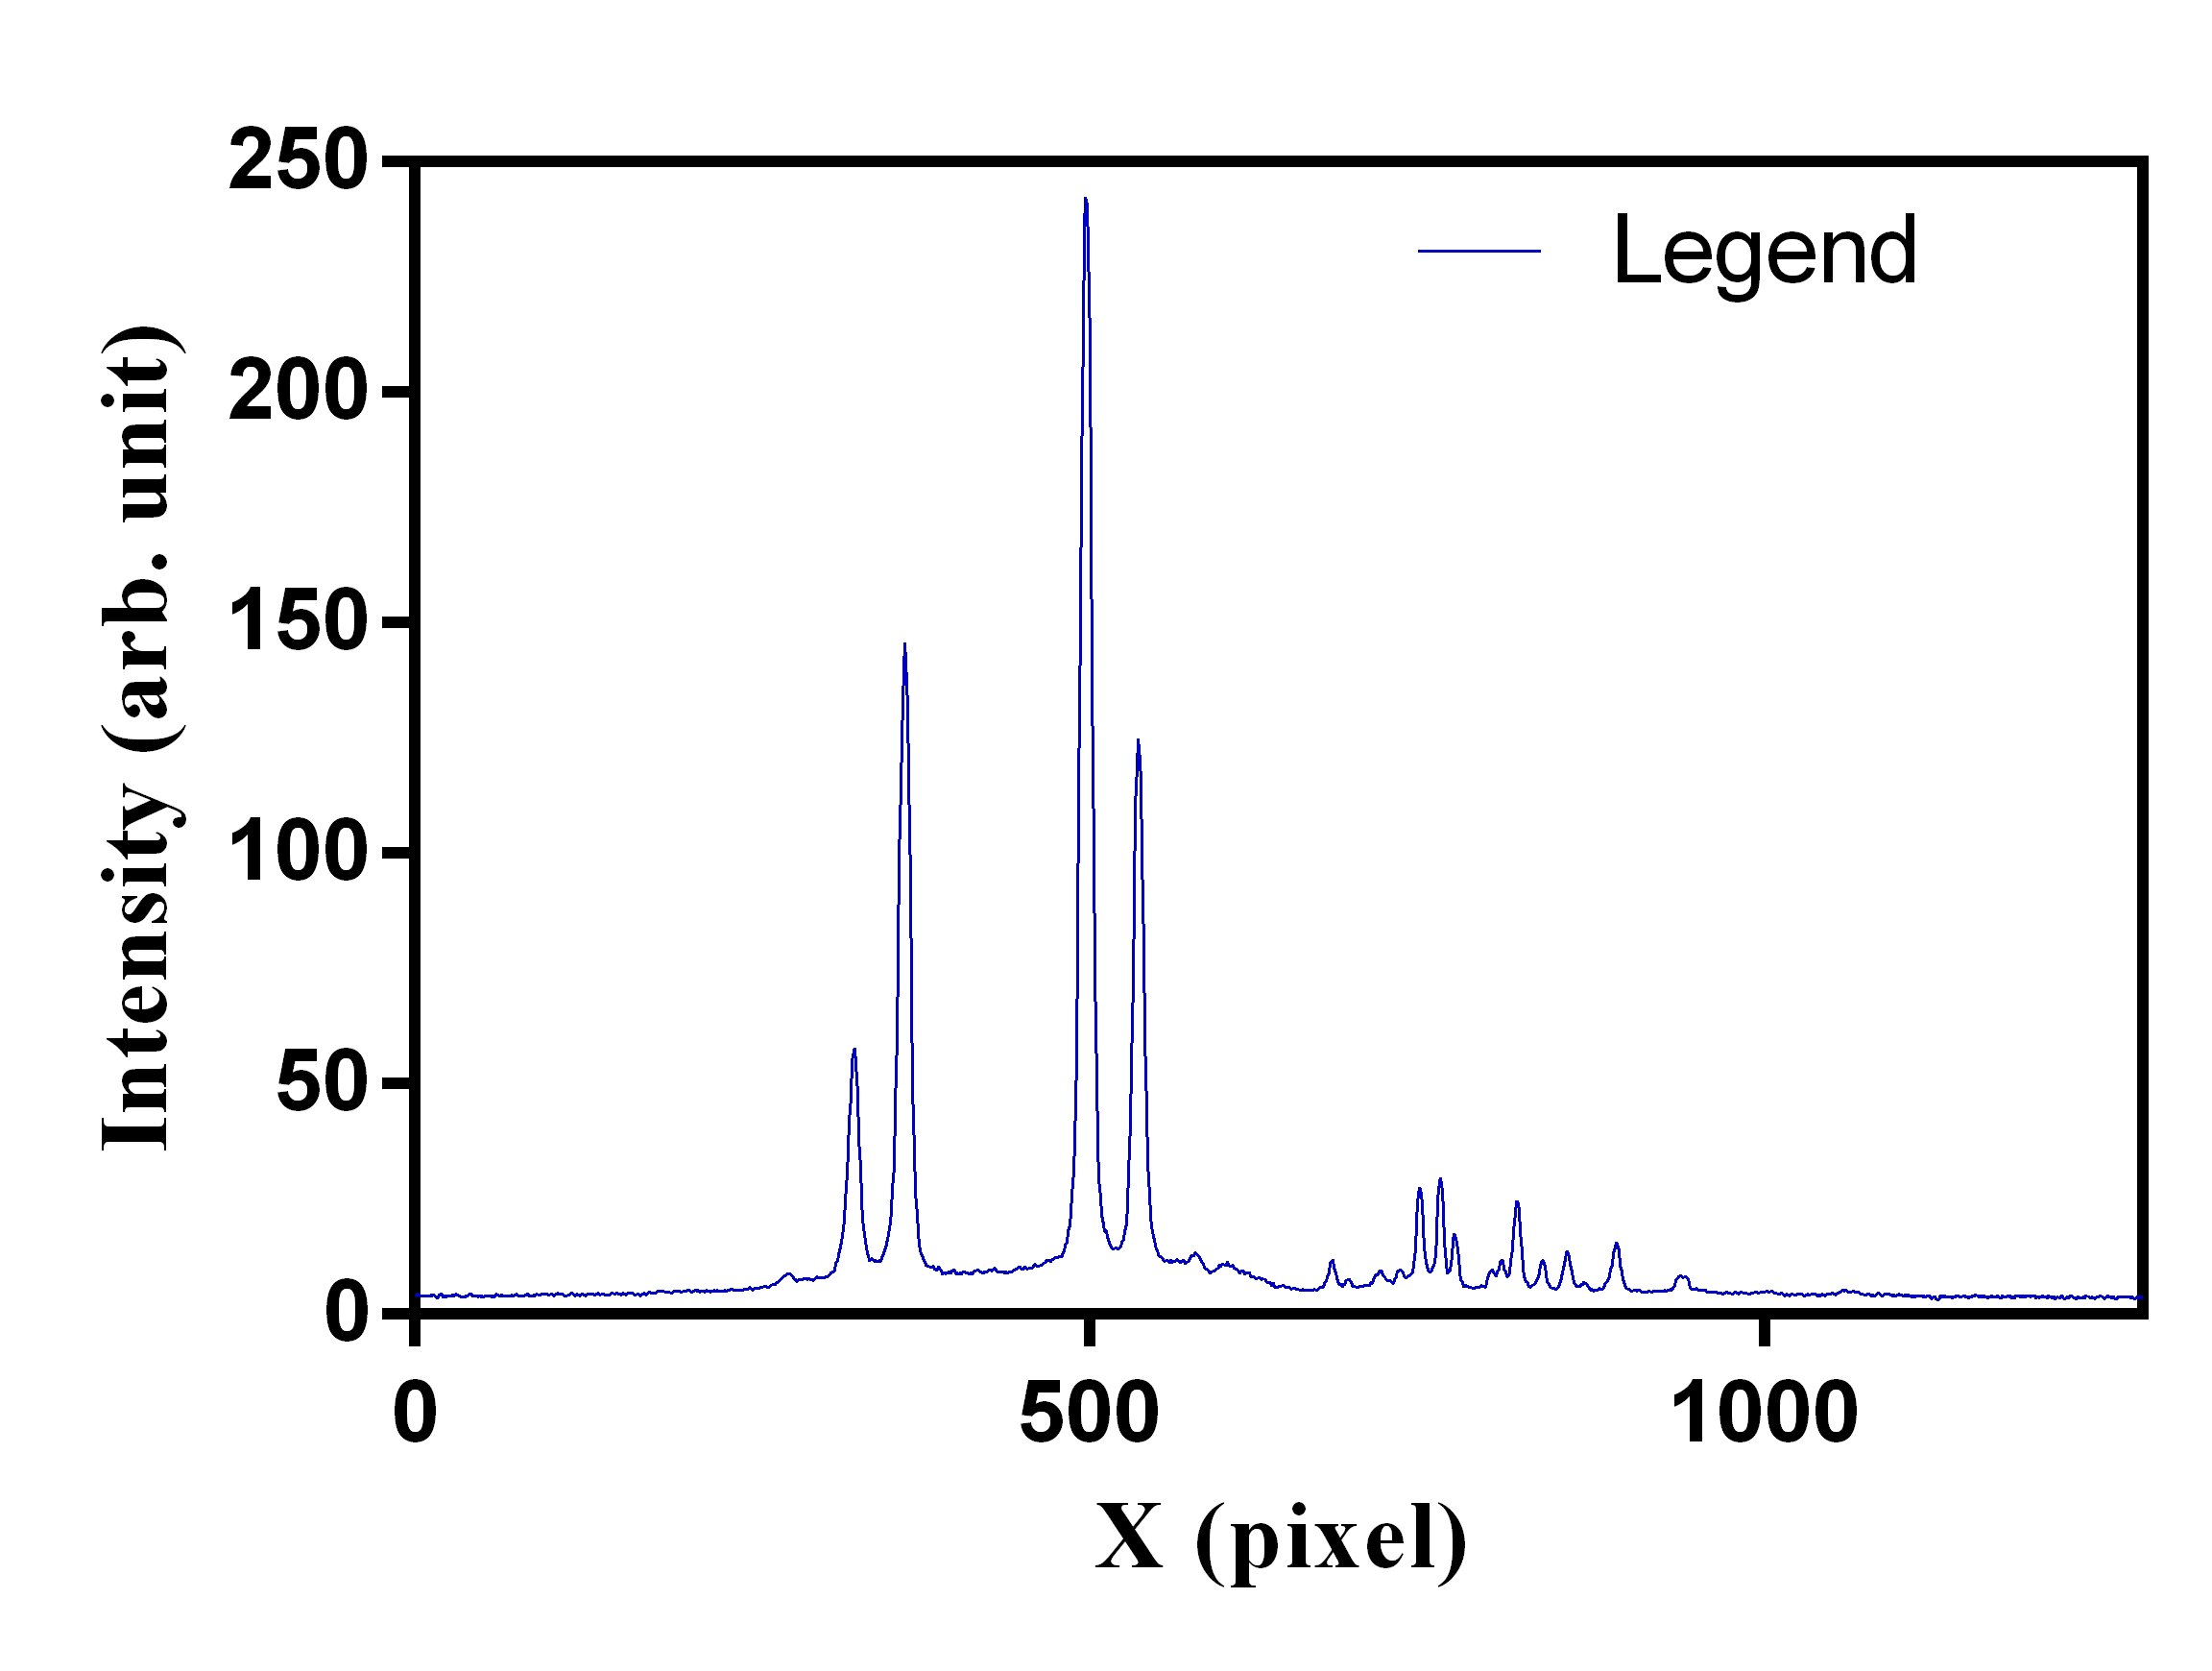
\includegraphics[width=7cm]{figures/hg_ar_4.png}
	%\caption{半高全寬與基線皆稍差}
	\caption{}
	\label{fig:d}
\end{subfigure}
\caption[汞氬燈於不同晶片的光譜表現]{汞氬燈於不同晶片下的光譜表現 (a)優良晶片光譜表現(b)半高全寬較寬(c)基線較高(d)半高全寬與基線皆稍差}
\label{fig:all}
\end{figure} 
由於汞氬燈之氬燈區光譜複雜且強度極低,對於量化判定相當困難,因此僅以汞燈區的波形表現判定,並將主要目標著重於判別基線是否升高,而晶片於較高波長時波形表現的優劣將以白光波形作為判定標準。\par
量化判定標準主要有汞氬燈之基線RMSE與半高全寬之RMSE,基線RMSE越大表示該晶片之基線升高程度越大,半高全寬之RMSE越大則代表該晶片解析度越差。量化判定需先將汞氬燈之汞燈區光譜數據透過3.5.1章所提到的分區方法分區並對各區域做勞倫茲擬合,並以小波轉換法求出基線,最後再將勞倫茲轉換後波形做基線補償得出結果,晶片間基線與波形優劣的差異如圖\ref{fig:all1}. 與圖\ref{fig:all2}. 所示。
\begin{figure}[H]
	\vspace{0.8cm}
	\centering
	\begin{subfigure}[fig nice]{0.49\textwidth}
		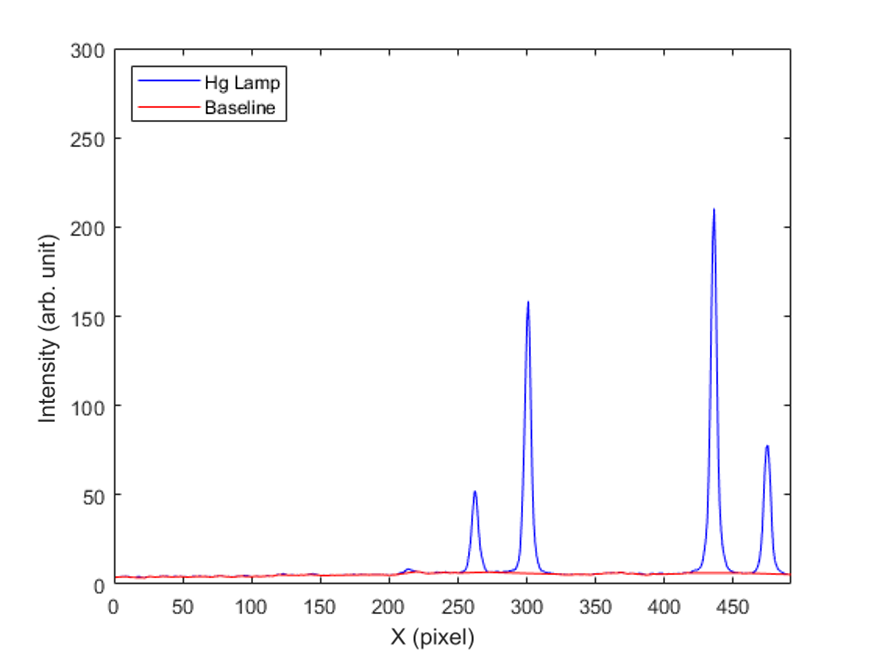
\includegraphics[width=7cm]{figures/nice_hg_base.png}
		\caption{}
		%\caption{基線表現優良晶片之汞燈光譜}
		\label{fig:a11}
	\end{subfigure}
	\begin{subfigure}[fig nice]{0.49\textwidth}
		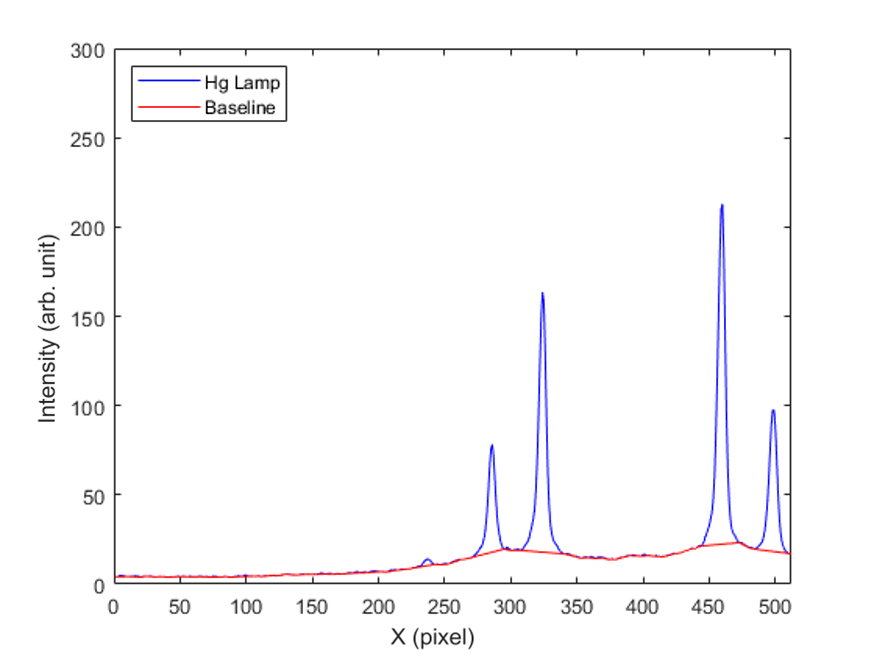
\includegraphics[width=7cm]{figures/badbase_hg_base.png}
		\caption{}
		%\caption{基線表現較差晶片之汞燈光譜}
		\label{fig:b12}
	\end{subfigure}
\begin{subfigure}[fig nice]{0.49\textwidth}
	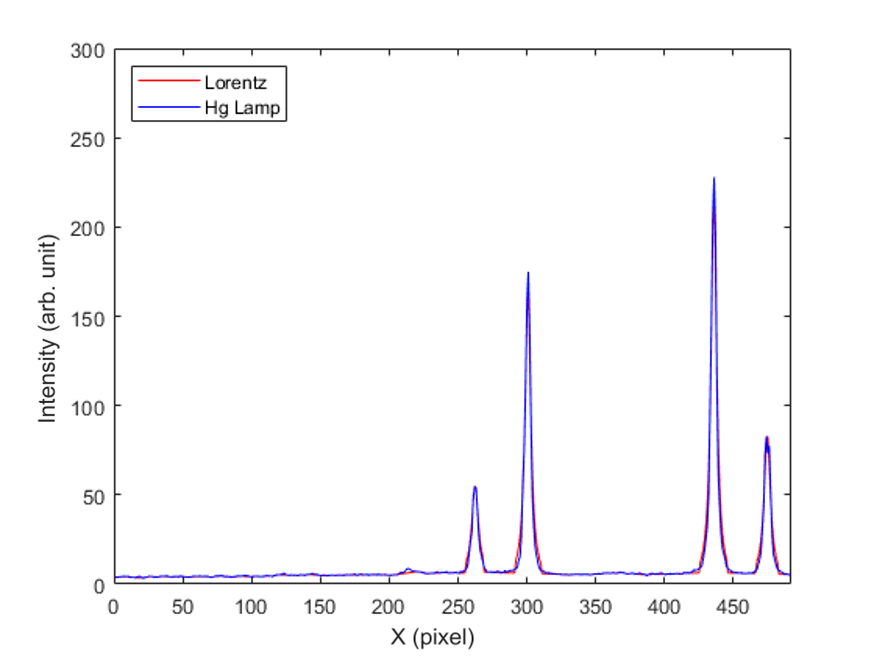
\includegraphics[width=7cm]{figures/nice_hg_lorentz.png}
	\caption{}
	%\caption{基線優良晶片勞倫茲擬合與基線補償結果}
	\label{fig:a13}
\end{subfigure}
\begin{subfigure}[fig nice]{0.49\textwidth}
	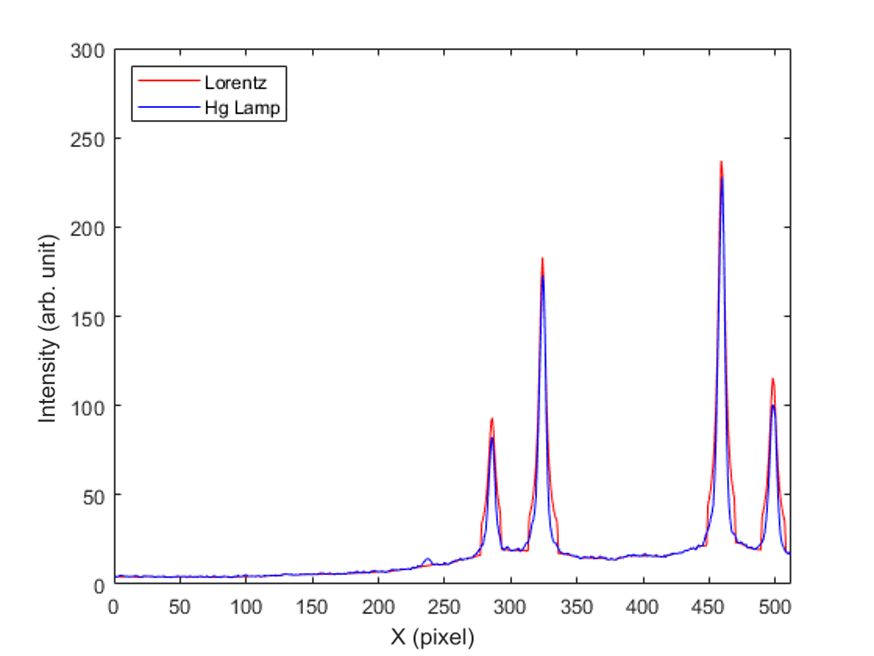
\includegraphics[width=7cm]{figures/badbase_hg_lorentz.png}
	\caption{}
	%\caption{基線較差晶片勞倫茲擬合與基線補償結果}
	\label{fig:b14}
\end{subfigure}
	\caption[波形優良但基線不佳之晶片比較]{波形優良但基線不佳之晶片比較 (a)基線表現優良晶片之汞燈光譜(b)基線表現較差晶片之汞燈光譜(c)基線優良晶片勞倫茲擬合與基線補償結果(d)基線較差晶片勞倫茲擬合與基線補償結果}
	\label{fig:all1}
\end{figure} 
如圖\ref{fig:all1}. 所示,比較圖\ref{fig:a11}. 與圖\ref{fig:b12}. 可看出圖\ref{fig:b12}. 晶片的基線升高現象相當嚴重,因此基線判定對於一個晶片的性能良好與否至關重要,而由圖\ref{fig:a13}. 與圖\ref{fig:b14}. 中可以看出性能優良的晶片,不僅基線穩定且逼近於零,在勞倫茲擬合並且基線補償後的半高全寬與波形表現皆非常優良。
\begin{figure}[H]
	\centering
	\begin{subfigure}[fig nice]{0.49\textwidth}
		\includegraphics[width=7cm]{figures/nice_hg_base.png}
		\caption{}
		%\caption{波形優良之晶片基線表現}
		\label{fig:a21}
	\end{subfigure}
	\begin{subfigure}[fig nice]{0.49\textwidth}
		\includegraphics[width=7cm]{figures/bad_hg_base.png}
		\caption{}
		%\caption{波形較差之晶片基線表現}
		\label{fig:b22}
	\end{subfigure}
\begin{subfigure}[fig nice]{0.49\textwidth}
	\includegraphics[width=7cm]{figures/nice_hg_lorentz.png}
	\caption{}
	%\caption{波形優良晶片勞倫茲擬合與基線補償結果}
	\label{fig:a23}
\end{subfigure}
\begin{subfigure}[fig nice]{0.49\textwidth}
	\includegraphics[width=7cm]{figures/bad_hg_lorentz.png}
	\caption{}
	%\caption{波形較差晶片勞倫茲擬合與基線補償結果}
	\label{fig:b24}
\end{subfigure}
	\caption[基線優良但波形不佳之晶片比較]{基線優良但波形不佳之晶片比較 (a)波形優良之晶片基線表現(b)波形較差之晶片基線表現(c)波形優良晶片勞倫茲擬合與基線補償結果(d)波形較差晶片勞倫茲擬合與基線補償結果}
	\label{fig:all2}
\end{figure}  
如圖\ref{fig:all2}. 所示,由圖\ref{fig:a21}. 與圖\ref{fig:b22}. 比較可看出雖然兩個晶片的基線升高現象都非常輕微,但由圖\ref{fig:a23}. 與圖\ref{fig:b24}. 中可以看出勞倫茲擬合後圖\ref{fig:b24}. 之半高全寬相當大,因此不僅需將基線升高現象做為晶片效能優良與否判斷,勞倫茲擬合後的半高全寬也是晶片效能的重要參考點。

\subsection{白光LED波形量化判定}
不同於汞氬燈光譜波形的多個獨立錐狀,且峰與峰間有無信號區,白光光譜如圖\ref{白光LED光譜}. 所示,橫跨幾乎所有可見光波段,又因其光譜波形連續不中斷,因此比起汞氬燈更能體現出晶片的光譜表現。\par
白光LED為藍光晶粒激發黃色螢光而產生白光,因此藍光與黃光相互影響作用,且因白光連續不中斷,造成難以判定是否有基線升高現象,而基線已於汞氬燈時判定,因此白光LED量化判定著重於判定整個可見光波段中光譜波形表現。\par
\begin{figure}[H] %H为当前位置,!htb为忽略美学标准,htbp为浮动图形
	\centering %图片居中
	\vspace{0.8cm}
	\setlength{\abovecaptionskip}{0.cm}
	\includegraphics[width=\textwidth]{figures/White_wavelenght.png} %插入图片,[]中设置图片大小,{}中是图片文件名
	\caption{白光LED光譜} %最终文档中希望显示的图片标题
	\label{白光LED光譜} %用于文内引用的标签
\end{figure}
白光LED模型擬合如表\ref{光源介紹表}. 所示,需同時以兩種不同模型表示。本文先將光譜拆為兩段分析,藍光LED晶粒產生的光譜為躍遷光譜,躍遷光譜極逼近於勞倫茲函數模型,而受激發而發亮的黃色螢光粉則逼近於高斯函數模型,首先將白光LED以3.5.1章所提的分區方法將白光數據切割,並將第一區間的藍光光譜以勞倫茲模型擬合,如圖\ref{藍光區域以勞倫茲模型擬合結果}. 所示。
\begin{figure}[H] %H为当前位置,!htb为忽略美学标准,htbp为浮动图形
	\centering %图片居中
	%\setlength{\abovecaptionskip}{1cm}
	\includegraphics[width=16cm]{figures/white_lorentz.png} %插入图片,[]中设置图片大小,{}中是图片文件名
	\caption{藍光區域以勞倫茲模型擬合結果} %最终文档中希望显示的图片标题
	\label{藍光區域以勞倫茲模型擬合結果} %用于文内引用的标签
\end{figure}
由於藍光波形與黃色螢光波形相互影響作用,而藍光因強度較螢光強上許多,因此受黃色螢光影響較小,可以直接以勞倫茲模型擬合逼近,而因黃色螢光較弱,所以受到藍光的影響,造成黃色螢光前端的強度攀升區域的波形與藍光耦合,若直接以高斯模型擬合將會產生較大誤差。\par
圖\ref{藍光區域以勞倫茲模型擬合結果}. 為透過擬合得出勞倫茲方程式後,將像素帶入方程式估算出藍光光譜的延伸波形。將白光光譜扣除藍光對於後方螢光區域的影響後,螢光區的光譜就可以使用高斯函數逼近,逼近後結果如圖\ref{螢光區域以高斯模型擬合結果}. 所示。
\begin{figure}[H] %H为当前位置,!htb为忽略美学标准,htbp为浮动图形
	\centering %图片居中
	%\setlength{\abovecaptionskip}{1cm}
	\includegraphics[width=16cm]{figures/white_gaussian.png} %插入图片,[]中设置图片大小,{}中是图片文件名
	\caption{螢光區域以高斯模型擬合結果} %最终文档中希望显示的图片标题
	\label{螢光區域以高斯模型擬合結果} %用于文内引用的标签
\end{figure}
兩區域數據處理並擬合後,將圖\ref{螢光區域以高斯模型擬合結果}. 中的高斯模型函數往前延伸並求出與勞倫茲函數模型的交點,並以此點做為結合點將兩模型組合為白光LED光譜的理想參考波形。\par
圖\ref{雙模型擬合結果}. 為實際對晶片以白光LED做量化判定的結果,並標示透過兩模型擬合後所得出的半高全寬與原始數據對參考波形的總體RMSE,此兩項數據可提供使用者做為晶片優劣的量化判定值。
\begin{figure}[H] %H为当前位置,!htb为忽略美学标准,htbp为浮动图形
	\centering %图片居中
	%\setlength{\abovecaptionskip}{1cm}
	\includegraphics[width=\textwidth]{figures/20C4-203-D1.png} %插入图片,[]中设置图片大小,{}中是图片文件名
	\caption{雙模型擬合結果} %最终文档中希望显示的图片标题
	\label{雙模型擬合結果} %用于文内引用的标签
\end{figure}
% !TeX root = ../main.tex
\titlespacing{\chapter}{0cm}{-2cm}{0cm}
\chapter{實驗結果}


\section{實際晶片量測}
演算法於電腦上通過RS-232\cite{RS232}控制光源,對光譜晶片模組進行波長校正,ROI Scan後結果如圖\ref{fig:ROI SCAN 1}. 所示,精準的找到光源的ROI區域。

\begin{figure}[H]
	\vspace{0.8cm}
	\centering
	\begin{subfigure}[fig nice]{0.328\textwidth}
		\includegraphics[width=4.9cm]{figures/Result/20C4-205-C4_full_Image__Hg_Ar_2021-05-10-16-25.jpg}
		\caption{}
		%\caption{汞氬燈}
		\label{fig:image_HG1}
	\end{subfigure}
	\begin{subfigure}[fig nice]{0.328\textwidth}
		\includegraphics[width=4.9cm]{figures/Result/20C4-205-C4_full_Image__Laser8_2021-05-10-16-28.jpg}
		\caption{}
		%\caption{雷射}
		\label{fig:image_LASER1}
	\end{subfigure}
	\begin{subfigure}[fig nice]{0.328\textwidth}
		\includegraphics[width=4.9cm]{figures/Result/20C4-205-C4_full_Image__White_2021-05-10-16-30.jpg}
		\caption{}
		%\caption{白光LED}
		\label{fig:image_White1}
	\end{subfigure}
	\caption[同一晶片下不同光源的ROI SCAN結果圖]{同晶片不同光源ROI SCAN結果 (a)汞氬燈(b)雷射(c)白光LED}
	\label{fig:ROI SCAN 1}
\end{figure} 
在同一晶片下,通過將ROI區域影像中所有像素點帶入式(\ref{eq:2.4})計算得出如式(\ref{RGB:3.9})之光譜數據矩陣後,繪出光譜圖。汞氬燈、雷射與白光各自的光譜波形圖如圖\ref{fig:Spectrum 1}. 所示。
\begin{figure}[H]
	\vspace{0.8cm}
	\centering
	\begin{subfigure}[fig nice]{0.328\textwidth}
		\includegraphics[width=4.9cm]{figures/Result/20C4-205-C4_HgAr.PNG}
		\caption{}
		%\caption{汞氬燈}
		\label{fig:Spectrum_HG1}
	\end{subfigure}
	\begin{subfigure}[fig nice]{0.328\textwidth}
		\includegraphics[width=4.9cm]{figures/Result/20C4-205-C4_Laser.PNG}
		\caption{}
		%\caption{七根單雷射疊圖}
		\label{fig:Spectrum_LASER1}
	\end{subfigure}
	\begin{subfigure}[fig nice]{0.328\textwidth}
		\includegraphics[width=4.9cm]{figures/Result/20C4-205-C4_White.PNG}
		\caption{}
		%\caption{白光LED}
		\label{fig:Spectrum_White1}
	\end{subfigure}
	\caption[同一晶片下不同光源的光譜圖形]{同晶片不同光源的光譜圖形 (a)汞氬燈(b)七根單雷射疊圖(c)白光LED}
	\label{fig:Spectrum 1}
\end{figure} 
\newpage
經演算法計算後汞氬燈與雷射峰值偵測與波長校正三次多項式擬合的結果如圖\ref{峰值偵測與三次多項式擬合結果}. 所示。汞氬燈光譜波形量化結果,如圖\ref{汞燈光譜量化}. 所示。白光光譜波形量化結果,如圖\ref{白光光譜量化}. 所示。晶片參數如表\ref{不同晶片汞氬燈校正結果參數}. 所示。
\begin{figure}[H] %H为当前位置,!htb为忽略美学标准,htbp为浮动图形
	\centering %图片居中
	\vspace{0.8cm}
	%\setlength{\abovecaptionskip}{1cm}
	\includegraphics[width=0.74\textwidth]{figures/Result/Result_2021-05-10-16-29-08.jpg} %插入图片,[]中设置图片大小,{}中是图片文件名
	\caption{峰值偵測與三次多項式擬合結果} %最终文档中希望显示的图片标题
	\label{峰值偵測與三次多項式擬合結果} %用于文内引用的标签
\end{figure}
\begin{figure}[H] %H为当前位置,!htb为忽略美学标准,htbp为浮动图形
	\centering %图片居中
	\vspace{0.8cm}
	%\setlength{\abovecaptionskip}{1cm}
	\includegraphics[width=0.74\textwidth]{figures/Result/Result_2021-05-10-16-24-49.jpg} %插入图片,[]中设置图片大小,{}中是图片文件名
	\caption{汞燈光譜量化} %最终文档中希望显示的图片标题
	\label{汞燈光譜量化} %用于文内引用的标签
\end{figure}
\begin{figure}[H] %H为当前位置,!htb为忽略美学标准,htbp为浮动图形
	\centering %图片居中
	\vspace{0.8cm}
	%\setlength{\abovecaptionskip}{1cm}
	\includegraphics[width=0.74\textwidth]{figures/Result/Result_2021-05-10-16-30-57.jpg} %插入图片,[]中设置图片大小,{}中是图片文件名
	\caption{白光光譜量化} %最终文档中希望显示的图片标题
	\label{白光光譜量化} %用于文内引用的标签
\end{figure}
\begin{center}
	\vspace{0.8cm}
	\captionof{table}{晶片20C4-205-C4校正結果參數表}\label{不同晶片汞氬燈校正結果參數}
\begin{tabularx}{\textwidth}{cccccccc}
	\hline\hline
	\multicolumn{8}{c}{空間轉換方程式}\\
	\hline
	\multicolumn{8}{c}{$\lambda_i = 161.702366565752 + 0.76016P_i + 12.26498\times 10^{-5}P_i^2 -6.16582\times 10^{-8}P_i^3$}\\
	\hline
	\multirow{2}{*}{光源}
	&峰值位置&標準波長&轉換波長&誤差&半高全寬&半高全寬&解析度\\
	&(pixel)&(nm)&(nm)&(nm)&(pixel)&(nm)&(nm)\\
	\hline
	\multirow{4}{*}{汞燈 }
	&304.42&404.65&404.59&-0.06&5.81&4.76&5.18\\
	&342.70&435.83&435.91&0.08&6.32&5.17&5.18\\
	&477.45&546.07&546.10&0.03&6.49&5.32&5.18\\
	&516.24&578.01&577.93&-0.08&6.61&5.43&5.18\\
	\hline
	\multirow{2}{*}{氬燈 }
	&738.97&763.51&763.57&0.06&6.49&5.51&5.18\\
	&795.04&811.53&811.49&0.04&7.30&6.28&5.18\\  
	\hline	
	雷射1&311.41&404.97&406.21&1.24&5.09&4.26&4.18\\
	雷射2&353.37&443.93&441.41&-2.52&5.13&4.31&4.18\\
	雷射3&449.50&520.69&522.45&1.76&5.49&4.64&4.18\\
	雷射5&591.20&642.13&642.35&0.22&5.45&4.61&4.18\\
	雷射6&756.55&784.46&781.74&-2.72&6.39&5.35&4.18\\
	雷射7&842.54&851.04&853.50&2.46&5.43&4.51&4.18\\
	雷射8&998.17&981.67&981.25&-0.42&6.44&5.21&4.18\\
	\hline\hline
\end{tabularx}
\end{center}
\newpage
\section{不同方法之波長校正比較}
將多個不同晶片的量測進行進一步比較,波長校正參數由汞氬燈與雷射此兩光源所提供的波峰進行擬合,比較單純以汞氬燈或雷射波峰進行波長校正的準確度,與使用雙光源所提供的波峰進行的波長校正的準確度的差異。\par
汞氬燈波峰偵測與三次多項式擬合結果如圖\ref{C4汞氬燈峰值偵測與擬合曲線}. 至圖\ref{B4晶片汞氬燈峰值偵測與擬合曲線}. 所示,波峰詳細參數如表\ref{不同晶片校正波峰參數表}. 所示。

\begin{figure}[H] %H为当前位置,!htb为忽略美学标准,htbp为浮动图形
	\centering %图片居中
	\vspace{0.8cm}
	%\setlength{\abovecaptionskip}{1cm}
	\includegraphics[width=0.74\textwidth]{figures/Result/比較/C4.jpg} %插入图片,[]中设置图片大小,{}中是图片文件名
	\caption{20C4-205-C4晶片汞氬燈峰值偵測與擬合曲線} %最终文档中希望显示的图片标题
	\label{C4汞氬燈峰值偵測與擬合曲線} %用于文内引用的标签
\end{figure}
\begin{figure}[H] %H为当前位置,!htb为忽略美学标准,htbp为浮动图形
	\centering %图片居中
	\vspace{0.8cm}
	%\setlength{\abovecaptionskip}{1cm}
	\includegraphics[width=0.74\textwidth]{figures/Result/比較/A3.jpg} %插入图片,[]中设置图片大小,{}中是图片文件名
	\caption{20C4-207-A3晶片汞氬燈峰值偵測與擬合曲線} %最终文档中希望显示的图片标题
	\label{A3汞氬燈峰值偵測與擬合曲線} %用于文内引用的标签
\end{figure}
\begin{figure}[H] %H为当前位置,!htb为忽略美学标准,htbp为浮动图形
	\centering %图片居中
	\vspace{0.8cm}
	%\setlength{\abovecaptionskip}{1cm}
	\includegraphics[width=0.74\textwidth]{figures/Result/比較/B4.jpg} %插入图片,[]中设置图片大小,{}中是图片文件名
	\caption{2144-102-B4晶片汞氬燈峰值偵測與擬合曲線} %最终文档中希望显示的图片标题
	\label{B4晶片汞氬燈峰值偵測與擬合曲線} %用于文内引用的标签
\end{figure}

\begin{center}
	\vspace{0.8cm}
	\captionof{table}{不同晶片校正波峰參數表}\label{不同晶片校正波峰參數表}
\begin{tabularx}{\textwidth}{m{0.14\textwidth}<{\centering}m{0.19\textwidth}<{\centering}m{0.19\textwidth}<{\centering}m{0.19\textwidth}<{\centering}m{0.15\textwidth}<{\centering}}
	\hline\hline
	晶片ID&20C4-205-C4&20C4-207-A3&2144-102-B4&\\
	\hline
	\multirow{2}{*}{光源}
	&峰值位置&峰值位置&峰值位置&標準波長\\
	&(pixel)&(pixel)&(pixel)&(nm)\\
	\hline
	\multirow{4}{*}{汞燈 }
	&304.42&240.62 &275.53 &404.65\\
	&342.70&278.97 &314.45 &435.83\\
	&477.45&413.94 &451.45 &546.07\\
	&516.24&452.89 &490.53 &578.01\\
	\hline
	\multirow{2}{*}{氬燈 }
	&738.97&676.73 &715.87 &763.51\\
	&795.04&732.63 &772.62 &811.53\\ 
	\hline\hline
\end{tabularx}
\vspace{10pt}
\end{center}
\par
由圖\ref{C4汞氬燈峰值偵測與擬合曲線}. 至圖\ref{B4晶片汞氬燈峰值偵測與擬合曲線}. 可以看出單純使用汞氬燈擬合時,於800像素後並無波峰參考點,導致擬和曲線開始產生偏移。
接著是僅使用雷射進行波長校正,三個不同晶片的波峰偵測與三次多項式擬合結果如下列圖\ref{C4晶片雷射峰值偵測與擬合曲線}. 至圖\ref{B4晶片雷射峰值偵測與擬合曲線}. 所示,波峰參數如表\ref{不同晶片雷射校正波峰參數表}. 所示。
\begin{figure}[H] %H为当前位置,!htb为忽略美学标准,htbp为浮动图形
	\centering %图片居中
	\vspace{0.8cm}
	\includegraphics[width=0.7\textwidth]{figures/Result/比較/C4-L.jpg} %插入图片,[]中设置图片大小,{}中是图片文件名
	\caption{20C4-205-C4晶片雷射峰值偵測與擬合曲線} %最终文档中希望显示的图片标题
	\label{C4晶片雷射峰值偵測與擬合曲線} %用于文内引用的标签
\end{figure}
\begin{figure}[H] %H为当前位置,!htb为忽略美学标准,htbp为浮动图形
	\centering %图片居中
	\vspace{0.8cm}
	\includegraphics[width=0.7\textwidth]{figures/Result/比較/A3-L.jpg} %插入图片,[]中设置图片大小,{}中是图片文件名
	\caption{20C4-207-A3晶片雷射峰值偵測與擬合曲線} %最终文档中希望显示的图片标题
	\label{A3晶片雷射峰值偵測與擬合曲線} %用于文内引用的标签
\end{figure}
\begin{figure}[H] %H为当前位置,!htb为忽略美学标准,htbp为浮动图形
	\centering %图片居中
	\vspace{0.8cm}
	\includegraphics[width=0.7\textwidth]{figures/Result/比較/B4-L.jpg} %插入图片,[]中设置图片大小,{}中是图片文件名
	\caption{2144-102-B4晶片雷射峰值偵測與擬合曲線} %最终文档中希望显示的图片标题
	\label{B4晶片雷射峰值偵測與擬合曲線} %用于文内引用的标签
\end{figure}

\begin{center}
	\vspace{0.8cm}
	\captionof{table}{不同晶片雷射校正波峰參數表}\label{不同晶片雷射校正波峰參數表}
\begin{tabularx}{\textwidth}{m{0.14\textwidth}<{\centering}m{0.19\textwidth}<{\centering}m{0.19\textwidth}<{\centering}m{0.19\textwidth}<{\centering}m{0.15\textwidth}<{\centering}}
	\hline\hline
	晶片ID&20C4-205-C4&20C4-207-A3&2144-102-B4&\\
	\hline
	\multirow{2}{*}{光源}
	&峰值位置&峰值位置&峰值位置&標準波長\\
	&(pixel)&(pixel)&(pixel)&(nm)\\
	\hline
	雷射1&311.41&246.61&282.46&404.97\\
	雷射2&353.37&288.84&324.99&443.93\\
	雷射3&449.50&385.66&422.99&520.69\\
	雷射5&591.20&526.96&566.49&642.13\\
	雷射6&756.55&692.57&730.44&784.46\\
	雷射7&842.54&777.71&818.83&851.04\\
	雷射8&998.17&935.76&975.65&981.67\\
	\hline\hline
\end{tabularx}
\vspace{10pt}
\end{center}
\newpage
由圖\ref{C4晶片雷射峰值偵測與擬合曲線}. 至圖\ref{B4晶片雷射峰值偵測與擬合曲線}. 可以看出使用雷射擬合時,於800像素後仍有波峰參考點,因此擬合曲線在高波段時比起汞氬燈更為精確。
接著結合汞氬燈與各雷射所提供之波峰參考點進行擬合,結果如圖\ref{C4晶片結合校正擬合曲線}. 至圖\ref{B4晶片結合校正擬合曲線}. 所示。
\begin{figure}[H] %H为当前位置,!htb为忽略美学标准,htbp为浮动图形
	\centering %图片居中
	\vspace{0.8cm}
	\includegraphics[width=0.7\textwidth]{figures/Result/比較/C4-COM.jpg} %插入图片,[]中设置图片大小,{}中是图片文件名
	\caption{20C4-205-C4晶片結合校正擬合曲線} %最终文档中希望显示的图片标题
	\label{C4晶片結合校正擬合曲線} %用于文内引用的标签
\end{figure}
\begin{figure}[H] %H为当前位置,!htb为忽略美学标准,htbp为浮动图形
	\centering %图片居中
	\vspace{0.8cm}
	\includegraphics[width=0.7\textwidth]{figures/Result/比較/A3-COM.jpg} %插入图片,[]中设置图片大小,{}中是图片文件名
	\caption{20C4-207-A3晶片結合校正擬合曲線} %最终文档中希望显示的图片标题
	\label{A3晶片結合校正擬合曲線} %用于文内引用的标签
\end{figure}
\begin{figure}[H] %H为当前位置,!htb为忽略美学标准,htbp为浮动图形
	\centering %图片居中
	\vspace{0.8cm}
	\includegraphics[width=0.7\textwidth]{figures/Result/比較/B4-COM.jpg} %插入图片,[]中设置图片大小,{}中是图片文件名
	\caption{2144-102-B4晶片結合校正擬合曲線} %最终文档中希望显示的图片标题
	\label{B4晶片結合校正擬合曲線} %用于文内引用的标签
\end{figure}
\newpage
晶片(20C4-205-C4)之汞氬燈、雷射與結合校正的轉換方程,如式(\ref{eq4.1})所示。將參考波峰像素位置pixel帶入式(\ref{eq4.1})轉換為波長nm,其偏差如表\ref{晶片20C4-205-C4三種校正方法比較表}. 所示。
\begin{equation}\label{eq4.1}
	\begin{cases}		
		& Hg Ar: \lambda(P) = 8.40\times 10^{-8}P^3 -9.63\times 10^{-5}P^2+0.854P+151.176\\
		& Laser: \lambda(P) = -5.84\times 10^{-8}P^3 + 9.47\times 10^{-5}P^2+0.795P+151.097\\
		& Combine: \lambda(P) = -6.17\times 10^{-8}P^3 + 12.26\times 10^{-5}P^2+0.76P+161.702\\
	\end{cases}
\end{equation}
\begin{center}
\captionof{table}{晶片20C4-205-C4三種校正方法比較表}\label{晶片20C4-205-C4三種校正方法比較表}
\begin{tabularx}{\textwidth}{cccccccc}
	\hline\hline
	晶片ID&\multicolumn{7}{c}{20C4-205-C4}\\%&\multicolumn{2}{c}{20C4-207-A3}&\multicolumn{2}{c}{2144-102-B4}\\
	\hline
	%校正方程&\multicolumn{7}{c}{----}\\
	%\hline
	校正方法&&\multicolumn{2}{c}{汞氬燈}&\multicolumn{2}{c}{雷射}&\multicolumn{2}{c}{結合校正}\\
	\hline
	    &標準波長&校正波長&偏差&校正波長&偏差&校正波長&偏差\\
	光源&(nm)   &(nm)    &(nm)&(nm)   &(nm)&(nm)   &(nm)\\
	\hline
	\multirow{6}{*}{汞氬燈}
	&404.65	&404.59	&0.06	&400.36	&4.29	&402.74	&1.91\\
	&435.83	&435.91	&-0.08	&432.44	&3.39	&434.14	&1.69\\
	&546.07	&546.10	&-0.03	&546.08	&-0.01	&545.89	&0.18\\
	&578.01	&577.93	&0.08	&578.90	&-0.89	&578.34	&-0.33\\
	&763.51	&763.57	&-0.06	&766.99	&-3.48	&765.54	&-2.03\\
	&811.53	&811.49	&0.04	&813.94	&-2.41	&812.61	&-1.08\\
	\hline
	\multirow{7}{*}{雷射}
	&404.97	&410.31	&-5.34	&406.21	&-1.24	&408.46	&-3.49\\
	&443.93	&444.63	&-0.70	&441.41	&2.52	&442.92	&1.01\\
	&520.69	&523.21	&-2.52	&522.45	&-1.76	&522.58	&-1.89\\
	&642.13	&639.76	&2.37	&642.35	&-0.22	&641.24	&0.89\\
	&784.46	&778.53	&5.9	&781.73	&2.73	&780.31	&4.15\\
	&851.04	&852.60	&-1.56	&853.50	&-2.46	&852.36	&-1.32\\
	&981.67	&991.23	&-9.56	&981.25	&0.42	&981.36	&0.31\\	
	\hline
	偏差RMS& & &3.61& &2.37& &1.93\\
	\hline\hline
\end{tabularx}
\end{center}


\newpage%......................................................................希望表格從下一頁開始排版
晶片(20C4-207-A3)之汞氬燈、雷射與結合校正的轉換方程,如式(\ref{eq4.2})所示。將參考波峰像素位置pixel帶入式(\ref{eq4.2})轉換為波長nm,其偏差如表\ref{晶片20C4-207-A3三種校正方法比較表}. 所示。
\begin{equation}\label{eq4.2}
	\begin{cases}		
		& Hg Ar: \lambda(P) = 1.30\times 10^{-7}P^3 -1.48\times 10^{-4}P^2+0.871P+201.698\\
		& Laser: \lambda(P) = -1.05\times 10^{-7}P^3 + 1.62\times 10^{-4}P^2+0.765P+209.287\\
		& Combine: \lambda(P) = -7.48\times 10^{-8}P^3 + 13.38\times 10^{-5}P^2+0.761P+213.265\\
	\end{cases}
\end{equation}
\begin{center}
	\vspace{0.5cm}
	\captionof{table}{晶片20C4-207-A3三種校正方法比較表}\label{晶片20C4-207-A3三種校正方法比較表}
\begin{tabularx}{\textwidth}{cccccccc}
	\hline\hline
	晶片ID&\multicolumn{7}{c}{20C4-207-A3}\\%\multicolumn{2}{c}{2144-102-B4}\\
	\hline
	%校正方程&\multicolumn{7}{c}{----}\\
	%\hline
	校正方法&&\multicolumn{2}{c}{汞氬燈}&\multicolumn{2}{c}{雷射}&\multicolumn{2}{c}{結合校正}\\
	\hline
	    &標準波長&校正波長&偏差&校正波長&偏差&校正波長&偏差\\
	光源&(nm)   &(nm)    &(nm)&(nm)   &(nm)&(nm)   &(nm)\\
	\hline
	\multirow{6}{*}{汞氬燈}
&404.65&404.53	&0.12	&401.34	&3.31	&403.17	&1.48\\
&435.83&436.00	&-0.17	&433.10	&2.73	&434.45	&1.38\\
&546.07&546.10	&-0.03	&546.38	&-0.31	&546.04	&0.03\\
&578.01&577.88	&0.13	&579.36	&-1.35	&578.57	&-0.56\\
&763.51&763.61	&-0.10	&768.87	&-5.36	&766.58	&-3.07\\
&811.53&811.47	&0.06	&815.67	&-4.14	&813.44	&-1.91\\
\hline
\multirow{7}{*}{雷射}
&404.97&409.46	&-4.49	&406.28	&-1.31	&408.04	&-3.07\\
&443.93&444.07	&-0.14	&441.31	&2.62	&442.53	&1.40\\
&520.69&523.06	&-2.37	&522.50	&-1.81	&522.50	&-1.81\\
&642.13&638.60	&3.53	&642.20	&-0.07	&640.67	&1.46\\
&784.46&777.09	&7.37	&782.17	&2.29	&779.87	&4.59\\
&851.04&850.68	&0.36	&853.11	&-2.07	&851.10	&-0.06\\
&981.67&993.61	&-11.94	&981.32	&0.35	&981.54	&0.13\\
	\hline
	偏差RMS& & &4.25& &2.59& &2.06\\
	\hline\hline
\end{tabularx}
\end{center}
\newpage
晶片(2144-102-B4)之汞氬燈、雷射與結合校正的轉換方程,如式(\ref{eq4.3})所示。將參考波峰像素位置pixel帶入式(\ref{eq4.3})轉換為波長nm,其偏差如表\ref{晶片2144-102-B4三種校正方法比較表}. 所示。
\begin{equation}\label{eq4.3}
	\begin{cases}		
		& Hg Ar: \lambda(P) = 5.65\times 10^{-8}P^3 -4.64\times 10^{-5}P^2+0.814P+182.491\\
		& Laser: \lambda(P) = -1.1\times 10^{-7}P^3 + 1.92\times 10^{-4}P^2+0.731P+186.997\\
		& Combine: \lambda(P) = -7.88\times 10^{-8}P^3 + 1.59\times 10^{-4}P^2+0.73P+191.36\\
	\end{cases}
\end{equation}
\begin{center}
	\vspace{0.5cm}
	\captionof{table}{晶片2144-102-B4三種校正方法比較表}\label{晶片2144-102-B4三種校正方法比較表}
\begin{tabularx}{\textwidth}{cccccccc}
	\hline\hline
	晶片ID&\multicolumn{7}{c}{2144-102-B4}\\
	\hline
	%校正方程&\multicolumn{7}{c}{----}\\
	%\hline
	校正方法&&\multicolumn{2}{c}{汞氬燈}&\multicolumn{2}{c}{雷射}&\multicolumn{2}{c}{結合校正}\\
	\hline
	    &標準波長&校正波長&偏差&校正波長&偏差&校正波長&偏差\\
	光源&(nm)   &(nm)    &(nm)&(nm)   &(nm)&(nm)   &(nm)\\
	\hline
	\multirow{6}{*}{汞氬燈}
&404.65&	404.62&	0.03	&400.76	&3.89	&402.90	&1.75\\
&435.83&	435.86&	-0.03	&432.51	&3.32	&434.15	&1.68\\
&546.07&	546.19&	-0.12	&546.15	&-0.08	&546.00	&0.07\\
&578.01&	577.86&	0.15	&578.94	&-0.93	&578.32	&-0.31\\
&763.51&	763.58&	-0.07	&768.57	&-5.06	&766.31	&-2.80\\
&811.53&	811.49&	0.04	&815.92	&-4.39	&813.69	&-2.16\\
\hline
\multirow{7}{*}{雷射}
&404.97&	410.18&	-5.21	&406.39	&-1.42	&408.44	&-3.47\\
&443.93&	444.32&	-0.39	&441.16	&2.77	&442.66	&1.27\\
&520.69&	523.20&	-2.51	&522.36	&-1.67	&522.56	&-1.87\\
&642.13&	639.79&	2.34	&642.90	&-0.77	&641.47	&0.66\\
&784.46&	775.83&	8.63	&780.76	&3.70	&778.48	&5.98\\
&851.04&	850.94&	0.10	&854.18	&-3.14	&852.17	&-1.13\\
&981.67&	988.20&	-6.53	&981.15	&0.52	&981.34	&0.33\\
	\hline
	偏差RMS& & &3.46& &2.89& &2.37\\
	\hline\hline
\end{tabularx}
\vspace{10pt}
\end{center}

由表\ref{晶片20C4-205-C4三種校正方法比較表}. 至表\ref{晶片2144-102-B4三種校正方法比較表}. 可以看出汞氬燈校正因波校正之參考波峰聚集於811nm前,因此在高波段區域偏差相當嚴重,而雷射校正因在981nm仍有參考波峰因此則無此問題,而結合校正同時納入所有汞氬燈與雷射所提供之參考波峰,故參考數據最多,因此所擬合出之轉換多項式將最為精準,轉換後之波長偏差也是三種方法中最低。
\par
為驗證所得之轉換方程式是否正確,現將所有像素即0至1280pixel,帶入此三個晶片各自的結合校正所得之空間轉換方程式,並各自取出其白光LED光譜數據,並將其各自轉換至波長空間後的白光LED光譜疊圖,並查看轉換至波長空間後的藍光波峰,是否正確落在藍光波峰的標準波長450nm,結果如圖\ref{三個晶片轉換至波長空間後的白光光譜疊圖}. 所示。
\begin{figure}[H] %H为当前位置,!htb为忽略美学标准,htbp为浮动图形
	\centering %图片居中
	\vspace{0.8cm}
	\includegraphics[width=15cm]{figures/Result/白光結果疊圖.png} %插入图片,[]中设置图片大小,{}中是图片文件名
	\caption{三個晶片轉換至波長空間後的白光光譜疊圖} %最终文档中希望显示的图片标题
	\label{三個晶片轉換至波長空間後的白光光譜疊圖} %用于文内引用的标签
\end{figure}
由圖\ref{三個晶片轉換至波長空間後的白光光譜疊圖}. 可知,不同晶片之白光LED光譜,雖因晶片性能與效率不同,而有波形及強度的差異,但經由空間轉換方程式轉換至波長空間後,波長座標位置雖有微小誤差但仍相當精確,因此得證此自動波長校正演算法快速且不失準確度。
% !TeX root = ../main.tex
\titlespacing{\chapter}{0cm}{-2cm}{0cm}
\chapter{結論}
本研究提出對於未知效能之光譜晶片模組,開發一套快速的通用演算法與自動化校正程式,對於不同的波形與強度落差,皆能有效計算出晶片之波長校正方程式且不失準確度,並且將每個晶片的優劣程度量化,使後續晶片用途之挑選能有定量依據與快速的效率。
\par
為縮短光譜演算時之計算量並提高整體校正速度,使用ROI SCAN方式找出光譜的ROI,並以Auto Scaling演算法調整光譜強度,以解決晶片效率不同的問題。為了在不同光源不同波形不同效率下皆能精確的找出波峰,本研究將波形先以希爾伯特轉換找出粗略波峰位置,並透過區域最大值與最小值有效的對光譜進行分區,並對每一分區以勞倫茲函數模型擬合出精確的波峰位置,並以波峰間距離不變理論過濾無效波峰,最後擬合出精準的波長校正方程式,並在最後以白光與汞燈光譜進行光譜晶片優劣的量化,提供了後續的晶片挑選依據。
\par
透過第四章的實驗結果可以看出,經過此自動化校正程式所計算出的波長校正方程式,轉換後精確度RMSE約落在3nm內,且透過波長校正方程式轉換至波長空間中的白光光譜十分精準,因此可以看出本研究的演算法同時具有快速、通用與不失精確度的重要優勢。
\par
本研究結果可以有效提高光譜晶片生產的產能,並減少人力的耗損,將過往人力計算時單一晶片耗時半小時至四十分鐘大幅縮短至單一晶片校正僅需五分鐘,並透過提供的晶片優劣量化數據,提供晶片用途的依據並可以反饋給晶片製程者參考。
\par
由第四章的不同方法校正方程式精確度比較中可以看出,結合校正是所有校正中最為精確的方法,但由於在更高波段區域仍無參考波峰,因此晶片若想應用於1000nm以上超高波段時,將會有越來越大的偏差,未來若能再加入更高波段之光源,能使波長校正方程式之精確度與波段通用性都大幅提升。

% 參考文獻
% References
\refmatter
\normalem % 取消IEEE格式的期刊名稱下劃線
\bibliographystyle{IEEEtran}
\bibliography{IEEEabrv,back/references}


% 附錄
% Appendices
%% !TeX root = ../main.tex

\appendix{A}{Introduction}
\section{Introduction}
\section{Further Introduction}

%% !TeX root = ../main.tex

\appendix{B}{Introduction}
\section{Introduction}
\section{Further Introduction}


%書背
%\makeBack
\end{document}
